\documentclass[symmetric, a4paper]{tufte-book}


%______________________HEADER INFO
\title{The Hollow Mountain III}
\author{Jamarska Sekcija Planinskega Drustva Tolmin Imperial College Caving Club}
\publisher{Explorations under Tolminski Migovec 2013--2017}


%________________________PACKAGE ZONE
\usepackage{amsmath,amssymb}
%___________Handling the graphics, floats and captions
\usepackage{grffile}
\usepackage{graphicx}
\usepackage{caption}
\usepackage{subcaption}
\captionsetup{compatibility=false}
\usepackage{lettrine}
\usepackage{xparse}
\usepackage{varioref}


%____________Handling the fonts
\usepackage[utf8]{inputenc}

%____________General page structure + typesetting options
\usepackage{multicol}
%\usepackage{parcolumns}
\usepackage{ragged2e}
\usepackage[strict]{changepage}
\usepackage{setspace}
\usepackage{xfrac}
\usepackage[pages=some,placement=center]{background}
\usepackage{afterpage}
\usepackage{ulem}

\newcommand\blankpage{%
    h\null
    \thispagestyle{empty}%
    \addtocounter{page}{-1}%
    \newpage}

%_________Allows the use of RGBA call
\usepackage{xcolor}

%________FANCY LATEX TABLES
\usepackage{booktabs}
\usepackage{colortbl}
\usepackage{tabularx}
\usepackage{multirow}
%_______REFERENCING
\usepackage{cleveref}
\usepackage{hyperref}
\usepackage{cite}


%__________________________END OF PACKAGE ZONE

%___________manual override of the numbering and listing in the table of contents: number down to parts, list down to sections.
\setcounter{secnumdepth}{-1}
\setcounter{tocdepth}{1}

%____________________ CHANGING FONT DEFAULTS
\renewcommand{\rmdefault}{ppl}
\renewcommand{\sfdefault}{lmss}
\renewcommand{\ttdefault}{lmtt}
\renewcommand{\familydefault}{\rmdefault}

%____________________THE TWO PAGE BACKGROUND MACRO (from:https://tex.stackexchange.com/questions/23860/how-to-include-a-picture-over-two-pages-left-part-on-left-side-right-on-right).
\usepackage{adjustbox}
\usepackage{afterpage}
\usepackage{placeins}


\setcounter{totalnumber}{1}
\setcounter{topnumber}{1}
\setcounter{bottomnumber}{1}
\renewcommand{\topfraction}{.99}
\renewcommand{\bottomfraction}{.99}
\renewcommand{\textfraction}{.01}
\newcommand*\cleartoleftpage{%
  \clearpage
  \ifodd\value{page}\hbox{}\newpage\fi
}

\fancypagestyle{endchapter}{%
  \fancyhf{}% Clear header/footer
  \fancyfoot[OR]{\textbf{\thepage}}%
  \fancyfoot[EL]{\textbf{\thepage}}%
  \renewcommand{\headrulewidth}{0pt}%
}

%changing the spacing of itemize (also ...)
\usepackage{enumitem}
\newcommand{\localtextbulletone}{\textcolor{bettergrey}{\raisebox{.45ex}{\rule{.6ex}{.6ex}}}}
\renewcommand{\labelitemi}{\localtextbulletone}
\newenvironment{citemize}{\begin{itemize}[itemsep=0.25ex,leftmargin=1cm, rightmargin=1cm, label=\localtextbulletone]}{\end{itemize}}






%____________________ MORE FORMATTING OPTIONS


%indexing the passage names and highlighting them in some way the new command is simply \passage{}
%If using passage in the caption environment - \protect\passage{} will work.
%THis also takes an optional argument \passage[detail]{name} if you want to refer to e.g. Primadona abseil, instead of cave, or entrance in the index. 
%Also, you can use \passage[|see{other}]{name} if you really want something specific like Mig see --Migovec for instance
\usepackage{imakeidx}
\DeclareDocumentCommand{\passage}{ O{}  m }{\textsc{#2}% 
\index{#2!#1}}
\makeindex[columns=2] %this default index takes in all the passage names.

\makeindex[name=aut, title =Authors, columns =1]


\newcommand{\name}[1]{\sffamily\normalsize{\textbf{\textsl{\flushright{#1}}}}%
\index[aut]{#1} \rmfamily}

\newcommand{\figref}[1]{(Figure \protect\vref{#1})}

\newcommand{\figpageref}[1]{(Figure \protect\ref{#1} on page \protect\pageref{1})}

\definecolor{thirdblue}{cmyk}{0.97, 0.28, 0, 0.71}


%A handy little command which takes inline text as argument and copies it in the margin as a snippet. Useful to highlight stuff and fill margins

\newcommand{\bignote}[1]{\marginnote{\sffamily\normalsize{\textmd{\textit{\flushleft{\textcolor{thirdblue}{...#1...}}}}}%
\rmfamily}#1}

%Use mininame for authors in margin only tikzboxes, otherwise linespacing was changed by the larger font names.
\newcommand{\mininame}[1]{\sffamily\footnotesize{\textbf{\textsl{\flushright{#1}}}}%
\index[aut]{#1} \rmfamily}

\renewcommand{\emph}[1]{\textit{#1}}

%If caption runs at bottom of page - use pagefigure environment instead of figure* !
\newenvironment{pagefigure}{% This enables the full width captions.
    \begin{figure*}[b]
    \classiccaptionstyle
  }{\end{figure*}}

%_____________________Definition of the color box environment for the main title pages...
\usepackage[most]{tcolorbox}

\tcbset{	frame code={}
    		center title,
   			left=10pt,
    		right=10pt,
    		top=-50pt,
    		bottom=10pt,
    		colback=white,
    		colframe=white,
   		width=\dimexpr\textwidth\relax,
    		enlarge left by=0mm,
    		boxsep=5pt,
    		arc=0pt,outer arc=0pt,
    		opacityback=0.7
    	}
        

%__________________Definition of the Tikz environments for side stories and fancy tables
\usepackage{tikz}
\usetikzlibrary{shapes,snakes}


\tikzstyle{name-dest} = [	draw=bettergrey!80, 
					fill=bettergrey!20, 
					thick,
					rectangle, 
					rounded corners, 
					inner sep=5pt, 
					inner ysep=10pt
					]
					
\tikzstyle{fancytitle} =	 [	font=\sffamily\large, 
					fill=bettergrey,
					text=white
					]

\tikzstyle{table} = [		draw={ultramarine!80},
					fill={ultramarine!20},
					thick,
					rectangle, 
					rounded corners, 
					inner sep=5pt, 
					inner ysep=10pt
					]
					
\tikzstyle{tabletitle} = [	font=\sffamily\large,
					fill={ultramarine!80},
					text=white
					]
                    
\newcommand{\margininbox}[2]{
                        \begin{marginfigure}
                        \begin{tikzpicture}
                        \node [name-dest] (box){%
                            \begin{minipage}{0.9\textwidth}
                            \vspace{5pt}
                            #2
                            \end{minipage}
                        };
                        \node[fancytitle, right=10pt] at (box.north west) {#1};
                        \end{tikzpicture}
                        \end{marginfigure}
}



\newcommand{\fullwidthbox}[2]{
   \begin{figure*}
        \begin{tikzpicture}
            \node [name-dest] (box){%
                \begin{minipage}{\textwidth}
                \vspace{5pt}
                    \begin{multicols}{2}
					#2
                  \end{multicols}
                \end{minipage}
            };
            \node[fancytitle, right=10pt] at (box.north west) {#1};
        \end{tikzpicture}
    \end{figure*}
}


					
%__________________End of the definition of: Tikz environments for side stories and fancy tables	


%___________________START OF THE DOCUMENT: CONTENT ADDED UNDERNEATH				

\begin{document}

\maketitle %Title page

\justify

\tableofcontents %Table of contents listing parts -chapters - sections

\newpage


\setfloatalignment{b} %puts the caption in line with the bottom of the floats for the whole doc.

%__________________________PART 1 -INTRODUCTION (geography, geology, surveying, history, etc...

	\begin{pagefigure}
\centering
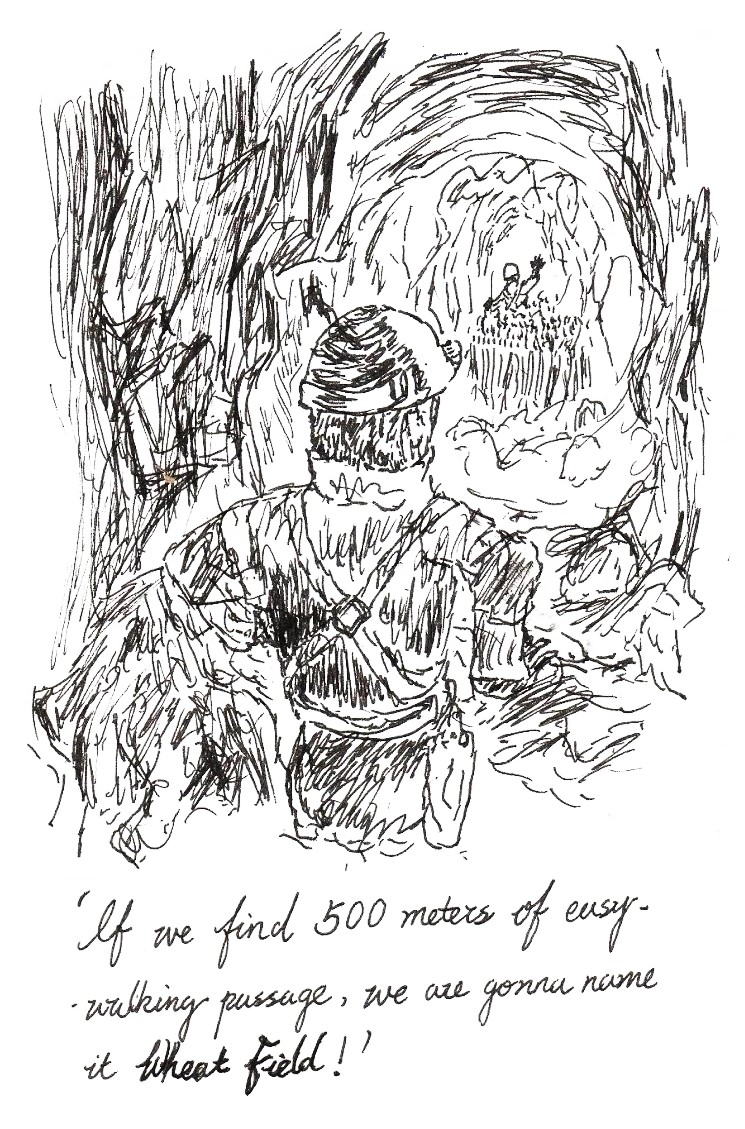
\includegraphics[width=0.9\linewidth]{images/overview/the_caver_2.jpg}
\caption{Drawn by Larry Jiyu Jiang}
\label{}
\end{pagefigure}
\newpage


\begin{tcolorbox} %makes a white opaque background for the text.
\vspace{60pt}
	\part{Introduction}
	\lettrine{S}{istem} \passage{Migovec}, tucked away at the western edge of the \passage{Triglavski Narodni Park} is the longest cave system in Slovenia.  It has held that title since 2012, when, defying expectations after a half a decade of effort, the connection between the `Old System' (\passage{M2}-\passage{M16}-\passage{M18}) and the newer \passage{Vrtnarija} (Gardeners' World) and \passage{Vilinska Jama} cave was forged after a routine pushing trip at -600m.

Thirty eight years after the first explorations underneath \passage{Tolminski Migovec}, or `Mig' as it is affectionately named, this connection made the national news. 

Since then, and rather more discreetly, Imperial College (ICCC) and Jamarska Sekcija PD Tolmin (JSPDT) cavers have repeatedly spent their part of their summers searching for more empty space under the Hollow Mountain. Bit by bit, other pieces of the puzzle were extended and connected to the main system.

In 2015, three Slovene cavers found a way between the \passage{Primadona}-\passage{Monatip}-\passage{Ubend571} cave system and one of the high level passages of \passage{Sistem Migovec}, bringing the sum total to 35.6km of interconnected passage. 

As of 2018, it stood at 39.2km, with, it is hoped, plenty more tales of exploration and adventure to come...

\mydelimiter

This book is divided in three parts. The introduction to the geography and geology of \passage{Tolminski Migovec}, the process of cave exploration and survey aims to give a cursory glance at the setting and logistics of the expeditions. This is followed by the main body of text: selected stories from expedition cavers, by no means a complete account of all the excursions under the mountain. These span the years 2013-2017, which saw systematic summer expeditions by ICCC and continuous JSPDT action. A third part provides a more detailed description of possible trips within the mountain, augmented with larger scale surveys: they are intended for expedition cavers craving to see more of this nearly 40km alpine system. 
\end{tcolorbox}
	\backgroundsetup{	scale=1,
					color=black,
					opacity=1,
					angle=0,
					contents={%
							  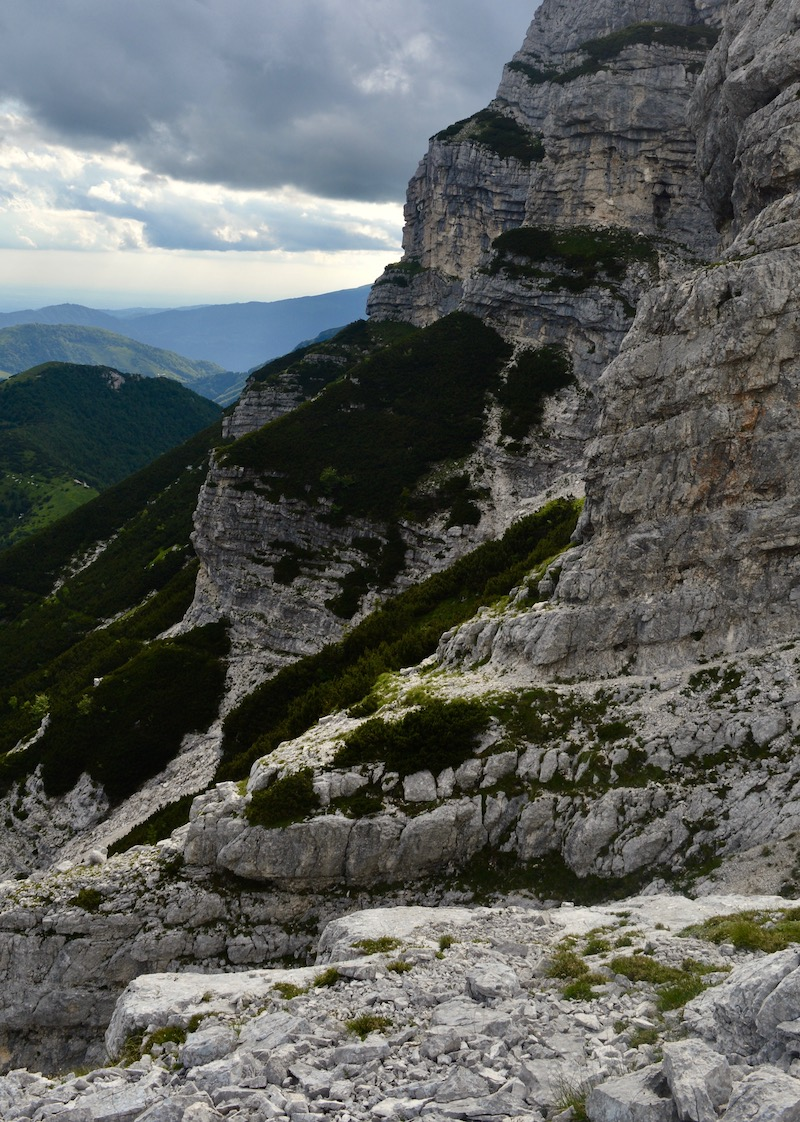
\includegraphics[height=\paperheight]{images/backgrounds/migface.jpg}
  					} % this puts the entire image as local background
	}
\BgThispage %calls the image to be displayed as background, flush with paper edge.

	\chapter{Overview}

\section{The pre-2013 story}
\textit{The following is a concise summary of exploration between 1974 and 2012.All intervening expeditions and findings are described in greater detail in The Hollow Mountain volumes I and II}

\subsection{1974-1994 --- The early days} The JSPDT members initiated exploration around \passage{Migovec} in 1974, with the logging of 17 caves entrances (\passage{M1} through to \passage{M17}). There were two notable findings: \passage{M2} - pushed from 1974 to 1978 - and \passage{M16} -pushed from 1982 and 1985, which at -350m and -547m were the then deepest caves of Yugoslavia, and contained a huge underground cavern named \passage{Galaktika}. After 1985, the JSPDT focused their man power on exploring the \passage{Mala Boca} resurgence. \passage{Migovec} was left virtually untouched for another decade. 


	\begin{marginfigure}
    \vspace{-250pt}
	\checkoddpage \ifoddpage \forcerectofloat \else \forceversofloat \fi
	\centering
	\frame{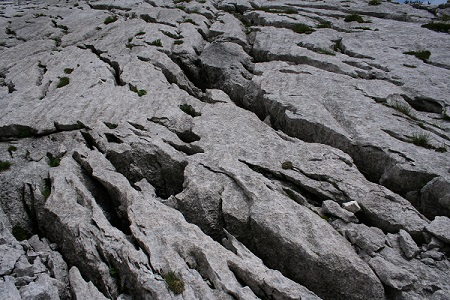
\includegraphics[width=\linewidth]{images/overview/jana_limestone.jpg}} 
  	\caption{A limestone pavement is where the story begins for the water, not so for cavers who prefer larger entrances to a cave system --- Jana \v{C}arga}
	\end{marginfigure}

\subsection{1994-2000 --- ICCC arrives in Slovenia} The first ICCC expedition to \passage{Migovec} took place in 1994; notable discoveries included \passage{M18} (cave of the \passage{Torn T-Shirt}), then 78m deep. The return visit in 1995 saw significant horizontal development (\passage{NCB passage}) and the set-up of a shallow underground camp (\passage{Club Mig}). This paved the way for several breakthroughs the following year and connection of \passage{M2}, \passage{M18} and \passage{M16}. 

\passage{Sistem Migovec} was born...

The following years saw a consistent probing of half a dozen different shaft series accessed by one single trunk route. Of these, only one (\passage{XXX}-\passage{Sajeta}) accessed deeper levels. Underground camping at \passage[camp]{Hotel Tolminka}.

\subsection{2000-2006 --- A new deep cave} In the year 2000 \passage{Vrtnarija} or \passage{Gardeners' World} entrance, which had been found several years earlier was dug out to reach a tight squeeze overlooking a loose pitch. Over the following days, pitch after pitch the cave continued gradually getting larger until \passage{Pico} pitch was discovered. This 10m diameter shaft plunged right into the heart of the mountain and carried both a strong draught and an anomalous amount of water 

Below \passage{Pico}, the 2000 and 2001 expeditions explored a clean-washed and well-watered shaft series spanning -200 to -500m, past some smaller pitches to reach \passage{Zimmer} (P50). At the bottom a horizontal passage beckoned: \passage{The Gallery of Anglo-Slovene Friendship}. Some 400m of easy passage, following the chilling draught then led to a black void, the tantalising limit of exploration for 2001.
    
We set up an underground camp camp in \passage{Friendship Gallery} in 2003 and set out to descend the new pitch \passage{Big Rock Candy Mountain}, and the passages below. Over the next two years, the abandoned, sandy fossil passages at depths between -700m and -800m led north into hitherto completely blank mountain, ending at a terminal looking sump, underneath \passage{Tolminski Kuk}.

During the 2004 derig --- a process where the ropes of the entrance series were brought up the pitches, and metalwork taken out the cave --- Tetley spotted a window off the side of \passage{Pico}, bolted a route and swung into what appeared to be an excellent new, shallow lead. The 2005 expedition focussed on this branch. Awkward pitches and tight passages were the bread and butter of \passage{Captain Kangaroo} explorers and was left as a major lead after an aborted camping trip toward the end of the expedition.

	\begin{marginfigure}
    \vspace{-250pt}
	\checkoddpage \ifoddpage \forcerectofloat \else \forceversofloat \fi
	\centering
	\frame{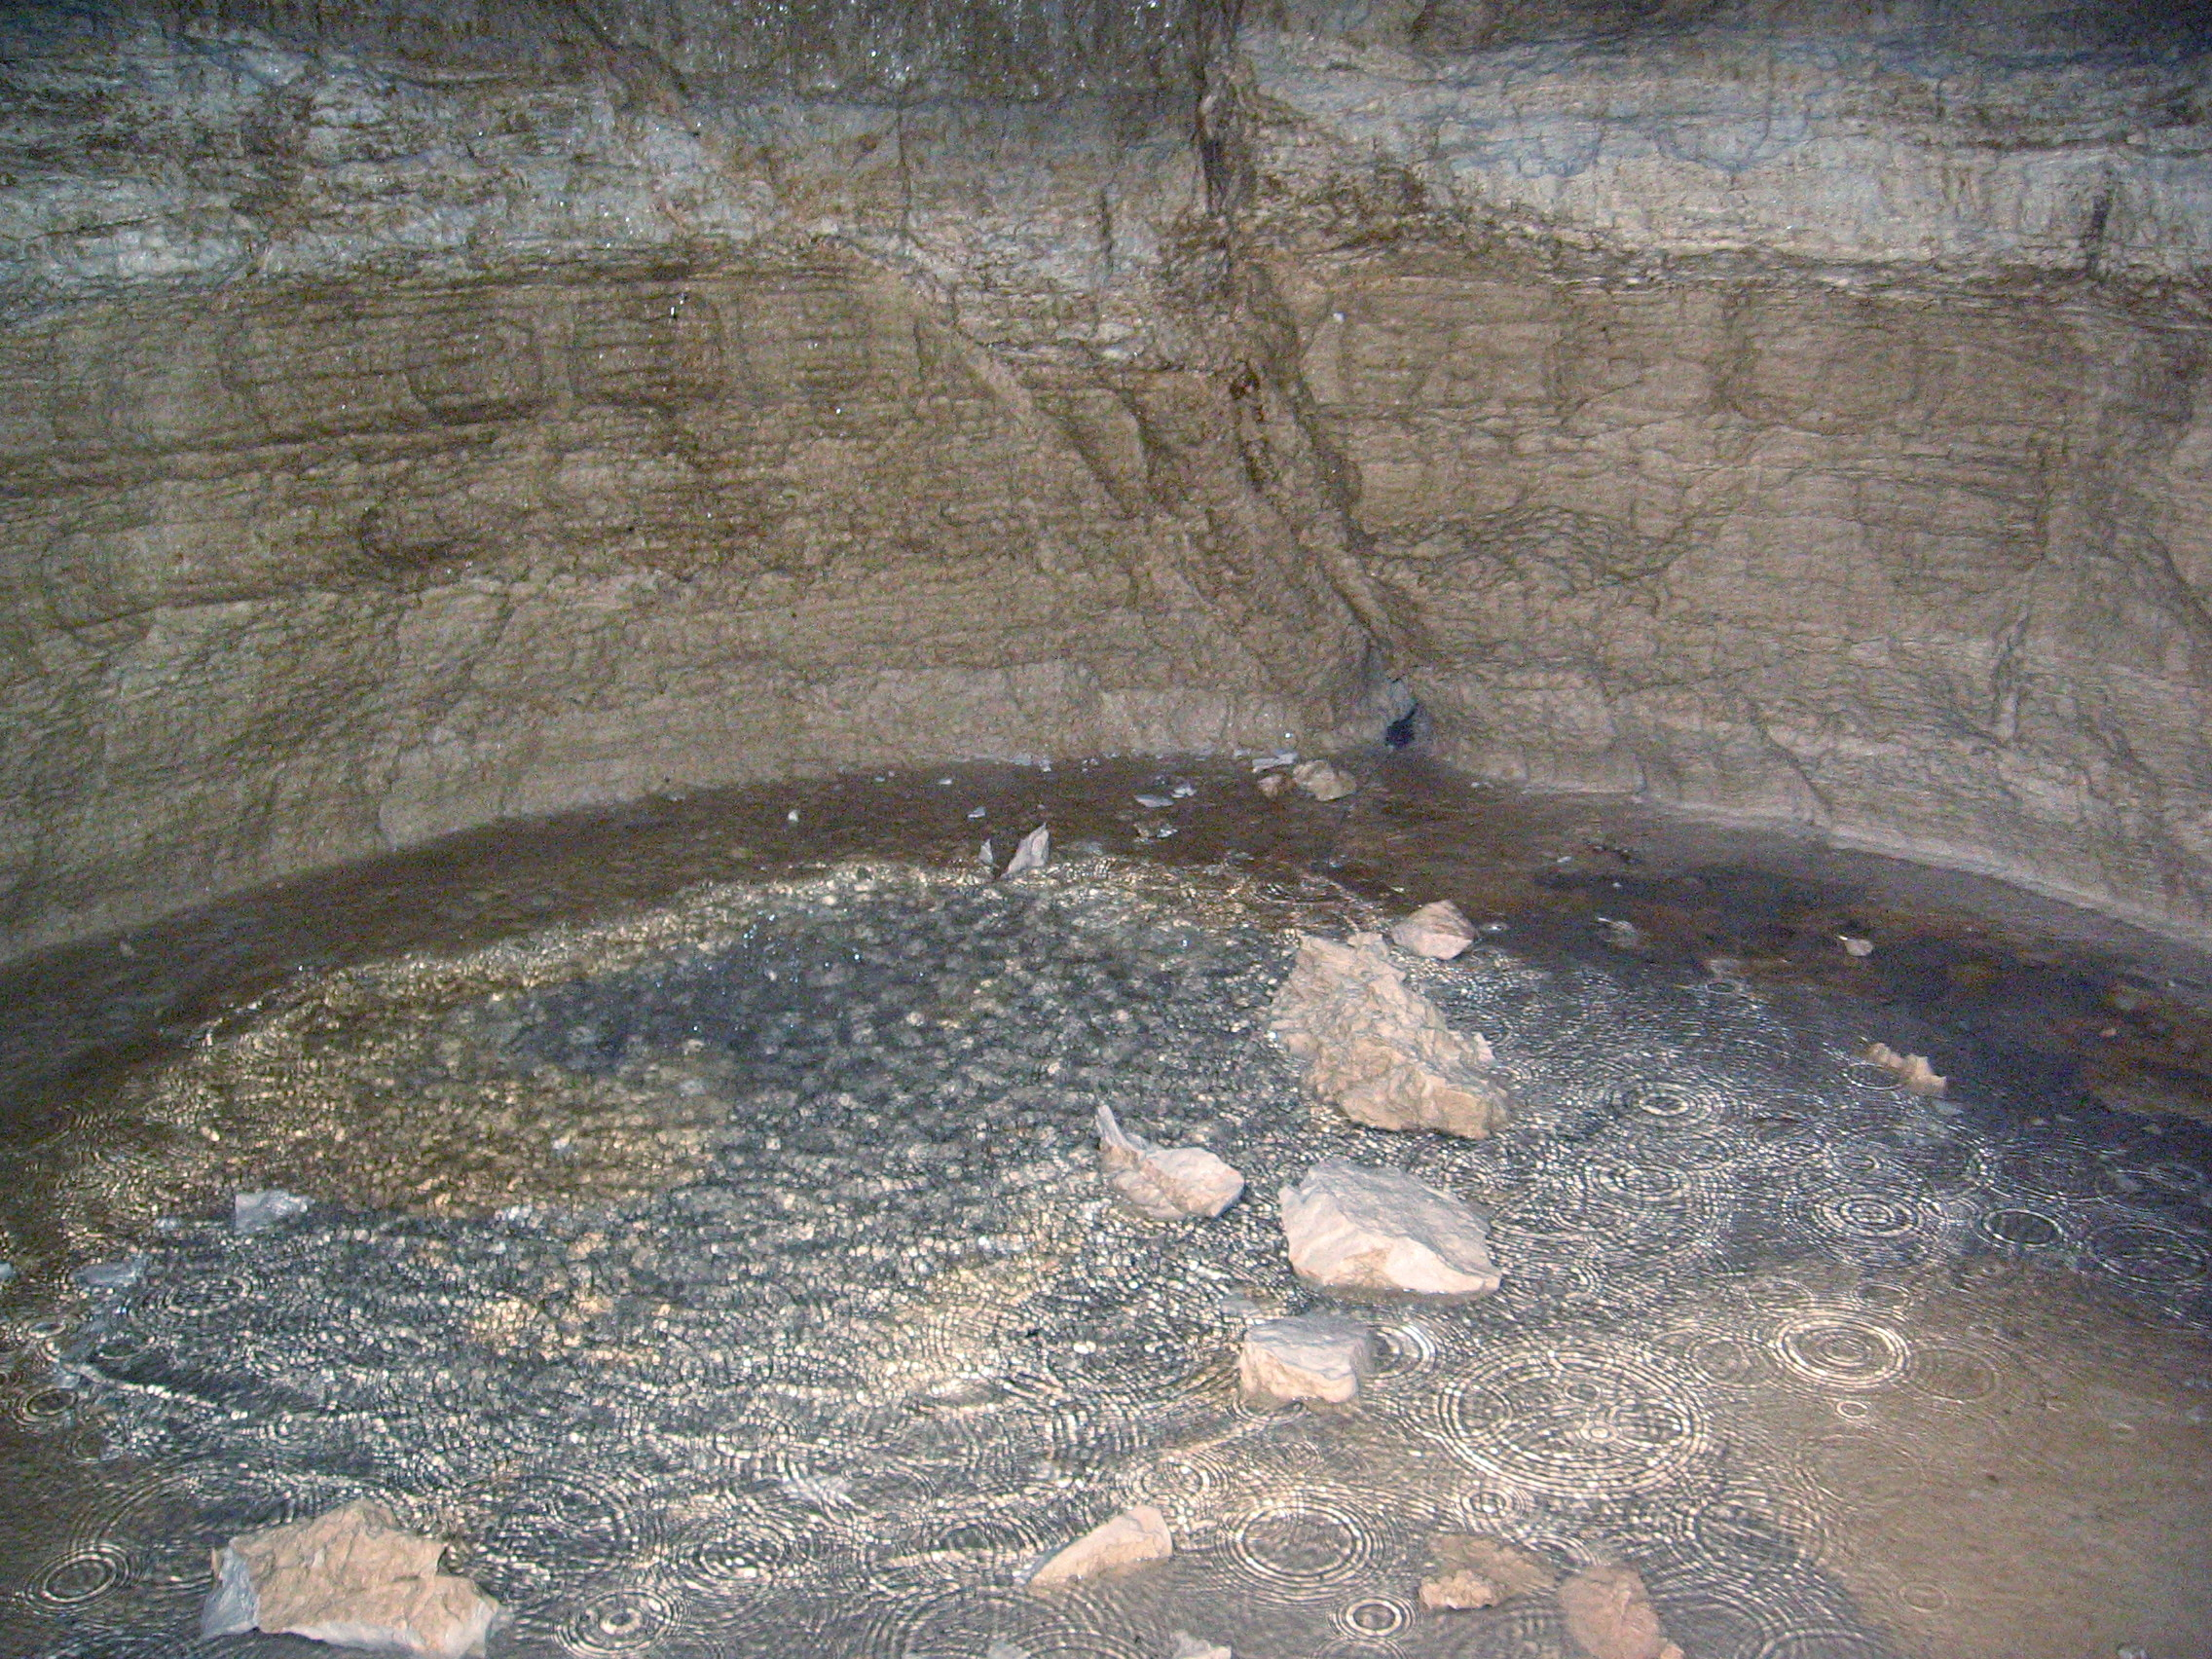
\includegraphics[width=\linewidth]{images/maps-of-mig/alchemy_drips_jana.jpg}} 
  	\caption{The bottom of \protect\passage{Alchemy} in \protect\passage{Vrtnarija} with is conspicuous flat floor and significant amount of water --- Jana \v{C}arga}
	\end{marginfigure}
    
    
\begin{marginfigure}
	\checkoddpage \ifoddpage \forcerectofloat \else \forceversofloat \fi
	\centering	\frame{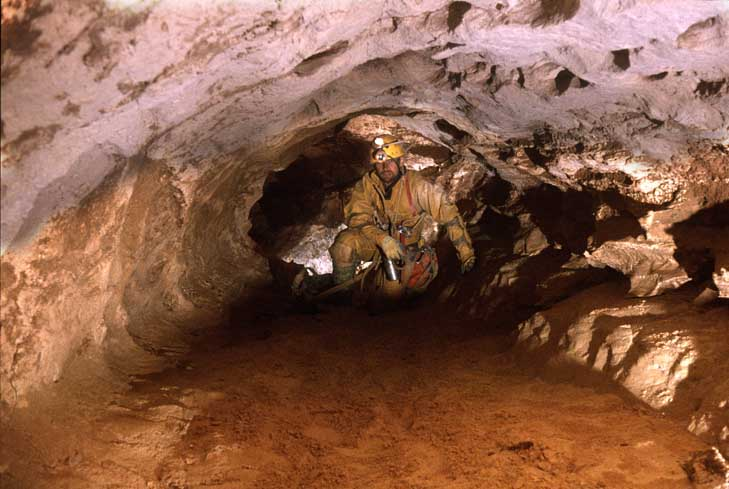
\includegraphics[width=\linewidth]{images/maps-of-mig/dw_highway32_oxbow.jpg}} 
  	\caption{The 2003-04 expedition findings included a plethora of interconnected passages below \protect\passage{Big Rock Candy Mountain} such as the sandy oxbow overlooking \protect\passage{Highway 32} streamway --- David Wilson}
	\end{marginfigure}

2006 was a year without ICCC summer expeditions, but Jarvist Frost and Jana \v{C}arga conducted an Autumn recce on the plateau, investigating the valleys to the west of the \passage{Plateau} as well as \passage{Area N}, a wilder plateau on the north side of \passage{Tolminksi Kuk}.

\subsection{2007-2009 --- Hard toil in Captain K branch} With plenty of new surface leads to push, the years 2007-2008 saw a concerted effort to find the next 'big cave' under the mountain. In parallel, the \passage{Captain Kangaroo} branch was extended further and found to head towards the bottom of \passage{M2} cave raising hopes for a connection between \passage{Vrtnarija}and \passage{Sysmig}, bringing the combined cave to just over 20km, thereby forging the second longest system in Slovenia as a reward for 15 years of nearly continuous exploration.

In 2009, \passage{Metal Camp} was set up in the newly found passages of \passage{Kill'em all}. Whilst no connection to M2 was made, the pitches increased in size again (\passage{Wet Hammer}, \passage{Mirage Canyon}, \passage{Happy Monday}), and dropped back to -550m, where a connection with \passage{Friendship Gallery} was forged. 

\subsection{2010-2012 --- A return to the deep Vrtnarija} 
\passage{M2} was revisited, its closest approach to Vrtnarija artificially enlarged over the course of several years. The two caves were well within survey error but no way through was found. 

Meanwhile, \passage{Friendship Gallery} was again used as a camp site location. On the back of the new improvements brought along with Metal Camp and with a 4 person hot-bedding system in place \passage{Camp X-Ray} became a palatial location: this played no small part in supporting true, deep alpine exploration.

%\lettrine{S}{istem} Migovec, tucked away at the western edge of the Trigavski Narodni Park is the longest cave system in Slovenia. It has been since 2012, when, defying the expectations after a half a decade of effort, the connection between the ‘Old System’ (M2-M16-M18) and the newer Vrtnarija (Gardener’s World) and Vilinska Jama cave was forged after a routine pushing trip at -600m. This - 38 years since the beginnings of exploration underneath Tolminski Migovec, ‘Mig’ as it is affectionately named - made the national news. 

%Since then, and rather more discreetly,  Imperial College cavers (ICCC) have repeatedly spent their summers discovering more voids under the hollow mountain, in tandem with the Jamarska Sekcija Planinskega Drustva Tolmin (JSPDT). Bit by bit, the other pieces of the puzzle were extended and connected to the main system. In October 2015, three Slovene cavers found a way between the last big independent cave system, Primadona-Monatip-Uben571 and one of the earliest high level passages of Sistem Migovec, bringing the total to 35.6km of connected passage. Since October 2017, it stands at 39.2km.

\section{2013 --- We’re not alone}

When the reports of a live creature sighting came back to the surface, they were first met with disbelief. Tetley, one of the long standing members of the expedition and Sam Page, a then second year student had spent several days underground, poking at the previous year’s ‘connection’ passages, hoping that in the rush for the finish line, side passages may have been missed. Since 2010, the expedition relied on camping in the \passage{Gallery of Anglo-Slovene Friendship}, a horizontal, abandoned phreatic 550m below the surface, a gallery from which it was possible to access the rapidly expanding pushing fronts under 3 hours. The entrance series to the cave was relatively hassle-free and direct, barring the ultimate pitch, whose spectacular free-hanging descent was ever so slightly wet, but this had its own advantages: it provided a ready source of water and untapped washing power; indeed any cutlery and cooking pots left for a couple of hours would inevitably come out spotless.

\begin{marginfigure}
	\checkoddpage \ifoddpage \forcerectofloat \else \forceversofloat \fi
	\centering	\frame{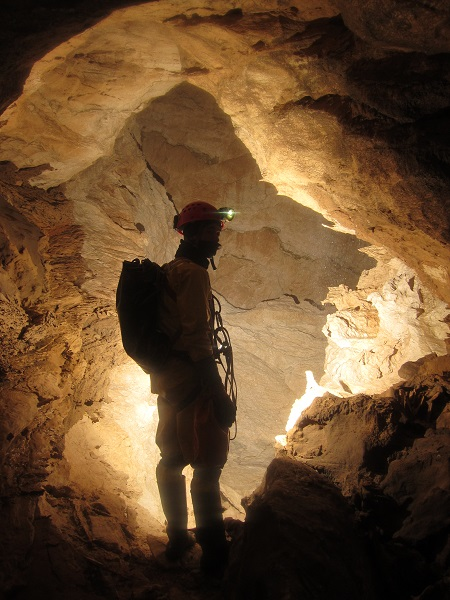
\includegraphics[width=\linewidth]{images/overview/rhys_red_cow.jpg}} 
  	\caption{A lot of the 2013-2015 exploration took place in the deep \protect\passage{Vrtnarija} levels --- Jarvist Frost}
	\end{marginfigure}

It was from this palatial camp that the exploratory duo went for a visit to the southern branch of the system, a series of muddy, but essential bone dry, strongly draughting and horizontal galleries. Recent extensions were headed due south, along an old phreatic tunnel, modified by breakdown in places, and, extraordinarily for this particular alpine system, decorated with stalactites. The encounter happened at one of the rare spots where water trickles in from the roof, right at the foot of an extremely muddy pitch. They caught a glimpse of a live dormouse, furry tail and all, right at the heart of the mountain and lived to tell the tale. Where had it come from? 

While this question did not fuel a mad break for the surface, steady exploration of the southern branches by Rhys Tyers, Dave Kirkpatrick, Clare Tan and myself over the following years yielded more and more evidence that these mammals do occasionally wander into and litter our cave system.

\section{2014-2015 --- The cave goes South}

In 2014, we went further into the \passage{Atlantis} branch, finding a sizeable stream at the far end of the large, sediment filled \passage{Helm’s Deep} chamber. The interest went soon over to a north-south oriented rift, draughting very strongly outwards and heading towards the southern face of \passage{Tolminski Migovec}. This puzzled us for a while: a vertical maze of climbs and drops where metres of passage were hard won. There, we first found the mouldy remains of dormouse at the foot of a small climb. For want of rope and time, we left this for the next expedition to resolve.

2015 saw us eager to find a way out of the cave: the first trip had found more rift, bringing the surface to fewer than 500m horizontally. On the surface, Jack Hare plotted the known end of the cave against the topographical map, and with rough coordinates in the GPS set out to discover the lower entrance. This was successful: by climbing up a N-S oriented canyon, he and Rhys stumbled upon a possible opening which had a good draught, whistling through a mud and boulder blockage. 

I arrived late on the expedition, but soon got underground with Rhys, motivated to push the southern end as well. We quickly broke through a choke, descended a 25m pitch where I pointed out the exposed fault planes which had obviously guided its current morphology, and at the bottom rejoined the main, abandoned phreatic level, stretching all the way to \passage{Atlantis} for more than a kilometre. This led us south, and excited as we were to be treading the easy walking passage of the \passage{Meridian Way}, we couldn’t help but notice scratch marks, hair, bones and excrement littering the gallery floor. The next team pushed this even further, getting to within 250m from the surface. Next up was a constriction that would need time and effort to pass.

But this was it for the lower entrance story: turning back from that part of the cave, we had 4-5hrs caving to reach the camp, and that again to get back out on the surface. At the end of the summer 2015, we collectively decided to shift our objectives and luckily, a completely new training ground had opened up to us.

\section{2000-2015 --- The twelve battles of Monatip}
Back in the early 2000’s, while ICCC were busy pushing \passage{Vrtnarija}, entering the mountain from the eastern side, cavers from the JSPDT investigated a large entrance situated half-way down the western cliff, named \passage{Primadona}. Early day trip explorations extended the cave to over 600m in depth, and it wasn’t until 2007 that another entrance  on the cliffside, roughly 100m north was spotted: this became \passage{Monatip} cave. The system proved a training ground for the younger members of the JSPDT from 2008 onwards, after these two western caves were connected. Exploration picked up in earnest after the well publicised 2012 connection as the added 5km of \passage{Primadona}-\passage{Monatip}-\passage{Ubend571} would put \passage{Sistem Migovec} out of reach of its more famous contender, \passage{Postojnska Jama}, but many cavers doubted there could be a connection, due to a large surface fault, coinciding with hitherto unexplored, blank mountain. The way did exist however.

One of the key members of the later exploration of \passage{Monatip} was Dejan Ristic, who, over the course of twelve assaults, therefore mirroring the more sinister WWI Soča battles, forged the connection between \passage{Monatip}, and \passage{Sistem Migovec}. Together with Andrej Fratnik, long-standing \passage{Migovec} explorer and Iztok Mozir, they traversed, and squeezed and dug, and eventually emerged in \passage{NCB} passage. This ground, first tread in 1995 by ICCC cavers had proved time and again critical in the connection stories of the \passage{Migovec }caves, it’s discovery playing no small part in the early survival of the IC expeditions. The successful trio fittingly exited via \passage{M2}, the oldest explored entrance which is kept permanently rigged.

	\begin{marginfigure}
	\checkoddpage \ifoddpage \forcerectofloat \else \forceversofloat \fi
	\centering
	\frame{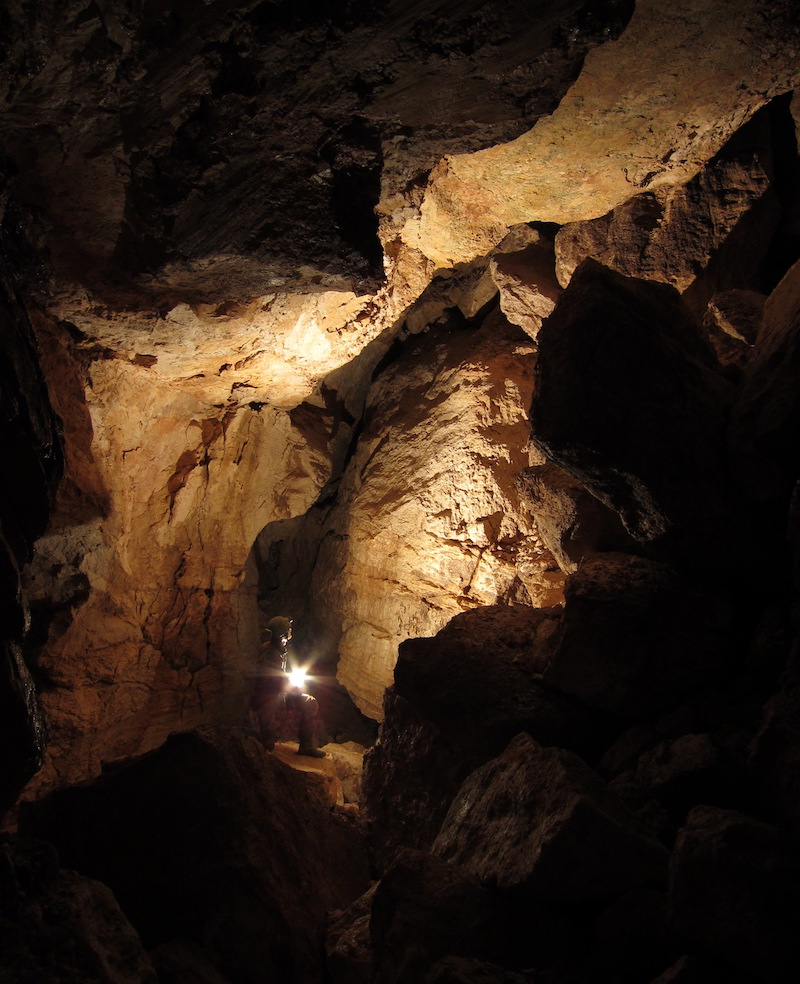
\includegraphics[width=\linewidth]{images/2017/tanguy-hammerhead-2017/hammerhead-chamber.jpg}} 
  	\caption{Discovery of \protect\passage{Hammerhead} chamber one of the later findings of 2017 --- Jarvist Frost}
	\end{marginfigure}

\section{2016 --- The road less traveled}
This is how things stood in the closing months of 2015. Plans to move to the deeper, and possibly still fertile ground of \passage{Primadona} were formed. Some of the newer expedition members, myself included wanted to start bolting deeper pitches, and the rerigging project we formulated provided just that. We would be able to take novices on easier bounce trip, allured by the promise of shallow leads left unpushed in a bid for greater depth.

The cave, while far from perfect provided many surprises. For almost all of the IC cavers, this was \textsl{terra incognita}  from the onset. Why, it took us four days, and an aborted attempt down the wrong valley to locate and reach the entrance. By that time, I’d put in more bolts with a drill than for two previous expeditions, but then, we got some help from the JSPDT. Zdenko, aside from bringing the appreciated \v{Z}ganje and local deer sausage, showed us the way on, giving names to places, which we shamefully Anglicised. \passage{Sejna Soba}, the meeting room, became ‘\passage{Sane and Sober}’ something Migovec cavers as a whole cannot be accused of being. He showed and pointed at openings ‘I’ve never been, we think it goes towards X… always go left you will find blank mountain...’ Clearly, there was potential.


\begin{marginfigure}

	\checkoddpage \ifoddpage \forcerectofloat \else \forceversofloat \fi
	\centering
	\frame{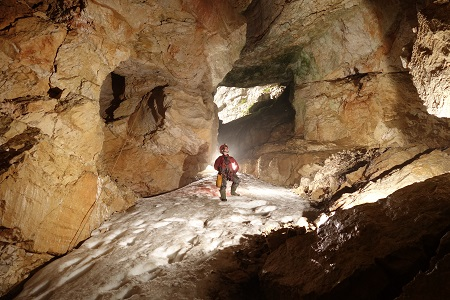
\includegraphics[width=\linewidth]{images/overview/rhys_diss_prima.jpg}} 
  	\caption{Woo! \protect\passage{Primadona} --- Rhys Tyers}
	\end{marginfigure}

We pooled our newly gained knowledge of the cave and to our surprise we started treading new ground: pitches which had been rigged but not descended, obscure climbs which led to vast caverns, a parallel shaft series which we connected back to the old way down deep. And somehow, the old objective of going down deep was forgotten: we were side tracked at every level by a complex series of connected, horizontal passages. Yet, the almost mythical left turn into blank mountain eluded us.

\section{2017 --- Divine intervention}
The 2017 team approached the cave differently. For the returning cavers, the novelty had worn off, we’d mulled over our best leads during eleven months, and we were keen to make our knowledge count. So we almost tacitly concentrated our efforts to three areas of\passage{ Primadona}: the \passage{Galerija}, \passage{TTT} and \passage{Fenestrator} branches.

The \passage{TTT} branch, which I’d become familiar with in 2016 was the original way to the deepest point of \passage{Primadona}. A side passage which I’d spotted led to a series of chambers and pitches, ending in a draughting, high aven where the boulder collapse was pervasive. We ran out of steam there: the trips were long and strenuous, the cave never particularly friendly.

Over to the west, Jack Hare bolted a metal-rich traverse over a 40m drop to gain the continuing horizontal passage at the far end of \passage{Galerija}. This was very successful and promising: a memorable push led to increasingly large pitches (P5, P10, P22), ending at yet another drop. Eventually, this provided a stunning abseil through the roof of the \passage{Hall of the Mountain King} (P42), a cavern found the previous year: the exploration met a satisfying end.

It was further up the cave, very close to a small rest-stop we’d set up - and nicknamed\passage{Mary’s Caf\'{e}}- that the most significant discoveries of the year took place. Little by little, an obscure SE trending rift led away from the main tangle of passages. Ever changing in nature, now a muddy phreatic (\passage{Plumbers' Paradise}), now a vadose stream (\passage{Hallelujah}), now a clean-washed pitch series (\passage{Sweet Baby Jesus}), this branch extended far into the blank mountain we’d been advised to explore.  

\begin{marginfigure}
\vspace{-200pt}
	\checkoddpage \ifoddpage \forcerectofloat \else \forceversofloat \fi
	\centering
	\frame{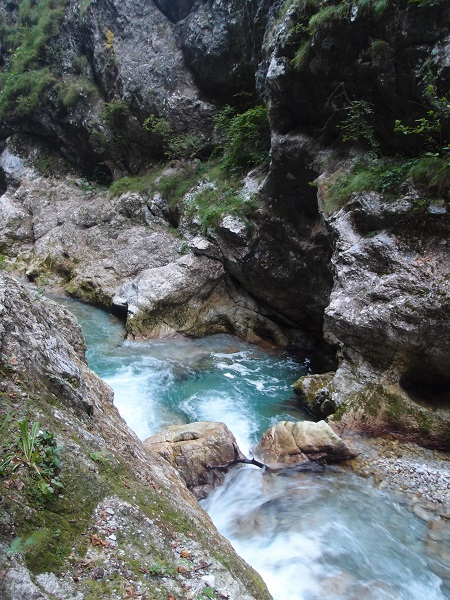
\includegraphics[width=\linewidth]{images/overview/tolminka_cecilia.jpg}} 
  	\caption{Precipitation in the high limestone ranges finds its way underground and resurges as two stunningly blue streams: the \protect\passage[river]{Tolminka} and \protect\passage[river]{Zadla\v{z}cica} rivers, photographed near their confluence --- Cecilia Kan}
	\end{marginfigure}

\section{The outlook}
So what next? There's plenty of interest for the upcoming the 2018 expedition, where we hope to be camping in \passage{Primadona} and finally push the deeper levels. One thing is for certain, the successful annual expeditions have helped cement a true club spirit and prepare the newer cavers for the leadership roles they naturally assumed coming back to the UK. 

\name{Tanguy Racine}

	\chapter{The cave areas of Migovec}
\begin{marginfigure}
\checkoddpage \ifoddpage \forcerectofloat \else \forceversofloat \fi
\centering
\vspace{50pt}
 \frame{\includegraphics[width=\linewidth]{"images/maps-of-mig/migovec-alongside-andy".jpg}} 
 \caption{The \protect\passage{Migovec Plateau} and a panorama to the south over the \protect\passage{Dinarides} \pic{Andy Jurd}}
 \label{dinarides}
\end{marginfigure}

\section{The Hollow Mountain}
The silhouette of \passage{Tolminski Migovec} is like an old friend to the inhabitants of nearby villages and alps. The sheer cliffs endure the passing of the seasons, while all around, the alpine meadows and pine forests grow boldly green or retreat and sometimes hide under a thick blanket of winter's snows. Its rough crevices, imposing limestone buttresses and bare scree cones impart an austere look on the unmistakable southern precipice, the face \passage{Tolminski Migovec} shows to the casual walkers.

This mountain of \passage{Tolmin} is reared up against a limestone ridge higher still, as if a promise of a larger barren wilderness, towering at 1862m elevation above the \passage{Tolminka} valley. \passage{Mig} lies at the western edge of the \passage{Triglavski Narodni Park} (\passage{Triglav National Park}). 


 \begin{pagefigure}
 \checkoddpage \ifoddpage \forcerectofloat \else \forceversofloat \fi
\centering
  \frame{\includegraphics[width=\textwidth]{"images/maps-of-mig/jana_carga_migoec_in_winter".jpg}}
  \label{winter panorama migovec}
  \caption{\protect\passage[cave]{Tolminski Migovec} in Winter, as seen from a popular paraglider spot looking north \pic{Jana Čarga}}
 \end{pagefigure}

The ascension to the summit, a three to four hour walk from the city of Tolmin rewards the curious walker with gorgeous views of the limestone landscapes of the \passage{Julian Alps}. To the south-west, spanning the bay of \passage{Trieste}, the unbroken flatness of the Italian plain scintillates with a myriad of urban lights after dark. South is a world of gentle, rolling hills, merging into the sky in a blue haze; a humped mass in the distance marks the border with Croatia. 

The east is barred from view by a line of jagged high peaks, clawing at the sky with bare grey knuckles. On the other side, another country almost: water drains to form the \passage\protect{Sava} river, collecting in the glacial lake \passage[lake]{Bohinj}, then flows past \passage{Ljubljana}, the capital, towards the \passage{Black Sea}. As if calling to \passage{Migovec} from the other side of the \passage{Tolminka} valley to the north-west, the high ramparts of \passage{Krn} swallow the setting sun between their irregular crenels.

The mountain is made up of a mass of titled limestones, bounded to the west by two flights of white, jagged cliffs at 700-900m and 1600-1800m respectively, and to the east by an elongate glacial cirque. From the foothills of \passage{Migovec}, water resurges through several boulders filled canyons, emerging from the fissures that guided its underground course. It takes the name \passage{Zadla\v{z}\v{c}ica} where it springs to light.  

The surface of the undulating, 1x2km \passage{Plateau}, riddled in places with potholes as much as 30m deep. These obvious depressions, unmistakable signs of karstic landscapes - this means that dissolution of soluble rocks is the major driver of erosion  - are so many potential thresholds to the hidden worlds inside the mountain.

\margininbox{Did you know?}{A glacial cirque is a theatre shaped valley formed by glacial erosion, with steep uphill sides, and a shallower downhill slope. By contrast, large `ampitheatre shakeholes' on the mountain are a result of karstic processes, where the uphill slopes are generally shallower and assume the angle of repose of stacked scree}{\logbook}. 

\section{Local geography}
In the following article, different cave areas around \passage{Migovec} are introduced. Their commonly used names arose from history of exploration and geographical significance. This attempt to give a useful, unified account of geographical names is by no means exhaustive; for cave specific research, we refer the reader to the index of colloquial names, located at the end of the book.In the body of text, the named passages are \smallcaps{highlighted thus}.

\subsection{The M-series} 
The M-series as the caves found mostly on the Migovec Plateau and were first explored during the 1974-1994 period. This area encompasses the undulating surface of the Migovec Plateau, as far north as the start of the rise towards \protect\passage{Tolminski Kuk}, and as far south as the main \protect\passage{Limestone Pavement}, a significant depression between \protect\passage{Tolminski Migovec} and the camping spots (see map \ref{map overlay}).


\paragraph{Overview} Exploration of \passage{Sistem Migovec} by the \textit{Jamarska Sekcija Planinskega Društva Tolmin - JSPDT}, \fref{map:map overlay} hereafter referred to as the JSPDT, began in earnest in 1974, under the impulse from longstanding members Zoran Lesjak, Brane Bratuž, Stanko Breška and Fischione Alfonz \citep{hm1}. They started exploring, digging and bolting down the main shakeholes of Area M (for Migovec), naming and numbering their most promising leads at the time (\passage{M1} to \passage{M17}). More M number caves were added during the 1994 \textit{Imperial College Caving Club} (ICCC) expedition (M18-M24). Below is a short discussion on the most significant of the M-series caves (see \citet{hm1} for complete details). 

\begin{marginfigure}
\checkoddpage \ifoddpage \forcerectofloat \else \forceversofloat \fi
\centering
 \frame{\includegraphics[width=\linewidth]{"images/maps-of-mig/m2_entrance".jpg}} 
 \caption{The snow plug entrance of M2 is the highest of the eight ways into \protect\passage{Sistem Migovec} \pic{Tanguy Racine}}
 \label{surfaceM2}
\end{marginfigure}

\begin{marginfigure}
\checkoddpage \ifoddpage \forcerectofloat \else \forceversofloat \fi
\centering
 \frame{\includegraphics[width=\linewidth]{"images/maps-of-mig/prima-ent".jpg}} 
 \caption{The large (by \protect\passage{Migovec} standards) entrance of \protect\passage{Primadona}, found off the west cliff of the \protect\passage{Plateau} whose exploration is dealt with in the 2016 and 2017 exploration entries \pic{Rhys Tyers}}
 \label{surfaceM2}
\end{marginfigure}

\paragraph{M2} Early on, \passage{M2} or \passage{Kavka Jama} (Jackdaw Cave) was explored to a depth of -350m, and comprised a 120m unbroken and impressive shaft named \passage[pitch]{Silos}. The twin entrances to the cave lay to the east of the Plateau: a sizeable shaft plugged with snow letting light into the main entrance chamber connected to a smaller, free-climbable rift entrance. The termination of M2 at the time was an artificially enlarged squeeze at the end of a draughting, narrow rift with clear depth potential.

\paragraph{M16} In 1982, and after significant digging effort, \passage{M16} was broken into. A 100m to the SW of \passage{M2}, and a stone's throw from the massive, but unfortunately choked M1 gaping entrance, a small, choss filled tube led to the start of a long pitch series, extending down to -547m. The jewel of the cave which, unusually at time ranked as one of the deepest in Slovenia, was the final chamber \passage{Galaktika}, the largest underground volume yet under \passage{Tolminski Migovec}. 



\paragraph{M18} This area of shakeholes yielded many other caves in the mid 1990s when the Imperial College Caving Club started to systematically explore the mountain. \passage{M18} or \passage[|see{Torn T-Shirt}]{Jama Strgane Srajce} cave, with its entrance less than 10m away from \passage{M2} developed into a sharp canyon until the key \passage{NCB} breakthrough, which enabled two major connections to be forged between \passage{M18}, \passage{M2} and \passage{M16}. Together, these formed \passage{Sistem Migovec} otherwise known as the \passage{Old System}. Through the \passage{M16} entrance, exploration focussed on the deep end at first, with separate sumps encountered near $-969m$ depth and shifted towards the shallower pitch series, with new passage adding up to over $11km$ of cave, most of it vertical.

As shown on the Area M \vref{map:map overlay}), many other blowing holes, potential cave entrance and caverns of (as yet) lesser significance were pushed, named and surveyed over the years. Early ICCC cavers continued in the tradition of the M-series, going up to \passage{M24}. \fref[margin]{sec:early history}

\subsection{Vrtnarija} Dropping further down the eastern glacial cirque, to the NE of the aforementioned entrances lies \passage{Vrtnarija} also known as  \passage[|see{Vrtnarija}]{Gardeners' World} cave. Though spotted in 1996, the key breakthrough occurred in the year 2000, when a deep pitch series quickly dropped to -350m and was left ongoing. The following year ended on the discovery a long horizontal gallery at -550m, which provided the ideal campsite for the next decade of joint cave exploration between ICCC and the JSPDT. \fref[margin]{sec:early vrtnarija}. 

\subsection{Sistem Primadona} At the opposite edge of the Plateau, and accessed via either a 120m clif f abseil or a steep scree climb, the large entrance of \passage{Primadona} was the gateway to another significant system. The cave filled a blank area of mountain far to the west of Sistem Migovec. \fref[margin]{sec:early primadona}

\subsection{The S- series} This collection of caves lies down in   the \passage{Gardeners' World} valley. In 2013 the numbers 5-7 were added to the list, but it is S1 which has received the most attention so far. Sporadic exploration over the years (up until 2017) met an ascending boulder choke obstacle issuing a very cold draught, which due to the pushing front's proximity with M16, was attributed to the same air as flows through the end Hotline gallery to the North West. 





%\begin{marginfigure}
%\checkoddpage \ifoddpage \forcerectofloat \else \forceversofloat \fi
%\centering
 %\frame{\includegraphics[width=\linewidth]{"images/maps-of-mig/m16 entrance".jpg}} 
 %\caption{Due to its ease of access M16 is the chosen entrance for visits to the \emph{Old System} ---Rhys Tyers}
% \label{surfaceM16}
%\end{marginfigure}


%\begin{marginfigure}
%\checkoddpage \ifoddpage \forcerectofloat \else \forceversofloat \fi
%\centering
% \frame{\includegraphics[width=\linewidth]{"images/maps-of-mig/m17-m19".jpg}} 
% \caption{Surface potholes like M17 and M19 can reach 30m depth ---Tanguy Racine}
% \label{surfaceM17}
%\end{marginfigure}


\begin{pagemap}
 \checkoddpage \ifoddpage \forcerectofloat \else \forceversofloat \fi
\centering
  \includegraphics[width=\textwidth]{"images/maps-of-mig/system_overlay".png}
  \caption{Cave passage and topography of Tolminski Migovec, Slovenian National Grid ESPG 3794}
   \label{map:map overlay}
 \end{pagemap}


 

	


\chapter{Geology of Migovec}

\section{The Julian Alps}
\label{sec:The Julian Alps}

\subsection{Geography} 
\label{par:Geography} 
\passage{Tolminski Migovec} belong to the \passage{Julian Alps}, in the easternmost sector of the \passage{Southern Alps} \citep{bavec2004late}. 
They \passage{Julian Alps} are bounded by the Pannonian and  Fruili-Veneto bassins to the east and west respectively, while to the north, they are separated from the \passage{Eastern Alps} by the Periadriatic lineament\fref{map:geol large scale}. Southward from the South Alpine front, they become the \passage{Dinarides} \citep{placer1998contribution,burrato2008sources}.
This carbonate dominated massif is characterised by high relief with valley floors located 100-400m asl and peaks in excess of 2000m asl  \citep{vsmuc2009tectonic}. Relief production is attributed to both tectonic processes and glaciation, and \citet{vsmuc2009tectonic} argue for the primacy of the litho-sructural setting for the observed meso (1-10m) and macro- (100-1000m) scale relief.


\subsection{Structural style}
\label{par:Structural style}
Overall, the tectono-stratigraphic setting \sidenote{The interplay between relief generation, erosion and sedimentary deposition during \emph{orogenesis} or moutain building events} of the \passage{Julian Alps} is a result of continued northward motion (about 2mm.a$^{-1}$ \citep{burrato2008sources} and since the Miocene,  counter-clockwise rotation of the Adriatic microplate \citep{marton2003palaeomagnetic}. 
The convergence of the Adria microplate with the Eurasian plate is quantitatively described by GPS velocity fields \citep{grenerczy2005tectonic}. 
Such convergence was led to the formation of Alpine and Dinaric mountain chains, and still generates earthquakes today ($M_w$ > 5) in the brittle deformation zone.

Slovenia, and in particular the area north east of Tolmin are located in the north-eastern corner of the Adria-Europe collisional belt. 
This area, at the critical juncture between the Alpine and Dinaric chains overlook rim of high topography around the relatively rigid, undeformed Adria microplate, which is only exposed in the Istria peninsula \citep{vsmuc2009tectonic}. 
It is buried under a thick cover of foredeep \sidenote{Foredeep basins form in the immediate vicinity of collisional belt as thickened crust deforms the somewhat elastic plate underneath, creating a trough where the material sourced from the nearby mountains is preferentially deposited}sediments in the Friuli-Venetian plain. 

It is useful to define a hierarchy for the subdivision of tectonic units within the Tolmin area. 
At first order, the \passage{Southern Alps} lie between by the Periadriatic lineament and South Alpine front \citep{placer1998contribution}. 
Second order units, e.g. the Zlatna, Julian (locally Krn) and Tolmin nappes are slices bounded by south verging thrust faults. 
This reverse thrusting resulted in an inversion of stratigraphical order, and place massive upper Triassic limestones at the top of the sequence, while the Jurassic/Cretaceous marls and limestones of the Tolmin nappe crop out at much lower elevation.

\begin{map}[b!]
\checkoddpage \ifoddpage \forcerectofloat \else \forceversofloat \fi
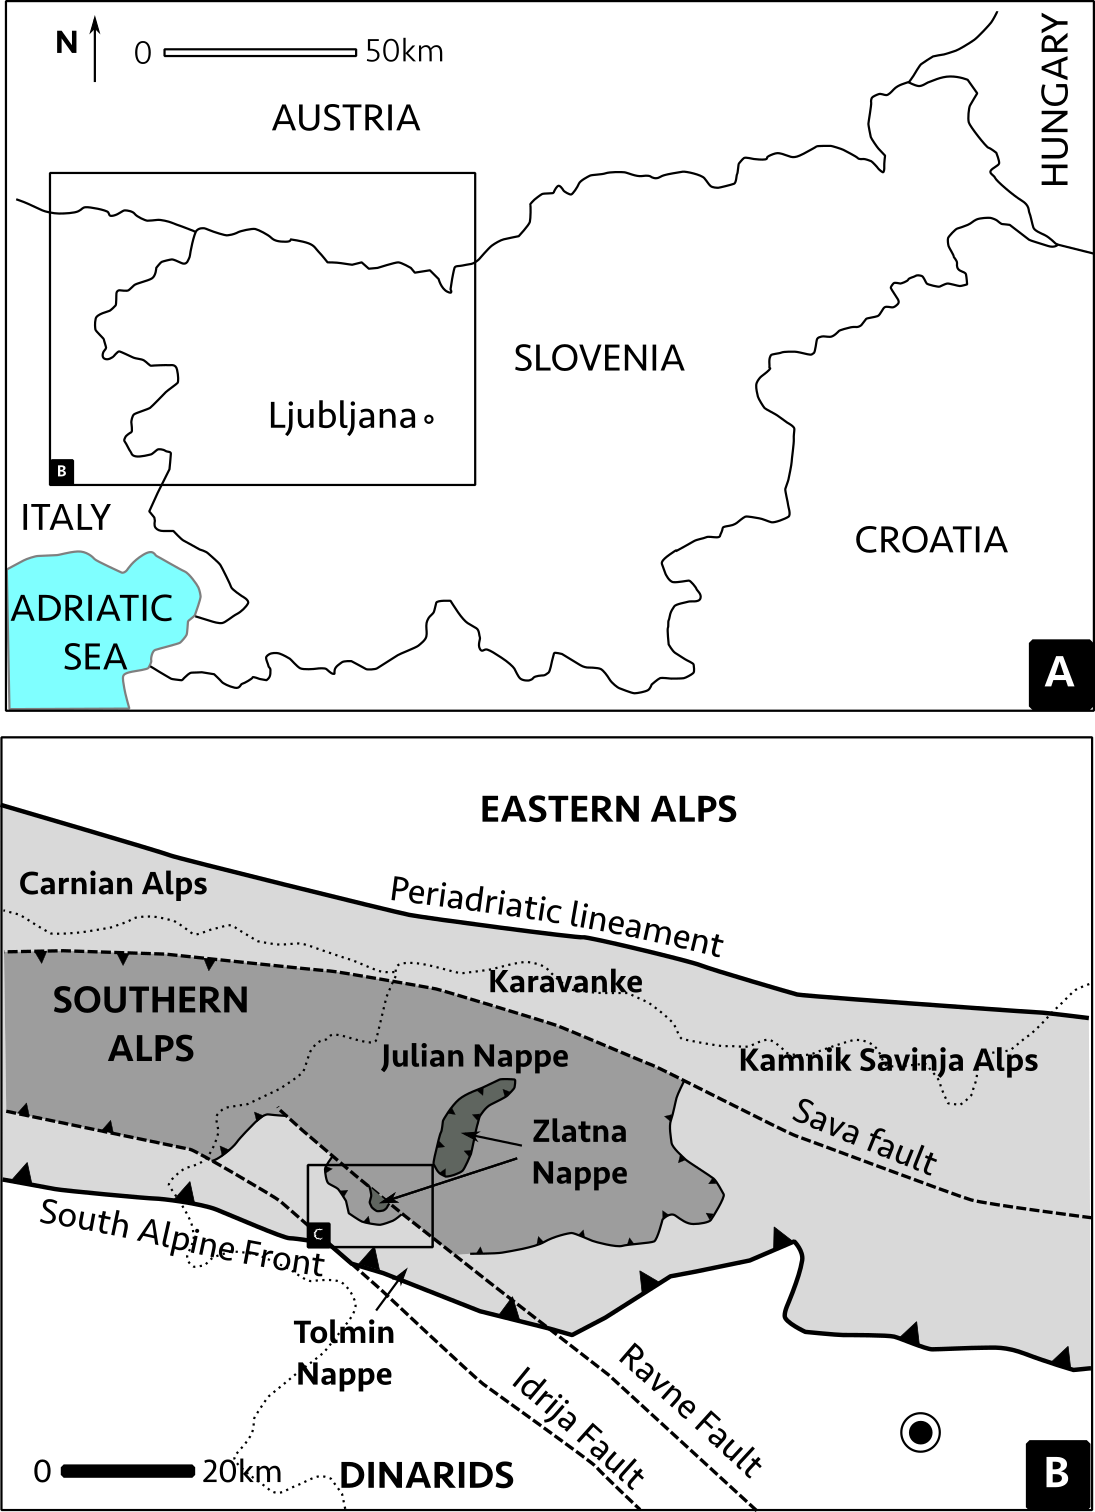
\includegraphics[width = \textwidth]{images/maps-of-mig/geology_large.png}
\caption[Structural setting of NW Slovenia]{\emph{(a)} Overview map of Slovenia \emph{(b)} The structural setting of northwestern Slovenia shows the \protect\passage{Tolmin} area straddling the active \protect\passage[fault]{Idrija} and \protect\passage[fault]{Ravne} faults. The \protect\passage{Migovec System} is developed within the Slatna overthrust and the underlying Dachtsein limestone, as shown in the geological map from \citet{buser1986tolmavc}. Figure modified from \citet{vsmuc2009tectonic}}
\label{map:geol large scale}
\end{map}


 
\subsection{Alpine deformation}
\label{par:alpine deformation}
That the \passage{Julian Nappe}, which comprises the cave forming Dachstein Limestones of the \passage{Krn}-\passage{Migovec} area was transported towards the south during the Alpine orogen is commonplace in the litterature \citep{doglioni1987eoalpine,placer1998contribution}. 
The weak and easily deformed Carboniferous clastics basement of the \passage{Julian Alps} provided a detachment horizon along which the nappe was transported from the north southwards. The question of the timing of transport of this nappe is somewhat more difficult. \citet{buser1986tolmavc} attributes a Neogene (~23Ma to 3Ma BP) age to this tectonic structure, while \citet{placer1998contribution} argues it could be slightly older, starting in mid to Late Oligocene (28Ma BP).

\subsection{Present day stress regime}
\label{par:present day stress regime}
The activity on this heavily faulted boundary between Adria and Eurasia is highlighted by recent destructive earthquakes: $M_w$=6.4 on the Italian side in 1976 \citep{pondrelli2001seismotectonic}, and $M_w$=5.7 and $M_w$=5.2 on the Slovenian side in 1998 \citep{bajc20011998} and 2004 \citep{aoudia2005july} respectively. 
To highlight the vulnerability of this region, it is also worth keeping in mind that the largest earthquake ever at this junction between the \passage{Southern Alps} and the \passage{Dinarides} was the 1511 western Slovenia earthquake ($M_w$= 6.8). It is believed to have resulted in at least 12,000 deaths \citep{fitzko2005constraints}.
Fault plane solutions for the many $M_w$=4-6 regional quakes demonstrate that the mode of deformation on the Italian side is chiefly by thrusting \citep{poli2002new}, while deformation is accommodated by dextral slip on the Slovenian side \citep{poljak2000seismotectonic}. 
The main strike-slip faults in NW Slovenia i.e. the \passage[fault]{Idrija}, \passage[fault]{Ravne} and \passage[fault]{Sava} faults from south to north have a spectacular topographic expression. 

Indeed, the \passage[fault]{Ravne} and \passage[fault]{Idrija} faults' expression was mapped by \citet{cunningham2006application} with the aid of LiDAR data. The \passage[fault]{Ravne} fault is actively growing and supports dextral slip motion through right stepping segments \citep{kastelic2008neo}.
This results in local transtensional stress regimes which generate steep normal faults which are involved in building the topography between Bovec, through to Ravne. 



Seismic source modelling suggests a 13km  segment was involved in the 1998 earthquake, therefore it is possible that this fault generated stronger earthquakes in the past; it is thought it was involved in the devastating 1511 earthquake \citep{fitzko2005constraints}.
On the following geological map \fref{map:mapofgeology} the NW-SE trending fault passes to the NE of \passage{Krn}, between \passage{Gru\v{s}nica} and \passage{Tolminski Migovec} and heads towards \passage{Tolminske Ravne} hamlet.

Crucially, the Ravne fault segments pass through the \passage{Tolminka} springs basin, and its Quaternary (3Ma to Present) activity has played a primary role in the building local topography of the Tolminka valley (±1200m relief), which is described as a small pull-apart basin 2.1km long and 510m wide \citep{cunningham2006application,kastelic2008neo}. With respect to \fref{fig:fault}, the overlap between the two segments of the Ravne fault is ~370m and their offset is ~300m. The total topographic lowering is ~1200m.

In short this basin highlights the interplay between old Alpine structures, recent cross-cutting faults, glacial and hillslope erosional processes and karst development.

\subsection{Summary of tectonic history}
\label{par:summary of tectonic}
\citet{kastelic2008neo} recognise three main phases of tectonic activity with topographic and clear structural expression within the \passage{Southern Alps}.


\begin{figure}[t!]
\checkoddpage \ifoddpage \forcerectofloat \else \forceversofloat \fi
\centering
\frame{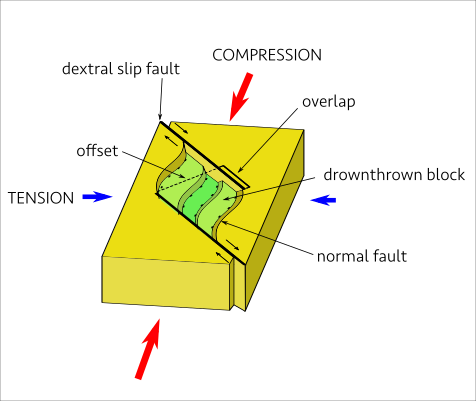
\includegraphics[width =\textwidth]{images/maps-of-mig/faultblock.png}}
\caption{A simplified block diagram showing development of a pull apart basin. Redrawn from \citet{WU20091608}}
\label{fig:fault}
\end{figure}

\begin{citemize}
\item Dinaric reverse thrusting within the Eocene (56Ma-33Ma BP). Reverse faults with orientations NW-SE orientations develop  \citep{castellarin2000neo}.
\item South Alpine thrusting transport of the Mesozoic carbonate platforms which form the \passage{Julian Alps} as described by \citet{placer1998contribution} and \citet{buser1986tolmavc} from possibly mid-Oligocene to mid-Miocene. This resulted in the various south verging overthrusts of the Zlatna and Julian nappes and the building of the topography like the Zelenacia ridge in the Triglav lakes valley. The resulting compressional tectonic structures are mostly E-W oriented \citep{castellarin2000neo}.
\item Neogene (Pliocene to Recent) dextral-slip faulting cross-cutting the Alpine generated topography, producing youthful landforms such as the Tolminka Springs Basin, continuing today, highlighted by earthquake activity \citep{vsmuc2009tectonic,cunningham2006application}. These NW-SE oriented faults cross-cut the previous Alpine structures\citep{grenerczy2005tectonic}.
\end{citemize}

 \begin{map*}[t!]
 \checkoddpage \ifoddpage \forcerectofloat \else \forceversofloat \fi
\centering
  \includegraphics[width=\textwidth]{"images/maps-of-mig/geological_map_with_symbols".png}
  
  \caption{Geological map of the Tolmin Area, modified after \citet{buser1986tolmavc}}
  \label{map:mapofgeology}
 \end{map*}

\section{Landscape development and controls}
\subsection{Lithology}
\label{par:lithology}
\marginnote{Lithology is described as summary of the gross characteristics of a rock}

\passage{Tolminski Migovec} is mainly formed by a sequence of massive to well-bedded (1-3m) pure grey to buff limestones with patches of dolomite \citep{buser1986tolmavc} belonging to the Dachstein formation (in Slovene 'Dachteinski apnenec'), which derives its name from the Dachstein massif near Salzburg, Austria \citep{ogorelec1996dachstein}. 


The rock formed during the Upper Triassic Norian to Rhaetian age (228 -101.3 Ma) and now forms the backbone the \passage[Calcareous Alps]{Southern Calcareous Alps} \citep{bosellini1974triassic} and crops out all over the \passage{Northern Calcareous Alps} \citep{fischer1975tidal,schwarzacher2005stratification}. It has given rise to spectacular landscapes spread over Southern Europe, from Hungary \citep{haas2004characteristics} to Sicily \citep{catalano1974ciclotemi}.
Its ubiquity has wide ranging implications for the palaeogeography of this region in Norian to Rhaetian times.

\begin{marginfigure}
\frame{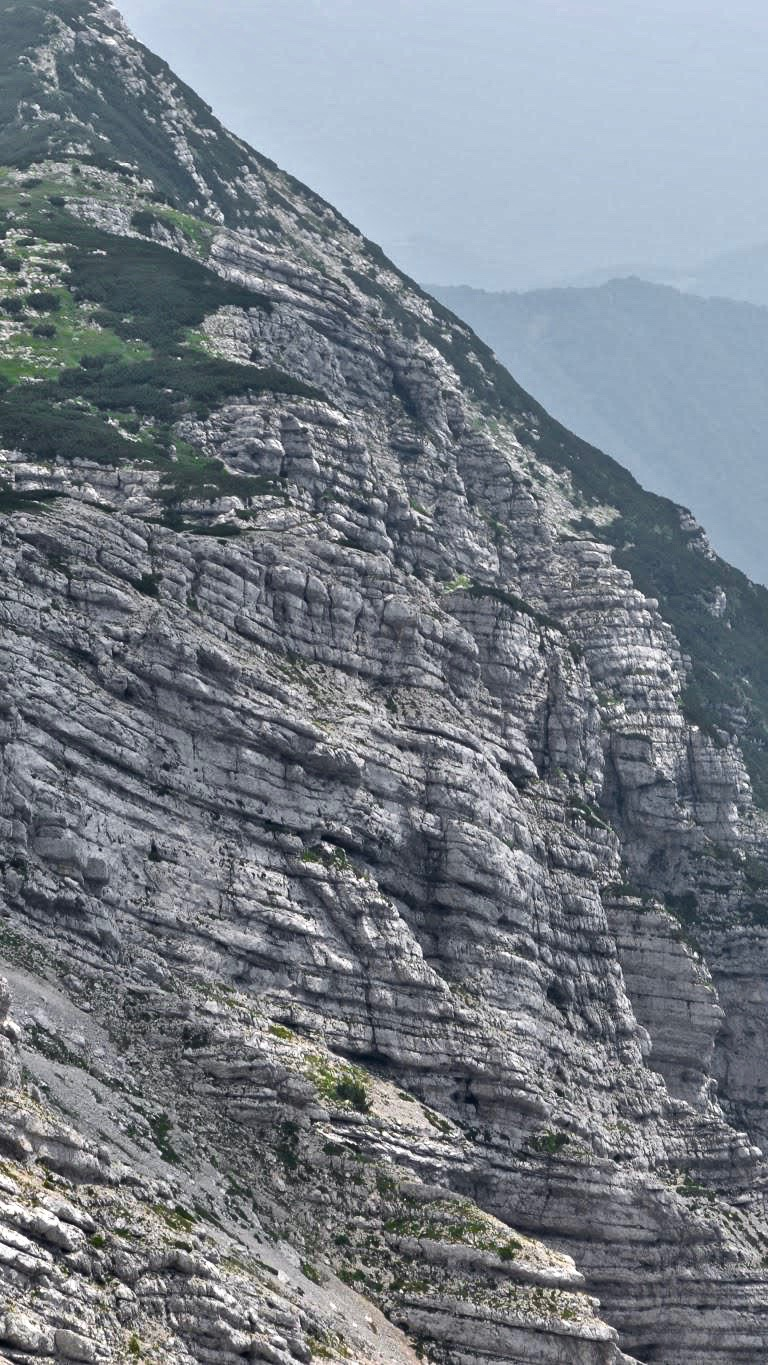
\includegraphics[width = \textwidth]{images/maps-of-mig/dachstein_limestone.jpg}}
\caption{The well bedded Dachstein limestone outcrops on the western cliffs of \passage{Tolminski Migovec} \pic{Rhys Tyers}}
\label{fig:dachstein}
\end{marginfigure}

The Dachstein limestone is typically well-bedded, nearly 1km thick and comprises both karst and palaeokarst phenomena \citep{ogorelec1996dachstein,haas2007characteristics}. Locally, it is underlain by the equally extensive Main Dolomite (in German 'Hauptdolomit'). The dachstein formation is thought to have been deposited in quiet but thriving shallow marine environments, where the accumulation of biogenic calcareous material was compensated by the steady sinking of the carbonate platform. 

The deposition of the Dachstein formation ended at the end of the Triassic (~200Ma BP) with the dislocation of the carbonate platform. Some regions stayed near the sea level (the so-called 'Julian High') while others were periodically drowned, leading to the deposition of carbonatic mudstones and shales within the limestone sequence within the Jurassic and Cretaceous \citep{vsmuc2010jurassic}; they are shown on \fref{fig:limestones and marls}.





\begin{marginfigure}
\checkoddpage \ifoddpage \forcerectofloat \else \forceversofloat \fi
\centering
 \frame{\includegraphics[width=\linewidth]{"images/maps-of-mig/marls_limestone".jpg}} 
 \caption{An example of the Jurassic marl and limestone succession, which is heavily faulted \pic{Tanguy Racine}, on the \protect\passage{Slovenska Geolo\v{s}ka Pot}}
 \label{fig:limestones and marls}
\end{marginfigure}

Debate is ongoing as to the origin of the cyclic pattern of the limestone beds often called \emph{Lofer cyclothems} --- so named after the Lofer locality in Austria where they were first described. 
These cyclothems were identified and interpreted by \citet{fisher1964lofer} as cyclic sequences tracking deepening upwards depositional environments.
The idealised cyclothem model shows three groups A, B, C corresponding to  subaerial, tidal and subtidal deposition environments respectively.  

This is demonstrated by palaeokarst solution vugs, the presence of argillaceous --- here terrestrially derived --- and often iron oxide rich residues and evidence of subaerial weathering, even palaeokarst in Group A.

Group B is often characterised by the presence of dessication cracks, partial dolomitisation; it is often laterally discontinuous, with variable thicknesses (5-155cm).

Group C, often the most abundant, comprises wackestones (rich in carbonatic mud) and packstones (dominated by biogenic fragments).


Often, the measured sections differ from the ideal model by the absence of certain members of the sequence. Indeed compared with the Dachstein limestones deposited in the Dinaric range, the limestones of the Krn area show more numerous and more pronounced periods of emersion \citep{ogorelec1996dachstein}.

 With some authors favouring local tectonic control as a causal mechanism  for relative changes in sea level \citep{goldhammer1990depositional,enos1998lofer}, others \citep{fisher1964lofer,balog1997shallow,haas2004characteristics,doi:10.1130/G21578.1}, prefer orbitally forced environmental fluctuations such as \emph{Milankovitch cycles} which result from periodic fluctuations in solar insolation linked with the Earth's \emph{precession}, \emph{tilt} and \emph{ellipticity} cycles. 

 \subsection{Glacial landforms}
 \citet{bavec2004late} used a combination of geological mapping and dating the identified glacial deposits in order to constrain the extent of late Quaternary glaciation in the upper So\v{c}a valley, which is relevant to the Tolmin area.

 Most notably, they find no clearly expressed glacial geomorphic features downstream of the town of Bovec; on the contrary, all landforms such as end moraines or glacial cirques are limited to the high reaches on the valleys. 

Locally, the bowl shaped hanging valley between the \passage{Migovec Plateau} and \passage{Vhr Nad \v{S}krbino} is one example of glacial cirque. Notably, the high resolution mapping of \citet{cunningham2006application} could not find any signes of side or -end moraine, nor any other glacially derived deposits within the \passage{Tolminka springs} basin and interpreted the sheer walls near \passage{Polog} as segments of the Ravne fault in a pull-apart basin. 
This is consistent with the view of \citet{vsmuc2009tectonic} on the relative primacy of tectonics over glacial processes on landscape building in the \passage{Triglav} area.

 \subsection{Karst landscape}
Karst terrain arises from the combination of high rock solubility and well developed secondary fracture porosity \citep{ford2013karst}. 

Such terrains exhibit several key features: fluted outcrops, sinks, caves, springs, blind valleys etc... It is the present of an unusual hydrology which dictates the development of 'karstic landscapes'. 

These landforms are generated by the dissolution of rock along natural subterranean pathways provided by geological features (joint, bedding planes, faults), the principles of which have been described by \citet{dreybrodt1996principles}, under several numerical models.

\begin{marginfigure}
\frame{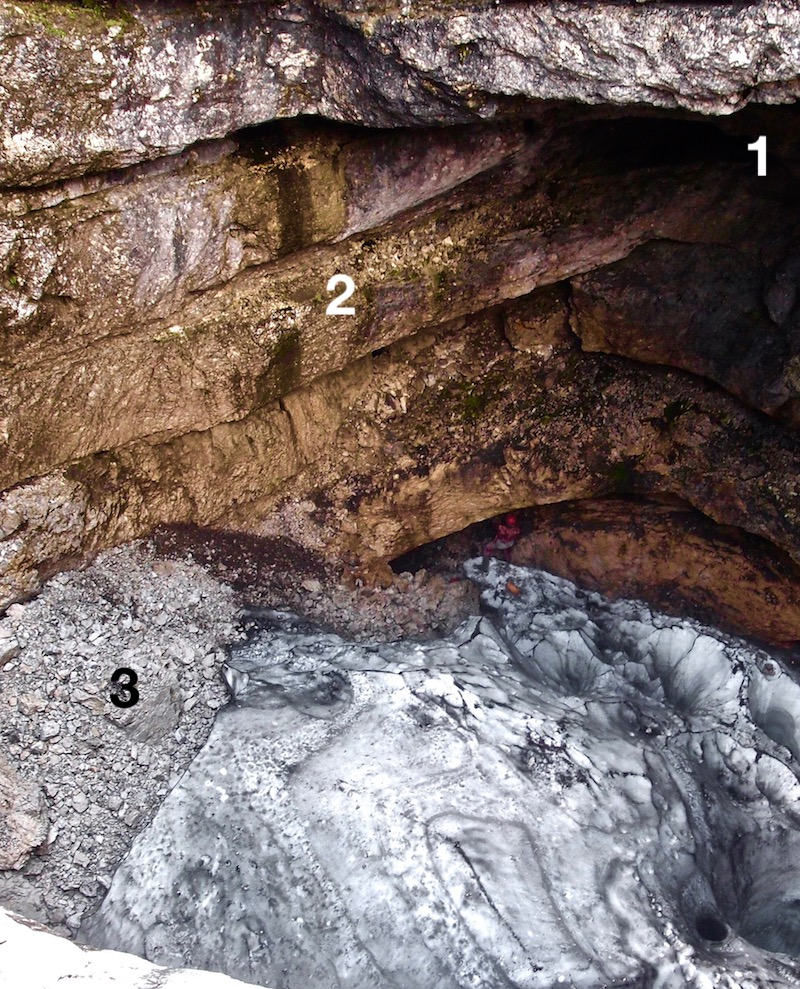
\includegraphics[width = \textwidth]{images/maps-of-mig/CeciliaKan_pothole_crop.jpg}}
\caption{The typical karst terrain of Migovec shows the interplay between 1) dissolution and abandonment of phreatic tubes 2) well developed planar porosity --- here bedding planes and fractures 3) freeze-thaw action leading to the formation of widespread scree talus \pic{Cecilia Kan}}
\label{fig:shaft}
\end{marginfigure}

It is now commonplace to think of inception horizons \citep{lowe1997carbonate} as promoting early cavern development and governing the maturation of a karst system. Soluble rocks with well developed primary or secondary porosities tend to support excellent karst. It comes as no surprise then that the well-bedded, often jointed and heavily faulted Dachstein limestones of Migovec exhibit most of the staples of alpine karst.

The development of karst is termed either \emph{eogenetic}, \emph{mesogenetic} or \emph{telogenetic} according to the following rules:
\begin{citemize}
\item dissolution of the host rock coeval with or immediately following its deposition and lithification is eogenetic karst 
\item dissolution of the rock by hypogene (deep seated) fluids as it is buried, is termed mesogenetic karst
\item dissolution of the rock by weakly acidic rainwater when the rock mass is made available by uplift is term telogenetic karst
\end{citemize}

The karst of \passage{Tolminski Migovec} shows both aspect of eogenetic karst such as solution vugs within \emph{Lofer cyclothems}, which developed during deposition and more significantly, telogenetic karst, which produced the many kilometres of enterable caves within the mountain.

The surface of the \passage{Migovec Plateau} is famously riddled with shakeholes and dolines. A cursory inspection of a topographic map shows that a majority of these 10-30m deep shakeholes are aligned with the dominant tectonic structures within the Migovec area (namely NNW to SSE lineaments). 

\begin{marginfigure}
\frame{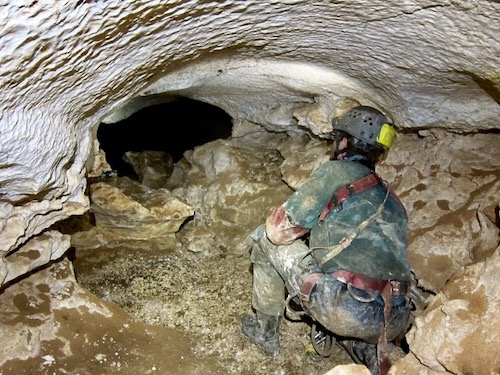
\includegraphics[width = \textwidth]{images/2016/tanguy-dvu-2016/jarv_buckwheat__1_.jpg}}
\caption{The above photograph demonstrates the various stages of cave development: the ellipical ceiling of the passage near \passage{Déjà Vu} junction is phreatic in origin. The sinuous rift below, as well as the mud and gravel deposits are vadose in origin \pic{Jarvist Frost}}
\label{fig:dachstein}
\end{marginfigure}

\section{The karst aquifer of Migovec} 
The karst aquifer is divided into two main zones: \begin{citemize} 
\item the \emph{phreatic} zone, situated below the water table, which consists of a network of water-filled conduits, planes or matrix under hydrostatic pressure. The largest phreatic tunnels are accessible to divers, either from within the cave (at siphons or 'sumps') or a springs, where the water finishes its underground course. 
\item the \emph{vadose} zone, situated above the water table, which consists of dry abandoned passages (fossil part of the cave) and/or deeply incised stream canyons or waterfall shaft series (active part of the cave). These passages are accessible to non-diver speleologists and often contain sediment banks or \emph{speleothems}. All are modified by the mechanical breakdown of the cave roofs, which can generate large underground chambers or caverns or block the continuation at \emph{boulder chokes}. 
\end{citemize}

The thickness of the vadose zone on Migovec, that is the elevation difference between the high entrances on the \passage{Plateau} and the sump levels, is about 900-1000m. The type of recharge present is autogenic diffuse (\citep{ford2013karst} which means that rainwater falls directly on the karstic catchment, collects within the innumerable fissures on the surface into small underground streams. These cascade down over 15 identified shaft and canyon series (but there are probably more), often disappearing down immature and impassable underground canyons. 

Over the course of 40 years of exploration, we have not found a master streamway, that is to say, a collector underground stream ending in a sump, whose resurgence is known \citep{hm1}. Rather, we have followed the disparate streams to at five different sumps located each within 30m of 890m asl. Other shallower siphons within the System are called 'perched'  as they are presumably the sign of a local watertable (e.g. \passage{Red Cow}: 1046m, \passage{True Adventures}: 975m, or even \passage{Terminus}: 1465m).

\begin{figure*}[t!]
 \checkoddpage \ifoddpage \forcerectofloat \else \forceversofloat \fi
\centering
\frame{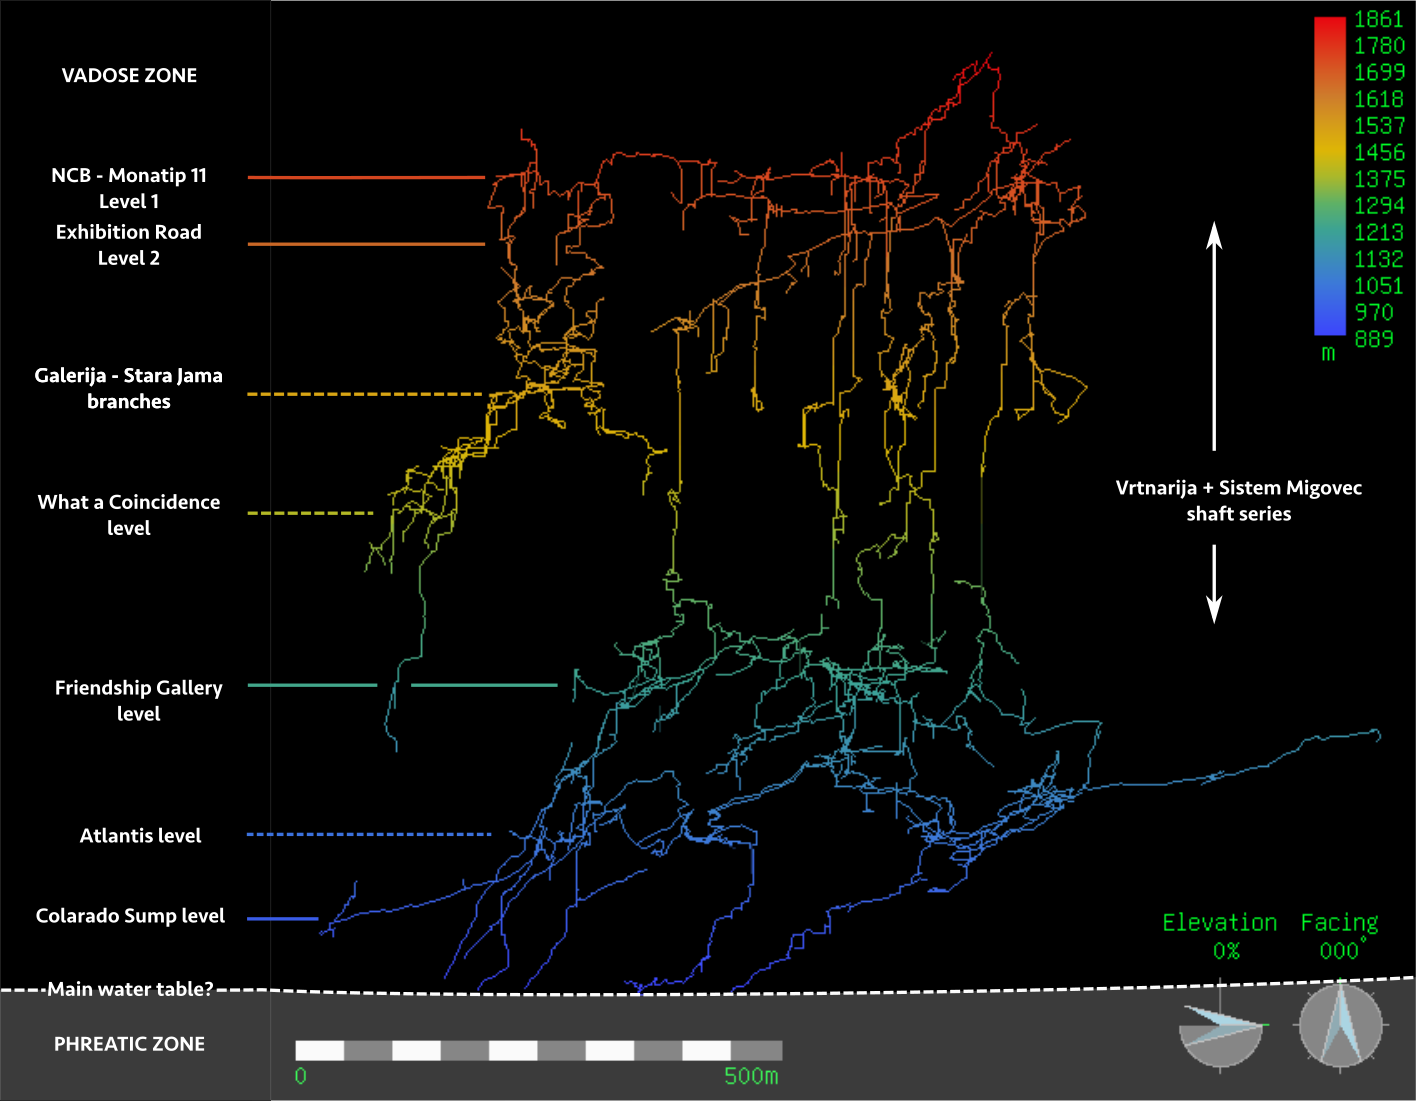
\includegraphics[width = \linewidth]{images/maps-of-mig/mig_aquifer.png}}
\caption{E-W projection of \protect\passage{Sistem Migovec} (2017) produced on \emph{Aven} software. Solid lines denote laterally continuous (>500m) horizontal passages of phreatic origin. Steepled lines denote more local horizontal passages of phreatic origin} \label{fig:ew projection}
\end{figure*}


\begin{pagefigure}
\checkoddpage \ifoddpage \forcerectofloat \else \forceversofloat \fi


\begin{subfigure}{\linewidth}
\centering
 \includegraphics[width=0.6\linewidth]{"images/maps-of-mig/rose_diagram".png}
\caption{}
 \label{fig:rose diagram}
 \end{subfigure}
 \vspace{3mm}
\begin{subfigure}{\linewidth}
\centering
 \includegraphics[width=0.6\linewidth]{"images/maps-of-mig/rose diagram 2".png}
 \label{fig:rose diagram 2}
 \caption{}
 \end{subfigure}
 
  \caption{A rose diagram depicting the azimuth ($\phi$) of cave passages. This was extracted from a .3d file produced on Survex, where  $n$ is the number of stations, $\theta$ is the inclination angle and the radial grid is the percentage fraction of passages falling in a specific orientation \emph{(a)} $n=5084$, $\theta <45°$ and \emph{(b)} $n=912$, $\theta \ge 45 \textdegree$. Each sector is 10\textdegree wide. Bin colour shows passage length distribution}
\end{pagefigure}

Reaching the 'water table' often occurs when the underground course of the water hits a lithological or tectonic boundary. In the case Migovec, it is probable that the contact between the Zlatna overthrust and the underlying Krn nappe, whose topmost rocks are relatively insoluble marls, will provide a benchmark for the watertable. It is curious to note however, that the five deep sumps occur above this impervious horizon - it means the sump level is likely the contact with a dolomitic body, which leaves open the possibility for further depth development. 

Imperial College Caving Club have attempted to trace the water from \passage{Sistem Migovec} \citep{hm1} to the \passage{Tolminka}, \passage{Zadla\v{z}\v{c}ica} and \passage{Sava} rivers.
 
 
 \subsection{Structural control of cave passage orientation}
 \paragraph{Azimuth of horizontal galleries}
 Horizontal sections of passage come under the name of \emph{galleries}: they are dry, fossil tubes which were enlarged when they were under the water table, and thus were part of the phreatic zone. Their orientation is guided by the intersection of bedding planes (near horizontal) and vertical joints and faults. They have a characteristic elliptical cross-section, which can be obscured by mechanical failure of the ceilings. Sometimes, sediment banks and speleothems are present (\fref{fig:atlantis}, \fref{fig:leprechaun}).

Under the assumption that survey legs are `optimised' \sidenote{`optimised' in that they are the longest possible given passage geometry. This is almost always valid for two reasons: 1) stations are chosen to reduced the survey workload inside the cave; 2) excessive 'bouncing off the walls' adds artificial length to the cave and is therefore frowned upon} the orientation of near horizontal cave, and in particular that of long stretches of rectilinear passage appears to be non-random. 

While short survey legs (<$4m$), which are typical of short, twisting complex passage or breakdown are regularly distributed within the azimuth space, long survey legs >$8m$, and by extension long rectilinear cave passage are significantly more numerous in the $145-195\textdegree  \pmod{180\textdegree}$  sectors and to a lesser degree within the $35-55\textdegree   \pmod{180\textdegree }$ sector (\fref{fig:rose diagram}).

The orientation is therefore likely dictated by a set of planar discontinuities (joints or fractures) aligned with the general direction NNW-SSE, and a minor set in direction NE-SW \fref{fig:rose diagram}. This conclusion is in accord with in-cave observations \citep{hm1}  and previous surface mapping \citep{buser1986tolmavc} . Indeed many, if not all of the strike-slip and normal faults whose planes are chiefly vertical are oriented in a NNW-SSE direction and to a lesser extent in a NE-SW. (\fref{map:mapofgeology}).

At depth this also supported by observations on several abandoned phreatic routes and low gradient vadose canyons:
 
\begin{citemize} 
\item \passage{Minotaur Rift} (\fref{fig:minotaur_rift})
\item \passage{Amazing Grace} and \passage{Atlantis}  (\fref{fig:atlantis})
 \item \passage{Push Your Luck} - \passage{Agartha} (\fref{map:pushyourluck})
 \item \passage{Highway 32} (\fref{fig:highway32})
 \end{citemize} 

These passages are useful markers of the water table position in the past


\paragraph{Pitch series development}
 Vertical sections of passage are called \emph{pitch}, \emph{drop}, \emph{shaft}, \emph{pit} or \emph{pot}; in Slovene \emph{brezno}. 
 Several pitches in a row make a \emph{series}. Some ~15 pitch series in Migovec are over 200m deep, and most are over 400m.
Some of the deepest shafts within the system include \passage{Silos} (113m), \passage{Plopzilla} (105m), \passage{Happy Monday} (81m). They are commonly over 10m in diameter at the base. 

S 




	\section{Building the Survey of the Migovec Cave System}

\begin{quote}
"By 1996, the importance of an accurate and complete survey was apparent to all - being instrumental  in finding the connection and making a cave system" --- James 'Tetley' Hooper, The Hollow Mountain, 2007. 
\end{quote}

The following article is an extension and update  on 'The Survey Project' published in the previous Hollow Mountain volume. It aims to describe the process of survey and map making we have followed from 2013 onwards. Each end of expedition has seen a different party taking charge to collate drawings and curate the entered data before delivering a plan survey and extended elevation detailing the newest findings. To reflect this, we include each year's survey at the end of the relevant chapter.

\begin{marginfigure}
\checkoddpage \ifoddpage \forcerectofloat \else \forceversofloat \fi
\centering
 \frame{\includegraphics[width=\linewidth]{"images/survey/compasses-jarv".jpg}} 
 \caption{Suunto instruments and their protective caves are inspected prior to leaving on expedition ---Jarvist Frost}
 \label{compass}
\end{marginfigure}

\begin{marginfigure}
\checkoddpage \ifoddpage \forcerectofloat \else \forceversofloat \fi
\centering
 \frame{\includegraphics[width=\linewidth]{"images/survey/jarv-pss".jpg}} 
 \caption{A Permanent Survey Station is left at one of the Junctions in the cave, here detailing the updates at the pushing fronts ---Jarvist Frost}
 \label{PSS}
\end{marginfigure}


\subsection{Data collection and storage}
The skeleton of the survey project is the \emph{main line}, a 3D model which links several thousand nodes or \emph{stations}. Each station is linked to one or several neighbours by a distance, inclination angle and azimuth. These quantities are measured in the cave with the aid of tape measure or laster range-finder, inclinometer and compass respectively. Additionally, splay legs in the plane normal to line of sight are measured: they indicate the distance to cave passage walls from the survey station of interest. \emph{Permanent Survey Stations} or PSS's are those stations where an easily found physical landmark (such as a cairn), together with descriptive, waterproof paper label exists inside the cave: these are used to 'tie in' new strings of the survey.

It is usual for a pair of cavers to conduct the survey by assigning the data logging to one, and instrument reading to the other. By calling out the measurements in a clear, well detached and unambiguous manner, we are able to minimise the number of typographical errors. The data is entered in pencil on waterproof logbooks (A6 format) and details for each line:

\begin{citemize}
\item direction of sighting (i.e.: from station 1 to station 2 or vice-versa)
\item distance (XX – YY)
\item azimuth (XXX)
\item inclination(±YY)
\item left, right, up, down \emph{splays}
\item direction of sighting (i.e.: from station 1 to station 2 or vice-versa)
\end{citemize}

Finally, blank pages are ideal for drawing small surveys of the newly discovered cave passage, writing additional notes, logging which survey stations.

Back on the surface, it is necessary to back up the collected measurements and 'enter' the data digitally before it can be processed. Usually, the relevant pages of the survey books are photographed and filed in resealable plastic pouches and stored in a shockproof pelicase together with the bivi computer. 

The next step, often the same evening (or morning) a group has come back to the surface, the notes are read and entered on a template text file. The file, which includes more information such as the names of the surveying party, the specific roles (ie: books or intruments), PSS location or the number of pages, is then processed by the Survex software (developed by Olly Betts from Cambridge University). By reading back the data, more typographical errors are avoided. In this step, we also specify where a specific string of survey legs should be tied into the master system. 

\begin{marginfigure}
\checkoddpage \ifoddpage \forcerectofloat \else \forceversofloat \fi
\centering
 \frame{\includegraphics[width=\linewidth]{"images/survey/jarv-survey-notes".jpg}} 
 \caption{A excerpt of a exploration notebook after the measurements are pencilled in ---Jarvist Frost}
 \label{notebook}
\end{marginfigure}

Over the years, we have divided the cave into different systems (\emph{Vrtnarija, Monatip} etc,…)  and regions (\emph{Apollo, Stuck in Paradise} etc,…), which is reflected in the hierarchy of nested folders, all of which ultimately contain specific, survex-compatible \emph{.svx} files.


 \begin{figure*}[t!]
 \checkoddpage \ifoddpage \forcerectofloat \else \forceversofloat \fi
 \centering
 \begin{tikzpicture}
\node [table] (box){%
    \begin{minipage}{\textwidth}
    \begin{multicols}{2}
    \centering
\begin{verbatim}
;Apple Crumble
;Window off Povezava pitch

;Date: 24/07/17
;Instruments: James Wilson
;Book: Tanguy Racine

;Data entered by Tanguy Racine 25/07/17

;data normal bcra grade 5
;from	to	tape	comp	clino

;data on 3 pages
*begin apple_crumble
;PAGE 1/3
2	1	4.04	165	-24
3	2	5.90	134	-22
4	2	2.83	207	-09
…

;NOTES
;STN 1 IS PSS at junction of muddy crawls
;STN8 is cairn in TTT branch
;STN 9 IS PSS
;STN 7 is PSS
…

*end apple_crumble
*equate apple_crumble.26 pov.11
\end{verbatim}
\end{multicols}
  \end{minipage}
  };
\node[tabletitle, right=10pt] at (box.north west) {A typical survex file};
\end{tikzpicture}
\end{figure*}



\subsection{Processing and displays}
When the data is processed on the terminal,  \begin{verbatim} cavern pathto/asurvexfile.svx \end{verbatim} 

each \emph{station} is prefixed by the name of the enclosing file or folder, therefore station 4 of \emph{stranglehold} becomes stranglehold.4. This enables the station to be called and equated to another node to tie the survey together. 

Survex begins its work with a fixed point or origin and assigns it cartesian coordinates of  $(0;0;0)$. All other station coordinates in the survey file are calculated in series, relative to the origin. In case there is an indicated loop, survex distributes the error evenly across all the measured legs in the loop and this is recorded in an error log. Each individual file is processed separately before it is appended to a master, regional file such as \emph{Primadona.svx}. There, a PSS from a previous survey can be equated to a station in the new file, and a new process begins:
\begin{itemize}
\item Calculating and redistributing the errors on trans-file loops when a major connection is made
\item Correcting for each year's magnetic declination variations, (several degrees for just a decade difference)
\item checking splays and flagging up re-surveyed legs 
\end{itemize}


The output of the processing is an \emph{.3d} file displayed in \emph{Aven} software. The end product is essentially a line mesh coloured by either depth, date of exploration or loop closure error; this can be rotated 360° in the horizontal plane, 180° from top-down to bottom-up in a vertical plane. Given a surface elevation model, one can also manually check the distance from a node to the surface, or from node to node. One advantage of processing the survey datasets very early on is that the sorts of queries such as 'how close are these two passages' determine the orientation of exploration during the expedition; answering them right away enables connection efforts and fuel most of the heated evening discussions about where to explore next.

\begin{marginfigure}
\checkoddpage \ifoddpage \forcerectofloat \else \forceversofloat \fi
\centering
 \frame{\includegraphics[width=\linewidth]{"images/survey/surveying_colony".jpg}} 
 \caption{Will Scott surveying the climb into \emph{Colony}, using compass and clinometer ---Tanguy Racine}
 \label{surveying colony}
\end{marginfigure}

The main deliverable from \emph{Aven} is undoubtedly the main line; the plan view projection thereof can exported into a vector graphics software like \emph{Inkscape}. The elevation view is more intuitive because Sistem Migovec is predominantly a vertical cave system; however, a simple projection is of limited use when it comes to drawing cave passage walls around the main line. The overlapping vertical shaft series blur into one, and labelling each passage becomes an issue. Finally, the projection distorts most the horizontal length of passages near parallel with the line of sight.

To overcome this problem, we produce an \emph{extended elevation}, where starting from a reference point ( the cave entrance of \emph{Vrtnarija} in our case), the survey legs are unfolded into one vertical plane. The distance from station to station, and inclination angle between remain unchanged, only the azimuth is changed to either N, or S (left or right on the plane). 

The major consequence of this operation is that the distance between non-adjacent nodes is no longer reflected on the visualisation software. As a corollary, long or complex loops are sometimes broken and completely unfolded. To meet the needs of the user, whether it is greater topological accuracy or the aesthetically pleasing distribution of passages on a page, it is possible to write instructions for the extension process and force a series of passage in a certain direction.

 \begin{marginfigure}
 \checkoddpage \ifoddpage \forcerectofloat \else \forceversofloat \fi
 \centering
 \begin{tikzpicture}
\node [table] (box){%
    \begin{minipage}{\textwidth}
\begin{verbatim}
;Organising Fenestrator branch
*eright prim.fenestrator.9 
*eleft prim.battery_flattery.1
*eright prim.battery_flattery.10
*eleft prim.alabaster.5
*eleft prim.sweet_baby_jesus.24
*eright prim.sweet_baby_jesus.22
\end{verbatim}
  \end{minipage}
  };
\node[tabletitle, right=10pt] at (box.north west) {Instructions};
\end{tikzpicture}
\end{marginfigure}

This is done via the following terminal command:
\begin{verbatim}
/Applications/survex/extend --specfile=instructions.dat 
   pathto/Avenfile.3d  pathto/extendedAvenfile.3d
\end{verbatim}

creating a new, \emph{Aven} compatible .3d file, which can in turn be exported to a vector graphics software.

The instructions text file gets longer, and more complicated every year: it is the result of trial and error and a mixture of personal taste for where a passage should be and practical drawing considerations. 

\begin{figure*}[t!]
 \checkoddpage \ifoddpage \forcerectofloat \else \forceversofloat \fi
\centering
\frame{\includegraphics[width=\textwidth]{"images/survey/projection".png}}
\caption{projections of the line survey}
\label{projection}
\end{figure*}


\subsection{Making the final maps}
With a Vector Graphics Software package, it is possible to import the main line survey.The cave outline, passage walls, presence of water cascades can then be drawn around the skeleton to convey an idea of scale for the various caverns and pitches inside the cave.

By working with a cascade of well-organised layers, it is possible to hide or lock off several regions of the cave; each new addition comes under a different year label or region file. This drawing of the cave occurs after the end of an expedition, when all the grade 1 surveys drawn inside the cave or inside the bivi logbook are brought together at a survey meeting in the UK.

All newly added passage is duly annotated and labelled on plan and elevation and finally a scaled map and elevation of the cave system is submitted to the Slovene government in order to update it's \emph{kataster} database. A copy can be found on the Imperial College website.

\subsection{Geographical Information Systems and the survey}


	\section{Mig colloquialisms}

The following is a necessary update on the Migovec vernacular first published in the Hollow Mountain \citep{hm1}. This particular dialect of caving linguo is alive and thriving. 



\begin{description}
\item[Cow] Dried milk powder.
\item [Clag] What clouds look from the inside when enveloping the moutain
\item [Comf] Soft comfortable material to sit or lie on e.g. squares of chopped karrimats
\item [McGowan] A  dwarf pine based sofa so called because it resembles a bodybag containing the eponymous caver
\item [Faff]  To laze, waste time or take part in pointless labour
\item [Ey-Ohh] All purpose non-descript salutation
\item [Twatty] Adjective used to describe sections of cave which are tight, annoying or unnecessarily awkward.
\item [Schonky] Blanket adjective to describe anything dodgy, dangerous or loose, especially in caves
\item [Vitaminski] Powdered vitamin  sugary fizzy drink (comes in blue, yellow, orange and green flavours).

\begin{description}
	\item [slushies] Vitaminski mixed with ice from M10 on a hot day
\end{description}

\item [Blue Cloud] Patch of blue sky on a day of unrelenting clag
\item [Sunset] Evening ritual of fortified mountain tea consumption
\item [Slop] The evening cooked meal to go on the carbohydrates.
\item [the Hydro] A lovely swimming location near the Hydroelectric scheme of Tolminske Ravne
\item [$2^{nd}$ aid] Pills for hypochondriacs
\item [Old Lag] \textbf{O}wn kit, \textbf{L}eader, \textbf{D}river and experienced member of ICCC aged 25+
\item [Lightning Alley] A strip of fairly flat grass located high up on the Plateau. Not for the faint hearted.
\item [M10] Don't fall down M10
\item [Plateau] Undulating surface of Tolminski Migovec, anything between the Kuk and Mig trig points
\item [Mig] our spiritual home
\item [Union/La\v{s}ko polemic] Argument about the various merits of the two available beers in Slovenia. \sidenote{They are from the same manufacturer}

\end{description}


%____________________________PART 2 - EXPLORATION OF MIGOVEC

	\begin{tcolorbox}
	\part{The exploration of the Migovec system between 2013-2017}
\end{tcolorbox}
	\backgroundsetup{	scale=1,
					color=black,
					opacity=1,
					angle=0,
					contents={%
  							\includegraphics[height=\paperheight]{images/backgrounds/Part-2-explorations.jpg}
  					}
	}
	
\BgThispage
%__________________________________ CHAPTERS
  	
	%2013 text
	\begin{tcolorbox}
	\chapter{2013 - Z Miga Na Kuk}
	\paragraph{`Z Miga Na Kuk'} was our first full expedition caving in the longest cave in Slovenia and what better place to begin. 

It was a highly successful 5-weeks of cave exploration on Migovec. Collectively JSPDT and ICCC cavers added another 1.8\,km of new cave passage to System Migovec (already the longest cave in Slovenia) bringing the total to an impressive 27.3\,km. We were also continuing to camp at `Camp \protect\passage{X-Ray}{}', 600 metres below the surface, and most cavers were spending multiple days underground here. 

We were quite comfortable at this depth and in fact all the findings in \passage{System Migovec} this year were at depths greater than -500\,m relative to the entrance.

\end{tcolorbox}
	\backgroundsetup{	scale=1,
					color=black,
					opacity=1,
					angle=0,
					contents={%
							  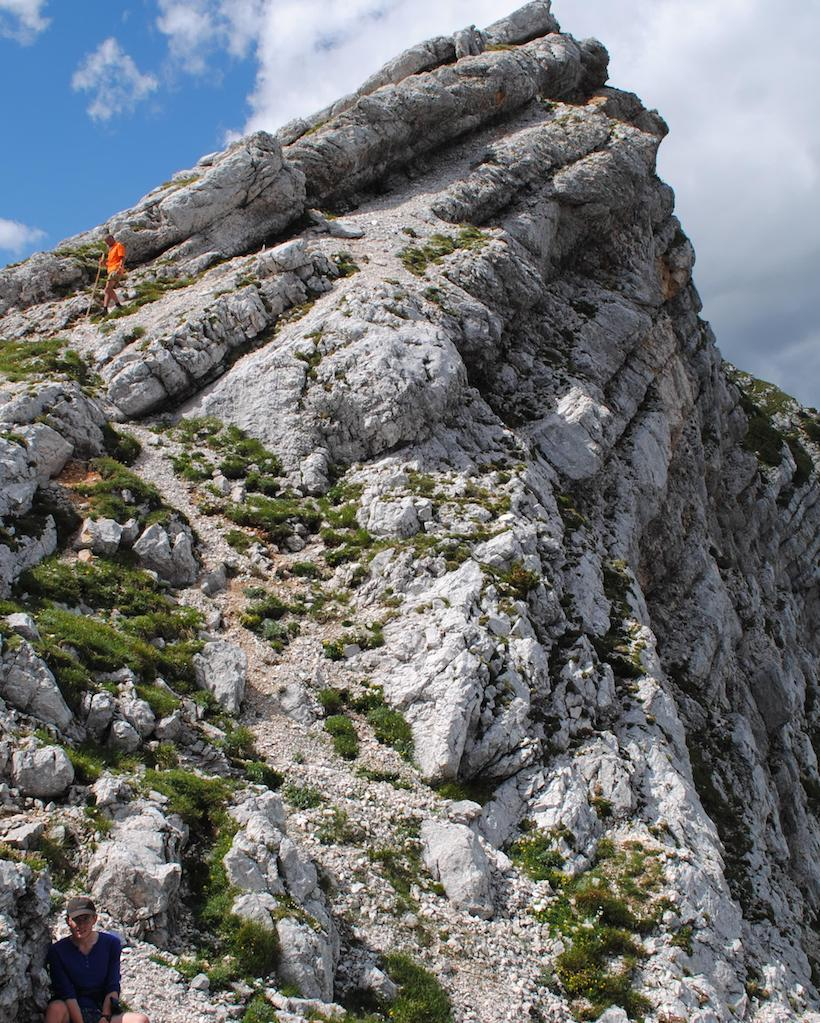
\includegraphics[height=\paperheight]{images/backgrounds/kuk-2013.jpg}
 					 }
	}
\BgThispage

	
\section{Exploring the longest cave in Slovenia}

We’d made a name for ourselves last year, connecting the ‘old’ \passage{System Migovec} with the newer \passage{Vrtnarija} (\passage{Gardeners’ World}) system and the pressure was on to perform again. We certainly couldn’t allow \passage{Postojna Jama} any chance of reusing their pre-2012 literature (now the ‘longest cave in the classic Karst’). 

\begin{marginfigure}
\includegraphics[width=\linewidth]{"images/2013/welcome-2013/clare_minestrone".jpg}
\caption{Inserting onself in short and worryingly small tubes was a staple of the pushing in the Atlantis extensions --- Rhys Tyers}
\label{clare_minestrone}
\end{marginfigure}

There was little debate over the year as to the plan. Leads abounded in Vrtanrija, and with so many still close to Friendship Gallery, we’d have been fools not to return to 'Camp \passage{X-ray}'. We’d been there since 2010 so the organisation and set up was slick. With good food (apart from the odd meths or petrol contaminated packet), bangin’ tunes (plus all the Blackadder audio one could hope for), and the warmest Jim-sized comf for sleeping in (though I’m pretty sure Jim doesn’t have a 1m long neck...) it was the perfect base for deep caving.

And deep caving there was! Close to camp \passage{Xanadu}, the unlikely find of last year, kept going! A pitch at the end of a grim muddy tube with a howling draught was finally dropped (after several attempts and a little bit of crying) into a superb horizontal level with multiple leads. Streamways, pitches, entertaining squeezes (and an epic traverse) this bit of cave has it all.

\begin{marginfigure}
\includegraphics[width=\linewidth]{"images/2013/welcome-2013/fiona_surface".jpg}
\caption{Surface exploration also entailed the pushing of small tubes. One of them broke through to a sizeable cave --- Rhys Tyers}
\label{fiona_surface}
\end{marginfigure}

At the end of \passage{Friendship Gallery} was '\passage{Yorkshire}'. The streamway was lengthened by several hundred meters despite the fact that all the pushing teams that visited this area were completely incompetent. Ending with a large chamber and a sump, an obvious sump bypass is blocked by one small boulder leaving a tantalising lead for 2014.

Deeper still, on the whispered advice of Jim, \passage{Balamory} was revisited. Lovely big pitches got deserving names (\passage{Clapton}, \passage{Bingo Granny}, \passage{Pick Your Poison}) and the lead was pushed and left going at a streamway at -850m! A second offshoot led to dry, sandy passage which eventually chokes but looks suspiciously similar to, and is heading straight for the end of...

\passage{Minestrone}! The Southern extensions of the cave were revisited. No big pitches, or stomping passage unfortunately. A terminating aven for \passage{Invictus} was found (\passage{RCC Passage of the Year}) and a bizarre upward spiralling tight crawl, \passage{Hash}, was pushed much further than it should’ve been. In the same area a sump, Lethe, was found at the end of \passage{Brezhno Slapov} but with tantalising opportunities for a bypass.

\begin{marginfigure}
\includegraphics[width=\linewidth]{"images/2013/welcome-2013/rhys_clare_bohin_by_kate".jpg}
\caption{Glorious weather on the surface enabled many scenic walks over the \protect\passage{Triglav National Park}. Here to \protect\passage{Zeleni Vhr} overlooking Lake \protect\passage{Bohin} --- Kate Smith}
\label{fiona_surface}
\end{marginfigure}

The weather up top was remarkably good for nearly the whole expedition so the surface was a frenzy of activity. An NPC contingent meticulously catalogued and pushed every possible hole on the Western side, noting the possibilities for further extension. One surface lead, '\passage{Jailbreak}', was pushed for over 100m. The activity was not all human as well. A thriving colony of yeast was set up and no, not in anyone’s socks. An attempt to brew beer in bivi resulted something that looked a bit like beer and gave you a hangover immediately. A great success.

	\section{Our Minds Were Full of Questions}
\margininbox{Atlantis}{
    \begin{itemize}
    \item Sam Page
    \item James `Tetley' Hooper
    \end{itemize}
}{\explo}
\label{sec:creature}

\paragraph{Sam 8.40am}

It had been my longest pushing trip to date, and my first time beyond \passage{Stuck in Paradise}. Our pushing target had been \passage[see|{Hash}]{\#}, in which we had great fun squeezing ourselves through the twisty-turny tunnels. Once we had reached a point at which we felt we could progress no further through the ever narrowing passage, we surveyed our way back, adding a small number of metres to the survey. Tetley was keen to check out some of the newly discovered cave nearby – particularly \passage{Atlantis} and its formations. Given our relative proximity to this area, I agreed to go along with this plan, although I think I was ready to return to camp already at this point.

\margininbox{Sam 5.40am}{Tet's gone all philosophical...}{\logbook}

We ventured down to \passage{Atlantis}, and without hanging about for too long, began the long trip back to camp. Our plan was slow-and-steady, with plenty of rest breaks. I was the first to arrive at \passage{Hawaii}, and sat down to catch my breath and have a drink. Something caught my eye, movement in the rocks. I looked down and there was an animal beside me! It was a kind of small, furry rodent, black with a long fluffy tail. At this point, Tetley was clambering over the rocks to join me. I anxiously asked him `Look at this - What is it?!', and when he noticed the animal, he gave a shriek. The animal then moved off and disappeared under some rocks and we did not see it again. This all happened within a short number of seconds. Our minds were full of questions. What was it? Where did it come from? How did it get to this bit of cave? How does this make us feel? 

\margininbox{Tetley 7.30pm}{Talking of Petzl, as a boy I read his tales of cave exploration, also the stories of \passage[super good French cave]{Dent de Crolles}, \passage[yet another eally great French cave]{PSM}, \passage[a superb French cave]{Gouffre Berger} etc. Looking now at the survey of our 25km system (hopefully now 30km+ if \passage{Primadona}/\passage{Monatip} has now connected in) it really is amazing, truly amazing, that we've a tale and a cave of similar magnitude!
I'm feeling sleepy again so I'll spare you my musing on love/relationships...}{\logbook}

Of course, our journey back to camp remained. Our discovery of the animal remained on our minds throughout. Assuming that it did not live in the cave (revolutionising science), it must have come from the surface. How then did it arrive at \passage{Hawaii}, somewhere which to the best of our knowledge was deep underground and far removed from any of the cave entrances? Probably given the length of our pushing trip and tiredness, our minds roamed to stranger explanations, of aliens or hallucinations or magic. More often, we just laughed at the peculiarity of our experience. 

We had camp to ourselves, and I seemingly slept for 17 hours(!). We decided against a third day of pushing, instead to make our way back to the surface. The concoction of thoughts surrounding the creature we found was intensified by the time we spent underground without seeing another person. We were desperate to be able to tell everyone about what we had seen, and to see if they believed us or not. Given that we saw the animal for such a short period of time, and me the longest of the two of us, it was easy to question if we really had seen such a thing. For the sake of our sanity, we decided that we had. 

\name{Sam Page}

\section{The Minds in Question}

Just back from our trip and I am ever so slightly broken...
More Importantly, WE ARE NOT ALONE! Me and Tetley saw a fucking animal at \passage{Hawaii}. It was some sort of mix between a rat and a squirrel, black with a long fluffy black tail. Something like this. 

After I sat down I turned my head an it was just there. My first reaction was to ask Tetley `What is \emph{that}?'; his first reaction was to scream as it moved and ran away. I probably watched it for around ten seconds before it disappeared. Where did it come from to end up at -800m!?! Does this mean there is an entrance somewhere around there. How could it get to where we were; it looked like it was moving well yet was spooked by us. We too were spooked by it. Surely it and more of its kind don't live down here with us? First action when back on the surface is to find out if such a creature exists.
P.S. Creature Theories
\begin{citemize}
\item 1. Saber brought it down in a cage and released it
\item 2. It came from outside
\item 3. Tetley and Sam had a mad hallucinogenic trip
\item 4. An alien invasion of \passage{Sys Mig}
\item 5. A creature to revolutionise all known biology - where does it get its light/food from???
\item 6. Magic
\end{citemize}

\begin{figure}[t!]
	\checkoddpage \ifoddpage \forcerectofloat \else \forceversofloat \fi
	\centering
	\frame{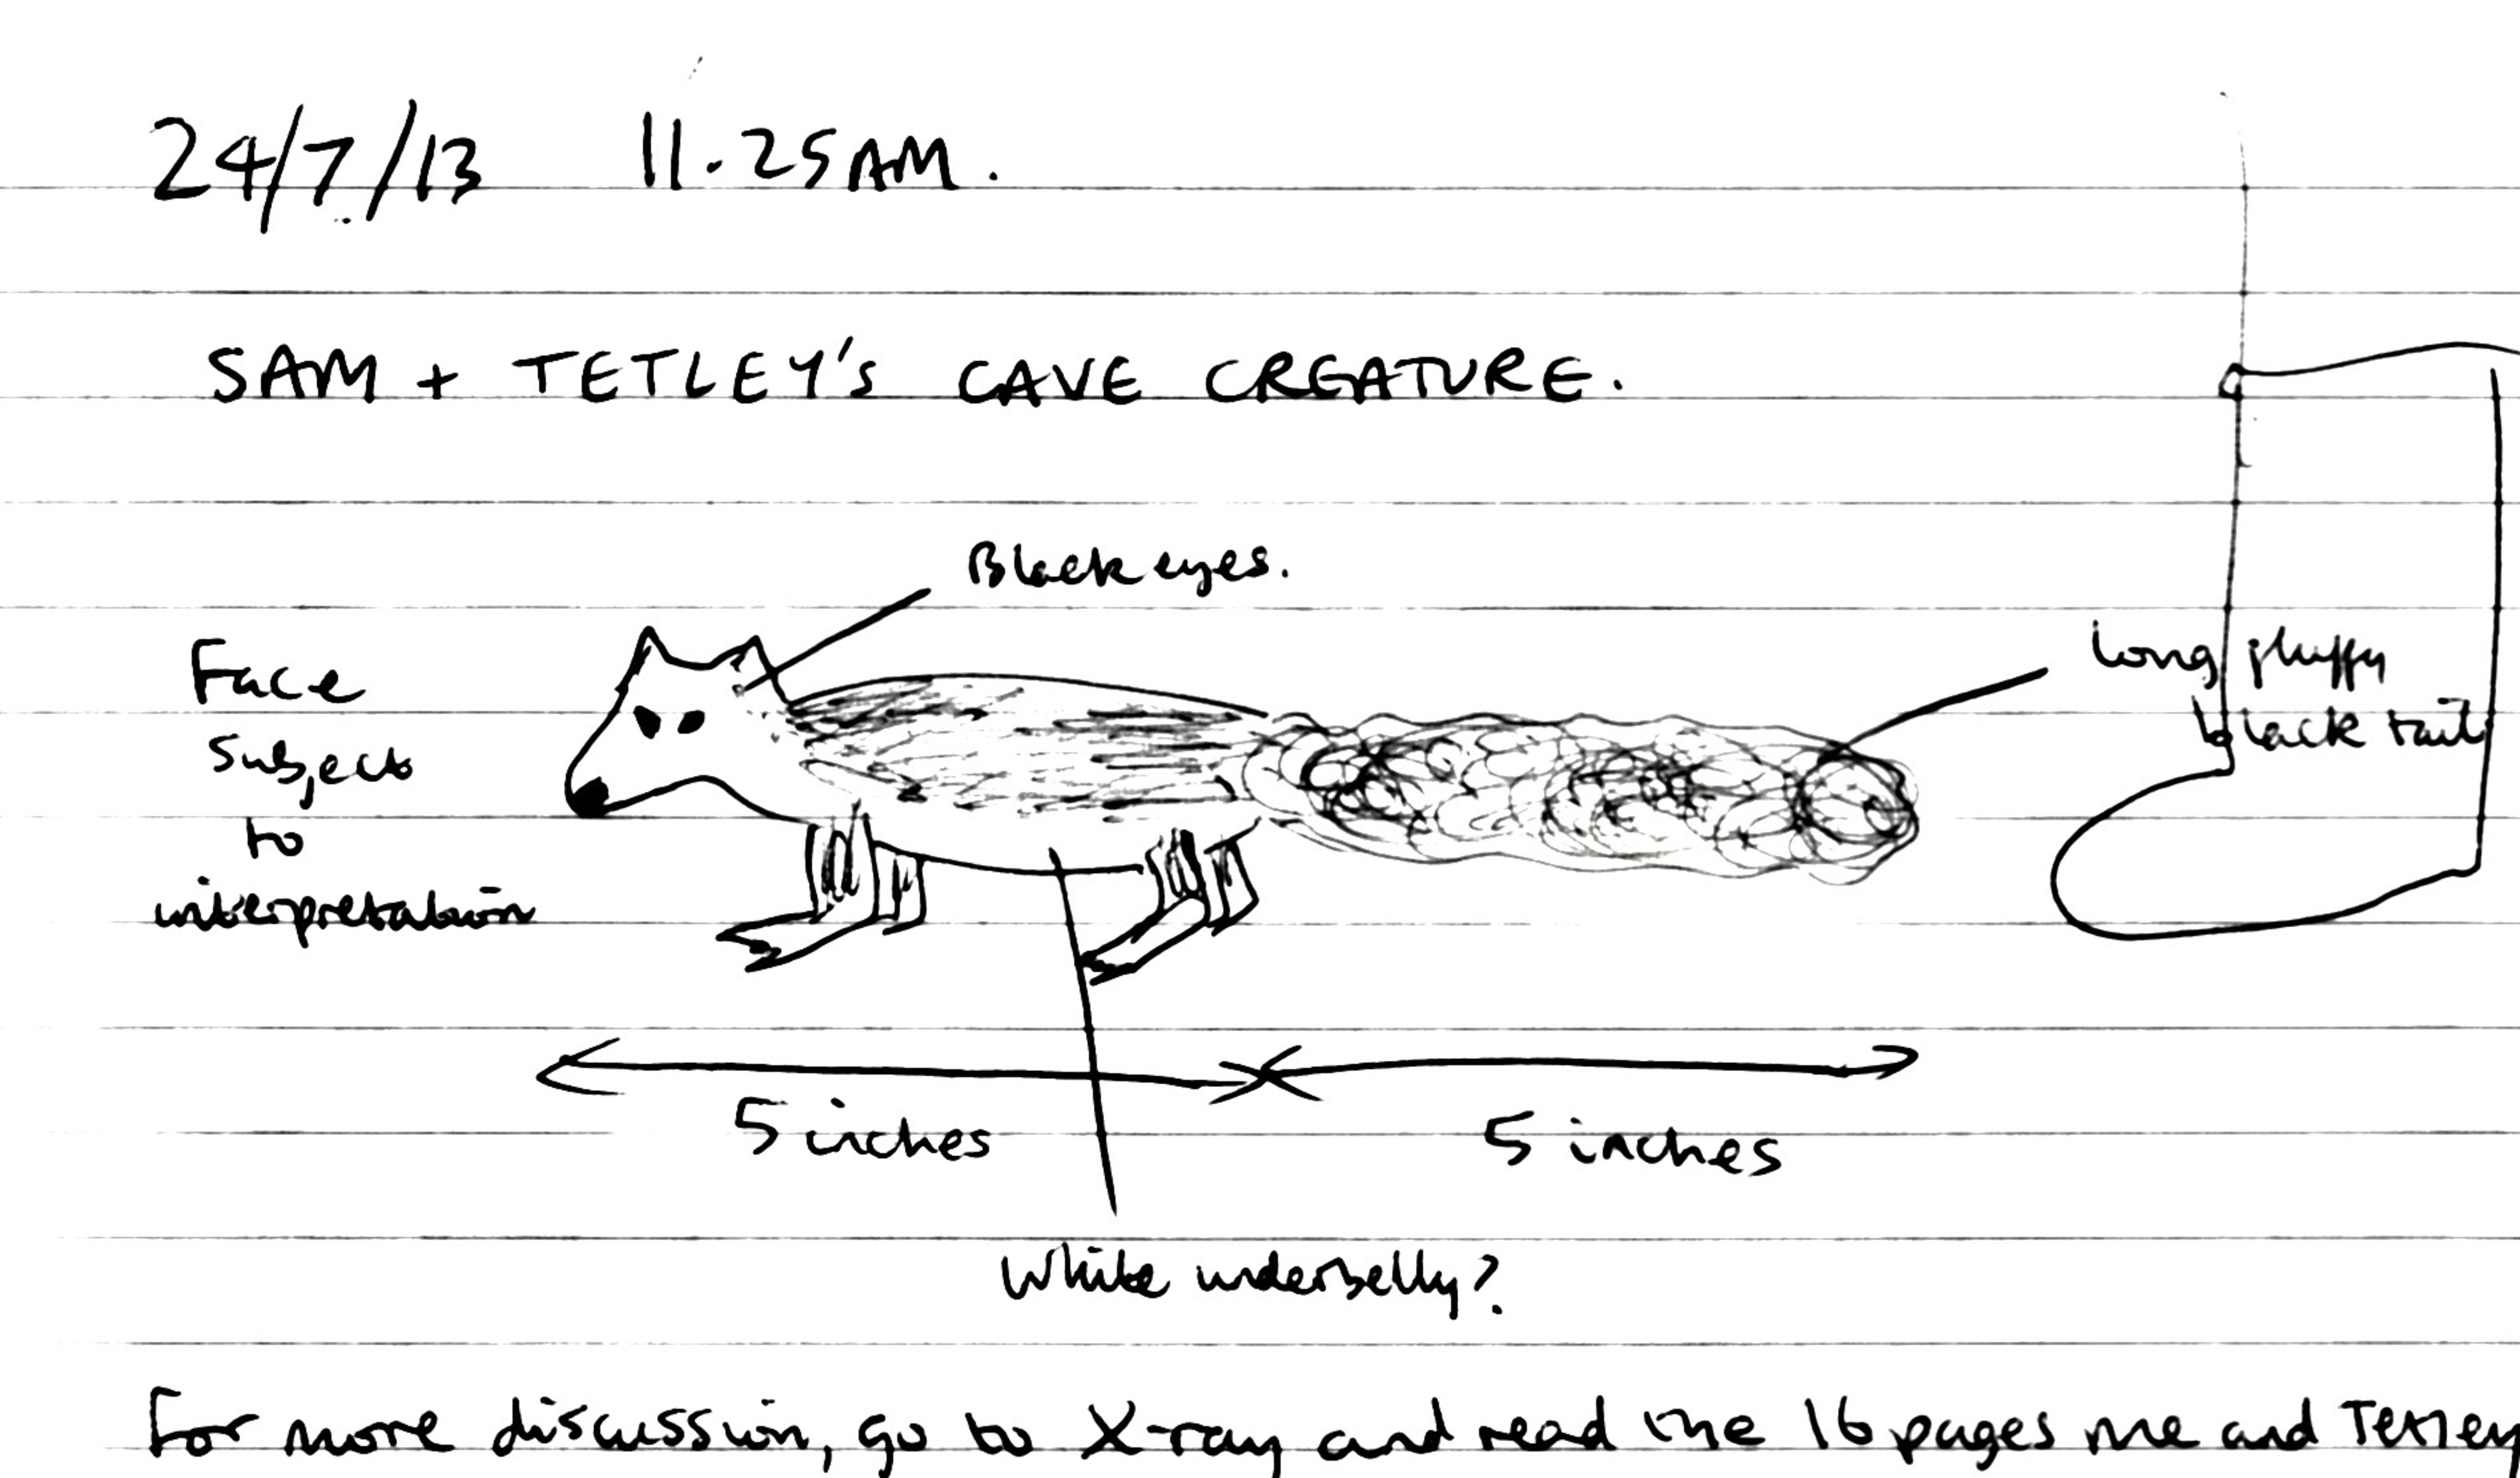
\includegraphics[width=\textwidth]{images/2013/tetley-sam-2013/creature.pdf}}
	\caption{The creature spotted by Sam and Tetley, drawn in the 2013 scanned logbook --- Sam Page}
	\label{the_creature}
\end{figure}


\paragraph{Tetley 7.30pm}

So our trip yesterday... a smooth journey down to \passage{Hawaii}. \passage{Stuck in Paradise} is much much better than when I first went down but still somewhat muddy and loose. Sam's first trip to this part of the cave. We had vitaminski tea and hot fish sandwiches. Went to push \passage{Hash}, added 25m (Sam described this earlier). The lead isn't great but it is still draughting and going. We then went to see the nice stal at \passage{Atlantis}, very pretty! Back to \passage{Hawaii} for tea...Sam was ahead of me and as I neared \passage{Hawaii} said, with I detected a slight anxious tone in his voice, `Tetley, Tetley look at this'. I was thinking maybe he was watching a spider or something...I approached and there to my surprise (to put it mildly) was a rat type creature. It moved! I screamed!

What! Why? How? We had some ginger cake (leaving some for the creature), also had some vitaminski tea. Dumbfounded we headed back to camp...

\paragraph{Sam 5.20am}
Been at \passage{X-Ray} for an awfully -wrong word- brilliantly long time now. I don't expect I would have been able to sleep for 17 hours on the surface. 3 days of just Tetley and I (plus our mysterious creature still preoccupying our thoughts) - where have all the cavers gone? Presumably the connection with \passage{Monatip}/\passage{B12}/the Bivvy have proven too distracting. Plan is to head out at some point today, as long as we are out for sunset. Before that, food, more sleep, Rum Doodle, Blackadder....good times.

\paragraph{Tetley 6.10am}
6 billion people on the planet and no-one can have had a weekend like the one Sam and I had! Now eating cheesy, soupy, fishy, smash (classic! with - and highly recommended - fresh onion. More Rum Doodle, Black Adder, sleep now...

\fullwidthbox{More about the edible dormouse `\textit(Glis Glis)'}{
    \paragraph{General characters of the dormouse}  The edible dormouse \emph{Glis Glis} is the largest of its genus and has the appearance of a squirrel. Both sexes are roughly the same size with a body of length averaging 15.3cm, and tail measuring 12.5cm \citep{kryvstufek2001compartmentalisation}. Its pelage consist of a soft underfur, mixed with coarser, longer guard hairs along the back. The fur ranges from grey-brown to smoke-grey and is darkest along the spine. The underparts are white to pale buff, and the transition is clearly defined. The tail has the same colour as the back, albeit darker.
    \paragraph{distribution} \emph{Glis Glis} is widespread in the deciduous western, central and southeastern Europe except near the Atlantic and North sea coasts.  It is found from sea level to the upper margins of deciduous and mixed forests, at elevations of up to 2000m in the Pyrenees \citep{spitzenberger2001saugetierfauna}. The edible dormouse, very widespread in Slovenia \citep{kryvstufek1991sesalci} is a nocturnal arboreal rodent which uses tree hollows, as well as burrows to breed. Their occurrence in caves has been known about for centuries \citep{von1994slava}, as Slovene hunters caught the fat dormice outside \emph{pol\v{s}ine}, very small entrances (5 -10cm diameter) to larger cave systems, where the rodents are found to nest and hibernate \citep{scaravelli1995myoxus}.
    \paragraph{occurrence in caves} Dormice commonly occur in caves of the Slovene Dinaric karst, a mountainous area covered with a mixture of beech (\emph{Fagus Sylvatica}) and fir (\emph{Abieti-fagetum dinaricum}) forests \citep{polak1997}.}

\begin{pagefigure}
	\centering
	\begin{subfigure}{\linewidth}
		\frame{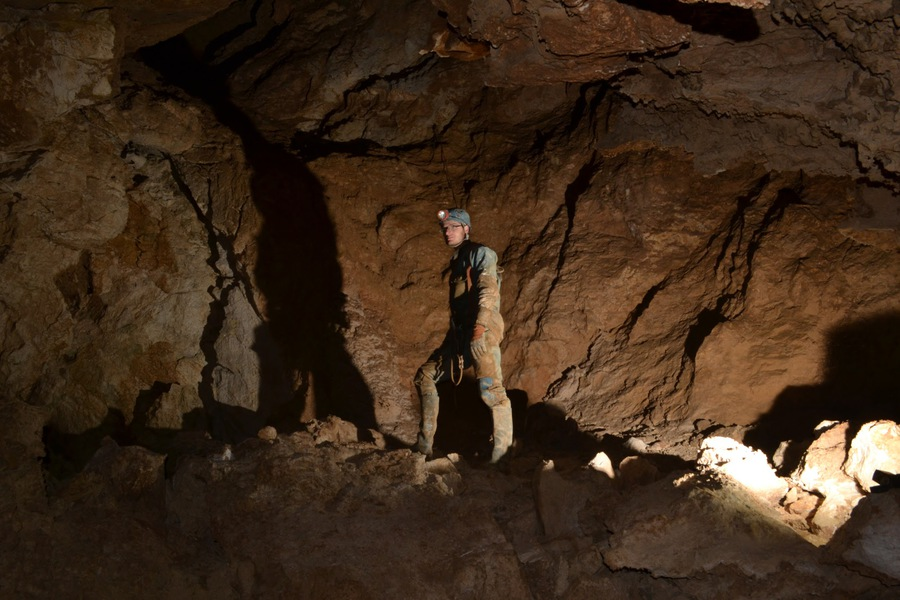
\includegraphics[width=\linewidth]{images/2013/tetley-sam-2013/rhys_hawaii.jpg}}
		\caption{}
		\label{hawaii}
	\end{subfigure}
	\vspace{5pt}
	\begin{subfigure}{\linewidth}
		\frame{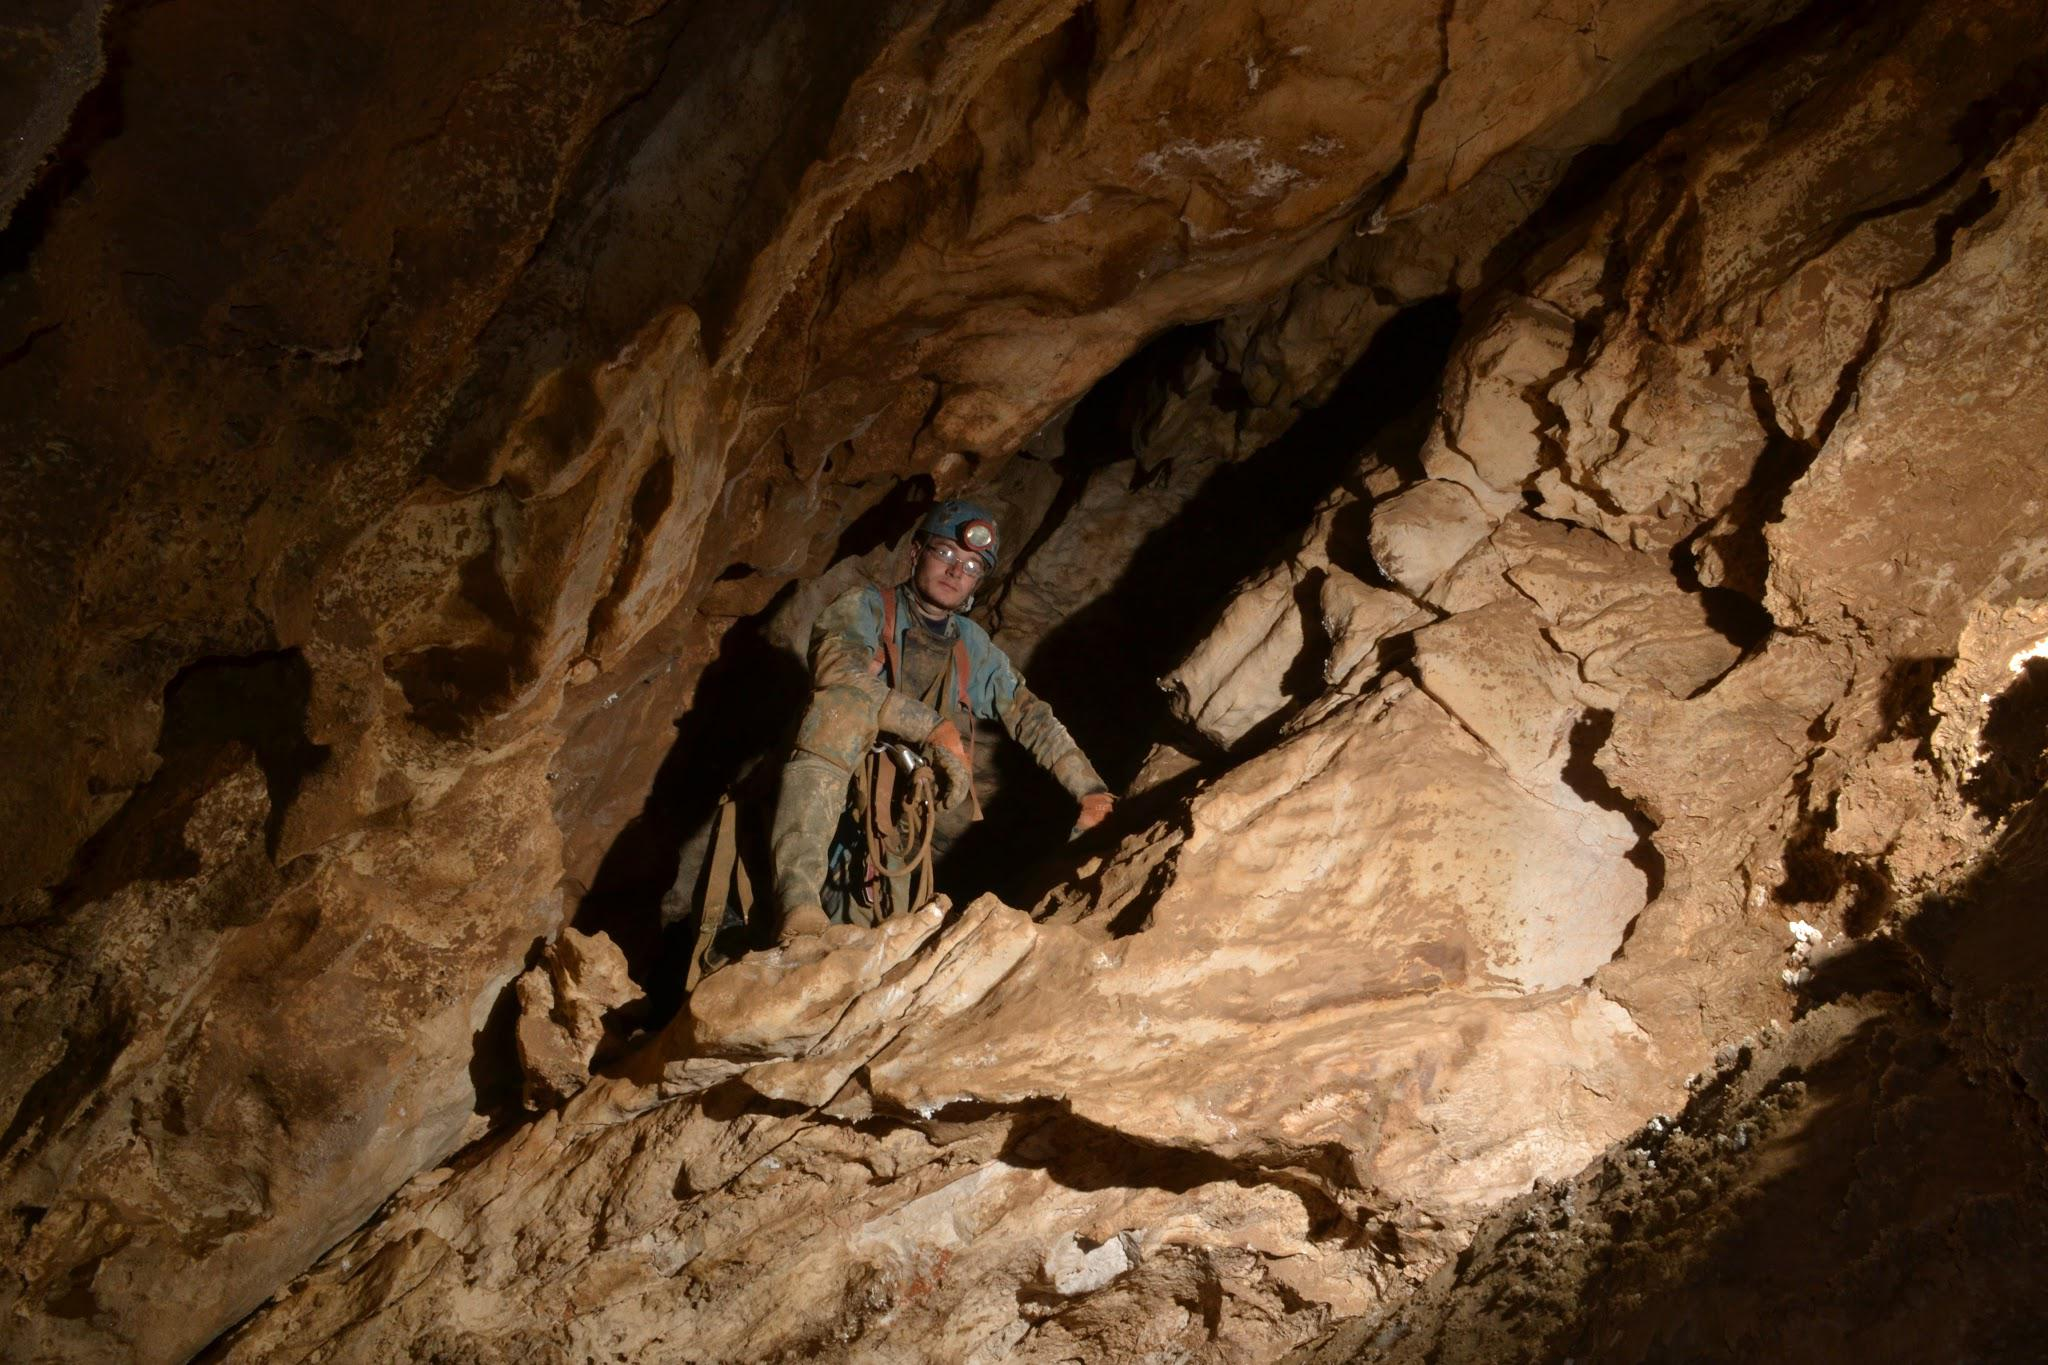
\includegraphics[width=\linewidth]{images/2013/tetley-sam-2013/rhys_lost_miles.jpg}}
		\caption{}
		\label{lostmiles}
	\end{subfigure}
	\caption{\emph{(a)} \protect\passage{Hawaii} junction, at the bottom of th extremely muddy \protect\passage{Stuck in Paradise} pitch \emph{(b)} \protect\passage{Lost Miles} passage --- Rhys Tyers}
	\label{}
\end{pagefigure}
  
	\begin{marginfigure}
\begin{tikzpicture}
\node [name-dest] (box){%
    \begin{minipage}{0.80\textwidth}
     \begin{itemize}
    \item Rhys Tyers
    \item Dave Kirkpatrik
    \item Christ Keeley
    \item Dave Wilson
    \item Pete Hambley
    \end{itemize}
    \end{minipage}

};
\node[fancytitle, right=10pt] at (box.north west) {Jailbreak};
\end{tikzpicture}
\end{marginfigure}

\section{Discovery of Jailbreak}
 
A group of us were meandering across the western edge of the plateau. Dewi and Dave had been poking in all the B series of the holes. I had my fair share of being inserted into exactly Rhys shaped holes, a couple of which went further than my body length.
 
It was sunny and we were happy to be in the open air. As we neared the cliff in an inconspicuous valley I spot a couple of small holes right next to each other. Peering in they immediately join up, the pillar in the centre forming a single bar, barring our entrance (ha). Beyond a dusty body sized tube invited us in. 

We each had a go with the hammer. Trying to chip at the solid rock bar. Chris Keeley steps up and from somewhere deep within unleashes the power of Thor. Thousands of hours of metal music and the power of long forgotten Norse mythology flowing through his long golden hair. He screams and attacks the rock, again and again and again. Within a few minutes its gone, all that’s left are two sharpish protrusions and a lot of rock flour littering the grassy bank. 
 
As the most sinous caver present (that had his caving kit) I am given the honour of inserting myself first. It’s a helmet off affair. Slither, slither, cough, cough, fuck thats dusty. I pop out into a swiss cheese chamber. Lots of little holes leading off. Most die very quickly. Through one, 30cm in diameter, there is daylight and Dewi gets a photo of me in there. One is very interesting though. Drawing a small draft I follow it and it drops, 90 degrees downwards. Gosh, a pitch. Could it go?
 
We return later. Me, DKP and Chris Keeley. I place a bolt or two, so does DKP. DKP descends first. The pitch, beautifully white and clean, we call \passage{Isengard}. I ask how it looks. 

\begin{figure*}[t!]
\checkoddpage \ifoddpage \forcerectofloat \else \forceversofloat \fi
\centering
\begin{subfigure}[t]{0.42\textwidth}
\centering
\frame{\includegraphics[width=\linewidth]{"images/2013/rhys-jailbreak-2013/pete-hambley-jailbreak__1_".jpg}}
 \caption{}\label{water chamber below helm's deep}
\end{subfigure}
    \hfill
    \begin{subfigure}[t]{0.56\textwidth}
        \centering
        \frame{\includegraphics[width=\linewidth]{"images/2013/rhys-jailbreak-2013/pete_jailbreak__1_".jpg}} 
        \caption{} \label{HelmsDeep}
    \end{subfigure}
    
    \vspace{0.3cm}
    \begin{subfigure}[t]{\textwidth}
    \centering
        \frame{\includegraphics[width=\linewidth]{"images/2013/rhys-jailbreak-2013/rhys-jailbreak__1_".jpg}} 
        \caption{} \label{Touching the Void}
    \end{subfigure}
    \caption{
    \emph{a} There were many Rhys-sized tubes on this part of the cliff face, most of which died within a metre or two.
    \emph{b} Rhys inserting himself through the entrance squeeze
    \emph{c} At the bottom of Isengard pitch in the Barrows}
\end{figure*}

“Ummmmm............you should come down here”
 
Are there sweeter words to hear when caving? That divulgence that there is something indescribable or something better left to your own eyes to see. I bomb down the pitch and scramble up the bouldery passage at the bottom to join DKP. He is standing on the edge, where the passage intersects  a large chamber. Nice! Chris Keeley joins us and we excitedly bumble down into the chamber.
 
There are a series of chambers in fact, joined by low sections. To the South they head upwards and veer towards to the cliff face. The floor get closer to the ceiling. There are a couple of 2m deep holes in the floor, nearly the size of the chamber, leaving just a ledge around the edge to climb around on. At the end the floor reaches near the ceiling and further passage is choked with choss. Through a crack in the wall you can perhaps see a smidgen of daylight.
 
We climbed down into a couple of the holes, most have nothing of interest in. One has a narrow bedding plane that you can crawl further into. We would spend a little while on a subsequent trip trying to dig this without much success. 
 
Heading North from where we originally dropped in, a low pebbly crawl brings you into another large chamber. The floor is rocks and boulders and they dip towards the centre, maybe a dig? At the far end a drip has carved a narrow tube downwards next to the wall. We have a poke at it. And its got a few rocks blocking the way. \sidenote{On a subsequent trip we set up a rather elaborate (read basic) hauling  system and move a huge rock out of there. Down 6m or so a floor is reached and an impossibly tight bedding plane heads off.}
 
We name our find \passage{The Barrows} due to it’s dead nature. Who knows? There might be more but it’s so close to the cliff that any small ways on seem to have been shattered and filled with choss.

\name{Rhys Tyers}
	
\section{Bivi Musings}


\begin{verse}
\begin{centering}
Bingo Granny Song

CHORUS:

Be do, be do, be do, be do, \\
Be do, be do, be do, be do, \\
Be do, be do, be do, be do, \\
Bingo Granny Song!

Bingo    Granny,   she   had     a    pet    bunny  \\
Bingo    Granny,   she   didn't have   much    money,   but \\
Bingo    Granny,   she   didn't  really     care,       she could \\
Always go to  Bingo! 

\emph{(Chorus)}

Bingo    Granny,     in      the Bingo      Hall, \\
Dressed up smart, like   she  thinks   its    a      Ball, \\
Bingo    Granny,    got    to    get        that  big   win, \\
A  packet of fags,  and   a     bottle of gin!


\emph{(Chorus)}

Bingo Granny took the bunny one day, \\
To see if he had what it took to play, but \\
Bingo Granny, she wasn't too wise, the \\
Bunny ran off to become the big prize!

\emph{(Chorus)}

Bingo Granny, she searched everywhere, \\
She couldn't find him, not even a hair but \\
When she went out he was there at the door, \\
in a top hat a cigar in his paw

\emph{(Chorus)}

Now Harry the bunny he was such a star, \\
People came to see him from near and a-far \\
Bingo Granny she was no longer poor, \\
So she could go to Bingo much more.

\emph{(Chorus)}

\end{centering}
\end{verse}

\fullwidthbox{A storm hits the mountain}{After threatening to rain all morning, when the wind and rain finally came, it left destruction in its wake, ripping through the bivi and knocking down tents. I risked a visit to the pit and having trouble enough lighting the paper when the great rain hit. I briefly tried crawling under the corrugated iron, but it was grim and wet so I desperately scrambled back to the \protect\passage{Casino}, getting drenched in the process. 

I subsequently danced in my pants to an album of Kate Nash, really outdoing my gayness. At times, it felt as if the tent would take off, but it didn't. At some point, an extra tent appeared in our porch. To happily spend an hour or two in your tent, I recommend trying to tune in to Radio Kiss Kiss, FM something. Eventually, the rain ceased and I quickly returned to the bivi, where Kate, Dave and Saber were merrily making music. If the weather is ok, I thought I might go to \protect\passage{Tolmin} soon: it hit me strongly when Tetley told me I looked rough.
\protect\name{Sam Page}
}




	\section{Exploration of Area S}

\margininbox{Area S}{
     \begin{itemize}
    \item Gergely Ambrus
    \end{itemize}}{\explo}


\recipecorner{Prawn crackers}{
Useful if expecting people later.
\begin{citemize}
\item Wait until oil is hot and just spitting (test with a prawn cracker).
\item Add about 6 prawn crackers or 1 poppadum to the cage and gently lower into the fat. 
\item The cracker should expand instantly. 
\item  Once expanded, lift cage and empty crackers onto plate or Tupperware/unused bin bag or eating later. 
\end{citemize}
 }

\paragraph{$7^{th}$ August 2013: } Yesterday we went to check the draughting holes in \passage[valley]{Vrtnarija} valley that Dave was talking about. We followed the path that Janet and Antonio made. There are three interesting spots we found.

The first one is a vertical fault line, it opens up to a pitch that you wouldn't need a rope to go in. It is about 70\,cm wide and about 6\,m high, and then probably drops probably 20\,m. There is no draught that I could spot.
This one is \passage{S5}. Coordinates:

\begin{itemize}
	\item N 46.25254 , E 13.77087,Altitude: 1627\,m
\end{itemize}


Continuing along the path, ~150\,m before reaching the upper \passage[alp]{Razor}-\passage[alp]{Kal} path, on the right side, ~6\,m from the path, a strongly draughting boulder choke is found. The draught is about the same as \passage{S1}; it does need work but it is quite promising! The best looking lead in the area.
This one is \passage{S6}. Coordinates:

\begin{itemize}
	\item N 46.25053, E 13.77094, Altitude: 1570\,m
\end{itemize}

Further along the path, just ~50\,m from \passage{S6}, cold air is draughting from between the boulders. This is not really an entrance but it may be dug into something. This one is \passage{S7}. Coordinates:

\begin{itemize}
	\item N 46.25037, E 13.77139,  Altitude: 1560\,m
\end{itemize}

The area may be interesting for looking for further leads; there is definitely a good amount of air coming out.

\name{Gergely Ambrus}

\begin{pagefigure}
      \checkoddpage \ifoddpage \forcerectofloat \else \forceversofloat \fi
      \centering
              \frame{\includegraphics[width=\linewidth]{"images/2013/gergely-2013/tim-child-stitch".jpg}} 
       \label{Panorama}
  \caption{ A  panorama of the glacial cirque which makes up the head of \passage{Gardeners' World} valley, the whale bone and the main valley between \passage[mountain]{Tolminski Migovec} and \passage[mountain]{Vrh Nad \v{S}krbino} \pic{Tim Child}}
\end{pagefigure}

	\begin{marginfigure}
\begin{tikzpicture}
\node [name-dest] (box){%
    \begin{minipage}{0.80\textwidth}
     \begin{itemize}
    \item Rhys Tyers
    \item David Kirkpatrick
    \end{itemize}
    \end{minipage}

};
\node[fancytitle, right=10pt] at (box.north west) {Xanadon't};
\end{tikzpicture}
\end{marginfigure}

\section{The mighty Xanadon't traverse}
 
We'd just woken up. The fairy lights strung across the wall cast a dim white glow across our camp. Packets of Smash, noodles and a bewildering variety of soup lay scattered across the floor, daring us to combine them into  a homogeneous breakfast goop.The little stove, surrounded by half used and identical plastics bags of sugar and dried milk, was already roaring, producing the first of many pans of tea. We sat huddled in sleeping bags and fleece pajamas listening to hit songs of the eighties echo off the rock around us.


\begin{marginfigure}
\frame{\includegraphics[width=\linewidth]{"images/2013/rhys-xanadont-2013/camp-X-Ray_in_full_swing".png}}
\label{}
\caption{Camp \protect\passage{X-Ray} in full swing --- Iztok Mozir}
\end{marginfigure}
It's comfortable in camp, despite being 500 metres below the surface, and leaving is always hard. Dave and I had a plan though. A plan that would surely bring us glory and riches. So we shed our warm fleece and retrieved our damp wetsocks, furries and oversuits from the optimistic washing line that runs across the chamber. The damp, near freezing air that breezes through is not interested in drying our gear but we hang it up all the same, hoping that by some osmotic miracle we wake to dry clothes. Suited up, with a bag full of metal, rope and an overclocked Ikea drill we set off.

\margininbox{The plan}{

`After much faffing and two dinners we are finally getting ready for bed. Dave and I had a 6 hour ``push'' in which we found a bypass to the \protect\passage{Euphrates} super grim crawl that pops out in \protect\passage[Big Rock Candy Mountain]{Big Rock}. Tomorrow we intend to construct the \protect\passage{Xanadon't} traverse to access it. I will be drilling and Dave will presumably be complaining.'
\protect\mininame{Rhys Tyers}

`I dreamt about rocks.'
\protect\mininame{David Kirkpatrick}
}

The day before Dave and I had been in a promising bit of cave named \passage{Cuckoo's Nest}, a tall, dry and winding phreatic passage. We hadn't found the way to the main pushing front and had instead spent some time poking around every moderately human sized hole that the previous team may have missed. Towards the end of our trip, with no significant new passage to our name, I climbed up into a sandy chamber and followed a low crawl. My helmet scraped along the ceiling as I dragged myself past the final constriction to be greeted by nothing. The crawl flanged out into vast, inky blackness. I could barely contain my excitement, the prospect of a big new pitch all to myself was too much. I leaned tentatively out into the darkness and examined my new discovery. 

\begin{marginsurvey}
\checkoddpage \ifoddpage \forcerectofloat \else \forceversofloat \fi
\centering
 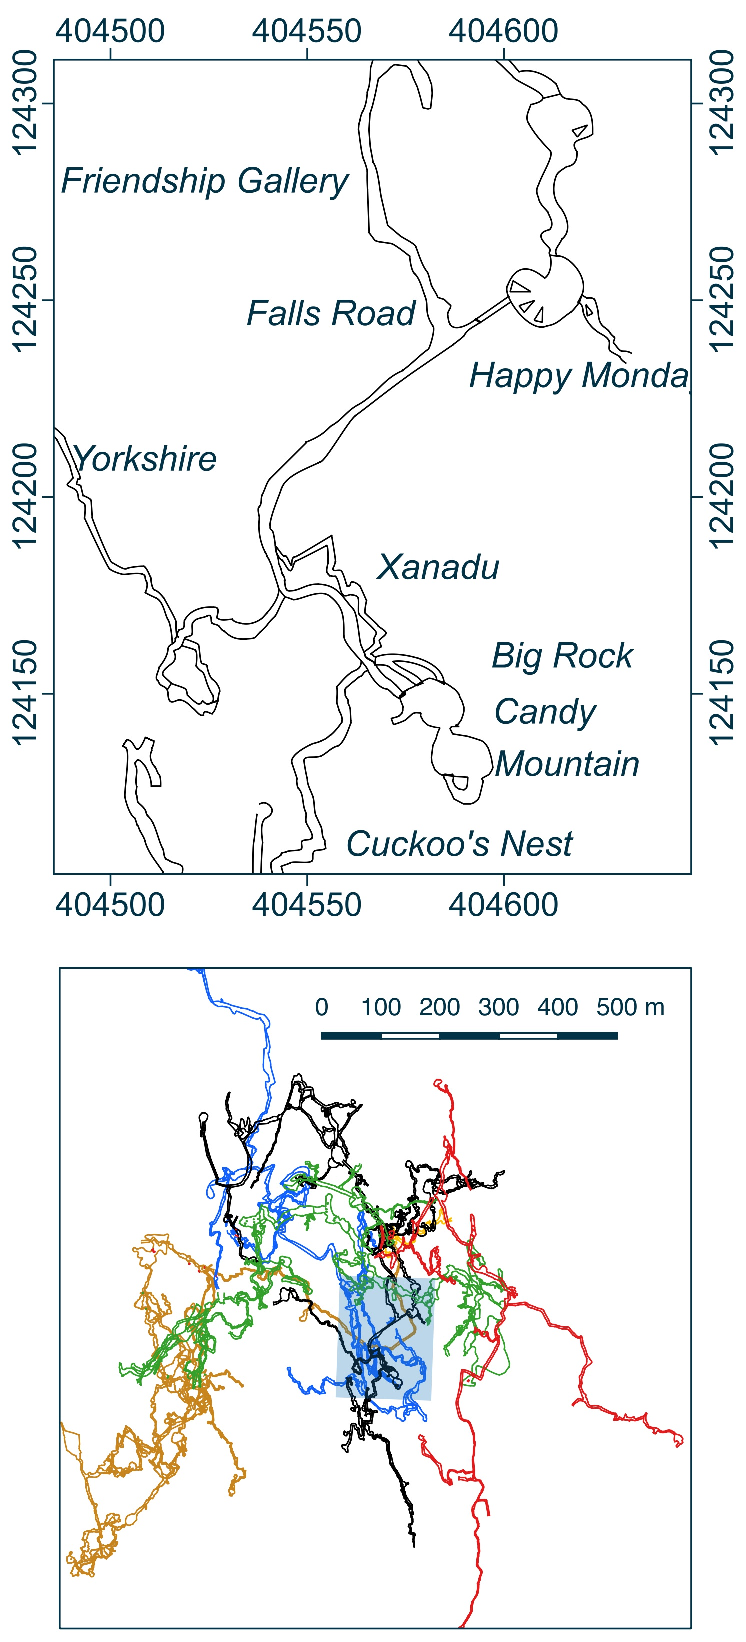
\includegraphics[width=\linewidth]{images/little_insets/bigrock_high_inset.pdf}
 \caption[Above Big Rock Candy Mountain]{Plan view of the \protect\passage{Big Rock Candy Mountain} area, including the \protect\passage{Xanadon't} Traverse, Slovenian National Grid ESPG 3794}
 \label{Red Cow inset}
\end{marginsurvey}


The bottom was lost in the depths and the far wall was only just visible. I turned to my left, and my heart sank. A rope. The thin white record of previous cavers dangled down, mocking. I recognized it fairly quickly, the only nearby large pitch was \passage{Big Rock Candy Mountain}, this must be a window into it. I scrambled back to Dave to tell him of my finding. Despite the let down this was still good news. The previous route to \passage{Cuckoo's Nest} was an awkward rift traverse followed by the most unpleasant muddy, wet, draughty crawl known to man. If we could rig a bypass down to the window I had found the new route would be an easy walk from camp, saving much time and psychological trauma for future explorers.

\begin{pagefigure}
\frame{\includegraphics[width=\linewidth]{"images/2013/rhys-xanadont-2013/rhys_hard_work".jpg}}
\label{}
\caption{Rhys hard at work --- Kate Smith}
\end{pagefigure}

So here we were, to rig the bypass. At the top of \passage{Big Rock Candy Mountain}, Dave and I set up a forward base. We had brought a gas stove, tea and as much marzipan and ginger cake as we could cram into a tackle sack. As the competent and confident caver of two years caving experience I was going to go down first. 

My plan was to rig a traverse from a rebelay I saw from the window. I grabbed a bag of rope and slung the drill strap around my shoulders and descended. The pitch wall is mostly an interesting combination of mud and flakes, neither of which are ideal for a bolt. After some swinging though I found a clean, solid looking face to bolt. I lined up the drill and pulled the trigger. The high pitched whine and dusty spray flying from the drill were satisfying and soon the drill bit was smoothly disappearing into the rock. The drill slowed, the whine turned to a grind and finally it sputtered a few angry clicks at me and stopped. 




I tried again, and again, and again. But the same each time, whine, grind, click, stop. Each time stopping faster until the drill would no longer spin. The battery must be dead, I thought, and climbed back up to Dave. A minor inconvenience at the most we thought and returned to camp to retrieve the spare battery. A while later I was back, inserting the drill into my half finished hole, a new block of chemical energy clenched between my thighs. But again the drill refused to cooperate. Whine, grind, click, stop. 

The drill must be fucked, I thought and climbed back up to Dave. A second inconvenience but we were not going to be deterred by shoddy Swedish engineering and again trudged back to camp to retrieve the hand bolting kit. 

\begin{pagefigure}
\centering
\begin{subfigure}[t]{0.49\textwidth}
\frame{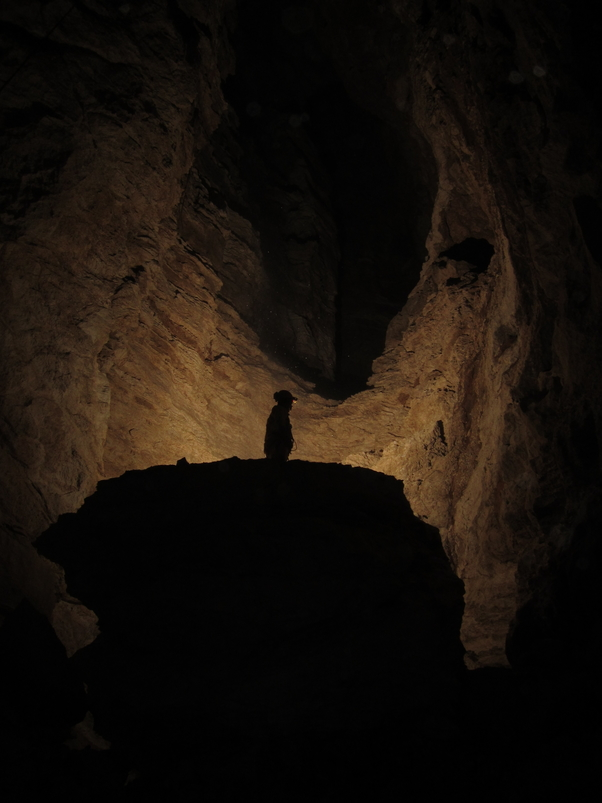
\includegraphics[width=\linewidth]{images/2013/rhys-xanadont-2013/bottom_big_rock_1.jpg}}
\caption{}
\end{subfigure}
\hspace{2pt}
\begin{subfigure}[t]{0.49\textwidth}
\frame{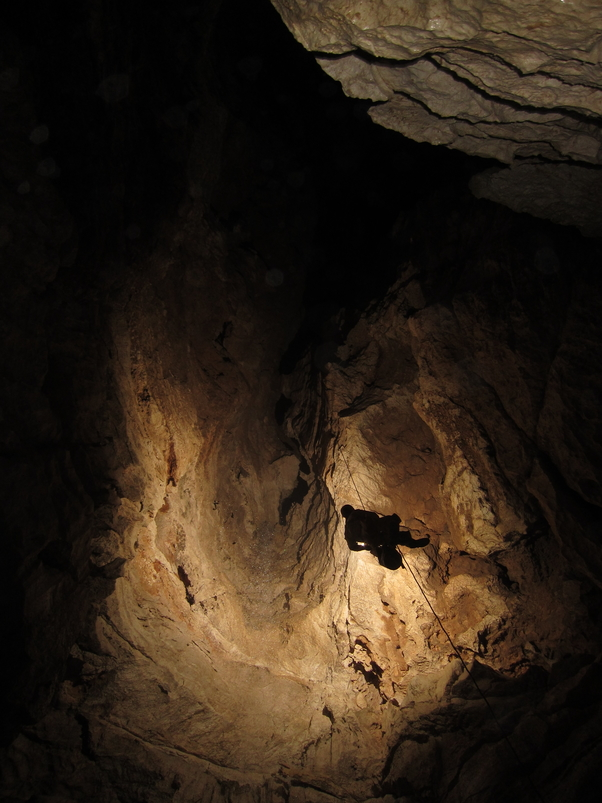
\includegraphics[width=\linewidth]{images/2013/rhys-xanadont-2013/bottom_big_rock_2.jpg}}
\caption{}
\end{subfigure}
\caption{\protect\passage{Big Rock Candy Mountain} ( named after the massive boulder in \textbf{(a)}) is a twin pitch located at the end of \protect\passage{Friendship Gallery}, over which it is now possible to traverse to reach the \protect\passage{Cuckoo's Nest} extensions --- Jarvist Frost}
\label{none}
\end{pagefigure}

Back at the now familiar spot, the half drilled hole staring at me, I wielded hammer and driver and got to work. I might whine, the driver might grind, the hammer might click but we would not stop. 

Tap, tap, tap. Tap, tap, tap. Tap, tap, tap. The clinking of the hammer against the driver calmed me into the familiar bolting rhythm. 

Tap, tap, tap. Tap, tap, tap. Almost done. 

Tap, tap, tap. Tap, tap, tap. Tap, tap, crack. 

Tap, tap, crack? 

I looked at my almost complete bolt. A crack had emerged from it and ran a few millimetres into the rock. Bollocks. I started again. But like my attempts with the drill, the second time was no better. Another crack halfway through bolting. Defeated, I climbed back up. We would need to regroup.

As I reached the top of the pitch something caught my eye. A row of bolts running across the top of the pitch. They would get us more than half the horizontal distance we needed! A miracle I thought as I got off the pitch. In front of me was a glowing silvery spirit, shaking and muttering about thrones and glory. Was this the deity that had placed the bolts? 

No, no, squinting my eyes revealed Dave's face under layers of silver survival blanket, clutching a pathetic tea light for warmth. `I have built a throne' he declared, through chattering teeth. And scuttered further back into the passage. I followed and Dave lead to a large pile of rocks. It's similarity to a throne stopped at `not being the floor' but Dave sat atop it proud as any regent had ever been. I decided it was probably Dave's turn to do some rigging and sent him to rig the mysterious bolts. I sat, drank some tea, ate some ginger cake and prepared for a long wait. I hoped I would be spared the madness that had overcome Dave.



Some time later I heard footsteps approaching. Was someone here to take my throne? My kingdom with its silver sky and single flame! The sky moved and Dave's face loomed over me.  `I rigged it' he says as my cognisance returned. I shivered my way out of the remaining foil and handed the tea light to Dave. Without the heat of the tea light or recent movement I made my way to Dave's new traverse, eager to get to the end and bolt the cold away. I vibrated along it, still none the wiser as to its creator. 

We would later find out that someone else also tried to reach a window in \passage[|see{Big Rock Candy Mountain}]{Big Rock} (a different one) but had failed, leaving these bolts behind. Their effort would not be in vain. From the end of the traverse I reckoned I was just two or three bolts away from reaching the window and emboldened by this thought I began once more. The rock here proved strong enough to hold my bolts and I at last I could see the window. I swung over and clipping my cowstail to a flake to hold myself in place, I started the final bolt. This final hang needed to be right over the window so that I could swing in, but to reach the ideal bolt position I had to lean out sideways and stretch out with the hammer. \bignote{Soon my arms were quivering with the exertion and I had to rest}. I was tired and the bolt was barely started. I hung for a while. So close yet so far. As my faith wavered and I considered turning back.

But then Dave called out. He was behind me. He had descended the original pitch and was now visible, on the other side. Stirred by companionship I bolted once more. It was slow going. Several times I shouted that I wanted to give up but Dave's friendly words reverberated around me. Sometimes he offered encouragement, mostly he complained about the position of his genitals within his harness. 

With a final tap I decided the bolt was secure and lowered myself into the window. Dave came across to examine the new route, finding me collapsed in the sand. Our quest complete, and eager to claim the praise and applause we would surely received, we returned to camp.

\name{Rhys Tyers}

	\section{Mig colloquialisms}

The following is a necessary update on the Migovec vernacular first published in the Hollow Mountain \citep{hm1}. This particular dialect of caving linguo is alive and thriving. 



\begin{description}
\item[Cow] Dried milk powder.
\item [Clag] What clouds look from the inside when enveloping the moutain
\item [Comf] Soft comfortable material to sit or lie on e.g. squares of chopped karrimats
\item [McGowan] A  dwarf pine based sofa so called because it resembles a bodybag containing the eponymous caver
\item [Faff]  To laze, waste time or take part in pointless labour
\item [Ey-Ohh] All purpose non-descript salutation
\item [Twatty] Adjective used to describe sections of cave which are tight, annoying or unnecessarily awkward.
\item [Schonky] Blanket adjective to describe anything dodgy, dangerous or loose, especially in caves
\item [Vitaminski] Powdered vitamin  sugary fizzy drink (comes in blue, yellow, orange and green flavours).

\begin{description}
	\item [slushies] Vitaminski mixed with ice from M10 on a hot day
\end{description}

\item [Blue Cloud] Patch of blue sky on a day of unrelenting clag
\item [Sunset] Evening ritual of fortified mountain tea consumption
\item [Slop] The evening cooked meal to go on the carbohydrates.
\item [the Hydro] A lovely swimming location near the Hydroelectric scheme of Tolminske Ravne
\item [$2^{nd}$ aid] Pills for hypochondriacs
\item [Old Lag] \textbf{O}wn kit, \textbf{L}eader, \textbf{D}river and experienced member of ICCC aged 25+
\item [Lightning Alley] A strip of fairly flat grass located high up on the Plateau. Not for the faint hearted.
\item [M10] Don't fall down M10
\item [Plateau] Undulating surface of Tolminski Migovec, anything between the Kuk and Mig trig points
\item [Mig] our spiritual home
\item [Union/La\v{s}ko polemic] Argument about the various merits of the two available beers in Slovenia. \sidenote{They are from the same manufacturer}

\end{description}


	\begin{marginfigure}
\begin{tikzpicture}
\node [name-dest] (box){%
    \begin{minipage}{0.80\textwidth}
     \begin{itemize}
    \item Rhys Tyers
    \item Clare Tan
    \end{itemize}
    \end{minipage}

};
\node[fancytitle, right=10pt] at (box.north west) {RCC Passage of the Year};
\end{tikzpicture}
\end{marginfigure}

\section{A Name Fit for the Lead}


\passage{Invictus} feels a long way from home. My pushing trip there with Tetley in 2012 were at the time the hardest thing I had physically done. I believe one of the trips I did was in excess of 22 hours. And now we were back to push further than the furthest there was. Clare and I, a crack team if ever there was one. 

Down the thick mud of \passage{Stuck in Paradise}, past the infested \passage{Hawaii} and into \passage{Penitence}. Half an hour or so of crawling on sharp pebbles. The sort that shatter as you place your weight on them. And then into the comparitive respite of \passage{Salvation}, where the floor is merely sand, but the ceiling no higher. Past the low junction, one side entirely full of sand. An easy dig were it 700m higher. Through the boulder choke that Tetley and I had cleared last year (and the one that had briefly entombed him). Onwards through the bizarre shattered chambers of \passage{Brave New World}, ignore the drippy inlet that almost certainly goes nowhere, squeeze past the ceiling slab collapse and pop out into \passage{Invictus}. Great piles of sand crowd the sides of the chamber.

At the end of the sandy passage we reached our goal, a pitch I had been forced to leave last year. Invictus intersects a shaft about halfway up. Maybe 15m to the bottom. A small stream falls down from the top. We place some bolts, chuck the rope down, promise to fix the rub point when the passage goes. We did not need to follow through on the promise. 

At the bottom, a typical flat, white, clean washed floor. The stream from above splattering and collecting gradually towards the far side of the chamber. There a passage leads off. We poked our heads in. A sump. Pretty and blue amongst the white rock, but its terminality spoiling its beauty. We searched for a while at the bottom, and up in Invictus for a way around but to no success. The aven is a potential lead, but the rock seemed chossy and loose. A difficult climb at best.

We named our lacklustre find \passage{RCC Passage of the Year} in honor of the lacklustre award we had recieved from the Union. We headed back out. 

Unquenched for exploration we elect to pop into \passage{Hash} on our way past. The tight, upwards spiralling, dry inlet off \passage{Minestrone} had been pushed by more people than it's nature deserved and had revealed the expected pittance of passage. Wiggling our way to the top, we found the small chamber in which Sam and Tetley had stopped. We push on, into more upwards tight crawl. After a short while we reach a dog leg in the passage that Clare did not want to attempt. Two things are known about Clare; she is small, and she is crazy. I suspect it would be deeply unwise for anyone larger or saner to attempt to push further. 

We surveyed out and climbed back towards X-Ray, arriving dissapointingly early. So early that we could not yet kick the sleepers out of bed. We are no inexperienced pair though, so we construct Camp Gamma Ray to ease our wait. A foil survival blanket thrown over a washing line forms a tent. A gas stove fills said tent with heat and carbon monoxide. So we pass the hazy hours till our designated slot in camp.

\name{Rhys Tyers}

\begin{figure*}[b!]
\begin{tikzpicture}
\node [name-dest] (box){%
    \begin{minipage}{0.95\textwidth}
    \begin{multicols}{2}
\paragraph{July 20$^{th}$} --- `Yesterday's trip to \passage{Minestrone} was a lot of fun. Looked at the little leads going off and Kate's climb. All became little squeezes with no draught. Except a climb (cairn at base of it) around PSS 21 and PSS 24, which leads to a downward sloping body sized tube which draughts. I went down it a good 5-10m but it seems to go on forever and felt too committing to do without help/rope. \passage{Hash} is a new lead found by Tim on the way back. Around 30-40m down Lost Miles from Hawaii is a climb up on the left hand side. PSS for \passage{Hash} is at start of climb. Left at draughting body sized crawl as we were short of time.' \name{Clare Tan}

\paragraph{July 22$^{nd}$} --- `Oh, also, we went and pushed \passage{Hash}, adding around 25 metres to what Tim \emph{et al.} had surveyed previously. Hash is fucking twatty and does continue beyond what we surveyed. Problem, only Tetley could fit through the squeezed just beyond our last survey leg. It was so close, just my shoulders are slightly too broad..with some tools we could've enlarged it but we would have had to gone back through to collect them. Beyond the squeeze, the passage continues upwards into a small chamber, 3m wide, 8m tall with a tight passage continuing off at the top. (all according to Tetley of course). Go push you narrow shouldered people.' \name{Sam Page}

\paragraph{August 1$^{st}$} ---`I am currently sat in a big silver bag in \passage{Friendship Gallery} with Clare. Today we pushed and killed \passage{Invictus}. It ends in a very tight rift with a puddle. The 20m of passage is named `\passage{RCC Passage of the Year}'. We also pushed \passage{Hash} to a tight chicane crawl thing that is is inadvisable for people bigger than Clare to go down. All in all got about 50m of passage. The silver bag, `Camp Gamma Ray' is very \sout{warm} grim.' \name{Rhys Tyers}
 \end{multicols}
    \end{minipage}

};
\node[fancytitle, right=10pt] at (box.north west) {The story of Hash --- the eventual death of a lead for the connoisseur};
\end{tikzpicture}
\end{figure*}
	\begin{marginfigure}
\begin{tikzpicture}
\node [name-dest] (box){%
    \begin{minipage}{0.80\textwidth}
     \begin{itemize}
    \item Rhys Tyers
    \item Oliver Myerscough
    \end{itemize}
    \end{minipage}

};
\node[fancytitle, right=10pt] at (box.north west) {Slinging in the Rain};
\end{tikzpicture}
\end{marginfigure}

\section{Leads in the Labyrinth}
 
Despite much planning and scheming over the course of the year Oli and I had conspicuously managed to avoid caving with each other for most of the expo. With just a few days to go before derig we finally decided to put our plans into action. On a night train of course.
 
Oli and I were quick and slick down the entrance series. We caught up with Chris Keeley and co just before camp. We overtook and geared up in the staging area in \passage{Friendship Gallery}. With an inappropriate feeling of optimism we packed the drill, gearing up for a big pitch series. Oli had spun wild tales of bottomless pitches and caverns measureless to man. Based on my previous experience of \passage{Yorkshire} and it’s continuations, I was doubtful. I found it hard to believe that the tight, thrutchy rift would develop into anything other than tight thrutchy rift but perhaps it would break into the master system and the mystery of \passage{Mig} would solved. 


 \begin{marginfigure}
\centering
\frame{\includegraphics[width=\linewidth]{"images/2013/rhys-sling-2013/rhys-skrbina".jpg}}
\label{Rhys Skrbina}
\caption{Rhys Tyers stands at the summit of \protect\passage{Vhr Nad Skrbino} --- Dave Kirkpatrick}
\end{marginfigure}

 
We snuck past the sleeping cavers in camp. Our gear clanked loudly and our swearing echoed as we climbed over the awkward mud wall beyond camp. Following \passage{Friendship Gallery} to the end, past the \passage[|see{Big Rock Candy Mountain}]{Big Rock} turning, brings you to a boulder strewn chamber. Somewhere here is a dug route downwards. It’s long and sinuous and impresses upon you the lack of fear the Jana and co (the diggers) had. A couple of small chambers, and a big drippy pitch bring you to an immature streamway. Do not follow the water, climb above the water chamber (Tetley and I had followed the water previously down far too much grim immature stream, still a lead though). 
 
Then it’s  just a matter of following the thrutchy vadose passage. Occasionally Oli led me into a dry meander that would then rejoin the streamway again. I don’t think anyone has followed the stream all the way down, so who know’s if there’s anything off there. At some point there’s an interesting climb down into the stream again where you cross over the rift and double back. There’s also a small section with a quite a few dry passages heading off, supposedly thoroughly explored by Saber and Oli. 
 
Once at the limit of exploration Oli coaxed me forwards, to the head of the ‘bottomless’ pitch. Gently I edged forwards until I could see down, all of perhaps 10 metres to the floor. Oli assures me that his previous claim was misremembering and not in fact a trick to lure me to his pet shit lead. Still, though not deep, the passage bellowed out into a middling sized chamber. With a big bag full of equipment we barely knew how to use there was nothing to stop us. Oli retrieved the drill, clipped in the drill bit, attached the battery and set to work tunneling a new home for our shiny raul bolts. 
 
Quite a while later, with no progress, and after several attempts at drilling in various spots  Oli me what he thought the problem could be. Super hard rock? A blunt drill bit? Maybe he wasn’t pushing the drill hard enough. I pondered. 

`You've got the drill in reverse' I offer. 

We swap places and with the drill rotating in the correct direction I try again. I successfully drill a hole and place a bolt but carelessly hammer it on so that the end deforms and I can’t get the nut on. So much for that. Frustrated and itching to get down the pitch we scanned the surrounding rock. We located a nodule of rock sufficiently large to abseil off (but not too large as to make you overconfident in its abilities as an anchor, that too would be a mistake) and a second, further back in the passage. We gave each a fetching green nylon choker, attached our ropes and I headed down.
 
Unfortunately our carefully chosen anchors placed me perfectly under the small stream that we’d been following all the way from \passage{Yorkshire}. I scrambled desperately at the wall and clawed my way out of the water. I looked around. I wanted a nodule, flake, a stal, anything for a deviation. Smooth walls offered me nothing but glistening reflections. I was however gripping a small crack in the wall. I tied an overhand in both ends of a sling, rethreaded one (for a krab) and inserted the other end of the sling into the crack and pulled it, till the single overhand was wedged. I clipped the krab above me and carefully loaded my crack deviation. It held.

\begin{marginfigure}
\centering
\frame{\includegraphics[width=\linewidth]{"images/2013/rhys-sling-2013/izi-monatip".jpg}}
\label{Monatip-rigging}
\caption{Rigging one of the new finds in Monatip--- Iztok Mozir}
\end{marginfigure}

At the bottom it became apparent that we were just on a ledge. The ledge was flat and washed clean. A 5m by 5m by 15m deep hole was in front of us, large boulders perched precariously above it.  Across the holes, at the same height as the ledge was a crawl going off. To the right was a crack, filled with boulders, descending into the shaft. Up from the crack a small hole led off. A crawl can be seen heading off but looks a little immature. We headed back and began thinking about how to get down the pitch.
Oli decided it would be incredibly dangerous to attempt to descend the pitch without proper gardening first. I suspect he just wanted to push big boulders down the pitch. He pushed a couple, varying from the classic TV sized boulder to some approaching human size. They went down with a spectacular bang. He was right though, it didn’t take much to push them down. He went for another one. I winced expecting the loud crash but nothing came. The two Oli sized boulder had become wedged on the edge of the lip and the far wall (there was a sort of corner with the crack). On the near side it was stuck on a tiny protrusion from the wall. I tried to hit it with a hammer but it was surprisingly solid. We looked at each other. There was no way we could descend with this death hanging above us. 
 
Oli decided to solve this problem as he solves all his problems. He started throwing rocks at the rock. Gradually the rock inched further downwards. Each thrown rock budging it down another few millimetres. Eventually it fell. It was a close thing to as we were running out of rocks to `garden’ with.
 
We looked about for some good rock to bolt in but found none. Eventually we squeezed into the crack and found some suitable naturals to descend on. At the bottom we landed on what had been a clean flat floor, now littered with the remains of our gardening. The water trickled ahead into stooping passage and very quickly sumped. It was very pretty, all blue green against nice white rock but it wasn’t what we were hoping for. We climbed back up.
 
Going up the crack there was a small passage. We crawled up this a way until it brought us out in a small chamber with some water trickling from 5 or so metres above us. It might be possible to free climb this but you’d probably want to bolt it. Back down again and we turned our eyes to the final lead, the crawl across the other side of the chamber.
 
We edged our way round placing bolts wherever the rock had the fewest fractures. We were hand bolting by this point having become frustrated with our ineptitude with the drill. 3 or 4 bolts brought us safely into the crawl. Down the sandy abandoned phreatic passage, we came to a point where two boulders blocked the way. We tried moving them but they wouldn’t budge. 

\margininbox{Lead advice}{Beyond, the crawl continues, likely bypassing the perched sump. A bit of capping or even feather and wedging would get you past. \protect\mininame{Rhys Tyers}}
 
Back at camp we collapsed. I awoke 12 hours later and tried to cajole Oli into going pushing or maybe even heading out but he was not a man who could be moved. Another 10 hours passed.  We were alone, on the last pushing trip of the expo. We got up att 11pm or so, packed up as much as we could to get the f out of there. The next day everyone else would come down to haul the rest of the camp stuff out and the derigger would do the needful. The weather forecast predicted armageddon at 12am. As we packed we realised we could get everything into 5 bags, most of which would be relatively light. So we took 5 bags. Oli took the two heavy ones and I took the three light ones. Another 5 hours and we emerged into the morning light and drizzle. A few bleary faces greet us at the bivi.

\name{Rhys Tyers}

	\section{Discoveries big and small in the Hollow mountain}

\begin{marginfigure}
\begin{tikzpicture}
\node [name-dest] (box){%
    \begin{minipage}{0.80\textwidth}
     \begin{itemize}
    \item Clare Tan
    \item Iztok Mozir
    \end{itemize}
    \end{minipage}

};
\node[fancytitle, right=10pt] at (box.north west) {Atlantis};
\end{tikzpicture}
\end{marginfigure}

\section{ At the end Atlantis}
Pushed \passage{Brezno Slapov} with Izi last night, it was a great trip. Dropped a couple of pitches to get to a canyon/rift with a stream, followed it and eventually got to a sump. But taking a left turn down and inlet leads to the base of another wet pitch and a continuation of passage, but is was wet and we didn’t go on.
\name{Clare Tan}

\begin{marginfigure}
\centering
\frame{\includegraphics[width=\linewidth]{"images/2013/other-finds-2013/oli-fire".jpg}}
\label{Olifire}
\caption{On the last night on top of the mountain, all perishable food is ritually burned as Oliver Myerscough demonstrates with flour--- Kate Smith}
\end{marginfigure}

\section{Below Balamory}
\subsection{06/08/2013}
Exciting night of pushing yesterday. \passage{Clapton} pitch is a massive space. Effectively like two shafts right next to each other. We drop the shorter one. Couple of leads at the bottom. One has a bedding plane squeeze that stopped Maffi, it follows water to a small pitch, might join up with something off the other half of \passage{Clapton}.
We mainly pushed the other lead, schematic on facing page. It’s still open and going.Unfortunatley when we started to survey we discovered a crack in the clino glass. Which is why the tentative passage name is now \passage{Crack Shack} [ed. not on page reads “Renamed \passage{Pick Your Poison}]. There’s also alot of black sandy silt deposition in our passage, plus its in keeping with the cocaine theme...
Going back today to survey waiting for day trainers to arrive, listening to music, writing this t put off pissing....I really like caving and camping underground...
P.S. none of the leads were killed during this push!!!!

\name{Clare Tan}

\subsection{07/08/2013}
Went back to \passage{Clapton} yesterday to survey what we found the previous trip ~200m added to this years total. There are so many leads there we called it \passage{Pick Your Poison}. Will be dreaming about it now for the next 11 months...
I guess this is now my last few hours in camp. It’s been a great expo of caving for me - many thanks to all my pushing/camping partners: Saber, Izi, Rhys and Maffi for the excellent trips and company. Thanks also to all who have camped at \passage{X-Ray} for the laughs and great conversation.
Almost can;t believe another expo is drawing to a close...caving-wise I feel thoroughly satiated, but I’ve enjoyed myself so much that I don’t want it to end. Ah well, there’s always next year, and the year after, and the year after....I wonder if I’ll still be here in 10 years?
I should really go to sleep but my body doesn’t want to cooperate....Maybe it’s time to read Tet’s 15 page epic (from earlier in the expo.

\name{Clare Tan}

Still no inspiration, I guess Clare Tan has drained out of me even this, nor only all energy, while trying to figure out how to squeeze through thos passages we’ve found. Anyway it is the last day in \passage{X-Ray} this year. Wish this refuge was open the whole year. Aja! I want to thank Dave Wilson for the hint on \passage{Balamory}. He made possible the biggest discovery this year! And with this he also gave Erik and me the sensation of pioneers. Thanks Dave! (well this sensation we get every time we push something nice but this one could be compared with findings of Columbus, Marco Polo, Juri Gagarin :) ) Thank you Erik, thank you Clare Tan. Thank you everyone that made Mig adventures possible. Over an out.
\name{Grega Maffi}


\begin{figure*}[b!]
\begin{tikzpicture}
\node [name-dest] (box){%
    \begin{minipage}{0.95\textwidth}
    \begin{parcolumns}{2}
\paragraph{July 20$^{th}$} --- ‘Yesterday’s trip to \passage{Minestrone} was a lot of fun. Looked at the little leads going off and Kate’s climb. All became little squeezes with no draught. Except a climb (cairn at base of it) around PSS 21 and PSS 24, which leads to a downward sloping body sized tube which draughts. I went down it a good 5-10m but it seems to go on forever and felt too committing to do without help/rope. \passage{Hash} is a new lead found by Tim on the way back. Around 30-40m down Lost Miles from Hawaii is a climb up on the left hand side. PSS for \passage{Hash} is at start of climb. Left at draughting body sized crawl as we were short of time.' \name{Clare Tan}

\paragraph{July 22$^{nd}$} --- ‘Oh, also, we went and pushed \passage{Hash}, adding around 25 metres to what Tim et al had surveyed previously. Hash is fucking twatty and does continue beyond what we surveyed. Problem, only Tetley could fit through the squeezed just beyond our last survey leg. It was so close, just my shoulders are slightly too broad..with some tools we could’ve enlarged it but we would have had to gone back through to collect them. Beyond the squeeze, the passage continues upwards into a small chamber, 3m wide, 8m tall with a tight passage continuing off at the top. (all according to Tetley of course). Go push you narrow shouldered people.' \name{Sam Page}

\paragraph{August 1$^{st}$} ---‘I am currently sat in a big silver bag in \passage{Friendship Gallery} with Clare. Today we pushed and killed \passage{Invictus}. It ends in a very tight rift with a puddle. The 20m of passage is named '\passage{RCC Passage of the Year}'. We also pushed \passage{Hash} to a tight chicane crawl thing that is is inadvisable for people bigger than Clare to go down. All in all got about 50m of passage. The silver bag, “Camp Gamma Ray” is very \sout{warm} grim.' \name{Rhys Tyers}
 \end{parcolumns}
    \end{minipage}

};
\node[fancytitle, right=10pt] at (box.north west) {The story of Hash --- the eventual death of a lead for the connoisseur};
\end{tikzpicture}
\end{figure*}

\begin{pagefigure}
      \checkoddpage \ifoddpage \forcerectofloat \else \forceversofloat \fi
      \centering
    \begin{subfigure}[t]{\textwidth}
    \centering
        \frame{\includegraphics[width=\linewidth]{"images/2013/other-finds-2013/lethe_sifon_2".jpg}} 
        \caption{} \label{lethe sifon 2}
    \end{subfigure}
    
          \vspace{0.3cm}
          
    \begin{subfigure}[t]{0.555\textwidth}
        \centering
        \frame{\includegraphics[width=\linewidth]{"images/2013/other-finds-2013/clare_in_lethe".jpg}} 
        \caption{} \label{clare in lethe}
    \end{subfigure}
    \hfill
    \begin{subfigure}[t]{0.418\textwidth}
        \centering
        \frame{\includegraphics[width=\linewidth]{"images/2013/other-finds-2013/lethe_canyon".jpg}} 
        \caption{} \label{lethe canyon}
    \end{subfigure}

    \caption{
    \emph{a} The cascading steam from \protect\passage{Brezno Slapov} ends at an ominous sump (-802m)
    \emph{b} Clare Tan navigates through the stream and canyon passage below \protect\passage{Brezno Slapov}.
    \emph{c} Water from the stream passage accumulates in deep pools --- Iztok Mozir }
\end{pagefigure}

\begin{figure*}[h!]
      \checkoddpage \ifoddpage \forcerectofloat \else \forceversofloat \fi
      \centering
              \frame{\includegraphics[width=\linewidth]{"images/2013/other-finds-2013/kate-end-of-expo-2013".jpg}} 
       \label{end expo}
  \caption{ --- Tim Child }
\end{figure*}

\begin{figure*}
\begin{tikzpicture}
\node [table] (box){%
    \begin{minipage}{\linewidth}
    \centering
    \begin{tabular}{lrrrr}
    Sector & \multicolumn{1}{l}{Passage name} & Survey length (m) & Stations & Average leg (m) \\ \midrule
    \multirow{2}[0]{*}{Apollo} & \multicolumn{1}{l}{Apollo Traverse} & 21.63 & 5     & 5.41 \\
          & \multicolumn{1}{l}{Beetlejuice} & 55.46 & 9     & 6.93 \\ \midrule
    \multirow{5}[0]{*}{Balamory} & \multicolumn{1}{l}{Bingo Granny} & 21.06 & 5     & 5.27 \\
          & \multicolumn{1}{l}{Clapton} & 51.04 & 11    & 5.10 \\
          & \multicolumn{1}{l}{Kokain Lab} & 69.8  & 12    & 6.35 \\
          & \multicolumn{1}{l}{Kokain Rute} & 113.09 & 21    & 5.65 \\
          & \multicolumn{1}{l}{Pick Your Poison} & 191.66 & 28    & 7.10 \\ \midrule
    Kamikaze & \multicolumn{1}{l}{Rural Underground} & 101.29 & 23    & 4.60 \\ \midrule
    \multirow{4}[0]{*}{Lower Pleasures} & \multicolumn{1}{l}{Curiouser and Curiouser} & 69.42 & 15    & 4.96 \\
          & \multicolumn{1}{l}{Curiouser and Curiouser 2} & 35.45 & 14    & 2.73 \\
          & \multicolumn{1}{l}{Slinging in the Rain} & 86.01 & 17    & 5.38 \\
          & \multicolumn{1}{l}{Labyrinth} & 95.94 & 31    & 3.20 \\ \midrule
    \multirow{6}[0]{*}{Stuck in Paradise} & \multicolumn{1}{l}{Hash} & 39.64 & 14    & 3.05 \\
          & \multicolumn{1}{l}{Hash2} & 26.07 & 8     & 3.72 \\
          & \multicolumn{1}{l}{Hash3} & 21.4  & 9     & 2.68 \\
          & \multicolumn{1}{l}{Lethe} & 138.97 & 30    & 4.79 \\
          & \multicolumn{1}{l}{RCC passage of the year} & 26.5  & 7     & 4.42 \\
          & \multicolumn{1}{l}{We're not Alone} & 39.96 & 7     & 6.66 \\ \midrule
    \multirow{8}[0]{*}{Xanadu } & \multicolumn{1}{l}{500m} & 15.59 & 7     & 2.60 \\
          & \multicolumn{1}{l}{Cuckoo's Nest} & 220.73 & 41    & 5.52 \\
          & \multicolumn{1}{l}{Dwarf Pine} & 33.2  & 6     & 6.64 \\
          & \multicolumn{1}{l}{Hydrophobia} & 63.42 & 11    & 6.34 \\
          & \multicolumn{1}{l}{Rejuvenation Rift} & 103.39 & 29    & 3.69 \\
          & \multicolumn{1}{l}{Straightjacket} & 24.31 & 11    & 2.43 \\
          & \multicolumn{1}{l}{Time Bandits} & 126.56 & 22    & 6.03 \\
          & \multicolumn{1}{l}{Xanadon't} & 34.28 & 12    & 3.12 \\ \midrule
          &       &       &       &  \\
    \textbf{Total} &       & \textbf{1825.87} &       &  \\
    \end{tabular}%
  \label{tab:addlabel}%
  \end{minipage} };
\node[tabletitle, right=10pt] at (box.north west) {Number crunching};
\end{tikzpicture}
\end{figure*}


\begin{figure*}[t!]
\centering
\frame{\includegraphics[width=\textheight, angle=270]{"images/2013/other-finds-2013/2013plan".pdf}}
\caption{}
\label{plan 2013}
\end{figure*}

\begin{figure*}[t!]
\centering
\frame{\includegraphics[height=\textheight]{images/2013/other-finds-2013/ee2013.pdf}}
\caption{}
\label{EE 2013}
\end{figure*}
	\thispagestyle{endchapter}

\begin{tcolorbox}

\vspace{80pt}
	\lettrine{T}{h}{e} 2013 expedition drew to a close. The pushing had been harder, 
	and perhaps not as immediately rewarding as the previous year. The vast pitches and storming phreatic were 
	elusive in most areas. The one exception of course being the surprise find below \passage{Balamory}; the big
	active rift pitch series from \passage{Kokain} to \passage{Pick Your Poison}. But \passage{Minestrone} had 
	failed to yield to extensive pushing, \passage{Invictus} gave up with a terminal aven, \passage{Brezhno Slapov}
	proved too wet to push far. 
	
	Despite this 1.8km of passage was found, at great depth. After a final push to \passage{Slinging in the Rain} 
	Rhys Tyers and Oliver Myerscough put the cave to sleep for the year, hauling out the 5 bags they managed to 
	pack X-Ray into.
	
	The weather had been exceptionally good for the entire expedition and this was reflected in the general morale. 
	To take advantage of the good weather the expedition decamped the mountain a couple of days early to enjoy the 
	baking heat of Tolmin, and the cooling waters of the Soča river. The JSPDT and ICCC parted ways for the year.

	The longest cave in Slovenia would be waiting for them next year.

\end{tcolorbox} 
	\backgroundsetup{	scale=1,
					color=black,
					opacity=1,
					angle=0,
					contents={%
							  \includegraphics[height=\paperheight]{images/backgrounds/dave-2013.jpg}
 					}
	}
\BgThispage

 		\newpage
\begin{tcolorbox}
	


\chapter{2014 - Zkosi Zrcalo}
		\lettrine{I}{n} many ways the 2014 expedition adopted from the previous year's format. The duration of expedition was set at 5 weeks, between 11th of July and 14th August and in total 22 cavers made their pilgrimage to the hollow mountain, staying anywhere between 1 and 5 weeks. Camp \emph{X-Ray} in \emph{Friendship Gallery} as the chosen base for deep exploration. Most of the new passages visited this year were found south of \emph{Atlantis} and left as an expanding network of passages with many questions unanswered. The discovery of a large chamber and an active stream below made for a hydrological puzzle. 

		Hardy cavers were lured towards the deep end, where, after the discovery of the large series of rifts below Balamory, they headed down a winding stream passage until they met the water table at Aja! sump.  Due to the distance and hostility of the remaining 2013 pushing fronts, the feeling that some of the leads might be out of reach of the more novice cavers started had been circulating. In the end however, the discovery of 1.2km of cave, all of it at depths greater than 500m and sometimes as far as 3hrs from the camp, involved all the expedition's novices and dispelled any qualms about the accessibility of the pushing fronts.

 		The noteworthy visit to Colarado Sump a decade after its original discovery yielded, on top of its more obvious rerigging and rebolting by-products, an unexpected result: the previously 'terminal looking' sump revealed to be a mere duck. Jarvist Frost also put significant effort in laying the foundations for a deep, lightweight underground camp near \emph{Red Cow} with sights on \emph{Watership Down}, to this day the deepest point in the entire System.
		\\
		\\
		\\
		
\end{tcolorbox}
	\backgroundsetup{	scale=1,
					color=black,
					opacity=1,
					angle=0,
					contents={%
							  \includegraphics[height=\paperheight]{images/backgrounds/Rhys_Red_Cow.jpg}
 					 }
	}
\BgThispage
	
	\begin{marginfigure}
\begin{tikzpicture}
\node [name-dest] (box){%
    \begin{minipage}{0.80\textwidth}
     \begin{itemize}
    \item Rhys Tyers
    \item Clare Tan
    \end{itemize}
    \end{minipage}

};
\node[fancytitle, right=10pt] at (box.north west) {Bivi};
\end{tikzpicture}
\end{marginfigure}

\section{A rather cold welcome}

When Rhys Tyers and Clare Tan flew out a week before the main 2014 expedition, they had no inkling that the hollow mountain reserved a rather unpleasant welcome for them both, for after a long ascent through whirling milky white clouds and dense, cold and drippy dwarf pine they broke onto a bleak landscape. The sun had not started to pierce through the shifting cloud cover, giving the place a desolate, empty look. Less empty however was the bivi shakehole, which the wan light barely touched: a large snow plug occupied the space which was to be filled with the buzz and bustle of excitement only a score of like-minded explorers can produce.

This was rather problematic since it kept the bivi temperature far below that the plateau --- at the best of times, the bivi shakehole is a couple of degrees cooler than elsewhere --- prevented the access to the stone circle, rendered the usual washing space impracticable and finally because the melt runoff kept mixing with years of bivi sedimentation, the result of which was a most repugnant mixture. 

As the main core of the expedition arrived however, large numbers of helping hands, adequate job division and most of all, a determination to vanquish the uninvited iceberg saw a large operation of snow removal take place. Some was hauled out of the shakehole and dumped into M10 --- maybe a fraction resisted further melting and was later hauled up for drinking water the following year--- another portion sawed off and sculpted and one particularly large lump provided shelf space for the drying dishes and cutlery.

Little by little, the ice receded and the cold bivi nights turned more pleasant, even as news of further underground discoveries came floating back from the plateau. The weather improved gradually, and it was not without a pinch of sadness that we saw the last of it meekly retreating below the scree under a hot summer's afternoon. 

\name{Tanguy Racine}

\begin{pagefigure}
\checkoddpage \ifoddpage \forcerectofloat \else \forceversofloat \fi
   \centering

       \begin{subfigure}[t]{0.393\textwidth}
        \centering
        \frame{\includegraphics[width=\linewidth]{images/2014/welcome-2014/dsc_1239.jpg}}
        \caption{} \label{Snow plug}
    \end{subfigure}
    \hfill
     \begin{subfigure}[t]{0.59\textwidth}
        \centering
        \frame{\includegraphics[width=\linewidth]{images/2014/welcome-2014/dsc_1333.jpg}} 
        \caption{} \label{Snow sawing}
    \end{subfigure}
    
    \vspace{0cm}
    \centering
    \begin{subfigure}[t]{0.59\textwidth}
        \centering
        \frame{\includegraphics[width=\linewidth]{images/2014/welcome-2014/dsc_1324.jpg}} 
        \caption{} \label{Snow burning}
    \end{subfigure}
    \hfill
    \begin{subfigure}[t]{0.393\textwidth}
        \centering
        \frame{\includegraphics[width=\linewidth]{images/2014/welcome-2014/dsc_1327.jpg}}
        \caption{} \label{Snow carving}
    \end{subfigure}

    \vspace{0cm}
    \begin{subfigure}[t]{\textwidth}
    \centering
        \frame{\includegraphics[width=\linewidth]{images/2014/welcome-2014/dsc_1252.jpg}}
        \caption{} \label{Panorama from mule path}
    \end{subfigure}
    \caption{
    \emph{a} The snow plug at the back of the bivi
    \emph{b} Sarah, cutting away of block of snow to uncover a stone seat
    \emph{c} Will French burning away at the iceberg.
    \emph{d} Carving, sawing and hacking at the edges of the snow plug
    \emph{e} On the mule path looking back towards Tolmin and the Soa valley. --- Rhys Tyers}
\end{pagefigure}
	\section{The death of Jailbreak}
	\margininbox{Jailbreak}{
				     \begin{itemize}
					    \item Rhys Tyers
					    \item Dave Kirkpatrik
					    \item Tanguy Racine
				    \end{itemize}
}{\dig}
	First impressions last a very long time. I still cherish my first memories of the caving club. Among them I recall clearly my first tree training session, the expedition talk a week before, and most important of all the first pub night. Myself and several other freshers on our first year of university sat with the older members of the club. There was a laptop on one of the wooden tables outside the Union bar so we gathered round to look at the photos of newly discovered galleries and caves. Rhys and Oli described a cave they had hammered their way through: \passage{Jailbreak}.

	Ten months later, it was hard to believe I was finally going to see this relatively exciting finding. While Dave Kp and Rhys gathered their caving kits, I grabbed a pulley from the stash of metalwork that lay in the middle of the \passage{Bivi}. Not two days before, Rhys had shown me the way down \passage{Vrtnarija}'s main shaft series, to the top of \passage{Tesselator}, a good third of the elevation difference between the entrance and the underground camp.
		\begin{pagefigure}
		\checkoddpage \ifoddpage \forcerectofloat \else \forceversofloat \fi
		\centering
			\frame{\includegraphics[width=\textwidth]{images/2014/tanguy-jailbreak-2014/jailbreakplan.png}}
			\caption{A plan of \protect\passage[cave]{Jailbreak} cave, drawn in the 2013 scanned logbook \pen{Rhys Tyers}}\label{fig:jailbreak}
		\end{pagefigure}
		
	Now was the time for some down to earth digging. The aim of the trip to \passage{Jailbreak} was to investigate three possible leads, with one needing a boulder removal. I remember walking on the well trodden path between \passage[|see{Tolminski Kuk}]{Kuk} and the portal towards the north for a little while, until we turned west, towards the western slopes of the plateau. From there one could see layer upon layer of bare grey-white limestone running towards \passage[|see{Tolminski Kuk}]{Kuk}. To the west, the sheer one and a half kilometre drop to the valley of the \passage[valley]{Tolminka}.

	\begin{figure*}[t!]
		\checkoddpage \ifoddpage \forcerectofloat \else \forceversofloat \fi

			\centering
			\frame{\includegraphics[width=\textwidth]{images/2014/tanguy-jailbreak-2014/migovec_cartoon_14.jpg}}

	\caption{
		 An artist's impression on digging and subsequently killing the leads in \passage[cave]{Jailbreak} \pen{Tanguy Racine}
		}
	
	\end{figure*}

	\bignote{The entrance to the cave was rather tight tube, requiring one to shimmy with one arm forward, like a stranded superman}. The tube emerged into a series of small interconnected chambers, the \passage{Barrows}, through which I got lost trying to find the way on. The lights and voices of Rhys and Dave below guided me to a fairly unassuming hole in the ground. A thick rope indicated this was the first pitch, \passage{Isengard}. I rigged my descender and abseiled to a cunning deviation, where the rope ran through a carabiner directly clipped to the bolt. After this, the pitch slanted at 80 degrees to a boulder choke. Rhys urged me to take care since very little gardening had been done in this cave. Following a fault plane, the passage then dropped into a breakdown chamber where the roof was a largely flat bedding plane. Loose broken limestone blocks lay strewn everywhere on the floor. The chamber was connected to another via a spacious crawl over the cobbles and in a drippy corner, we investigated the first lead. This was a small pit, maybe four metres deep, closing down immediately to a small crawl. There, a large boulder ($60\times60\times60$\,cm) blocked the view, and possibly, the way on.

	We decided to use a hauling system. Two of my krabs and my hand-jammer contributed to putting together a pulley jammer while Rhys started to hammer a bolt in the wall above the pit. This involved free climbing directly on top of the drop, and driving the bolt in the rock with only precarious footholds. This was done without any incident, so I climbed down to the rock, wrapped it in slings like a Christmas present and attached them to the rope. Up top, the pulley jammer was put in action, with Rhys attached to the rope, feet against the wall, and Dave adding his weight on the pull. I wedged myself in the pit above the rope, with one hand on the rope.

	`Three... two... One... heave!' There was a little grunting, a fraction of a second  for the rope to take up all the tension and then a tremor in the boulder which rotated and came swinging vertically below the bolt. Another effort. `Heave!'. The boulder rose twenty centimetres off the ground, swung towards the opposite rock face and brushed it `Heave!' and it was now well off the ground. In no more than five minutes, the rock was almost level with the lip of the pit. In one clean motion, it came to rest on it, with the pulley jammer rope now slack. With three pairs of arms, we managed to move the block away from the drop and shook hands on the success of the operation.

	Rhys then climbed down, and pronounced the lead dead. Dave turned to me `Congratulations! You've killed your first lead'. That was a major milestone on the exploration caver's journey. Did the mountain now owe me some fraction of a good find? How many more leads would I kill before discovering 500\,m of easy walking passage?

	\begin{figure*}[t!]
	\checkoddpage \ifoddpage \forcerectofloat \else \forceversofloat \fi
		\centering
		\begin{subfigure}[t]{0.517\textwidth}
			\centering
			\frame{\includegraphics[width=\linewidth]{images/2014/tanguy-jailbreak-2014/rhystyers-jailbreak.jpg}}
			\caption{}
			\label{Inside Jailbreak}
		\end{subfigure}
	\hfill
		\begin{subfigure}[t]{0.463\textwidth}
			\centering
			\frame{\includegraphics[width=\linewidth]{images/2014/tanguy-jailbreak-2014/petehambley-jailbreak.jpg}}
			\caption{}\label{Entrance to Jailbreak}
		\end{subfigure}
		\caption{ \emph{(a)} The main chamber at the bottom of Jailbreak (the floor is choked with shattered rock or choss) \pic{Rhys Tyers} \emph{(b)} The entrance to Jailbreak cave \pic{Pete Hambley}}
	\end{figure*}

	\name{Tanguy Racine}
	\margininbox{B10 Dig}{
     \begin{itemize}
     \item Fiona Hartley
     \item Tanguy Racine
    \item Dave Wilson
    \item Pete Hambley
    \end{itemize}}{\dig}
    
\section{Surface exploration on Migovec}
\subsection{Digging B10}
`So this is a digging tray?' I exclaimed. The bivi was crowded in the late morning. Rhys and Dave had gone down to the underground camp to push the large junction of \passage{Sic Semper Tyrannis}. Will French and James had also gone down, although they were pushing a streamway closer to \passage{X-Ray}. With time on my hands I volunteered to help out with the digging of B10, led by Dave Wilson and Pete Hambly. Fiona wanted to come too to spot the entrance and help out with disposing of the dug out rocks. The digging tray was a jerrycan, whose side was cut out, tied to a rope on both ends for easier handling in tight passages. Dave packed a small spade, a large and small crowbar and some comf. I was excited to see digging techniques put in action.

The sky was heavy with cloud, and it seemed for a time as if we'd escape the rain altogether if we quickened the pace to the entrance. On the \passage[|see{Tolminski}]{Kuk} path we headed north, until a large grassy valley on the left leads to the plateau's edge. On the left a large sign painted on the rock indicated we'd reached the cave entrance. A few metres on, an obvious pit was marked with the sign `\passage[cave]{N04}'.  We gathered around the pit and looked at the nodules that protruded and seemed provide a safe free climb route. \bignote{Dave put his foot on the first but frowned instantly, gave it a mighty whack with the back of his boot and the whole lump of rock tumbled down}. Now that the climb was much more daunting, no foolish explorer would risk climbing without a rope.

The entrance to \passage[cave]{B10} led away from the cliff, at a steady angle downwards. It began as a spacious crawl, with red mud at the bottom and dark grey crystalline limestone on top. Soon the passage closed down to a squeeze only Dave Kp had attempted the year before. With both arms tucked underneath my body at the tightest point, I shimmied down and went through to the very small chamber (here the term is loosely applied, the passage is just large enough that a U-turn manoeuvre is possible). Beyond, the passage was tight and very low, but it was mostly made of cobbles with a muddy matrix holding them together.

I turned around and asked for the tray, the comf and the digging instruments. While Pete and Dave started shuffling rocks from the entrance passage before the constriction to make the access easier, I attacked the squeeze from the other size. After lining the floor with a roll mat I lay insulated from the ground and started the work. This involved using the leverage from the crowbar to pop cobbles out of their mud matrix, and filling the tray. After an `Ok' the tray would disappear, pulled by the other party, and after another vocal signal, I would pull on my end of the rope to bring it back, and fill it again. And again.

This was hard work, and soon the grey skies outside were calling to me. Near the entrance, the walls were dripping, and some of the water was beginning to find its way down the small chamber. After an hour or two of tedious toil, the squeeze was perfectly manageable, but further enlargement would also make it easier to dig.
\name{Tanguy Racine}

\begin{figure*}[t!]
	\checkoddpage \ifoddpage \forcerectofloat \else \forceversofloat \fi
	\centering
	\frame{
		\includegraphics[width=\textwidth]{"images/2014/tanguy-b10-2014/pete-hambley-b10__1_".jpg}}
	\label{dw jailbreak}
	\caption{Dave Wilson (DW) peering into the low entrance crawl into B10 \pic{Pete Hambley}}
\end{figure*}


\subsection{Exploring the limestone pavement}
\label{sec:limestone pavement}
9 different locations explored, some already visited (GPS confirmation), some previously unknown.


	
%\sidenote{Later descended by Tanguy Racine and Will Scott in 2016} 
\begin{citemize}
	\item \emph{TR01 33T 0404791 5122266}: 1x1.5m hole widening at the bottom, with snow plug (3rd August) likely couple of metres thick. Has two other connecting entrances: 1 is a small tube further up, other is freeclimb under two wedged boulders. main entrance can be bolted (~6m deep). Floor is ice and rubble without obvious continuation. Undescended as of 03/08.
 
\begin{marginfigure}
        		\centering
        		\frame{\includegraphics[width =\textwidth]{"images/2014/tanguy-b10-2014/pavement_shakehole".jpg}}
        		\caption{Tanguy examines a potential lead \pic{Jack Hare}}
		\label{cave in pavement}
        \end{marginfigure}

	\item \emph{TR02 33T 0404795 5122224}: From TR01, walk towards \passage{Mig}, stay on southern side of the valley, past several shakeholes. Entrance is found after a short clamber over boulders and through dwarf pine.  A snow and rubble slope lead down to a low chamber with several blind avens. Terminal chamber reached after a short, dug out crawl on the left hand side.

	\item \emph{TR03 33T 0404795 5122294} (Green limestone entrance). From \passage[cave]{TR01}, walk north directly across the valley and climb down a couple of limestone steps. 2 stone cairn by the entrance.  Climb down entrance choke (large boulder wedged in tube), to 2m high chamber. More choked passage at the foot of the chamber, continuation curves left along a fracture plane. Rock removal needed before subsequence exploration. Bring tape, crowbar and chisel.
	
\begin{pagemap}
	\checkoddpage \ifoddpage \forcerectofloat \else \forceversofloat \fi
	\centering
	
	\includegraphics[width=\textwidth]{"images/2014/tanguy-b10-2014/limestonepavement".pdf}
	
	\label{map pavement}
	\caption{The limestone pavement --- Slovenian National Grid EPSG 3794}
\end{pagemap}
	
	\item \emph{TR04 33T 0404787 5122305}: From \passage[cave]{TR03}, walk uphill for 15-20m. Obvious dig with large upturned boulders near the entrance. Entrance itself is a small choke, triangular shape. Small drop to a rubble floored chamber. Little enough draught.

	\item \emph{TR05 33T 0404781 5122292}: From \passage[cave]{TR04}, walk towards \passage{Mig} again for 20m. Small pot with a boulder choke on the southern side. Small freeclimb down, feet first, the boulder slope soon reaches the ceiling, strata. Draught felt at the time of exploration, with easy digging.

	\item \emph{TR06 33T 0404804 5122307}: Dig in a vegetated shakehole. Tight boulder choke at a sharp angle to the entrance, closes down couple of metres after when boulders meet the ceiling. Harder digging.

	\item \emph{TR07 33T 0404845 5122268}: Much further down the limestone pavement valley, and on the south side of a significant collapsed shakehole: dark alcove becomes vadose trench 50cm high. After an obvious fork, can be followed right for 5m until it becomes too narrow. Left is impassable almost immediately.
	\begin{figure*}[t!]
	\checkoddpage \ifoddpage \forcerectofloat \else \forceversofloat \fi
		\centering
		\frame{
			\includegraphics[width=\textwidth,trim={0 0 0 150pt},clip]{"images/2014/tanguy-b10-2014/shakehole_near_m24".jpg}}
		 \caption{An impressive natural ampitheatre, near where the old \passage[|see{Tolminski Migovec}]{Mig} path arrives after its terrifying ascent of the face of \passage[|see{Tolminski Migovec}]{Mig} -- near \passage[cave]{M24} \pic{Jack Hare}}
		 \label{shakehole near M24}
	\end{figure*}

	\item \emph{TR08 33T 0404862 51222245}:  At SE side of same depression,  a way through boulders leads to a triangular choke, followed by a squeeze, ending in 5m long rift, floored with ice and cobbles. Is the ice blocking the way on? Would need serious digging to go.

	\item \emph{TR09 33T 0404893 5122225}: From \passage{TR08}, following the path down to the next depression. A clamber up the boulders to north slope of doline leads to a small entrance behind a lump of rock. Small grotto inside, with draught but obvious way on is choked.

\end{citemize}

\name{Tanguy Racine}

	\begin{marginfigure}
\begin{tikzpicture}
\node [name-dest] (box){%
    \begin{minipage}{0.80\textwidth}
     \begin{citemize}
     \item Jarvist Frost
    \item Rhys Tyers
    \end{citemize}
    \end{minipage}

};
\node[fancytitle, right=10pt] at (box.north west) {Republica};
\end{tikzpicture}
\end{marginfigure}

\section{Preparing the ground for another camp}

\paragraph{Prelude}
With a new job in Bath, yet still one half of my life in London, I hurtled towards the summer with some severe time restrictions and I feared that I would not be able to make it to the expedition. \bignote{After some time staring into my soul, I withdrew an abstract from a conference and booked some cheap flights Bristol to Treviso}. All I could line up was ten days, 25th July to the 4th August.

I made it to London the weekend before the van left, and joined in with the last minute preparations -- pushing trolleys around Clapham Lidl and ASDA, filling our boots with cut price carbohydrates and ready munch. We then had a full day in stores, helping deal with the too-long and yet ill-defined and nebulous to-do list. A big oversight was that the underground camp gear had remained unwashed since the previous summer, and so required many hours of laundry room attendance as the sleeping bags and comf were washed and then extensively tumble dried before being packed for -550 m.

My drone (a Husban H107C HD Camera quadcopter) arrived in time to be sealed in a mini Daren drum with my XML bike light, but not much tested. It fits wonderfully in a small Daren drum with a few roll-mat circles of padding. The controller actually clips within the bottom ring, and the rotor cage of the quadcopter similar sits gently against the narrowing for the neck.


\begin{marginfigure}
\checkoddpage \ifoddpage \forcerectofloat \else \forceversofloat \fi
\centering
 \frame{\includegraphics[width=\linewidth]{"images/2014/jarv-2014/jan_ravne".jpg}} 
 \caption{The hiking trail leading to \protect\passage{Tolminski Migovec} starts a \protect\passage[hamlet]{Ravne} --- Jan Evetts}
 \label{quadcopter}
\end{marginfigure}


\paragraph{Arrival}

The flight out was pleasant, but I had a lot of travelling to do in Europe. From Treviso I walked to the train station to catch one of the every two-hour trains towards Gorizia. Jackie's pub, just near the airport, served good pizza on the way back. From Treviso I trained to Gorizia, caught the 1-Euro international bus across the border to Nova Gorica (bus station), and then caught the evening bus to Tolmin. I arrived in time to meet Tetley, Martin, Janet and friend, and go out for Pizza.

The next morning, Janet had very kindly offered to get up early (6:30!) and drive us to \passage{Ravne} in her hire car. This was a great boon, and two carries later I was firmly ensconced upon the mountaintop. Unfortunately, my timings did not mesh with the expedition. Many people were leaving that weekend, and so most cavers headed down to Tolmin. I spent my time on Sunday doing a food carry, and generally fettling. The weather during my time there was appalling -- almost no sun, clag or heavy rain the rest of the time. At least it was fairly warm!

Rhys had returned, and we had a plan to go caving (a 3 day camp) on Tuesday, which would form the totality of my expedition. The weather was horrific, rain and clag which made it difficult to muster the enthusiasm to go caving, or to prepare gear and pack Daren drums. We decided to rotate onto the Night Train (i.e. sleep during the day) due to our slipping timings, and to make more considerate use of the 4-bed camp at \passage{X-Ray}. We had a hare-brained plan to setup a full blown mini camp at \passage{Red Cow}, but the amount we would have to take down (and take out) was prohibitive; and there were no more club 4-season sleeping bags so would be very cold. There was also the obvious safety implications of camping away from the others, with potentially no contact for days (i.e. no daily callout). Dan Greenwald had done a bounce trip to \passage{X-Ray} on Monday, replenishing the camp with supplies and removing rubbish.

\begin{marginsurvey}
\checkoddpage \ifoddpage \forcerectofloat \else \forceversofloat \fi
\centering
 \includegraphics[width=\linewidth]{images/little_insets/bigrock_high_inset.pdf}
 \caption[Above Big Rock Candy Mountain]{Plan view of the \protect\passage{Red Cow} area and connected passages (blue) where \protect\passage[camp]{Camp Deep Core II} was set up, Slovenian National Grid ESPG 3794}
 \label{Red Cow inset}
\end{marginsurvey}


Our plan was to spend all the time near \passage{Red Cow}, emplace a tent and roll mats for a camp, get down to \passage{Watership Down} and push the dry leads near the sump, and sort out as much of the rigging between X-Ray and the sump to support a possible diving expedition next year.
After supper and a break in the weather, we set off for the cave entrance in the gathering dusk. We had two tackle sacks each.

Jarv:
\begin{citemize}
\item Daren with photo equip., survey gear, sonar + laser rangefinder, chocolate bars, music speakers. Mini Daren with drone + bike light. Additional Uneo drill and two batteries, spare 8mm bits.
\item 2 man single-skin tent, wrapped up in a roll mat
\end{citemize}

Rhys:
\begin{citemize}
\item Daren for camp with food, candles, spare batteries etc.
\item Roll mat, with a core of food packed in plastic bags and fuel for the stove.
\end{citemize}


\paragraph{Day 1}
Smooth trip down to camp, where we repacked and ate some hot food (William and Tanguy were on the day-train at a similar time, coming down to sleep then push tomorrow).
We set off with tent, roll mats and drill (with single battery), intending to stay above \passage{Republica} and sort the rigging.
The night train dragged, as it always does. The drill would not work, though we couldn't tell whether it was the (single) battery or the drill itself. Disappointing. We rebolted the freeclimb at the end of \passage{Memory Lane} with spitz.
We then progressed to \passage{Red Cow}, found a good space for the tent (slightly further along the passage, in `\passage{Nevermore}'). This is a wonderful camping spot. The passage is broad and dry (as in, oversuits seem to dry quickly there), with fine rock-flour `sand', a solid phreatic ceiling and smooth exposed rock with useful shelves. \bignote{It's particularly picturesque, with what appear to be large limpet-like fossils in the ceiling, and then a series of solution oxbows further along}.

\paragraph{The new 2-man tent at Red Cow} We located a latrine for camp, another 30m along the passage. Here a small phreatic leads down a too-small to push lead for about 5m. You could even use it as a long drop toilet, depending what you were planning to do with excrement? However, the first thing to go down it was one of my gloves (brand new, and super warm Marigold Astroflexes). I had placed them within my oversuit while cooking (to keep them warm), but forgotten about them, and then approached the latrine with sufficient momentum (and lack of care) that when I ripped open the velcro of my oversuit, one was catapulted into the breach, and I watched helplessly as it did a Jacob's ladder tumble to the 5m depths of the hole.

\begin{marginfigure}
\checkoddpage \ifoddpage \forcerectofloat \else \forceversofloat \fi
\centering
 \frame{\includegraphics[width=\linewidth]{"images/2014/jarv-2014/formations-potato".jpg}} 
 \caption{Rhys Tyers in the old sandy phreatic routes in \passage{Potato}, now with added explorer's footsteps ---Jarvist Frost}
 \label{potato formations}
\end{marginfigure}

It was now approaching 4 AM and time was seriously beginning to drag. \passage{X-Ray} camp times were 8-8 this year, coming back early is extremely disruptive to the previous shift's sleep. After our coffee and lunch, we crawled into the tent (wearing full kit, minus harness and helmet) and had a little rest. Nicknamed `\passage{Camp Cuddle}' (for this year only), Rhys reckons he didn't get any sleep, but I distinctly remember him snoring.

I find it really interesting that a tent (to shield from the draft, and retain warm air) and roll mats (to insulate from the cold rock) were sufficient to make the conditions survivable (if not pleasant). Certainly we would not have been falling asleep had we been cowering in survival bags.
Anyhow, the next time I looked at my watch it was 6:30 AM and we were pretty chilled. We quickly put our gear back on, and set off at speed back towards camp. We covered the ground in 90 minutes (one bag each), moving quickly at the start as we were desperately trying to warm up!
Back at \passage{X-Ray} we were pretty exhausted. Tanguy very kindly made us tea + some supper, though neither of us were hungry ---the night train really messes up both your hunger and sleep cycles.

\paragraph{Day 2}
We packed for the depths, and figured out that it was the drill we had brought down (with dodgy wiring) rather than the batteries. William kindly carried out the dodgy drill and we packed for the bottom of the cave, with as many odd lengths of rope and sufficient hangers/bolts that we could muster. Everything was a bit minimal at \passage{X-Ray}, with fewer finds this year we hadn't seen the bulk supply of rope and equipment that occurred in previous ones. Metalwork had to be separated from bags where it was stored with carbide to keep it dry over the winter.
We went direct to \passage{Republica}, leaving the drill and food at \passage{Red Cow}, and were suitably awed by the water levels. \bignote{The chamber was very spray lashed, and a lot of water was going down the pitch -- the waterfall going directly via where the rope hung!}
So we started hand bolting to the right, avoiding the water. I put the two traverse bolts in while sucking teeth and muttering about the quality of the ceiling rock. Rhys, in his PVC, went over the edge, fixed a temporary deviation (we had no skyhook), and thereby slithered around further to the right into a cubby hole on the pitch and rigged down a dryish route, on our new 10mm gold rope. We munched a chocolate bar, and headed back to \passage{Red Cow} taking photos in \passage{Republica} and the streamway (I was very cold, Rhys was splashed after having stomped around the bottom of \passage{Republica}). This was rather difficult due to the sheer amount of spray flying about!

At \passage[camp]{Red Cow} we had a hot drink and some food. I decided the conditions really were too wet to have much of a chance of reaching the sump -- \passage{Insomnia} was likely to be wetter than \passage{Republica}, and a lot of \passage{Day Dreamers} puts you very close to the stream.

So we decided to curtail our attempt on \passage{Watership Down} for the day, and instead rig our way back to \passage{X-Ray} with the now fixed drill and battery combination. This was after another snooze at \passage{Camp Cuddle}, where \bignote{Rhys woke rather angrily after 90 minutes of sleep (when I woke I looked at my watch), believing that he'd only been in the tent five minutes!}
We collected all the 2010-2011 ropes left at \passage{Red Cow}, and returned to \passage{X-Ray} photographing and rerigging. We placed our full complement of 8 rawl bolts, forming Y-hangs where they'd been dodgy natural over-hangs, traverse lines where there were trip wires and SRT options where previously only brute force would do; and of course photographing as we went.


\begin{figure*}[t!]
\checkoddpage \ifoddpage \forcerectofloat \else \forceversofloat \fi
\centering
\frame{\includegraphics[width=\textwidth]{images/2014/jarv-2014/rhys_red_cow.jpg}}
\caption{Rhys Tyers at the sandy, draught-free and altogether very pleasant \protect\passage[camp]{Red Cow} camp --- Jarvist Frost}
\label{rhys red cow}
\end{figure*}


\paragraph{Day 3}
During the night, Andrej and Dan arrived to visit \passage{Roaring}, but came back early at 5 and had supper then a snooze in the spare sleeping pits. When we got out of bed at 8, \passage{Zimmer} was still roaring (`like a Hydro Turbine' -- Andrej) and so we put to bed our plans to visit \passage{Watership Down}. Instead we packed laser disto, camera gear, the drone, and a proper lunch, and aimed the controls for \passage[aven]{Strap on the Nitro} (Aven) and beyond.

A speedy trip to \passage{Red Cow} admiring our new string, where we dumped the food and the stereo, pared our collection down to a single bag and continued to \passage{Strap on the Nitro}.
From \passage{Red Cow} it was up a rift to an enormous stacked boulder (I wonder if anyone dared climb past it to see if there's a continuation?) then back down to more powder-filled passage, a small pitch, an abandoned 2004 tacklesack that appeared stuffed with rope and rigging (more on this later?), and a scary freeclimb down a beautiful cliff face to reach the note demarking \passage{Strap on the Nitro}.

\begin{marginfigure}
\checkoddpage \ifoddpage \forcerectofloat \else \forceversofloat \fi
\centering
 \frame{\includegraphics[width=\linewidth]{"images/2014/jarv-2014/quadcopter-jarv".jpg}} 
 \caption{a Husban H107C HD Camera quadcopter, sealed in 3L darren drum ---Jarvist Frost}
 \label{quadcopter}
\end{marginfigure}

The aven is impressive: 33m with the laser disto, smooth good quality rock at 70 degrees to the horizontal, Tetley's + Tom's escape route rigged off a nodule at about +12m, and a good draft disappearing up the aven.
We unpacked the flash and took a few photos, then got the drone out. Rhys was the WW2 `searchlight' operator with my 2xXM-L lithium ion bike light. I flew the drone.
The experience was rather exciting; control was on a knife edge. I had intended to have a few different micro-SD cards and to swap them between flights. This way if I got the beast stuck up the aven I'd still have all but the latest footage. Alas, I wasn't organised enough, so I was extremely wary of losing it.

The first flight I had a look around at up to about 20 m off the floor, checking that the controls were working. The second flight I took it straight up to near the top of the aven. Here it seemed like I was having to fight against a wind that was attempting to take me into and over to the left of the aven. Drops hitting the craft were extremely destabilising to the control system, making it pitch and precess around until recovering. After these two flights I decided we'd probably had our luck.

We then continued into \passage[|see{No More Potatoes}]{Potato} --- a lovely bit of cave with large tunnels and white powder floors, nice pitches (OK; natural belays and old 9mm again, scary). \bignote{I glanced at my watch and noticed that it was passing midnight on July 31st so I informed Rhys that his two year reign as president was over}...

\begin{quote}
`The King is dead, long live the King!'
\end{quote}

The low point you pass through (potato.23) is particular interesting, as it's got obvious features of being a river bed, with a bank of water-abraded pebbles which you crawl over.
From potato.18 you make a long and consistent assent to the end, passing over one up-pitch. The passage seems fault controlled, with sections of perfectly level bedrock.

This is the end of the 2003 pushing, and the start of \passage{Smash}. This was really quite nasty --- you start with a severe climb into an area of breakdown and boulder choke, no more white powder just angular rocks and mud. There are a few carbide arrows, but not enough to make you confident. I'm fairly certain things have moved since 2004. The area is very unstable. In the final chamber, we found the squeeze onto a pitch (blackness) which Dan had warned us about, but managed to find an earlier way through the boulders which reached a freeclimb down a steep boulder slope, to a PSS note `did you like the squeeze?'. We could see the Spitz on the wall for the squeeze then pitch, but there was no rope. This was very odd, and quite discombobulating.

\begin{marginfigure}
\checkoddpage \ifoddpage \forcerectofloat \else \forceversofloat \fi
\centering
 \includegraphics[width=\linewidth]{images/2014/jarv-2014/colarado_inset}
 \caption{Plan view of the \protect\passage{Colarado Sump} area visited in 2004 and 2014-15, Slovenian National Grid ESPG 3794}
 \label{colarado inset}
\end{marginfigure}

\passage{Miles Underground} was OK, being mainly wide rift passage with boulder hopping. There were a few places where you could look back + up in the rift, many possible leads. Again it wasn't super stable. It ended at a short pitch down, again derigged! The PSS talked about an undescended pitch down by a waterfall, which we could certainly hear.
Rhys found a bypass by doubling back on the right and climbing through the boulders ? tight but passable, and completely without wear.

We were now in \passage{Beyond}. After a fairly large boulder slope with the waterfall in the corner, this returned to a large-rift development, except for an obvious bit which appeared to be a fault-controlled bit of phreatic, with crack in the floor and then symmetric tulip profile either side. In a 3m wide rift we came across the \passage{Rock of Sages} -- not as big as depicted on the survey!
After more rift we reached the obvious end of \passage[|see{Infinity and Beyond}]{Beyond}. The passage just continues in rift that turns into a climb on massive blocked boulders (`\passage{To Infinity and Beyond}') though I'm not sure I would call it an aven!

The obvious way on here was a steep, again geomorphically controlled, slope of pure white limestone at about 60 deg to the horizontal and perhaps 10-15 m width. The roof was 2m away, and seemed a different, darker and more structured limestone. It was an easy descent, but I had qualms about the return.
This shallowed out into a beautiful 5 m across phreatic. After some descent, an immature stream entered on the right and started running along a 5 cm wide crack in the solid rock floor. The passage continued to a 90 degree bend to the left, where a similar sized passage issued a similarly sized stream from directly ahead. I believe this is around colarado.10 on the survey, but there were no PSS down here. I don't believe this passage has been pushed.

The combined streams continued down, and our phreatic merged with an almost identical one running in front the right, us having to step sideways between areas of boulders and confusion. (I believe this forms the `Hoover Dam', but we did not follow it).
The last run to the `sump' is absolutely dead straight (for greater than the 40 m limit of the laser disto), with about a 1 in 3 slope, and with the now 10 cm wide stream running in its own slot back and forwards across the floor. It had taken us 3.5 hours to reach \passage{Colarado} starting in \passage{X-Ray}, including playing in Strap On. Yet it felt a lot further.
The passage then flattens out, the water entering a pool mostly choked with fine rock flour which has formed a perfectly levelled silt bank which is dense enough to walk on. The PSS was on a little cairn, about 20 cm above the water level. Its pages were covered with silt deposits, but it wasn't massively disturbed, suggesting the water does occasionally backup, but never flows aggressively.

The plan shape of the passage is a hammer head, there are alcoves on the left and right with the thin crack of a fault line. The silt bank lead through a rock arch to within the `sump', so I stooped and ducked in.
\begin{figure*}[t]
\checkoddpage \ifoddpage \forcerectofloat \else \forceversofloat \fi
    \centering
    \begin{subfigure}[t]{0.345\textwidth}
    \centering
            \frame{\includegraphics[width=\linewidth]{"images/2014/jarv-2014/hourglass-passage__1_".jpg}}
        \caption{} \label{Hourglass passage}
    \end{subfigure}
        \hfill
        \begin{subfigure}[t]{0.615\textwidth}
        \centering
        \frame{\includegraphics[width=\linewidth]{"images/2014/jarv-2014/colarado_duck".jpg}}
        \caption{} \label{Colorado Duck}
    \end{subfigure}
          \vspace{0cm}
          
    \begin{subfigure}[t]{0.615\textwidth}
        \centering
        \frame{\includegraphics[width=\linewidth]{"images/2014/jarv-2014/rhys_colarado_sump".jpg} }
        \caption{} \label{Colarado Sump}
    \end{subfigure}
    \hfill
    \begin{subfigure}[t]{0.345\textwidth}
\centering
\frame{\includegraphics[width=\linewidth]{"images/2014/jarv-2014/rock-of-sages__1_".jpg}}
\label{Rock of Sages}
\end{subfigure}
    \caption{
    \textit{(a)} Passages leading to the sump, with a classic  
    \textit{(b)} A small triangular airspace beckons
    \textit{(c)}  The Colarado `duck' from higher in the passage
    \textit{(d)} The Rock of Sages --- Jarvist Frost}
\end{figure*}

The first thing I noticed was the echo --- it sounded like a much larger chamber. Looking along the azure surface, there was an obvious black rock arch, seemingly about 4 m away, 40 cm across and 30 cm high above the water surface. The profile of the sump seemed to be roughly bath-tub.
I went and got camera and laser disto. By nearly touching my face to the water I could look through the arch, and see to the far side. There was a boulder at the water's edge, and slope leading up behind it. Slightly to the right of the boulder was what looked like a beach of silt or pebbles. The laser disto measured 14 m through to the other side, with 3 m from the PSS to where I was standing within the `sump'. The air was totally still, so the passage must be sumped.

From the extremely well defined 5m across phreatic, my belief is that this duck is perched, and that the phreatic has been disrupted by a slip-fault running across it. I would not be surprised if the person to first pass this duck will find a continuation of the phreatic leading down towards the water table and the terminal sump, 91 m deeper.
Certainly Rhys and I weren't seriously considering giving it a go --- we were a long way from a place of safety, where no one had been for ten years, and the navigation through \passage{Smash} and the three pitches we free climbed down were certainly weighing on my mind.

\begin{marginfigure}
\checkoddpage \ifoddpage \forcerectofloat \else \forceversofloat \fi
\centering
\frame{\includegraphics[height=\textwidth, angle=90]{images/2014/jarv-2014/spaceodyssey.jpg}}
\caption{The very top hang of \protect\passage{Space Odyssey}  --- Jarvist Frost}
\label{SpaceOdyssey}
\end{marginfigure}

We started heading gently back, taking photos. The climb back up the steep limestone slope from \passage{Calorado Sump} was difficult. I was tall enough to push off the ceiling, where Rhys had to survive on the extremely minor footholds on the floor. Certainly it needs a rope; I think it may have been rigged with one originally, though we didn't see the Spitz.
Once back at the end of beyond, we photographed the true horror (difficult to do it justice), and free climbed up the end of the rift (\passage{Infinity and Beyond}). We stopped when we rubbed out of wear and the next boulder seemed a bit of a challenge; I think this is the exploration limit. The rift is perhaps 3-4 m wide here.

On the way back we photographed the \passage{Rock of Sages}, which Rhys stood on for the photo. He nearly got squashed by a `table top' boulder which toppled as he walked over it, dumping him against the wall and then just standing on its long edge rather than pinning him against the wall. It looked particular amusing, as the boulders here had white dustings on their tops and muddy undersides, except for the now orthogonal one.


In \passage{Smash} we were slightly stressed, both by the challenging free climb to get back into it, then a few mis turns in the boulder choke, and a TV-sized boulder that started shifting towards Rhys under my feet. We were very glad to be back in \passage{Potato} (all the 2003 cave was friendly; all the 2004 cave was scary!), where we started taking more photos.
At Red Cow we had our hot coffee, listened to some calming Ella Fitzgerald, and ate our smoked mackerel and bread / oatcake delight. We avoided \passage{Camp Cuddle}, had another hot drink and then made our slow steady way back to \passage{X-Ray}.

After a beautiful, unbroken, nights sleep we were joined by Saber and Sam. They cooked a delicious looking supper which, horrifically, was contaminated with Bitterex from the Meths. I think it must have been splashed over the packets of soup by someone refilling the Tranja. Saber made another pot of noodles, which merely tasted slightly of Petrol (probably from contamination in the Bivi).




Still feeling the weight of sleep deprivation, Rhys and I considering going out during the night, but didn't put on caving kit and in fact curled up next to Sam and Saber, and soon it was a true morning. We tidied up camp together, I had a bit of a fritz about someone having `stolen' my spare camera batteries and toothbrush, turns out that whoever they were they hid them in my resealable bag with dry socks (the fiends!), and left for the surface. Rhys and I had a full bag each (with the extra bag rolled up empty inside). On the way Rhys and I photographed from \passage[pitch]{Fistful of Tolars} to \passage{Laurel}, making an unbroken chain of photos through the cave from \passage{Colarado}.


\paragraph{Fall from Grace}
I was climbing up between one of the Urinal pitches, in an unremarkable piece of rift about a metre wide, with my arms out horizontally. Both feet slipped off their footholds at the same time, and with a terrifying grinding noise my right arm was wrenched up to the vertical. \bignote{For about half a second there was a deafening pain, and then the pain just as abruptly stopped}. I checked I could still move it, and I could! So carried on before it got too stiff. I was extremely glad I was within 40 minutes of the surface, rather than having been injured like this at the bottom. Pitch heads were rather difficult, as I couldn't lift my right arm above the horizontal, and to SRT I had to use both feet as I could no longer pull down on my hand jammer.

`Hazel's not dead'
I exited to a total clag out, warm thick cloud enveloping the mountainside.
5PM on a Saturday; we had been underground 92 hours.

I had failed to make it down to \passage{Watership Down} (push the dry leads, and photograph the sump) ? my primary aim of the 10 days. This was the first year since 2004 in which I did not discover any new passage. But we had two full memory cards for our efforts, and some good work applied below -500 m to ease future people's work at those levels. Only one other trip had aimed to go past \passage{Red Cow} since 2004 ? when James KP and Dan made it to the end of \passage{Smash} before having a close shave on the squeeze-to-an-unrigged-pitch.

Sunday saw me do a down-up-down carry. My bag wasn't at all painful to carry, but I couldn't easily pick it up or put it on my shoulders! Getting into jumpers, and wriggling into sleeping bags, remains an issue.
On Sunday night I was back at \passage{Ravne} and considering how to get to \passage{Tolmin}. The light was fading, and after a brief start at walking down, I decided to take one of Tetley's bikes. I didn't have my big head lamp, just a mini single-AAA one. I considered rebuilding my caving light, but I didn't know where to find any batteries.
At the first hairpin I realised that the front disc brake was not working. This was clearly a potentially fatal issue.
I fixed it with the combi tool in the saddle bag (just needed the static pad dialing in, though it would have been a lot easier with a full size allen key!). It was now fully dark.

The descent was pretty frightening, the `Tikka' barely showed the road surface let alone warn of coming hairpins or patches of loose surface. The road is only sporadically barriered, and now that they're laying new tarmac it's not obvious whether the white is road or limestone, and whether the black is road or precipitous drops. Approaching the hydro, the brake cable came off the lever, and I barely stopped on my rear brake. I fixed this, but burnt my thumb on the rotor in the process.

Beyond the hydro, on a bend where you pass a river, there were two cold green eyes staring at me from the verge. Let's say it was a deer rather than a bear. Certainly I cycled rather quickly for the next few hundred metres.

As I approached the last long descent towards \passage{Tolmin}, heavy fat drops started to fall. I stopped next to a wood pile and repacked all my electronics in a waterproof bag. The storm broke fully and I now found myself cycling along with barely any visibility due to the torrents flying past me. Fun times.

The rain stopped by \passage{Tolmin}, and I turned up at Tetley's looking rather bedraggled, a (wiser) weaker man.

\name{Jarvist Frost}

\begin{pagefigure}
\checkoddpage \ifoddpage \forcerectofloat \else \forceversofloat \fi
\centering
 \frame{\includegraphics[width=\linewidth]{"images/2015/tanguy-lazarus-2015/jarv-sunset-2014".jpg}} 
 \caption{Catching one last sunset before leaving the expedition for this year ---Jarvist Frost}
 \label{jarv sunset}
\end{pagefigure}

	\section{Exploring the Northern extensions}
\margininbox{Republika}{
     \begin{itemize}
    \item Rhys Tyers
    \item Jarvist Frost
    \end{itemize}
}{\explo}

\begin{marginfigure}
	\centering
        \frame{
        		\includegraphics[width=\linewidth]{"images/2014/rhys-colarado-2014/frost-crystals_leprechaun".jpg}%
        } 
         \caption{Calcite needles in \protect\passage{Leprechaun} passage \pic{Jarvist Frost}}
         \label{calcite needles}
 \end{marginfigure}

\subsection{Republika} \passage{Republika} is a very cool place: two streams landing on the middle of the chamber. The actual pitch looked too wet to use, so we took the opportunity to rerig it. 
Jarv put in the top 2 bolts and graciously let me do the exciting two bolts below.  They were a lot of fun to do if a little bit wet as it took a few tries (a swing into the waterfall) to wedge my cowstails somewhere to hold me over a nice rebelay point. It was about 3.00\,am when we finished. So we didn't go pushing instead headed to \passage{Camp Cuddle} for a soup and a quick nap.  On our way back we rigged and rerigged a few of the climbs in \passage{Leprechaun} and took photos. About 8 raul bolts and 6\,mm stainless on many maillons.
Everything to \passage{Red Cow} is now approximately sensibly rigged. Just need an extra rope for the bolted climb at the end of \passage{Memory Lane}.




\begin{verse}
\begin{centering}
 O welly, what is it that you contain?\\
A mysterious substance, over which I've fucked my brain

You quite often sound an interesting squelch\\
And very occasionally emit a belch.

Visually it seems to be brown sludge,\\
Not entirely dissimilar to delicious fudge

Though I think I would find it quite incredible,\\
The thought of it being edible.

All I want, O welly, is a dryness round my foot, \\
You really are an altogether terrible and useless boot.\\
 \end{centering} \raggedleft{
Rhys Tyers~\raisebox{-0.5em}{\protect\includegraphics[height = 4ex]{images/little_insets/feather.png}}}
\end{verse}

\subsection{Colarado Sump}
\margininbox{Colarado Sump}{
     \begin{itemize}
    \item Rhys Tyers
    \item Jarvist Frost
    \end{itemize}
}{\explo}


       
\begin{marginfigure}
        \centering
        \frame{\includegraphics[width=\linewidth]{"images/2014/rhys-colarado-2014/frost-crystals-leprechaun-2".jpg}} 
        \caption{Calcite needles in \protect\passage{Leprechaun} passage \pic{Jarvist Frost}} \label{fig:leprechaun}
\end{marginfigure}

\begin{figure}[t]
	\checkoddpage \ifoddpage \forcerectofloat \else \forceversofloat \fi
    		\centering
		\frame{\includegraphics[width=\linewidth]{"images/2014/rhys-colarado-2014/Republica_rerig".png}} 
    
   		\caption{Rerigging \protect\passage{Republika} chamber was part of a `good works' project by Jarvist Frost and Rhys Tyers, with the aim of eventually revisiting the deepest parts in \protect\passage{Vrtnarija}
    		 \pen{Rhys Tyers, underground logbook}}
		 \label{scan}
\end{figure}
          
First visit to the mysterious \passage{Colarado Sump} in nearly 10 years. And a drone flight to top it off. With about 4 hours of fitful sleep we set off the now familiar journey to \passage{Red Cow} passing quickly. We dumped our food and compressed our kit into one tacklesack (would be very grateful of this later in the trip) which Jarv generously gave to me.
The way beyond \passage{Red Cow} is beautiful and easy. Large sandy passage with the odd pitch. The riggers of a decade ago were definitely fond of naturals. I don't think there's a single (rigged) bolt beyond \passage{Red Cow}. We found a tacklesack full of rope abandoned in the passage (now lugged back at RC) which was probably foreshadowing that we should've paid attention to. 


\begin{figure*}[t]
\checkoddpage \ifoddpage \forcerectofloat \else \forceversofloat \fi
    \centering
          
    \begin{subfigure}[t]{\textwidth}
   		 \centering
		\frame{\includegraphics[width=\linewidth]{"images/2014/rhys-colarado-2014/republika_jarvist".jpg}}
		\caption{} \label{republika}
 		 \vspace{0cm}
      \end{subfigure}
              
     \begin{subfigure}[t]{0.355\textwidth}
       		 \centering
       		 \frame{\includegraphics[width=\linewidth]{"images/2014/rhys-colarado-2014/frost-mud-formations".jpg}} 
       		 \caption{} \label{Will Scott bolting}
      \end{subfigure}
      \hfill
      \begin{subfigure}[t]{0.629\textwidth}
       	 	\centering
        		\frame{\includegraphics[width=\linewidth]{"images/2014/rhys-colarado-2014/frost-mud-formations-2".jpg}} 
        		\caption{} \label{mud formations}
    	\end{subfigure}

    \caption{
        	\emph{(a)}  Rhys Tyers standing at the bottom of \protect\passage{Republika} chamber
    	 \emph{(b)} Mud/clay formation in \protect\passage{Potato} passage 
  	 \emph{(c)} Calcified mud formations near \passage{Strap on the Nitro} aven. \pic{Jarvist Frost}}
\end{figure*}

\passage{Strap on the Nitro} is a very interesting place. A steeply sloping aven with obvious passage at the top. Very easy bolt climb as it is probably free climbable. Jarv fired the drone up at this point and I hope it got some usable footage! Even if it doesn't,  I think flying quadcopters round the cave should be done more often.
We carried on past pretty mud  and sand formations, taking photos all the way. Eventually the passage come to a pebbly crawl which marks a sharp transition in the nature of the cave.  From fine sand before to loose boulder and stone slopes. It continues to deteriorate until the monstrosity that is \passage{Smash}. A large, lengthy and very loose boulder choke. 
It takes a fair amount of work to navigate and there are several very dodgy climbs. The rout winds through a bizarre array of spaces and constrictions and it is impossible to keep track of it.
Eventually though it ends and the relative safety of \passage{Miles Underground} spreads out before you. It seems to mostly be a large rift on fault, 3\,m wide in most places and many more high with a bouldery loose floor. On the way back through I was nearly squashed by a big rock. I think through sheer luck alone it stopped upright, rather than squishing me against a wall. 

The \passage{Rock of Sages} is somewhere here. A very cool suspended boulder though perhaps a little exaggerated on the survey. In reality, it is maybe $2\times2\times0.5$\,m.

I stood on it for a photo and it didn't fall off, which is good (this was on the way back).
We then came to  a pitch, we think by the small inlet on the survey, which had been derigged. There was a minute of disappointment, to have come so close only to be stopped. Luckily however the caver provides as ever and we found a climbable bypass through some boulders (pretty sure no one had been through it before as there was some pretty sand).
Here supposedly is a small inlet that wasn't pushed in 2004 and was described as insignificant, but a nearby note and audible inspection reveals it to be a worthwhile waterfall pitch. Should definitely be looked at.
Beyond, finally, is the run up to \passage{Colarado Sump}. A terrifying 60° inclined smooth slope, that should but doesn't have a rope on it,  leads to a passage with a stream, eventually ending in the Sump. 

The Sump is not the muddy puddle promised, but instead a lovely clear pool with white silt banks and beautiful arches. As Jarv mentioned there is an airspace through which another silt beach can be seen (NB: no draught – must sump soon. JMF). 
We turned round here and photo-ed our way out. There must be 100 photos of my silhouette now. A quick stop at \passage{Camp Cuddle} for coffee and smoked mackerel before collapsing into \passage{X-Ray}. 
What a trip!
\name{Rhys Tyers}

\begin{figure*}[t!]
\checkoddpage \ifoddpage \forcerectofloat \else \forceversofloat \fi

\end{figure*}

	

\section{Pushing an evasive esoteric streamway and plumbing the depths of humour}

\begin{marginfigure}
	\begin{tikzpicture}
	\node [name-dest] (box){%
		\begin{minipage}{0.80\textwidth}
		\begin{itemize}
		\item James O'Hanlon
		\item William French
		\end{itemize}
		\end{minipage}
		
	};
	\node[fancytitle, right=10pt] at (box.north west) {Esoterica --- Your Mum};
	\end{tikzpicture}
\end{marginfigure}

\paragraph{Preamble}
After a leasurely shit, me and James are off to check out \passage{Esoterica} and maybe discover why a lead so close to camp has been ignored for 4 years.
\name{William French}
\paragraph{The push} I have descended where no man has descended before. Pushing for the first time was very thrilling even if 98$\%$ of the work was done by William. 
Setting off at 12.00am we went to find \passage{Esoterica}. I was doubtful we would find it as Tetley had tried 3 times and failed, however we went with high hopes.
After a TWATTY descent through Cheetah we ventured Prince Consort Road and came to a suspicious looking pitch. It was \textit{pictouresk?} ...  a pretty pitch with a pool directly above another.

We used rope that was already available and bolted to descend down to the bottom pool but alas nothing. After I quickly checked that top pool for a lead we moved on. William then found a piece of paper with PSS 12. Success! This is the clue that we were looking for. The other piece of paper was covered in mud and after pouring water on it, it revealed the message.  \textit{`Push the rift downstream'}. This felt like a treasure hunt and we were hot under the trail.

\begin{marginfigure}
\centering
  \frame{\includegraphics[width=\linewidth]{images/2014/james-yourmum-2014/life_at_xray.jpg}}
  \caption{The `fairy lights' of camp \protect\passage{X-Ray} emit a reassuring glow through the night}
\end{marginfigure}

After a brief crawl we found  \passage{Esoterica} and we began to go through the rift. After some twat we reach the end of the last push and reached a pitch that had not been rigged. Excited I waited for William to bolt… and waited … and waited. After what felt like an age William had finished and allowed me to go down first. Suddenly the bitter cold had vanished and as my feet hit the bottom of the pitch I was elated!! William named the pitch `Your Mum'. A rather ingenious name eg. The pitch `\passage{Your Mum}' was wet. After surveying the pitch we headed back rather exhausted. 



Reflecting over these two weeks at Expo I feel like I've achieved a lot. Let's hope next year will be just as good.
\name{James O'Hanlon}

\paragraph{Epilogue}  It's pretty tight and wet which may explain why no one has really been there. There is also a dry climb right off the start which may be a going lead. 
\name{William French}

%\begin{figure*}[h!]
 %     \checkoddpage \ifoddpage \forcerectofloat \else \forceversofloat \fi
 %     \centering
 %             \frame{\includegraphics[width=\linewidth]{"images/2014/james-yourmum-2014/tent-on-surface".jpg}} 
 %      \label{tent at dusk}
 % \caption{As the sun sets, the cavers retreat to their tents. --- Rhys Tyers}
%\end{figure*}

	\section{Esoterica - a lead close to camp X-Ray}
\begin{marginfigure}
\begin{tikzpicture}
\node [name-dest] (box){%
    \begin{minipage}{0.80\textwidth}
     \begin{itemize}
    \item William French
    \item James O'Hanlon
    \end{itemize}
    \end{minipage}

};
\node[fancytitle, right=10pt] at (box.north west) {Your Mum};
\end{tikzpicture}
\end{marginfigure}

James wanted me to take him camping, and after talking to a lot of people about easy leads (I didn't really know what I was doing), it looked like \passage{Esoterica} off \passage{Prince Consort Road} was the safest bet. It took a bit of detective work to find it. Dave W had suggested finding the PSS Esoterica had been tied into, and then looking around that area. Around that PSS the first possibility was a strange multilevel streamway which I had vague memories (fantasies?) of being told by a different James in 2010 was the source of the name `\passage{Esoterica}' because it looked weird. That didn't go anywhere, and we had a closer look at the PSS and it turned out there was a map on the other side that was obscured by a layer of mud. We washed away this mud with water and after a bit of squinting concluded that the treasures we were seeking were down a crawl further back in \passage{Prince Consort Road}. 

This led to a dry climb down, and then a small wet rift. There was a dry side passage, but we didn't go into it and instead forced our way through the streamway until we got to a couple of rigged pitches that indicated we had found what we were looking for, and soon reached the limit of exploration which was a 5m undescended pitch. I tried to teach James how to bolt, but as it was in a rather awkward position gave up and slowly put in 3 bolts while James froze. At the bottom of that pitch was another pitch, but as we had achieved the original goal of pushing something we decided to not bother. We called it `\passage{Your Mum}' because that's a very witty name. 

On the way out, one of the naturals that had been rigged (by unnamed other people) on \passage{Esoterica} failed on James. I heard him shouting something unintelligible as he went up the pitch, and when it was my turn found that the deviation wasn't keeping me out of the water any more, and this was because a chockstone the rope was tied to had fallen into the rift. At least the other natural that was used on the pitch held firm and kept us both alive.


When I went caving with Tanguy for my last trip of the expedition, I took him to a dry way on in Esoterica that me and James had encountered a few days but did not look closely at. After my first trip to that part of the cave, Jarv had mentioned a pitch that he and Oli had half bolted a few years ago, and left a note after a driver broke. This made no sense at the time, but when Tanguy and I explored the dry side passage, it soon led to the wet pitch Jarv had been describing. Also, if you ignored the pitch and kept going straight, it broke out into a second connection to \passage{Prince Consort Road}. This tangle of passages may partly explain why people seemed to have been so confused talking about \passage{Esoterica} in the past. 

After finishing the bolting 2 years later we descended a 15m pitch to find that the streamway continued, but very quickly led to a pitch head that was too narrow to descend. We took it in turns hammering away at this with a moderate amount of success. I spent a while slowly wedging myself further and further into the crack until Tanguy gently suggested we called it a day, and leave it for someone with a chisel to break through. Since Tanguy is French, we gave the passage a French name, and so the name \passage{Serrure} (keyhole) was chosen. We had a fair amount of time to kill before we could go back to camp, so we took the time to survey the loop we had found in  \passage{Esoterica}/ \passage{Prince Consort Road}.
\name{William French}

\begin{marginfigure}
\centering
\frame{\includegraphics[width= \linewidth]{"images/2014/esoterica-2014/will-at-camp".jpg}}
\label{Will at camp}
\caption{William French kits up at camp X-Ray before going to explore the \passage{Esoterica} stream passage --- Jarvist Frost}
\end{marginfigure}

On the one hand, Rhys and Jarv had gone to investigate the deep leads and were intent on making the most of their trip. William and I on the other hand had settled for a more pleasant and laid back pushing trip close to camp on the `connection branch' at the bottom of \passage{Cheetah}. We were to drop a pitch Jarv and Oli had the misfortune of finding, being unable to descent it as their only spitz driver broke during the bolting process. We booked two nights at camp \passage{X-Ray} and the plan was to follow the then sleep-push-sleep-get out routine. Our eagerness to go underground was enhanced by the incoming mass of black cumulonimbi on \passage{Migovec}, but the journey down was rather uneventful.

\begin{marginfigure}
\begin{tikzpicture}
\node [name-dest] (box){%
    \begin{minipage}{0.80\textwidth}
     \begin{itemize}
    \item William French
    \item Tanguy Racine
    \end{itemize}
    \end{minipage}

};
\node[fancytitle, right=10pt] at (box.north west) {Serrure};
\end{tikzpicture}
\end{marginfigure}

Upon leaving \passage{X-Ray} on the morning, we heard the roar of \passage{Zimmer}. We also heard tales of Rhys and Jarv who'd turned back because of flood conditions. I still remember awakening to the scraping of PVC against rock and marvelling at  the sight of their dripping, glistening, black tacklesacks. William and I successively went to look at the mighty \passage{Zimmer} pitch. Our floodlights inundated the space, and so did a torrential rain. One after the other, we raced across the boulders strewn on the floor, jammers at the ready, and ascended into the deep gouge that led to \passage{Cheetah} with lightning speed.

Miserable and wet, we descended the muddy pitch and followed \passage{Prince Consort Road}, traversed over a small pitch, and carried on the passage for a little while until the \passage{Esoterica} lead was spotted. We quickly found the two year old notes as well as one of the bolts in the wall. A cascade could be seen down the pitch, and its development was near vertical widening towards the bottom. This meant a straight hang to the bottom was possible. I rigged a Y-hang after putting two bolts, using one of the existing bolts as back up. The hang dropped nicely to the bottom of the pitch. I quickly abseiled down, with complete disregard to the normal approach: a gradual abseil helps one spot possible windows on the way down! 

\begin{survey}[t]
	\checkoddpage \ifoddpage \forcerectofloat \else \forceversofloat \fi
    		\centering
		\frame{\includegraphics[width=\linewidth]{"images/2014/esoterica-2014/plan_serrure".png}} 
    
   		\caption[A plan of the passages branching of \protect\passage{Prince Consort Road}]{A plan of the passages branching of \protect\passage{Prince Consort Road}, in particular a small, disconcerting loop surveyed by Tanguy Racine and William French. The lead in \protect\passage{Serrure} is ongoing at the time of writing
    		 --- 2014 underground logbook}
		 \label{serrure scan}
\end{survey}

Instead I found myself at the bottom, with a bit of spray coming off the walls into my face. I could hardly look up without closing one eye. Slowly William's light came down, with him in tow. From where we stood, a drier alcove with pristine mud formations could be reached by a small down climb. The stream disappeared in the rift below. By shining our light down, it was almost possible to make out a continuation, but the rift looked formidably tight. The only place where it widened was obviously where the water carved a notch before cascading down. Below there was space enough to use safe SRT, the only barrier was the very tight pitch head at the top.

\begin{marginsurvey}
\vspace{-130pt}
	\includegraphics[width= \linewidth]{"images/little_insets/esoterica_inset".pdf}
	\caption[Esoterica]{Plan view of the passages beyond \protect\passage{Cheetah} pitchs --- Slovenian National Grid EPSG 3794}
\end{marginsurvey}

Slightly further downstream of the rift, there seemed to be the possibility of dislodging a few notches in the wall to make it passable, but since we only had one hammer, we resolved to put two spitz in the rock first, try the squeeze, and if needed enlarge it. I went up to grab the rest of the rope while William put the bolts. After a while, both were in, we tied in our rope and tried our luck. But unfortunately, the passage was as tight as a letterbox and we failed to make any progress. With a sigh of disappointment, we packed up our gear, coiled the now muddy rope and put it back in the tackle sack before starting our survey. The keyhole passage which the water had carved became the `\passage{Serrure}'.
\name{Tanguy Racine}

%\begin{figure*}[b!]
%\centering
%\frame{\includegraphics[width=\textwidth]{images/2014/esoterica-2014/izi-sunset.jpg}}
%\caption{Sunset over the Krn mountain ranges --- Iztok Mozir}
%\label{SS2014}
%\end{figure*}

	\margininbox{Hydrophobia}{
     \begin{itemize}
    \item Sam Page
    \item Saber King
    \end{itemize}
}{\explo}
\section{Putting Hydrophobia to rest}

Made it into the tent after a fun day of caving with Saber. After making it into the camp at 11.30pm and a three hour trip with cake in Friendship Gallery we headed off to Hydrophobia  with two aims: 

\begin{marginfigure}
\centering
\vspace{100pt}
\frame{\includegraphics[width= \linewidth]{"images/2014/sam-stupid-2014/sam-stupid".jpg}}
\label{sam toothbrush}
\caption{Sam Page and Saber King kit up at camp X-Ray before setting off to explore the \protect\passage{Hydrophobia} stream passage \pic{Jarvist Frost}}
\end{marginfigure}


\begin{citemize} 
 \item To collect 100m of rope that had been sitting at dwarf pine since last year now that we connected that pitch to Highway 32.  
 \item To rig down the remaining Hydrophobia pitch of the three. 
 \end{citemize}
 
 The other two I rigged last year/earlier that year.  The remaining unpushed pitch is the wettest of the three. I sent Saber off to derig Dwarf Pine whist I started bolting this unpushed pitch. My bolt was so perfect, I was so happy. We went in smooth and hung there like something out of a manual. 

Saber returned with the rope he had rescued from dwarf pine.  I was planning to use that rope to reach the other side of the pitch  to put another bolt in, but bolting would have been grim and wet, plus I could see the bottom so I went down, trying to avoid the waterfall. Damn, it died. Wall on one side, the water from the waterfall heading through a tight rift/crack presumably the same I had seen from the next along pitch. Prussiking back up the pitch was wet. Because I had bothered to get myself wet plus had bolted/rigged I went to survey our pith although we could do a leg straight from top to bottom plus one to the Hydrophobia PSS I got wet again. It probably wasn't worth it for a seven metre pitch.

I have now collected all three of the hydrophobia pitches, this one is called Stupid. After surveying, we were keen to reach drier climbs and ate more cake in cuckoo's nest. Saber went off exploring for 15 minutes and came back covered in mud. I lugged the 100m o rescued rope back to camp which was even easier going than I remembered. Very little caving involved. We got back to camp some time after 8pm and had tomato themed food. Fratnik has been snoring away since I arrived. This bodes well.

\name{Sam Page}



	\section{Cavers returning}

'Hey ho !' Silence, we knew what it meant. Cavers returning. The kettle let out a loud hisssss and started shaking and gurgling.. A tackle bag fell heavily on the floor and we all looked up. 'Hey ho !' And conversations resumed, 'yes this word fits', 'what about fifteen down ?','does it go?', 'tea is up !', 'where's the cow ?'...
I was sat in the bivi, a large depression with an overhanging rock bridge on the \passage{Migovec} Plateau in the \passage{Triglav National Park}, western Slovenia. From the 'sunset Spot' one could gaze all the way to Italy and on a clear sunset one can even spot the Dolomites rising in the distance, shadows crowned with russet light. West of \passage{Migovec} is the \passage{Krn} massif, former So?a front during WWI sometimes wreathed in storm clouds while stars twinkle upon \passage{Migovec}.
Those were the first things I learnt as an expedition Fresher. Then came the more prosaic rules: when and how to use the toilet facilities (a dignified pit), not falling into \passage{M10} (a 30 metre open pitch) when leaving the bivi at night, where to pitch the tent, how to successfully manufacture a 'dwarf pine sofa' etc?

Living for five weeks at 1850 metres of elevation, three hours from civilisation was almost as remote as you could get in terms of summer expedition. There is a snag with karstic terrain though: there are no overground streams for water collection or electricity production. So, water? collected with large tarpaulins into barrels, or melted from shakehole snowplugs - a tiresome business. Electricity? solar power channelled to recharge drill batteries.  Food? Hunted for in British supermarkets and cooked on petrol stoves. There is always the latest teaspoon spinning device available and a myriad of other ingenious contraptions to make mountain life easier. To quote the expedition veterans 'they must invent not just explore'.


\begin{figure*}[t!]
\checkoddpage \ifoddpage \forcerectofloat \else \forceversofloat \fi
\centering
\frame{\includegraphics[width=0.99\textwidth]{images/2014/tanguy-2014/bottom_of_pico.jpg}}
\caption{Bottom of Pico pot --- Jarvist Frost}
\label{Pico}
\end{figure*}

\section{ A Fresher's first camping trip}

\begin{marginfigure}
\begin{tikzpicture}
\node [name-dest] (box){%
    \begin{minipage}{0.80\textwidth}
     \begin{itemize}
    \item Tanguy Racine
    \item Rhys Tyers
    \end{itemize}
    \end{minipage}

};
\node[fancytitle, right=10pt] at (box.north west) {Sic Semper Tyrannis};
\end{tikzpicture}
\end{marginfigure}

My first camping trip took me to the southernmost end of the system, a good eight hours from the surface, at a depth of -800m. It had been left two years ago as a potential lead at the end of the \passage{Atlantis} passage where two ways on presented themselves. 



The more obvious one had been pushed and surveyed to a perched sump ( \passage{Lethe} ) the year before, but the flat out crawl to its left wasn't properly examined, although it was repeatedly remarked a 'way on was visible'. In that regard, I could not help but note that a good many leads, closer than \passage{Atlantis} hadn't been pushed, in a bid for this and that? Exploration cannot be systematic in \passage{Mig}, it is more organic, and sometimes findings occur in the least probable of places. But there is no doubt that Atlantis will be revisited in the near future?


The end of \passage{Atlantis} lies approximately 500m due south of the cubic kilometre of dense tangled network , into completely blank mountain. Although it is mostly stooping or walking passage, I feel it must be stressed how far this lead is from camp, let alone the surface.

I checked twice to make sure I had every bit of my SRT kit and then looked around. Clouds were rising from Gardener's World valley, and drifting towards \passage{Skrbina} peak with a menacing look. I quickly put my bag underneath the rock lip, by the entrance to the cave. Rhys and I had been on the first rigging trip of the year down to the top of \passage{Tesselator}. I'd enjoyed walking the plank to descend the wet route down \passage{Laurel} and the rebelay practice down \passage{Pico}.

We entered the cave, with cold mists rising from our lips. Down, down, down we went. Keeping a good pace, we reached the bottom of \passage{Swing} and the deepest I had been in the cave so far. Rhys, wriggled through the tight \passage{Tesselator} pitch head like an eel, rigged his descender and quickly said 'that was the technique to get past, now do the same, and we'll meet at the bottom of the shaft series'. Aye captain, I obliged, and descended. Pitch after pitch, \passage{Space Odyssey}, \passage{Concorde} etc? I had seen those names on the survey, in fact I'd peered over the laminated copy many a time, wondering, trying to reminisce that first slideshow I had seen several months ago when I joined ICCC. 


\begin{marginfigure}
\checkoddpage \ifoddpage \forcerectofloat \else \forceversofloat \fi
\centering
 \frame{\includegraphics[width=\linewidth]{"images/2014/tanguy-2014/laurel-jarv".jpg}} 
 \caption{Rhys Tyers, ascending the upper section of Laurel pitch ---Jarvist Frost}
 \label{Laurel-up}
\end{marginfigure}
Depth clocked up quickly now, I saw the telltale fistful of tolars. Obviously, that was a long term deposit I thought. The wealth of \passage{Migovec} lay not in gold, or splendid formations. It lay in the diversity of memories that over time had built a temple to dedication and perseverance. It was all written in stone, before my eyes.

In time we arrived at camp \passage{X-Ray}. Rhys then went straight for a little square of white paper and showed it to me. It read 'Welcome Team 2014, push hard and good luck'. He'd written it the year before as X-Ray was put to sleep for the Winter Months. It was our job to bring it back to life. First flatten the surface for sleeping. We each went  further down the gallery to fill tacklesacks with sand and pour it over the area, which after a few comings and goings began to remotely resemble a flat surface. I took great care to leave a rock poking up at the head of one of the spaces, as it was customary for Dave Kirkpatrick to use it as a pillow. 

That done, a gritty tea was brewed. I don't take milk in tea at the best of times, but having half dissolved powder with a silty forth (macchiato !) as the only warm drink forced me to re-evaluate my stance towards the uninviting beverage. Secrets of the Forest and red wine, with a little sugar is the perfect mix for underground camp I later found. Warmth was welcome though, and soon music was on, as well as dinner. William and Sam, announced by a muffled 'Rope free' in the nearby \passage{Zimmer}, and the usual rattle of SRT arrived shortly after, with the rest of the camp's logistics, sleeping bags and 'comf'. The tent which had been hanging with its apex pointing down (subliminal message: go deep) was upturned and almost as quickly filled with a human presence. I don't think I ever saw the tent empty for the entire course of the expedition after that. It seemed to attract human bodies in all the various states of consciousness like nothing else.

\begin{figure*}[t]
\checkoddpage \ifoddpage \forcerectofloat \else \forceversofloat \fi
\centering
\frame{\includegraphics[width=\textwidth]{images/2014/tanguy-2014/camp_x-ray.jpg}}
\caption{Writing in the log book at Camp X-Ray --- Rhys Tyers}
\label{Camp X-Ray}
\end{figure*}

We drifted to sleep. People will go on about how they woke up in complete darkness and how they were assailed by all sorts of strange oppressive thoughts. A hungry stomach, and somewhat sore back saw to my waking up and did a good job at occupying my thought process during those crucial minutes. The underground way of life came quite naturally as I put a pan on the fire and rummaged behind a big rock in search of adequate breakfast food. A meal was soon ready, and we wolfed it down. Then I had a look at the state of my fleece undersuit. It was mildly damp. Same for the gloves and the wetsocks. 'Carry on we must' I thought, sighing slightly. Rhys must have heard for he exclaimed 'now for the worst part of your daily routine: putting wetsock one and wetsock two'. In truth those two socks, hanging in the darkness, trying their best to dry off but ultimately failing made quite sorry sight. Five minutes later though, with welly boots on, blood started circulating and warming them a bit, until we were as ready as we were likely to get, so we set off for the southern reaches of the System. 
\begin{figure*}[t!]
\begin{tikzpicture}
\node [name-dest] (box){%
    \begin{minipage}{\textwidth}
    \begin{multicols}{2}
We’re back! \passage{Atlantis} goes! Following on from a turn off to \passage{Brezno Slapov} a flat out squeeze leads immediately to a sort of shattered phreatic passage. We got ~170m before hitting a waterfall and a large chamber. There’s a big draught round there and quite a few leads off that we didn’t look at. I had an incredibly enjoyable trip today. Tanguy continues to be good company (and a fast surveyor) and accompanying our exploits with LOTR soundtrack gave it a very epic feel.
\name{Rhys Tyers}
\end{multicols}
    \end{minipage}};
\node[fancytitle, right=10pt] at (box.north west) {Logbook extracts: Sic Semper Tyrannis};
\end{tikzpicture}
\end{figure*}

We entered the deep, dark cleft at the bottom of \passage{Zimmer} and soon descended a very non-enticing muddy pitch. Some three or four challenging (for a fresher) rebelays later, I was swinging at the bottom hang to land on a balcony. The pitch had intercepted a wide horizontal passage. Rhys pointed at the dark space beyond the pitch, at the other window saying:' this is the way to the connection'. His eyes were a little brighter it seemed, but I said nothing at the time. Rhys was a very helpful guide as he described every junction we faced. 'Put your feet here', 'look around so you remember which way to go on the way out' 'If you go that way you walk for fifteen minutes until you hit a dead end' etc? We found another very muddy pitch on the way, \passage{Stuck in Paradise} it was called. Apparently it was far better now than when first discovered. I made a mental note to find a bypass as one of the expedition's aims. It is very slippery, and quite unstable, as I was to later find out (to Sam's unpleasant surprise). Some of the rigging is very tight and I spent a good ten minutes trying to recover from a breaking carabiner trying to change places with by descender. When footholds are scarce, hanging rebelays are lonesome places at the best of times. But seven hundred metres down, with nothing but mud to hang on to, they are objectively challenging. Cursing and muttering I finally freed myself with a waning arm strength.

\begin{figure*}[t!]
\checkoddpage \ifoddpage \forcerectofloat \else \forceversofloat \fi
\centering
    \begin{subfigure}[t]{0.393\textwidth}
        \centering
        \frame{\includegraphics[width=\linewidth]{"images/2014/tanguy-2014/rhystyers_amazinggrace-2__1_".jpg}} 
        \caption{} \label{HelmsDeep}
    \end{subfigure}
        \hfill
\begin{subfigure}[t]{0.59\textwidth}
\centering
\frame{\includegraphics[width=\linewidth]{"images/2014/tanguy-2014/rhystyers_amazinggrace__1_".jpg}}
 \caption{}\label{water chamber below helm's deep}
\end{subfigure}
    \vspace{0cm}
    \begin{subfigure}[t]{\textwidth}
    \centering
        \frame{\includegraphics[width=\linewidth]{"images/2014/tanguy-2014/rhystyers_atlantis__1_".jpg}} 
        \caption{} \label{Atlantis}
    \end{subfigure}
    \caption{
    \emph{a} The roped climb up into \emph{Amazing Grace}.  
     \emph{b} \emph{Puff the Magic Dragon passage} a classic bedding controlled phreatic passage
     \emph{c} Phreatic passage decorated with stalactites in \emph{Atlantis} --- Rhys Tyers }
\end{figure*}

Down the pitch we found \passage{Hawaii}, and a Darren drum, mess tin and a few lengths of red '9 mil rope'. Time for a little break and history lesson. There, Tetley and Sam had been assailed by a non-troglobitic creature, a mammal, as large as a bear, as cunning as a fox, or as adorable as a cat depending on the stories. Fighting for their lives, they had later brought back some food to offer up to the cave gods on the \passage{Hawaii} altar. And hours later, the gods had taken their due (or hid it under a rock). 

I had a look at the Darren drum they had left there. This part of the cave is quite dry. It is at least 500m from any running water in all directions, and barred by an incredibly muddy pitch to the west, a knee killer crawl to the east. The southern passage is the longest, with various crawls and squeezes to get past. I started to get an understanding of the logistics involved in such deep and hostile environments.


I was less impressed when I unscrewed the lid though: a brown layer of silt had settled out of suspension at the bottom, over 11 months, but as I moved the keg, it all mixed again. 'Must be gritty then, I'll be sure to bring water of my own if I come by next time', I thought to myself. Luckily I had a bottle with me, and it was half full.

Time pressed, so we carried on towards the southern reaches. Rhys looked around, and showed the uninviting offshoot to Hash. 'The anthropomorphic section ends in a dogleg even Clare was scared of...' That said it all. We carried on, until we found the boulder choke at the end of \passage{Lost Miles}. Off came the SRT kit, and we squeezed through. There began Atlantis. After a time we hit a junction. To the left, the continuation of our journey. The stalactites were there, as I had been promised. I was also told to be very careful, they were one of the rare formations in \passage{Migovec}. In that region of the cave we were on the look out  for Dave had warned us about a passage leading off to '\passage{We're Not Alone}' to our left. It was an obvious beckoning dark hole when coming from the pushing front, less so on the way there, by we looked at the blackness beyond, trying to fathom the distance the passage went, to little avail. We probably just needed to walk the few metres, but instead we pressed on. Down, further south still. The ceiling then started to come down, until after a little sandy and pebbly crawl led to more opening. And then the boulder choke.

\begin{marginfigure}
\checkoddpage \ifoddpage \forcerectofloat \else \forceversofloat \fi
\centering
 \includegraphics[width=\linewidth]{images/2014/tanguy-2014/atlantis_inset}
 \caption{Plan view of the \emph{Atlantis extensions}, Slovenian National Grid ESPG 3794}
 \label{Atlantis inset}
\end{marginfigure}

With a little hesitation about what where the lead actually was, the flat out crawl was negotiated. After a sharp bend it opened up and turned to walking phreatic passage with a strong draught. One large ledge protruded from each side, providing a path 1.5 metre from the ground with mud ripples and other multiple mud formations. It continued for 20 metres until a shadowy alcove appeared to the left, and a pit to the right. Climbing into the alcove the passage became tunnel shaped and sandy until it hit a junction 15 metres later. The lead was pushed northward and upwind and again a pit appeared on the right before a turn to the left. It seemed never to end and every pit, or junction opened more possibilities. I was thrilled. It was, by any standards a great find for a first pushing trip, because we'd left more leads than we started with, and good leads they were too. I started thinking about finding our way back, perhaps I was far too keen at that point, and started building a cairn with elongate pebbles showing the way back. 

\begin{figure}[t!]
\checkoddpage \ifoddpage \forcerectofloat \else \forceversofloat \fi
\centering
\frame{\includegraphics[width=\textwidth]{"images/2014/tanguy-2014/sic_semper_tyrannis".jpg}}
\caption{Grade 1 sketch of Sic Semper Tyrannis recorded in underground logbook --- Rhys Tyers}
\label{G1 sketch}
\end{figure}

Rhys on the other hand left little notes with helpful messages and tips on such as 'pitch undescended as of 21st Sept and so on. Having turned left from the pitch head (we had no rope), there was an awkward pit traverse. I free climbed down to check for any leads, and I believe there is one. Instead, we chose the more obvious passage after the pit. Whenever it seemed to close down there was an obscure way on. We passed two sandy circular chambers separated by constrictions. This led to a larger chamber with a boulder floor sloping toward the north, with bit of a free climb to go down. At the western end the draught disappeared through another constriction from which the trickle of water could be heard. The passage ended 10 metres later at the foot of a 5 metre high waterfall. The water pooled at the bottom before flowing eastward through the boulders. A way on could be seen from there, underneath the pile of boulders, but it wasn't checked this year. Content with the amount of passage found so far we decided to start the surveying of the chamber. Since we were both presidents, (I was president elect at the time) we settled upon the name \passage{Sic Semper Tyrannis}. This literally translates as 'This is what happens to tyrants''. My body temperature decided to fall at that point, and this part wasn't as entertaining as discovering had been. Nonetheless seeing that leg after leg length was indeed building up, we started to grasp the size of the passage, and its rough shape. We had gone further south still, maybe as south as caving in \passage{Migovec} goes. Back in the large boulder chamber, we had a brew.

\begin{figure}[t!]
\checkoddpage \ifoddpage \forcerectofloat \else \forceversofloat \fi
\centering
\frame{\includegraphics[width=\textwidth]{"images/2014/tanguy-2014/rhystyers_helmsdeep__1_".jpg}}
\caption{Helm's Deep Chamber hosts a thick pile of laminated mud deposits with signs of ceiling breakdown at the very top of the pile --- Rhys Tyers}
\label{helmsdeeo}
\end{figure}

'You see this window at the top of the boulder slope', Rhys pointed out to me. I say we have a look and if it doesn't go, we look at the large junction and follow it downwind.' So I scrambled up the slope, and through the narrow opening...to emerge into a huge chamber. I bit back an exclamation, simply saying 'You should go up there... definitely'. I stood and had a panoramic look. It was the biggest deep space I'd been in so far. There was a white lip of rock, sitting close to the ceiling at the opposite end, and a steep rubble and boulder slope in between. I dare not go further up without supervision and instead gorged on the view. The slab of white rock really looked like teeth guarding the way on at the top. 

With my spot light on, I tried to peek at the space beyond. Rhys stood behind me, and we shared a look of contentment at the find. It would be 'easy bolt climbing', being more of an inclined chamber than an aven. Still we had a look on the slope, and two openings at the bottom led to a small cozy chamber with a little waterfall and clean grey white limestone. It pooled at the bottom and went somewhere. We immediately thought about the waterfall chamber below. We surveyed this, named the chamber '\passage{Helm's Deep}' for the wall of white limestone guarding the way on (and also the fact that we were at -800m and any Middle Earth inspired name had a nice ring to it). The source of the water could not followed for long though because it emerged from a sharp and narrow rift. 

\begin{figure*}
\begin{tikzpicture}
\node [name-dest] (box){%
    \begin{minipage}{\textwidth}
    \begin{multicols}{2}
    The steep and loose boulder slope at the top of Helm's Deep chamber was climbed at the end of the expedition by G. Ambrus and I. Mozir. A rope was rigged off a slab of white limestone for ease of climb. From the top of the rope, one can squeeze between large boulders to reach the top of the debris. A large chamber is found atop, about 20 m high, with water entering from a higher shaft in the ceiling. In fact, \passage{Helm’s Deep} and \passage{Touching the Void} used to be one massive bell-shaped chamber (about 50 m high, and at least that wide in diameter), which was filled up with sediment and then later re-carved by water. Due to this, the nature of the whole chamber is very unstable. Still, the presence of such a massive open space at this far end of the cave is very surprising, and it clearly indicates that the extensions at the south end of Atlantis belong to a different cave of the system, which lies directly below the peak of \passage{Migovec}. The water reaches the bottom via three parallel shafts, and it is likely to continue to \passage{Brezno Slapov}. No obvious leads were found in \passage{Touching the Void} apart from the way on the top where water enters, however, this climb would be very hard to do. The shafts have not been descended, although it would be quite dangerous because of the massive loose boulders surrounding them, and they end in boulder chokes at the bottom, as far as it is visible. The vertical legs appearing on the survey are estimates only, precise measurements could be made with the aid of a laser measure, although the lack of leads makes this effort questionable.
\name{Gergely Ambrus}
\end{multicols}
    \end{minipage}};
\node[fancytitle, right=10pt] at (box.north west) {Touching the Void};
\end{tikzpicture}
\end{figure*}

More than content, we surveyed this short leg and started the long way home. Home, a surprising thought ! Camp \passage{X-Ray} was a good as any home now. 'Now you feel you are deep and far from the exit don't you ?' 'Yes Rhys'. It was a long and hard way back, but we made it back shortly after 8 o'clock. Once again I blessed the warmth of the gritty tea...

\begin{marginfigure}
\begin{tikzpicture}
\node [name-dest] (box){%
    \begin{minipage}{0.80\textwidth}
     \begin{itemize}
    \item Tanguy Racine
    \item Samuel Page
    \end{itemize}
    \end{minipage}
};
\node[fancytitle, right=10pt] at (box.north west) {Jericho2};
\end{tikzpicture}
\end{marginfigure}
\section{Back to Sic Semper Tyrannis}
My second underground camping trip this year took me back to the end of the \passage{Atlantis} passage, where with the help of Samuel Page a further 25 metres of passage was found in a multi-level rift. We had booked two nights at camp, and descended early to have an extra day of pushing. That it might be a tad ambitious dawned on us upon arrival at \passage{X-Ray}. Rhys and Dave, who'd pushed there the day before were in for a tourist trip in the deep places of \passage{Migovec}, so instead of pushing south, we visited \passage{the Fridge}, saw the joys of \passage{Big Rock Candy Mountain} for the first time and examined the dig at \passage{Kokaine Lab}. It is said it might connect with another passage off the \passage{Atlantis} branch. Such a loop would be indeed a great tour of the system.

\begin{figure*}[b!]
\begin{tikzpicture}
\node [name-dest] (box){%
    \begin{minipage}{\textwidth}
    \begin{multicols}{2}
Just as Will and James left \passage{X-Ray} and Dave and I were settling in for a romantic night/day together, Tanguy and Sam turned up. Too shaken to continue with our previous plans we all decided to do a tourist/recce down \passage{Big Rock} and beyond, an area of cave none of us were too familiar with. Seven hours later we return, having visited \passage{Red Cow} and \passage{Kokaine Junction}. The cave down there is thoroughly pleasant, sandy and a few crawls, unlike \passage{Cheetah} and beyond (muddy \textit{avec copious} boulder choke). Get it together \passage{Cheetah} half of Mig! A thoroughly enjoyable trip with lots of tea breaks.
\name{Rhys Tyers}
\end{multicols}
    \end{minipage}};
\node[fancytitle, right=10pt] at (box.north west) {Red Cow tourist trip};
\end{tikzpicture}
\end{figure*}

We set off on the morrow for our pushing trip in \passage{Sic Semper Tyrannis}, following Rhys's guide notes at every ambiguous junction. After three hours at a steady pace, with the mud madness of Stuck in Paradise behind us, and the flat out crawl in front I set foot again on \passage{Sic Semper Tyrannis}.
First of all, I wanted to look back at the large chamber, and seek a way past the white wall at the top of the rubble and boulder slope. Sam quickly took refuge out of the way as I sent an avalanche of 'particles' hurling down. Fortunately a small alcove provided a safe haven for him. As I reached the bottom of the white rock slab I realised how precarious my situation was, and without further ado climbed back down.

We settled for an easier lead, \passage{Jericho}, that had been discovered downwind of the large junction by Rhys and Dave Kp the day earlier. The passage started to slope upwards, gently at first, until the way on was either through a squeeze or an aven. We'd spoken with the pair about it, and decided that I should go through the squeeze, then rig the aven from above, to provide an 'all sizes welcome' entrance to the pushing front. I was thrilled as this was about to test my ability to bolt and rig without supervision.

I squeezed passably well, then climbed and examined the pitch head to be. The rock was poor, the hammer heavy, the bolts are unsafe and placed at the worst possible spot. It urgently needed rebolting, even though Sam was kind enough to praise my effort twice by ascending and then descending without any hesitation.

Then we bridged the rift, up and up until it became frankly scary. This I understood must have been the end of exploration. With a bit more bridging I was up and away, in a higher level of the rift, very muddy and extending both north and south. This section of the rift should be made safe by dropping a rope, approximately 25 metres are needed from the top. The draught was chilly there, and we decided not to stay long therefore we explored both ways leading from the top of the climb. Back north quickly choked, whereas carrying on south leads to a small pit. My guts betrayed me at the sight of this and we turned round with a meagre 25 metres of passage. Nothing ventured, nothing gained. The rift continues... After the chill of \passage{Jericho}, we made it back to the large boulder chamber and had a soup at the same spot as the previous time I'd been. I realised I had no water bottle, so filled the little pan directly at the waterfall chamber. The warmth slowly radiated in our limbs, lifting our spirits, and setting us up for the journey back.

Arriving at the beginning of \passage{Lost Miles}, after the boulder choke, I began to feel very dehydrated, so cursed for the lack of my battered bottle. We then reached \passage{Hawaii}, and started feeling very uncomfortable. That is when I saw the Darren drum I knew was filled with silty water...

This however wasn't the end of the troubles as halfway up Stuck in Paradise, I grabbed... (I know it's happened to everyone) what looked like a stable nodule. To my horror, a beast of a boulder started coming loose, and slid a few inches down the slope. I froze, until it stopped. Carefully manoeuvring around it I called with a rather shrill voice 'Sam....', 'Yes ?', 'I've just dislodged a BIG boulder, be careful around the next rebelay !.... 'Okay'. With little relief I started ascending, half expecting the boulder to suddenly disappear in the blackness below. I passed the next anchor, and then the next. I was breathing more calml... BAOOOM.
'Sam !'...'Yes ?' A muffled voice answered. 'Was that the boulder ?' 'Yes'. 'see you at the top then'...' OK'.

Back at \passage{X-Ray}, the only people sharing the sleeping space had been Maffi and Izi, who'd left to push deep below \passage{Clapton} and the newly discovered \passage{Rock Steady Love} streamway. They had dreams of finally breaking the km mark. As they were due back on the morrow at 12pm, Sam and I lingered a little while in the morning, in the hopes of seeing their triumphant return and bear the good news back to the surface. They hadn't come up after noon, so we set off anyway on the long ascent. 

\begin{figure*}[b!]
\begin{tikzpicture}
\node [name-dest] (box){%
    \begin{minipage}{\textwidth}
    \begin{multicols}{2}
 Dear Diary ! After several nights/days this warm place we started to call home transformed itself into a very hostile environment. The tea ran out. The coffee ran out. The shit bags started to multiply on their own. Only one portion of smash was left. The only other food left expired in 2008 and the most depressing, demotivating and horrifying discovery is a note on a small paper ‘you have only five papers left’. So even though we could probably swim through that, sit on the other side of a beautiful lake at the end of a sharp canyon, full of promising adventures climbing above crystal clear
lagoons, we are forced to abandon the mission called -1000m. It looks like the mountain doesn’t like us here so we respect these signs and return to the surface... but we’ll be back to make sure the mountain didn’t change its mind.
\name{Grega Maffi}
\end{multicols}
    \end{minipage}};
\node[fancytitle, right=10pt] at (box.north west) {Life at X-Ray camp};
\end{tikzpicture}
\end{figure*}

\section{Five days under with ICCC}
The final trip, over 98 hours long was by far the most demanding but it taught me the value of perseverance at one pushing front. Since I had never pushed at the same front in one trip, to go back to the same passage four times in a row was undoubtedly trying my commitment to the caving cause. In hindsight, it appears to be the only way any significant progress could have been made because it meant we were the only pair to know the ground, which enabled us to push more efficiently.

I booked four nights in the underground camp and started preparing my kit. On the morrow, Aileen and I were going to explore at -700m with chisel, crowbar and hammer. We had a 600kg rock to shift in order to squeeze past and find the continuation. I heard tales of the chamber beyond, and the roar of a waterfall afterwards. As excitement started building up, so did the apprehension. I'd been down at underground camp, I'd been at the then southernmost point of the cave, a good three hours from camp and from there five hours to the surface. But I'd never slept at camp \passage{X-Ray} more than two nights in a row, and I'd never done more than one 'pushing' trip. 

There no knowing what you sign up for when going to the pushing front which to an 18 year old with head full of dreams of glory is thrilling.

After the small squeeze at the bottom of \passage{Milka Pitch}, I found a small sign by Rhys and a length of tatty rope indicating the way on. I looked at the little hole in the thin rock wall, downwind and to the left lead towards the \passage{Red Baron}, and further still the distant blackness of \passage{Atlantis}. Right however... A square of paper written by Tetley indicated the \passage{Kamikaze} 'lead'.  Aileen and I, full of resolve made our way through the sandy walking passage.

The ceiling quickly dropped, but on we went, until a point where a natural bench beckoned for a rest. Aileen proposed we put the SRT kit in one of the bags as the crawling became unpleasant. I obliged, and we were on our way minutes later. The walls were covered in red dust, it was quite spectacular. Halfway down the crawl there is a sharp bend at a small pit, and just after it, the bedding plane crawl. There was an small offshoot to the left. My memory of it is that of a uninviting lead. It may be because the ceiling is markedly lower than upwards, and upwards is tight. In fact, a size 10 foot can use touch both ceiling and floor of the bedding plane with heel and toe, and it is a remarkably good technique to move up. I have experimented pulling and pushing the tacklesacks but haven't found any preference, in fact it is just annoyingly tight. After the plane, the passage was followed upwards through little ponds and small 'nipple' crystals. A little spearhead of a rock indicated the end of exploration with 'PSS \passage{Kamikaze} 1 2010 Dave Wilson and James Kirkpatrick, next to the blockage.
There was space both below and above the boulder and the gentle gurgling of a waterfall could be heard beyond. It was certainly a little way from the squeeze though, or else the water had moved since the first exploration of the passage. When Tetley and Johnny came back to investigate the leads in 2011, a year renowned for the vast amounts of water shed on the plateau it is likely that the passage was in flood at the time. It turned out Aileen and I on the other hand had left while cavers on the surface gorged themselves on a long spell of sunshine and so the water levels were low.

\begin{figure*}[t!]
\checkoddpage \ifoddpage \forcerectofloat \else \forceversofloat \fi
\centering
    \begin{subfigure}[t]{0.423\textwidth}
        \centering
        \frame{\includegraphics[width=\linewidth]{"images/2014/tanguy-2014/aileen_blockage_2".jpg}} 
        \caption{} \label{boulder_kamikaze}
    \end{subfigure}
        \hfill
\begin{subfigure}[t]{0.567\textwidth}
\centering
\frame{\includegraphics[width=\linewidth]{"images/2014/tanguy-2014/aileen_blockage".jpg}}
 \caption{}\label{end of kamikaze}
\end{subfigure}
  \caption{
    \emph{a} The main culprit for the obstruction at the end of the \emph{Kamikaze} passage. 
     \emph{b}  Removing the blockage necessitated the use of a crowbar, chisel and bolting hammer --- Aileen Brown }
\end{figure*}


Moving the boulder, Dave reckoned might just be possible with the aid of chisel and crowbar, provided there was space lower down the plane. It turned out the cross section of the boulder was a lozenge. The tapering edges being readily 'amputated' through mad bashing, we gained more scope for movement, and inch by inch, the blockage slid towards us, until enough room was made to the upper left corner.

In order to get past the \passage{Forceps} towards the exploration front, one simply has to shimmy upwards, and provided one's legs are neither too long nor too thick, one has to move them one at a time over the tapered edge of the boulder and then slide back down the other side, feet first. It is advised to carry all tackle through the squeeze whilst people are on either side ! The way back to camp is miles more fun, as you simply can simply dive head first through the squeeze.

Using the technique described above, I slid on the shores of the unknown, with Aileen close behind. The chamber appeared to be of small dimensions, with some degree of boulder collapse in the centre. To the right ( north east) a window overlooked a dribble of water cascading down the opposite way.

We cursed, for the lack of rope and time meant we had to turn there for the day and head back to camp. We still had three more days booked, and it looked increasingly like we might be staying at this one pushing front. So much for planning a 'grand tour of the system', the thrill of exploration was beginning to take root. Deciding not to survey this 10x4 chamber, we headed back? after Aileen, using a sling as belay perched herself atop the pitch head to have a better look. The cascade needed rigging, and it looked like it was closing down?

We made it back to camp at a decent hour. Some well deserved 'secrets of the forest and wine' later, with the stoves bubbling merrily and more tea on the go, Gergely and Izi started to try and fettle Aileen's ceased central maillon (note: always choose steel over aluminium alloy for the thread is much the sturdier). It didn't work out, but a hidden cache of delectable 'bio' pork from the farm belonging to Eric's uncle was discovered and quickly cut into cubes to be had with local cheese and bread brought from the surface. It was indeed a feast, and Aileen was undoubtedly right in saying that the quality of underground food had to be even higher than on the surface to counterbalance the lack of comfort.

The second day, we were up early, and soon on our way to \passage{Kamikaze}. Back at the front, and sweating from the crawl, Aileen started bolting the pitch head. The rock was loose, and it took the best part of an hour to get one bolt in. We had no spanner (my fault, never to be repeated) and as a result, any dirt in the thread that would impinge the screwing of the hanger was fatal to the attempt. However, in the end the pitch was rigged, and well at that dare I say. There is a deviation from a flake 3 metres down to keep out of the cascade, and then a 4 metre hang, rather wet at the bottom. The passage indeed closed down after the little pool, with the water dribbling away into a small rift. It was however passable, and the way is between two obvious ledges protruding. It is dry. Squeezing upwards after 3 metres leads to a roomier space, with boulders as a false floor.

The pitch head was obvious, and so were the boulders threatening to obstruct it. So while I cut the rope from the other pitch and cauterised the wound, Aileen started gardening. It was all going to plan: we could see the drop afterwards, with the water coming from the side. It was all going to plan, until a TV sized boulder slid down the pitch head and got jammed there. Our pitch head had just vanished!

We were quite annoyed at that to say the least but did not give up quite yet, although the thought of abandoning the lead  was tempting. It is interesting how on the surface we commit ourselves to more than what we are really up to in the cold and lonesome places that are pushing fronts. We had booked four nights at underground camp, and we were going to break through. After all we had done it the day before.

Recalling the way I'd freed a boulder in Jailbreak before, and the training in Yorkshire the previous winter, we decided to pulley-jammer the rock out. It had worked before I knew, but the rock here was a) jammed, b) quite a bit heavier c) very close to the pulley, therefore hard to manoeuvre. Finally due to the lack of space, using my person as a counterweight was out of the question. Remained the strength of my quad muscles...

\begin{figure*}[t!]
\checkoddpage \ifoddpage \forcerectofloat \else \forceversofloat \fi
\centering
    \begin{subfigure}[t]{0.316\textwidth}
        \centering
        \frame{\includegraphics[width=\linewidth]{"images/2014/tanguy-2014/aileen_pun_too_far".jpg}} 
        \caption{} \label{Bolting a Pun Too Far}
    \end{subfigure}
\hfill    
\begin{subfigure}[t]{0.674\textwidth}
    \centering
        \frame{\includegraphics[width=\linewidth]{"images/2014/tanguy-2014/canyon_pun_too_far".jpg}} 
        \caption{} \label{Canyon of A Pun Too Far}
    \end{subfigure}
    \begin{subfigure}[t]{\textwidth}
\centering
\frame{\includegraphics[width=\linewidth]{"images/2014/tanguy-2014/milka_pitch".jpg}}
 \caption{}\label{milka pitch}
\end{subfigure}
    \caption{
    \emph{a} Aileen negotiating the rebelay on \protect\passage{Milka Pitch}. This drops next to the start of Kamikaze crawl
    \emph{b} Bolting the first pitch in \protect\passage{A Pun Too Far} - getting to solid rock was tricky
    \emph{c} Below the third pitch of the passage, a stream canyon with jagged rocks --- Tanguy Racine }
\end{figure*}

The rock remained jammed, despite our best efforts. What we needed was what we had on the eve to free the first blockage: chisel and crowbar. With that in mind, we started the survey of the passage we'd found so far. We had to find a name first. We had dug our way in the new passage, so thoughts of the great escape were never far. I knew we used inkscape to draw the survey so I proposed 'the great inkscape', a very mediocre play on words. To which Aileen replied 'that's a pun too far'. There we had it I thought, so we settled on 'a Pun too Far', with an allusion to another classic war film. As we finished the survey, the hour was growing late so we trudged back to camp.

Back there, we had a change of company: Rhys and Sarah had come down to do some easy pushing. We shared a lively supper before drifting to sleep.
Being early birds again, we cooked breakfast under Rhys's unimpressed eye. 'They have yet to understand the principle of camp faff' is what I believe was written down in the Underground Logbook. Oblivious to the disapproving gaze, we set off a third time. We had chisel and crowbar at the ready, and would crack this boulder open with a mailed fist...
We managed the crawl ever more swiftly, as every turn and angular pebble became more familiar, squeezed past the Forceps with ease, descended the cascade pitch, wriggled through the rift, and emerged on the false floor. Without wasting any moment, we started hammering at the rock. 

'If we could get rid of that nodule, then maybe,..., put the crowbar here.... heave.... hammer.... push, no pull. What about this nodule ? Chisel... heave now, it's moving ! HEAVE?'\\ 
To no avail. The boulder was well and truly jammed. It was marginally reduced in size, and rock powder was in the air.

I bit back a sigh. I was warm now and panting from the effort. The dribble of the water below was more tantalising by the instant. \\
In a stroke of genius, Aileen started 'If we could secure the boulder, I mean it IS jammed, there might be enough space to squeeze underneath, all we'd have to do is... more chiselling to enlarge the pitch head'.
I knew this pitch head would be awkward whatever the outcome: very tight, and with a spear of rock about a metre underneath. But I started chiselling madly at the rock. Now that the plan we had seemed to be functional, the thrill of exploration drove my hand down, and down, and down again with a renewed energy. In minutes, a few good sized nodules had been chipped away. In the end, it needed a few more furious blows before Aileen's helmet disappeared underneath.

I eagerly followed, managed the squeeze by hanging my ascending gear from the long cow's tails. I was elated when my feet touched the floor. There we were, back in the little stream and the chase for the lead was on.


\begin{figure}[t!]
\checkoddpage \ifoddpage \forcerectofloat \else \forceversofloat \fi
\centering
\frame{\includegraphics[width=\textwidth]{images/2014/tanguy-2014/notebook.pdf}}
\caption{The hand survey of \emph{A Pun too far} streamway was drawn in the Underground Camp logbook --- Tanguy Racine}
\label{Notebook pun too far}
\end{figure}

The rift we then followed is very much controlled by an oblique fault. We followed the passage down for a few turns until it seemed to close down again. However, shimmying upwards again lead to an opening... is that the splashing of water droplets down a cascade ? The awkward crawl led to yet another pitch head!
And this one was larger than the two small drops we'd found during the earlier days. Again, muttering a curse, we realised that we were lacking rope to descend it. This drop however represented the first big opening of the passage after the breakthrough, so we shook hands on the discovery, and surveyed all the way back to the jammed boulder.

Seeing as we hoped to bottom the pitch on the morrow and what we had found amounted to a few tens of metres, we carried on with the name \passage{A Pun Too Far}. We surveyed the rift, and at the pitch head, thought of a name for the very tight pitch head. We had chiseled away most of the rock and \passage{Phydias's folly} seemed appropriate.
For a third time, we went back to camp. We met Rhys and Sarah there. From what I heard, they'd pushed something horrible. Worse they'd taken the camera we had only to take photographs of a thick vegetable soup. That's another story altogether. They would be going up on the morrow. We wouldn't yet, we had a pitch to bottom...
And so we did, by noon on the fourth pushing trip, we were down the pitch. To our dismay it all closed down again, but we followed the rift, free climbing a 2 metre drop into a small pool, down more rift. It didn't end, there was always more. It twisted and twisted until again it opened up, into a circular seven metre drop. It was getting late on the last trip we intended to do, so we turned back then, leaving a storming lead for the following year. Before leaving the limit of the exploration, we has a small photo session.

The fourth morning was the worst, knowing there was no escaping the 550metre ascent. The long stay underground was wearing on me know, and the long pitches finished me. My footloop snapped in the \passage{Urinal Series}, this setback gave a little rest, and with Aileen's spare dyneema footloop, I raced upwards. Depth clocked down quickly, and all too soon the final squeezes were behind. One last scramble up the scree slope. Daylight, warmth and a can of beer !

\section{Epilogue}
'Hey ho!' Silence. 'does it go ?', 'do you want some tea?', 'yes', 'cow ?', 'no'...
'Yes the cave goes, it always goes, the mountain is hollow after all.' 'shall we enter the survey data now ?', 'Of course'. And little by little the 150 metres or so of passage are added to the grand survey. What a joy to see four days worth of work take shape before one's eyes ! Where does it head to? Is it blank mountain ? As ever we raise more questions than we actually answer.

There lies the thrill of exploration: more people have been to the Moon than in the passage we found. Tomorrow though is the expedition D-Day. This was the final caving day when we will put the cave to sleep for another year by packing up camp X- Ray and finally head down to \passage{Tolmin} the nearby town in the valley before the long journey home. 

\begin{figure*}[b!]
\checkoddpage \ifoddpage \forcerectofloat \else \forceversofloat \fi
\centering
\frame{\includegraphics[width=\textwidth]{"images/2014/tanguy-2014/area_n_sunrise".jpg}}
\caption{Homeward bound from the summit of Kuk, at sunrise}
\label{the plateau}
\end{figure*}

	\section{Squidgy Goodness --- more furry friends sightings}
\begin{marginfigure}
\begin{tikzpicture}
\node [name-dest] (box){%
    \begin{minipage}{0.80\textwidth}
     \begin{itemize}
    \item Sam Page
    \item Saber King
    \end{itemize}
    \end{minipage}

};
\node[fancytitle, right=10pt] at (box.north west) {Squidgy Goodness};
\end{tikzpicture}
\end{marginfigure}


Sam 10.50pm: Saber and I headed to \passage{Jericho} today, to continue pushing where Tanguy and I left off last week with a short ~2m drop undescended. The whole of \passage{Jericho} is pretty loose so while Saver contemplated whether or not to continue climbing the rift to reach the pushing front, I set off to drop the undescended pit.
I decided to use a sling around a natural and descended. The natural is dodge and should not be particularly twisted. The drop is fine as a free climb both ways, though it is nice to clip in. At the bottom of this drop, is an unidentified slimy, mouldy wet lump of organic matter like this: 

\bignote{Could this be a dead cave creature, the same type individual as the one I saw last year?}
We could identify furs/hairs, it was covered in slimy mould and water droplets. We both gave it a poke. Whatever it is, its presence is curious in previously unpushed passage. Someone should go take photo/sample.
From here the cave passage continued onwards and upwards, stair like as the rest of \passage{Jericho}. After ~30m, this ended with what would be a climb up, but the sides were quite smooth. Perhaps someone could free climb, but I imagine bolting is required. The passage visibly continues above this climb, plus further climbing up the side of the wall. We surveyed back from here to  the top of the first pit, which was very easy going, if cold  - this passage is extremely draughty- the strongest I have encountered. Our passage is called \passage{Squidgy Goodness}  after both the slimy organic matter and our trip’s reliance on Sorren malt loaf, with its promises of ‘squidgy power’ and ‘squidgy energy’ . As with Tanguy, hot soup in \passage{Sic Semper Tyrannis} was most pleasant.
Getting back to camp was not too bad; although we were worried early on about reaching our callout. I arrived at camp at 21:00. Our first attempt at cooking was methy, but Saber made a good second batch. Although we both agreed that we were not massively passionate about pushing today, it was a good pushing trip. Pushing a going lead and leaving it to push, plus the added interest of our mysterious slime.
We are heading out tomorrow, for my last 2/3 nights of expo. It’s been good \passage{X-Ray}, I’ll be back next year.

\name{Sam Page}



\begin{figure*}[t!]
\checkoddpage \ifoddpage \forcerectofloat \else \forceversofloat \fi
\begin{tikzpicture}
\node [name-dest] (box){%
    \begin{minipage}{0.95\textwidth}
    \begin{multicols}{2}
    

 Went to \passage{Sic Semper Tyrannis} and didn’t get wet! Sam carried the stuff in order not to make it even slower. We went up a dodgy climb and then down a miniclimb Sam rigged a rope off a rock stuck stuck to the side by mud. The remains of last year’s creature were found at the bottom. It looked like this:


Surveyed the windiest passage I’ve been to. The passage ends in a nasty looking climb. Need to send Slovenians. Left gloves at the bottom of  \passage[pitch]{Milka} for lucky finder. Got back to camp and made some Bitterex flavour noodles, threw them into \passage[pitch]{Zimmer} and ate petrol flavour instead.


\name{Saber King}
\end{multicols}
    \end{minipage}

};
\node[fancytitle, right=10pt] at (box.north west) {Saber's view of the matter - UG logbook extract};
\end{tikzpicture}
\end{figure*}



\begin{pagefigure}
\checkoddpage \ifoddpage \forcerectofloat \else \forceversofloat \fi
\centering
\frame{\includegraphics[width=\textwidth]{images/2014/more-extracts-2014/sunset-drinks.jpg}}
\caption{ The back-up sunset spot, sheltered from the winds between rock and dwarf pine still boasts a good view of the mountains --- Rhys Tyers }
\label{SunSet 2014}
\end{pagefigure}

	\section{Additional findings around Migovec}

\subsection{An overview of surface exploration}

Exploration on the western edge of the plateau has yielded several caves that have piqued our interest in recent years. For instance the JSPDT has concentrated on exploring \passage{Monatip} in the interims between summer expeditions, and every year draws closer to a connection with \passage{System Migovec} at the -100m level. This is both a main aim and hope of our expedition. New caves in the west of the plateau could plausibly connect with \passage[cave]{Primadona}, extending its length and providing new entrances to the system.

In 2014 surface bashing of caves re-discovered in last year's surface bashing was the focus for western-plateau exploration.

\begin{marginfigure}
\checkoddpage \ifoddpage \forcerectofloat \else \forceversofloat \fi
\centering
\frame{\includegraphics[width=0.99\textwidth]{images/2014/other-finds-2014/n09_tanguy.jpg}}
\caption{The entrance to \passage[entrance]{N09}  was one of the objectives of this year's exploration but the team charged with its relocation lacked a GPS with curated data. This went to highlight the need for a well-managed  and up to date repository of cave location and information --- Tanguy Racine}
\label{end of expo}
\end{marginfigure}

\recipecorner{Chocolate Treats}{A variation on no-bake flapjacks.
\begin{citemize}
\item In saucepan heat margarine and golden syrup. 
\item Pre-toast oats.
\item When mixture boils, reduce heat, add oats, almonds and cocoa powder. 
\item Ladle mixture in baking dishes and allow to cool. 
\item Cut into segments before completely set and let cool further until near solid.
\end{citemize}
}

An afternoon of pushing in last year's main surface discovery, \passage[cave]{Jailbreak}, unfortunately succeeded in killing the cave, as both leads – a dig and a pit containing a boulder blocking onward progression – died. The trip featured a lucky escape for Rhys, the first of a couple he suffered this year!

\passage[dig]{B10}, first marked with red paint during the `Blowing Holes Recce' of 1995, had been looked at in 2013. Located just off the path to \passage[mountain]{Kuk} about 10 minutes from the bivi, it contains a skinny-caver-sized tube suitable for digging with an enlargement referred to as a small chamber. Digging this year expanded the size of the crawling passage, allowing larger cavers to successfully reach the `chamber'. The cave continues and \passage[dig]{B10} has potential to reach am additional length of 10m.

While looking at \passage[dig]{B10} a pit marked as \passage{N01}, shown on various maps of the plateau (and not related to \passage[prospecting region]{Area N} beyond \passage[mountain]{Kuk}), was rediscovered nearby. There was little information about \passage{N01} in the Hollow Mountain despite its presence on maps. A team looked in the bottom of the pit, approximately 3m deep. A tight rift-like wall could conceivably be hammered to reach a small chamber, but there is no visible downward progression. 

A small hole was identified off the path up to the camp and logged as \passage[cave]{Sunset Hole} in the GPS. There is also a rumour of a blowing hole on the scree-slopes approaching the portal (where the paths to \passage[mountain]{Kuk} and \passage[|see{Tolminksi Migovec}]{Migovec} meet and join the path to Tolminski Ravne).


Our re-investigation of \passage[cave]{N01} and logging of small holes such as \passage{Sunset Hole} ties in with our aim to gain a greater understanding of the plateau. Our current understanding is largely dependent on the experiences of whichever members found/explored each cave entrance.

This `scattering' of mental knowledge makes it difficult to know whether a hole has been previously discovered, killed, or left as a viable lead. We hope to gather together all information about surface cave entrances into one accessible written form within the next few years.

\name{Fiona Hartley}
 
\subsection{Pushing Balamory to another deep sump}
 At the bottom of \passage{Clapton} pitch, a large rift with several inlets of water joining in.  Although the leads were not as plentiful as promised (the parallel shaft that beckoned on the survey was a subsidiary to \passage{Clapton}, some significant progress was made. By playing the traverse game, and surviving a brief attack of the `Fear', the pair managed to drop another 50m high above the water. Eventually, they returned to stream level, leaving an open, steep descending cascade. This was \passage{Rock Steady Love}.

Later, Grega Maffi and Iztok Mozir pushed the cascade down to `minus 1000m'. Their efforts were rewarded with a modest, but beautiful sump lake, \passage[sump]{Aja!} at -967m. On their second day at camp, the pair surveyed the passage and derigged the lower section. It was yet another dead end, short of the magic kilometre!


\fullwidthbox{Rock Steady Love}{
`An interesting trip yesterday. \passage{Clapton} pitch wasn't quite how Clare remembered it. The two halves of the pitch actually meet at the bottom – as we discovered after 3 bolts. \passage{Pick Your Poison} is actually a large stream passage – and due to the rain outside there was a lot of water. We therefore rigged (dry) pitches in places where Maffi and Clare had freeclimbed the last year. At the limit of exploration the streamway is very tight but we found a muddy bypass high in the rift. We left a 15m pitch down to stream level -  named \passage[deep]{Hanging Gardens}.  It's only 50m in the book but soon we'll return to drop this pitch.'
\name{Tetley}

 `We've come to the end of our camp – it's been a top trip with Tetley even though \passage{Clapton} wasn't quite as I had advertised – sorry Tetley! Still, it's been great to be back at X-Ray once more; I wonder when when I'll next be here. \passage{Rock Steady Love} has been left as a storming lead, hopefully someone will go there this year. William and James just arrived to kick us out of bed so it won't be long before we see the sun again. I'm leaving the expo early this year, so this will be my first and last camp. Good luck everyone, happy caving and look out for each other! Cheers Tetley for the good chat and good pushing.'
 \name{Clare Tan}
}

\subsection{Checking more leads near Atlantis, the Pleasure Palace}
\label{sec:jericho}
Dave and I went back to \passage{Sic Semper Tyrannis}. We pushed one of the pits which quite conclusively dies. We moved onto the next pit which is now a 10m pitch followed by a 2m pitch into a medium sized chamber called \passage{Pleasure Palace}. Following the only obvious passage leads to  a crawl through some pretty sals and helictites. There is then a downward sloping loose slope which feeds into a sandy crawl. The pushing front is ~15m into the crawl which continues (with strong draught). There may also be more leads hidden in the boulders on the slope. All in all about ~160m of passage all very pleasant if utterly confusing. 
\name{Rhys Tyers}

\begin{pagefigure}
\checkoddpage \ifoddpage \forcerectofloat \else \forceversofloat \fi
\centering
\frame{\includegraphics[width=0.99\textwidth]{"images/2014/other-finds-2014/end of expo 2014".JPG}}
\caption{The team at the end of expedition Skosi Zrcalo 2014  \emph{back left to right} Marjan Koblucar, Slavica Koblucar, Aileen Brown, Sarah Gian, Fiona Hartley, Tanguy Racine, Nadine Kalmoni, Dave Kirkpatrick \emph{front left to right} Rhys Tyers, Dave Wilson, Janet Cotter, Kate Smith, James `Tetley' Hooper}
\label{end of expo 2014}
\end{pagefigure}



 \numbertable{
    \begin{tabular}{lrrrr}
    Sector & \multicolumn{1}{l}{Passage name} & Survey length (m) & Stations & Average leg (m) \\ \midrule
    \multirow{6}[0]{*}{Atlantis} & \multicolumn{1}{l}{Jericho} & 80.87 & 12    & 7.35 \\
          & \multicolumn{1}{l}{Jericho2} & 40.56 & 9     & 5.07 \\
          & \multicolumn{1}{l}{Pleasure Palace} & 93.36 & 21    & 4.67 \\
          & \multicolumn{1}{l}{Sic Semper Tyrannis} & 177.05 & 28    & 6.56 \\
          & \multicolumn{1}{l}{Squidgy Goodness} & 28.87 & 9     & 3.61 \\
          & \multicolumn{1}{l}{Touching the Void} & 79.86 & 6     & 15.97 \\ \midrule
    \multirow{3}[0]{*}{Balamory} & \multicolumn{1}{l}{Aja?!} & 167.7 & 31    & 5.59 \\
          & \multicolumn{1}{l}{Hanging Gardens (deep)} & 55.84 & 13    & 4.65 \\
          & \multicolumn{1}{l}{Rock Steady Love} & 96.95 & 16    & 6.46 \\ \midrule
    \multirow{2}[0]{*}{Esoterica} & \multicolumn{1}{l}{Serrure} & 78.87 & 18    & 4.64 \\
          & \multicolumn{1}{l}{Your Mum} & 11.67 & 5     & 2.92 \\ \midrule
    \multirow{3}[0]{*}{Kamikaze} & \multicolumn{1}{l}{A Pun Too Far 1} & 36.6  & 12    & 3.33 \\
          & \multicolumn{1}{l}{A Pun Too Far 2} & 26.84 & 10    & 2.98 \\
          & \multicolumn{1}{l}{A Pun Too Far 3} & 80.64 & 17    & 5.04 \\ \midrule
    \multirow{3}[0]{*}{Xanadu} & \multicolumn{1}{l}{Gravity} & 123.57 & 29    & 4.41 \\
          & \multicolumn{1}{l}{Hips Don't Lie} & 19.33 & 10    & 2.15 \\
          & \multicolumn{1}{l}{Stupid} & 7.5   & 4     & 2.50 \\ \midrule
          &       &       &       &  \\
    \textbf{Total} &       & \textbf{1206.08} &       &  \\
    \end{tabular}%
  \label{tab:addlabel}%
  }

%__________________


\begin{pagesurvey}
\centering
\frame{\includegraphics[width=\textheight, angle=270]{"images/2014/other-finds-2014/2014plan".pdf}}
\caption{2014 Plan Survey}
\label{}
\end{pagesurvey}

\begin{pagesurvey}
\centering
\frame{\includegraphics[height=\textheight]{"images/2014/other-finds-2014/ee2014".pdf}}
\caption{2014 Extended Elevation}
\label{}
\end{pagesurvey}

	
	\thispagestyle{endchapter}

\begin{tcolorbox}
\vspace{80pt}

	\lettrine{A}{s} the end of the 2014 expedition approached, the ICCC cavers who remained on the mountain started to plan the derig or D-day: a procedure polished after five years running of underground camping at \passage{X-Ray}. 

	Rhys Tyers and Dave Kirkpatrick went down to the underground camp two days before the main action, in order to pack up the camp, inventory the kit and food left and check out a last lead before leaving the mountain for good. Unfortunately, and due to some vital kit being left behind at \passage{X-Ray}, the pair did not achieve one last push; instead, they focussed on rerigging a couple of entrance series pitches near \passage{Skynet}, using one of the electric drills. 

	The next day, a group of eight cavers trickled down to camp \passage{X-Ray} to ferry the sleeping bags, stoves and electrical equipment back to the surface. The staggered start enabled everyone to ascend back up at their own chosen pace, while Rhys Tyers derigged the ropes and greased the spitz left in the cave wall to prevent their rusting during the next eleven months.

	A couple of days after that, the bivi was cleared, with food, utensils, petrol stoves and other appliances neatly tucked away under a tarpaulin, ready for the next year of exploration. Cue the traditional drink with the Klobu\v{c}ars, and the preparations for a leaving party with added significance.

	It had been two decades since ICCC first arrived in Slovenia. Twenty years since the first contacts with the JSPDT, whose support over the years had been invaluable to get permission to camp in the national park. But 2014 also marked the  40 year anniversary since the very beginning of cave exploration under \passage{Migovec}. Then as now, the mountain captured the imagination of many explorers.

	

\end{tcolorbox}
	\backgroundsetup{	scale=1,
					color=black,
					opacity=1,
					angle=0,
					contents={%
  							\includegraphics[height=\paperheight]{images/backgrounds/space_odyssey_second_hang.jpg}
  					}
	}
\BgThispage

	\newpage
\begin{tcolorbox}
\chapter{2015 - Pivo Moz}
		\lettrine{W}{ith} 2.2 km discovered in \passage{Vrtnarija}, all below 600 m, Pivo Moz 2015 was another successful year of deep pushing. Significant work went into the extensions off \passage{Sic Semper Tyrannis} which led to the closure of an 840m loop in the south, while \passage{Colarado Duck} was passed with a further 270m of passage found beyond. Aven climbing at \passage{Strap on the Nitro} enabled the discovery of 294 m of south trending passage heading towards \passage{Wonderstuff} in the `old system'. 

		For the first time in \passage{Migovec} exploration two underground camps were operational at the same time:\passage{Camp X-Ray} at -650 m, a 4 berth camp set up in a central position, and \passage{Camp Deep Core II} at -850 m near \passage{Red Cow}, a 2 berth camp set up by divers Jarvist Frost and Connor Roe for future use as access to the \passage{Watership Down} sump, and used this year by them as a staging post for the northern extensions. \passage{Camp X-Ray} remained the main exploration camp. All leads however were then more than 2.5 hours away, raising the possibility of setting up another camp, closer to the southern leads in \passage{Sic Semper Tyrannis}.
	

\end{tcolorbox}
	\backgroundsetup{	scale=1,
					color=black,
					opacity=1,
					angle=0,
					contents={%
 							 \includegraphics[height=\paperheight]{images/backgrounds/surfacepothole.jpg}
  					}
	}
\BgThispage





	\section{Back to the Bivi}

\margininbox{M10 Shakehole}{
     \begin{itemize}
    \item Rhys Tyers
    \item Jack Hare
    \end{itemize}}{\dig}

Expo has arrived. We sit around a fire, eating delicious slop, drinking ashy tea, listening to Saber's many opinions. The world moves fast but the bivi is still...
\name{Rhys Tyers}

Oli and I commenced the \emph{Povodni Mo\v{z}} caving. After about 30mins of looking for the cave entrance and and rambling through dwarf pine bushes we returned to the Bivi and were assisted onto the right path by Rhys.
 \name{Ben Honan}

\begin{marginfigure}
\checkoddpage \ifoddpage \forcerectofloat \else \forceversofloat \fi
\centering
 \frame{\includegraphics[width=\linewidth]{"images/2015/jack-m10-2015/jack-m10__1_".jpg}} 
 \caption{Jack Hare sets up the hauling system and we find an elegant solution to specifically send the pulley out over the pitch and retrieve it \pic{Rhys Tyers}}
 \label{M10haul}
\end{marginfigure}

\section{M10}
It had been dry for days and we were out of water. Apparently it had been a warm winter and summer and there was no snow left in any of the standard shakeholes. After rigging a rather entertaining set of ropes across the top of \passage[cave]{M10} next to the bivi, Oli went down to gather snow. We hauled it up using several pulleys and a jammer \figref{M10haul}, and found that hauling continuously is a lot easier than all together - keep the rope running and never let the static friction catch up with you!


\begin{pagefigure}
	\checkoddpage \ifoddpage \forcerectofloat \else \forceversofloat \fi
	\centering
	\begin{subfigure}{0.625\textwidth}
	\centering
		\frame{\includegraphics[width=\textwidth]{"images/2015/jack-m10-2015/frostm10_2015.jpg}}
		\caption{}
		\label{M102015}
	\end{subfigure}
	\hfill
	\begin{subfigure}{0.355\textwidth}
		\centering
		\frame{\includegraphics[width=\linewidth]{images/2015/jack-m10-2015/snowplugkan2015.jpg}}
		\caption{}\label{Kan2015}
	\end{subfigure}
	\caption{\emph{(a)} On hot and dry summer days, snow is hauled from the \protect\passage[cave]{M10} shakehole, located metres away from the Bivi \pic{Jarvist Frost} \emph{(b)} In summer, the cook shakeholes are choked with snowplugs of varying thickness \pic{Cecilia Kan}}
\end{pagefigure}


After that, Rhys and I decided to go down to have a poke around. Rhys went down first and I quickly dropped onto the first rebelay. Searing unbearable pain stabbed at my crotch as my leg loop trapped an unlucky testicle and crushed it. As quickly as I could I sprang back to the surface, sprinted behind a small rock and knelt to perform a visual inspection. Everything looked intact, and with the pain receding I kitted back up, ready to plunge again into the unknown.
\recipecorner{Vitaminski Slushies}{Maybe Rhys can write this recipe...}
Rhys was waiting impatiently, but seemed placated by my amusing story of testicular trauma. There is a broad, rock strewn ledge on the south side of \passage[cave]{M10}, and this year the top of the snow was just level with this ledge. The snow plug was melted all the way round, and Rhys wriggled down under the overhanging rock to the space between the snow plug and the rock. \bignote{It was a surreal place, cold and drippy, and the snow underneath kept threatening to give way}.

With a bit of brute force we made it about a quarter of a turn clockwise round the snow plug, and found a crawling height passage going off normal to the rock. This quickly lead to a tight downclimb, which was inhabited by a beautiful ice stalactite. We squeezed past and into a small chamber below, where the lead died in a tight, immature rift. Pausing only to take a photo we headed back up and continued to traverse around the snow plug.



Another half a turn clockwise we found another passage heading off. The snow was very close to the top of the rock, but with some digging we opened up a passage and put some bolts in. Rhys slid down first - it was a slick icy slope at around 50 degrees. Two thirds of the way down was a passage on the left that lead to a chamber with a boulder strewn floor and a nice ice stalagmite. At the bottom of the slippery slope the cave ended - the water must go somewhere, but it's frozen solid and the ice is as hard as the rock.



Who knows what wonders global warming will unleash in \passage[cave]{M10}? It's unlikely to go any time soon, but the siren song of a lead next to the bivi will surely lure back more optimistic cavers for years to come.
\name{Jack Hare}

\begin{figure}[b!]
\checkoddpage \ifoddpage \forcerectofloat \else \forceversofloat \fi
\centering
\frame{\includegraphics[width=\textwidth]{"images/2015/jack-m10-2015/gergely-m10_snow_shovelling.jpg}}
\caption{Shovelling snow at the bottom of \protect\passage[cave]{M10} is hard work, but more important still is to establish clear communications between digger and hauling team, 20m directly above \pic{Gergely Ambrus}}
\label{bottom of M10}
\end{figure}


	\section{Coincidence Cave}
    \begin{marginfigure}
        \begin{tikzpicture}
            \node [name-dest] (box){%
                \begin{minipage}{0.80\textwidth}
                    \begin{itemize}
                        \item Rhys Tyers
                        \item Jack Hare
                        \item Jim Evans
                        \item Dave Wilson
                        \item Dewi Lloyd
                        \item Pete Hambley
                        \item Katy Morgan
                    \end{itemize}
                \end{minipage}
            };
            \node[fancytitle, right=10pt] at (box.north west) {Coincidence Cave};
        \end{tikzpicture}
    \end{marginfigure}


    Rhys and James returned to the bivi, buzzing with excitement about the new passage they had found, Jetstream. We entered the survey data into the OLPC, and found that the passage ran due south, towards the face of Mig. We could hardly have been more excited - the prospect of a lower entrance seemed clear, and the glory would clearly go to the ones who found it. With no prospect of going underground, I resolved to search on the surface, and on the next day, put my plan into action.

    I spent some time learning how to use the survey software, and this provided a coordinate for the location directly above the end of Jetstream. It seemed reasonable to begin our search for the lower entrance there. After a great deal of anguish dealing with the conversion between Slovenian coordinates and the more commonly supported UTM, I realised that all I really needed was a bearing and direction from something we already had a UTM coordinate for, namely Gardeners? World. Our torturous calculations are included in the bivi log book. Spookily, the end of Jetstream is absolutely due south of Gardener?s world. I entered the coordinates of our prize into a GPS, and Rhys and I set off above ground to find it.

    The day was ridiculously hot, and we had not brought enough water. We dropped down the east side of Mig towards Gardeners? World. Instead of following Janet?s path to Razor, we decided to cut across a thicket of dwarf pine. I recommend against this route - almost anything is quicker than pushing through dwarf pine, and we became hot, sweaty and dehydrated in no time.

    Eventually, we regained Janet?s path, and followed it round to a junction with several real paths. We took the western route, back towards Kal - we knew we were still too far north, but we weren?t aware of another path, and we decided we could always drop off the path to the south when we got to the right location.

    As we walked, it became clear that the mountain was steeply sloping, and that it would be difficult to actually leave the path to go looking. We continued along, hoping for a break in the trees, and as we arrived at the point due north of our goal, we came across a canyon. This dry canyon runs directly south from the face of Migovec, bisecting the path. It is not very deep, more of a scoured river bed, but it runs down over steep terrain. At the bottom of the canyon we could clearly see Ravne.

    We were hundreds of meters too far north, but the canyon was incredible - Rhys didn?t remember anyone mentioning it before, though it was hardly hidden! We started to down climb it, scrambling over boulders and down short cascades for a few tens of metres. Soon it became too steep, and we worried we wouldn?t be able to climb back up, so we retreated to the path.

    At the point, we recalled a path lower down that followed a parallel path, contouring along the cliff face. It splits off just before the final forest that precedes Kal. So we headed to Kal, stocked up on water and apple sours, and the continued down into the blissful shade. Very soon we refound the canyon, and could see it extend far north to the face of Migovec and far south to Kal. We were very excited, and dumped out light bags to climb up the dry canyon. The free climbing seemed sketchy this first time, and I almost walked into a web with a huge spider waiting to devour me. 

    After checking a few obvious holes, we hit the jackpot around 40 metres up. In a vertical section of the canyon was a dark hole, just body sized, pushing horizontally into the rock. It smelled damp and the air coming out was cold. Sticking my head inside, the size of the draught was obvious. It was clear that this was a strong lead, and Rhys and I were very excited.

    We made our way back to the path, resolving to look south down the canyon before heading back to the bivi to pick up digging supplies. As we drank our water and rested, we heard familiar voices approaching along the path. It was Dave W, Dewi and Pete, this year known as the Three Wise Men. They?d been hunting for the lower entrance for the past two weeks, and had been dragged up a terrible route by Pete?s GPS. We explained what we?d found, and Pete confidently announced that he had already GPS tagged this cave, but that it didn?t go.

    Dewi was unconvinced, and we led him up to the cave. He became immediately excited, screaming insults at Pete and pulling out huge chunks of rock with his bare hands. An impromptu digging party occurred, but without our kit we didn?t make much progress. It did become clear that this was going to be a big job, and no easy break through. After some debate, we agreed to name the lead ?Coincidence Cave? in honour of the great coincidence that occurred. The name that Rhys and I proposed, ?Seren-fucking-dipity Cave? was not considered adequately solemn.

    \begin{figure*}[t!]
        \checkoddpage \ifoddpage \forcerectofloat \else \forceversofloat \fi
        \centering

        \begin{subfigure}{0.644\textwidth}
            \centering
            \frame{\includegraphics[width=\linewidth]{images/2015/jack-coincidence-2015/migovec_cartoon_5.jpg}}
            \caption{}\label{cartoon}
        \end{subfigure}
        \hfill
        \begin{subfigure}{0.346\textwidth}
            \centering
            \frame{\includegraphics[width=\linewidth]{images/2015/jack-coincidence-2015/Jack-coincidence2015.jpg}}
            \caption{}\label{coincidence cave}
        \end{subfigure}

        \caption{
            \emph{(a)} A plan to find the way into the system from the south face of Migovec resulting in the finding of Coincidence Cave --- scanned from 2015 Bivi logbook
            \emph{(b)} After the discovery of Coincidence Cave and a short digging session, elation and disbelief fight it out on the cavers' faces --- Pete Hambly}
        \label{}

    \end{figure*}

    Over the next few days I returned to the dig, commuting from the Bivi with my caving kit. These were long, tiring days, and I joined with Dewi, Dave and Pete in digging shifts of around half an hour. Progress was slow and tedious, but I learned a lot about digging. At the deepest limits of the dig, a loud, low rumbling sound seemed to come from the passage ahead. At first I assumed it was thunder, but when I got out of the dig, I found that there hadn?t been any. This noise would be consistent with a waterfall.

    Jim Evans joined us on one day and showed a great deal of enthusiasm. On my last day on Mig, I waited with Katy Morgan for a smoke signal that Tanguy and Rhys were going to set, but we saw nothing. Later it transpired that they hadn?t set the smoke signal, so that makes sense.

    Further exploration of Jetstream found a passage that extends even further south than Coincidence Cave, and deeper underground. If Coincidence Cave is a lower entrance to the system, as I believe, then it enters into passages at a higher level than those we can push from underground. This alone is enough to tempt me back to the dig.

    \name{Jack Hare}

	\section{Yorkshire}
\margininbox{Slinging in the Rain}{
     \begin{itemize}
    \item Oliver Myerscough
    \item Jack Hare
    \end{itemize}}{\explo}

I'd missed expo in my first year, and deeply regretted it. After two years of hearing breathless tales of caverns measureless to man, listening to Black Adder in a camp buried in 600\,m of rock and shitting in a small plastic bag, I couldn't be more excited to go underground. And who could be a more suitable and enthusiastic caver to go with than Oli? I'd had a busy day - pushing \passage[cave]{M10} at 6.00\,am (surely the log book lies?) with Rhys, killed it by 9.00\,am, a walk up \passage[mountain]{Kuk} and some surface bashing, back to cook dinner and then heading off for UG with Oli at 7.00\,pm.

We were going to set up camp, so we had a few bags with us and more to collect along the way. The previous bounce trip I'd done with Rhys we'd left \passage{Zimmer} unrigged, confidently assuming that neither of us would be involved in the next trip. Oli swung around in the darkness looking for spits and grumbling, but soon we were down, bags of comf and electronics swinging from my hips, into the drippy, bouldery chamber of \passage{Zimmer}.

 %TODO: Add this image to repo
\begin{marginfigure}
\checkoddpage \ifoddpage \forcerectofloat \else \forceversofloat \fi
\centering
 \includegraphics[width=\linewidth]{images/little_insets/labyrinth_inset.pdf}
 \caption{Plan view of the \protect\passage[extensions]{Yorkshire} extensions and the lead' in \protect\passage{Slinging in the Rain} --- Slovenian National Grid ESPG 3794}
\label{Labyrinth inset}
\end{marginfigure}

Oli had gone ahead so I had no idea where to go from here, but he soon came back and showed me the way, pointing out the sights of camp \passage[camp]{X-Ray} along the way. We got the camp set up, sorted out the rotten food from the good, unpacked the comf and lit some candles. Not as much work as I'd been lead to believe, but Camp \passage{X-Ray} is a work of art and very well made. Quite soon I was asleep, and I have never slept more deeply.

I awoke with a start 10.5 hours later. Oli showed me how to make tea without getting out of the sleeping bag, and after an obligatory shit we were off, down a muddy slope from \passage{Friendship Gallery} and into \passage{Yorkshire}. I don't remember much of the route, classic fresher trying so hard to keep up that I didn't note any landmarks. I recall a grim vertical crawl into a winding rift that had apparently been dug, which then widened to the \passage{Yorkshire}-esqe qualities I'd been promised.

Soon we were at the pushing front, a pitch that Oli had found two years before and wanted to bolt. Looking at it, \bignote{I decided it was very free climbable}, only 5\,m tall and with wide ledges flaring out from the wall of the old streamway. Oli concurred and we were quickly down, greeted by a window into a chamber. A quick flash of the light showed the deviation sling for \passage{Slinging In the Rain}, so we had killed this lead. 

A bit disgruntled, we decided to go back up and round to check out the boulder at the end of \passage{Slinging in the Rain}. Down the slightly wet pitch, and round the streamway into the little oxbow. Well, that was a rock alright, quite large and filling the passage. I couldn't see much passed it - at the time I thought it didn't look hopeful, but I have seen worse since that have gone. Oli and I wrapped a sling around it and tried all the tricks we'd learned in NZ for getting the boulder out, but we couldn't shift it. It needs bang or plugs and feathers.

We climbed back out and found a neat chamber off the side of the main passage. It had clearly had a swirling plunge pool at the bottom, but what was neat was that half way up it had cut through an upward sloping phreatic passage. Oli backtracked and found a way into the phreatic. Lying there on his back he attempted to put a bolt in so we could try and climb higher into another phreatic entering at the top of the chamber. He quickly gave up, as the position was awkward. I attempted to hook some slings over spikes and get higher by progressively doing this, but \bignote{it was a bit hopeless and we gave up after about an hour}.

\begin{figure*}[t!]
\checkoddpage \ifoddpage \forcerectofloat \else \forceversofloat \fi
\centering
\frame{\includegraphics[width=\textwidth]{"images/2015/jack-yorkshire-2015/jack-area-n__1_".jpg}}
\caption{The jagged limestone peaks of the \passage[mountain]{Krn} massif provide the perfect backdrop for a day of hiking near \passage[mountain]{Kuk} --- In the foreground Jack Hare negotiates the tricky mountain path \pic{Rhys Tyers}}
\label{kukjack}
\end{figure*}

On the way back a side passage proved to be a long way to get back to the main passage, but it was at least entertaining. I suspect we didn't survey it, sorry.

Back at camp, a long sleep and then out. This was my only camping trip in 2015, as the lack of people to go with drove me towards digging \passage[cave]{Coincidence Cave} (\fref[margin]{sec: coincidence cave}), but I vowed to be back in 2016 for longer. 

\name{Jack Hare}

	\section{The finding of Meridian Way}
\margininbox{Meridian Way}{
     \begin{itemize}
    \item Rhys Tyers
    \item Tanguy Racine
    \end{itemize}}{\explo}

The quest of finding a lower entrance to the system is without any doubt a noble one and hasn't been completed as I write these lines. The \passage{Jetstream} extension of the system was spearing south, well away from the main tangle of passages that make up \passage{Sysmig}. Less than 400\,m to the surface, southwards and upwards, the chances of ending the push by popping out onto the sunlit forest floor were as good as any. In fact, they were better than that: the serendipitous discovery of \passage[cave]{Coincidence Cave} earlier in the week (\vref{sec: coincidence cave}) had revived the belief that the entrance might exist. A draughting hole on the surface, the alignment of a large surface canyon with the underground passage. What are the odds?

\begin{pagefigure}
\checkoddpage \ifoddpage \forcerectofloat \else \forceversofloat \fi
\centering
\frame{\includegraphics[width=\textwidth]{images/2015/tanguy-meridian-2015/kal-clouds.jpg}}
\caption{Where we hoped to meet the surface, somewhere in the lush landscape below the \protect\passage{Sheperd's Hut} (\protect\passage{Planina Kal}) \pic{Rhys Tyers}}
\label{planina na kalu}
\end{pagefigure}

Rhys and I checked in at camp \passage{X-Ray} for three nights and two pushing days. \bignote{The ambitious plan was to set off smokers at the pushing front, while a party waited for the appearance of red smoke at the surface} thus proving the passage was connected. This would bring us much needed closure.

After an early start, Rhys and I set off from camp, along the now familiar \passage{Kamikaze} extensions, the long silent passages of \passage{Atlantis}. To our left, the offshoot of \passage{We're Not Alone} beckoned. With the limit of exploration so close, we could not help but have a look at it, to assess the feasibility of pushing the lead. The passage first trended east and bent to the south sharply before turning into a flat clean-washed crawl. With the ceiling coming to meet the floor to a tight, awkward flat out squeeze, it was no wonder the lead had been left unpushed. Passage could be seen continuing beyond, but we left it at what it was: a lead for thin people.

It was almost eleven o'clock, we had been caving at a good pace, and the front was half an hour away. We pressed on, past the boulder field leading to \passage{Sic Semper Tyrannis}, along passages named and trodden since the previous year only. At the main junction to \passage{Jericho}, we turned left, upwind, up the rift. I passed the down climb to \passage{Squidgy Goodness} where the corpse of the Creature was, and up the ropes Gergely had rigged in 2014. Rhys disappeared down the next pitch, which was the beginning of \passage{Jetstream} and showed me the way up the climbs.

\begin{figure*}[t!]
\checkoddpage \ifoddpage \forcerectofloat \else \forceversofloat \fi
\centering
\frame{\includegraphics[width=\textwidth]{images/2015/tanguy-meridian-2015/extended_elevation_south.png}}
\caption{Helpful notes for future \protect\passage{Jetstream} explorers, drawn in the Underground Camp logbook \pen{Rhys Tyers, underground logbook}}
\label{Notebook}
\end{figure*}

At the very apex of surveyed passage of \passage{Jetstream}, the rift split into two routes. One was continuing directly upwards in the same fashion as the ten metre pit we'd just free climbed. The convenient ledges that had brought us this far disappeared quickly and it was deemed unsafe without a rope. Glory would have to wait. Instead, we slid down the slanting rift continuation, down the scree slope to a boulder choke. When \bignote{faced with the pushing front, crowbar in hand and with a clear idea of what was to be done, a smile crept on my face}: that was precisely what I'd signed up for and I was filled with a feeling of endless opportunities.

I levered a block of limestone out of the choke, then pushed two others to the side, and the way on was clear. I wriggled forward, both hands extended in front of me, getting a grip on the boulders on the other side and sat, looking, silent. Rhys followed quickly.

Grinning at the continuation, we stepped off to find the lower entrance. For about 30\,m the dream was on because the cave didn't change nature: it remained an unstable chossy bedding plane descent. I heard Rhys commenting on the lack of easy walking passage.

Almost as an answer to our expectations, the passage opened up almost instantly into a dry, walking height phreatic passage and better still, led to a junction! Rhys quickly stepped to the right, I to the left. The passage on the left twisted down and up before resuming its southern course, but the fault control, pervasive in that part of the cave meant it was going down, ever so slightly towards the west. \bignote{Occasionally I would point out to Rhys where the fault planes were exposed, they were beautifully smooth}.

When the passage wormed its way to the top of a sloping pitch, we knew it was almost a game over for us. We were too deep, or not far enough south to intercept the surface. Descending the pitch meant we had to find more horizontal distance! Still, we decided to descend, first by free climbing the 55$^{\circ}$  slope, using the various ledges covered by white sand. About 5 metres down, the slope increased and it dawned on us that we would have to bolt it.

Having left our rope and bolting kit at the start of the squeeze, we doubled back to retrieve them and set about driving the anchors for a Y-hang. I put in the first one, far above the pitch head as it was easier for a left-handed person. Rhys put in the other, and rigged his descender. Down he went until he reached the stopper knot. \bignote{The end of the pitch was in sight, but the rope was a good ten metres short}. It would also need to be deviated.

We considered our options: there was rope at the junction at the start of \passage[junction]{Jericho}, but the horror of \passage{Jetstream} (\passage{Penitence}-like crawl, loose climb, muddy slope etc.) had to be passed again and again. As it was approaching two o'clock, we resolved to abandon the plan to set off the smokers and instead to simply reach the bottom of the pitch and see what was there.

At \passage[junction]{Jericho} junction, after a soupy-fishy-couscous mix, we retrieved the longer rope and turned back towards the pushing front. At the pitch head, I descended slowly, watching the rope carefully to avoid rub points on the various ledges. I had put a deviation two thirds of the way down which ended up swallowing 5 metres of green tape. This done, my feet touched the floor once more on virgin passage. I stayed silent as Rhys descended.

\begin{map}[t!]
\checkoddpage \ifoddpage \forcerectofloat \else \forceversofloat \fi
\centering
\includegraphics[width=\textwidth]{images/2015/tanguy-meridian-2015/meridian_map.pdf}
\caption[Meridian way topographic map]{Topographic map with superimposed cave passage showing the \protect\passage{Atlantis} extensions heading towards the surface, and in all probability a dormouse sized entrance at least. Interestingly, the fault controlled passages of \protect\passage{First Draft} and the \protect\passage{Final Draft} pitch line up with a conspicuous surface canyon, running down the face of \protect\passage[mountain]{Migovec}, in which \protect\passage{Coincidence Cave} was found --- Slovenian National Grid, EPSG 3794}
\label{map:meridianmap}
\end{map}


Below the pitch, the passage opened up, intercepting a $5\times2$\,m horizontal passage trending south. This was our way to the surface \mapref{map:meridianmap}! Then followed the best minutes of exploration along a seemingly endless horizontal passage. I thought of \passage{Atlantis}, of \passage{Friendship Gallery}, of all the reports, stories, tales even, of glorious easy walking passage and felt immense pride in walking alongside Rhys in this gallery.

Along the way, \bignote{we noted several interesting features: bits of hair, excrements, scratch marks}, bones! It was all there, the proof that mammals of some sort have been here before. To the best of my knowledge, the Creature is trogloxene, its presence only explained by the ease with which it could move from a lower entrance to this passage. Indeed, the fact that one could have made its way to \passage{Hawaii} doesn't seem as remotely incredible as it once did. The majority of passage from the end of our gallery to \passage{Hawaii} is simply horizontal!

\begin{survey*}[t!]
\checkoddpage \ifoddpage \forcerectofloat \else \forceversofloat \fi
\includegraphics[width = \linewidth]{"images/2015/tanguy-meridian-2015/coincidence".png}
\caption[Aven view of Empty Quarter]{The following view shows the closest approach between \protect\passage{Empty Quarter} and the surface to be $\approx$280\,m --- produced on \emph{Aven}}
\end{survey*}

We turned round and surveyed the `\passage{Meridian Way}' when a boulder choke prevented the easy walking. The passage goes on - to the lower exit - it must! Back at the pitch base, the passage also disappeared into darkness towards the north. Another long gallery! We would have to wait for another team to explore this particular passage, as for us time pressed on: this was the beginning of a long survey, and an even longer return journey.

\name{Tanguy Racine}



\section{Pushing our Luck above Cuckoo's Nest}
\margininbox{Push Your Luck}{
     \begin{itemize}
    \item Rhys Tyers
    \item Tanguy Racine
    \end{itemize}}{\explo}
    
We'd overslept a lot I decided as I saw that it was already past ten o'clock. It did not surprise me, since we'd only come back from \passage{Meridian Way} just before midnight. Then we'd collapsed into bed.
 In the darkness of the tent I sat upright in the snug sleeping bag, furry hat on. My breath turned to a silvery mist by the light of my headtorch. The fairy lights had dimmed so much I could hardly make them out. I left the comfort and warmth of the Nitestar 450, put on the largest crocks I could find, and lit the church candles. One, two, three dancing lights.

`Where are we going to push then' I asked Rhys, whilst tucking into a rich soupy couscous mix.
`I know of a lead Clare pushed in 2013, up \passage{Cuckoo's Nest}' he replied.
`I've never been down that way. How do you get to the passage? Is it past the traverse at the top of \passage{Big Rock Candy Mountain}'
`Yeah, that's it, you traverse and then drop into a chamber. There'll be a rope on your right, the one from \passage{Euphrates}. It's a grim bit of cave, which is why no one's ever gone back to retrieve the rope after surveying. It connects back to \passage{Xanadon't} and the hole in \passage{Friendship Gallery}.'
`Fascinating, so fairly close to camp then. Shall we?'
`I'm going to put our call out as 7.00\,pm then'.

 \begin{marginfigure}
\checkoddpage \ifoddpage \forcerectofloat \else \forceversofloat \fi
\centering
\includegraphics[width= \linewidth]{images/little_insets/push_your_luck_inset.pdf}
 \caption*{Plan view of the \protect\passage[extensions]{Cuckoo's Nest} extensions, Slovenian National Grid ESPG 3794}
 \label{push your luck inset}
\end{marginfigure}

Half an hour later, we left camp, along \passage{Friendship Gallery}, towards the head of \passage{Big Rock}. There we kept to the right, traversed on the muddy pitch head, until a short succession of small hangs brought us into a chamber overlooking the massive drop. After a small climb down, we followed a sinuous muddy rift until we had to climb up again using a greasy in situ rope. From then on, the rumble of flowing water could be heard distinctly, and we soon came upon a fork in the passage, with the way to \passage{Straight Jacket} and \passage{Rejuvenation Rift} to our right. The way on to the end of \passage{Cuckoo's Nest} was to the left, with the passage descending slightly until we reached the water at the bottom of the rift.


Past a few meanders, the rift widened to an oval shape and a cascade three metres high draped the far wall. A PSS was left underneath a egg like pure white limestone cobble: \passage{Cuckoo's Nest} station 3. Rhys and I contemplated the pushing front. The only viable way on was up, and could be reached by bridging our way up, away from the water. Several ledges were seen to protrude, giving steady footholds about two and a half metres from the floor. Feet and back against the scalloped walls, Rhys  climbed up gracefully and I followed.

At the first ledge I started removing the majority of loose rocks I could reach, while Rhys gained more height. Ledge by ledge we climbed until we reached the top of the traverse, dry, muddy, and loose. There we steadily traversed in the upstream direction, until we dropped into the streamway again. We were faced with a similar second climb. Further traverse enabled us to gain the top of third cascade, after which we continued almost a stream level on a meandering rift heading steadily southward.

 \begin{marginfigure}
	\checkoddpage \ifoddpage \forcerectofloat \else \forceversofloat \fi
	\centering
	\frame{\includegraphics[width=\linewidth]{images/2015/tanguy-push-2015/pebbles_in_alchemy_jana_carga.jpg}}
	\caption{Pebbles similar to those found in \protect\passage{Push Your Luck} streamway can also be seen at the bottom of \protect\passage{Alchemy} pitch in the entrance series of \protect\passage{Vrtnarija} \pic{Jana \v{C}arga}}
	\label{push your luck pebbles}
\end{marginfigure}

Our progress was not hampered by any further climbs or constrictions, and soon I lost count of the twists and turns. We arrived a boulder collapse. Navigating our way in the vertical maze we eventually reached the roof again, but to our surprise, a flat out crawl lead off back in the opposite direction. Instead of following it we negotiated the way past the collapse, and regained the stream. From then on, the rift enlarged particularly on the occasion of three meanders, where the base was very much wider, the stream lazier and where sediments had deposited on the shelves: granules and small pebbles of white limestone and black haematite. This was a delightful sight, the finest photogenic cave sediments I'd seen on \passage{Migovec} yet!

After the meanders, the rift resumed its course and after a further collapse Rhys and I called it day. This was more than enough rift to survey. Doubling back to the start of the passage to get survey paper and instruments, we tried to gauge the length of our find. With the 350\,m discovered a day earlier at \passage{Meridian Way}, would we reach the 500\,m of passage found in one camping trip'


As I took the survey notebook and pencil, I stuffed my gloves inside my oversuit, and we started the survey. After the climbs, we started the meanders. As I sat, writing down the lengths and angles Rhys dictated the gloves fell down to my navel and made a noticeable bulge underneath the suit.
\bignote{`Tanguy, are these your gloves, or are you just happy to see me?'} asked Rhys.
`It's the passage' I answered, and we both had a good laugh.

After fifty or so survey legs, we arrived at the boulder collapse. I ate a chocolate bar while my partner in crime added up the legs. `About 250\,m in the book, what a lovely tourist trip - that's what you call pushing one's luck'.

\name{Tanguy Racine}

\begin{survey}[b!]
\checkoddpage \ifoddpage \forcerectofloat \else \forceversofloat \fi
\centering
\frame{\includegraphics[width=\textwidth]{"images/2015/tanguy-push-2015/push_your_luck".png}}
\caption{The plan view of the \protect\passage{Push your Luck} streamway, an active undergound stream which journeys northward all the way to \protect\passage{Highway 32} \pen{Tanguy Racine, underground logbook}}
\label{map:pushyourluck}
\end{survey}

	\section{Pushing our Luck above Cuckoo's Nest}
\margininbox{Push Your Luck}{
     \begin{itemize}
    \item Rhys Tyers
    \item Tanguy Racine
    \end{itemize}}{\explo}
    
We'd overslept a lot I decided as I saw that it was already past ten o'clock. It did not surprise me, since we'd only come back from Meridian Way just before midnight. Then we'd collapsed into bed.
 In the darkness of the tent I sat upright in the snug sleeping bag, furry hat on. My breath turned to a silvery mist by the light of my headtorch. The fairy lights had dimmed so much I could hardly make them out. I left the comfort and warmth of the Nitestar 450, put on the largest crocks I could find, and lit the church candles. One, two, three dancing lights.

 \begin{marginfigure}
\checkoddpage \ifoddpage \forcerectofloat \else \forceversofloat \fi
\centering
\includegraphics[width= \linewidth]{images/little_insets/push_your_luck_inset.pdf}
 \caption*{Plan view of the \protect\passage[extensions]{Cuckoo's Nest} extensions, Slovenian National Grid ESPG 3794}
 \label{push your luck inset}
\end{marginfigure}

`Where are we going to push then' I asked Rhys, whilst tucking into a rich soupy couscous mix.
`I know of a lead Clare pushed in 2013, up \passage{Cuckoo's Nest}' he replied.
`I've never been down that way. How do you get to the passage? Is it past the traverse at the top of \passage{Big Rock Candy Mountain}'
`Yeah, that's it, you traverse and then drop into a chamber. There'll be a rope on your right, the one from \passage{Euphrates}. It's a grim bit of cave, which is why no one's ever gone back to retrieve the rope after surveying. It connects back to Xanadon't and the hole in \passage{Friendship Gallery}.'
`Fascinating, so fairly close to camp then. Shall we?'
`I'm going to put our call out as 7pm then'.

Half an hour later, we left camp, along \passage{Friendship Gallery}, towards the head of \passage{Big Rock}. There we kept to the right, traversed on the muddy pitch head, until a short succession of small hangs brought us into a chamber overlooking the massive drop. After a small climb down, we followed a sinuous muddy rift until we had to climb up again unsing a greasy in situ rope. From then on, the rumble of flowing water could be heard distinctly, and we soon came upon a fork in the passage, with the way to \passage{Straight Jacket} and \passage{Rejuvenation Rift} to our right. The way on to the end of \passage{Cuckoo's Nest} was to the left, with the passage descending slightly until we reached the water at the bottom of the rift.

Past a few meanders, the rift widened to an oval shape and a cascade three metres high draped the far wall. A PSS was left underneath a egg like pure white limeston cobble: \passage{Cuckoo's Nest} station 3. Rhys and I contemplated the pushing front. The only viable way on was up, and could be reached by bridging our way up, away from the water. Several ledges were seen to protrude, giving steady footholds about two and a half metres from the floor. Feet and back against the scalloped walls, Rhys  climbed up gracefully and I followed.

At the first ledge I started removing the majority of loose rocks I could reach, while Rhys gained more height. Ledge by ledge we climbed until we reached the top of the traverse, dry, muddy, and loose. There we steadily traversed in the upstream direction, until we dropped into the streamway again. We were faced with a similar second climb. Further traverse enabled us to gain the top of third cascade, after which we continued almost a stream level on a meandering rift heading steadily southward.

\begin{figure}[t!]
\checkoddpage \ifoddpage \forcerectofloat \else \forceversofloat \fi
\centering
\frame{\includegraphics[width=\textwidth]{"images/2015/tanguy-push-2015/push_your_luck".png}}
\caption{The plan view of the \emph{Push your Luck} streamway, an active undergound stream which journeys northward all the way to \emph{Highway 32} --- scanned from 2015 underground logbook}
\label{}
\end{figure}


 \begin{marginfigure}
	\checkoddpage \ifoddpage \forcerectofloat \else \forceversofloat \fi
	\centering
\vspace{-100pt}
	\frame{\includegraphics[width=\linewidth]{images/2015/tanguy-push-2015/pebbles_in_alchemy_jana_carga.jpg}}
	\caption{Pebbles similar to those found in \protect\passage{Push Your Luck} streamway can also be seen at the bottom of \protect\passage{Alchemy} pitch in the entrance series of \protect\passage{Vrtnarija} --- Jana \v{C}arga}
	\label{push your luck pebbles}
\end{marginfigure}

Our progress was not hampered by any further climbs or constrictions, and soon I lost count of the twists and turns. We arrived a boulder collapse. Navigating our way in the vertical maze we eventually reached the roof again, but to our surprise, a flat out crawl lead off back in the opposite direction. Instead of following it we negotiated the way past the collapse, and regained the stream. From then on, the rift enlarged particularly on the occasion of three meanders, where the base was very much wider, the stream lazier and where sediments had deposited on the shelves: granules and small pebbles of white limestone and black haematite. This was a delightful sight, the finest photogenic cave sediments I'd seen on Mig!

After the meanders, the rift resumed its course and after a further collapse Rhys and I called it day. This was more than enough rift to survey. Doubling back to the start of the passage to get survey paper and instruments, we tried to gauge the length of our find. With the 350m discovered a day earlier at Meridian Way, would we reach the 500m of passage found in one camping trip'


As I took the survey notebook and pencil, I stuffed my gloves inside my oversuit, and we started the survey. After the climbs, we started the meanders. As I sat, writing down the lengths and angles Rhys dictated the gloves fell down to my navel and made a noticeable bulge underneath the suit.
\bignote{`Tanguy, are these your gloves, or are you just happy to see me?'} asked Rhys.
`It's the passage' I answered, and we both had a good laugh.

After fifty or so survey legs, we arrived at the boulder collapse. I ate a chocolate bar while my partner in crime added up the legs. `About 250m in the book, what a lovely tourist trip - that's what you call pushing one's luck'.

\name{Tanguy Racine}

	\section{A first Night Train experience}
\begin{marginfigure}
\begin{tikzpicture}
\node [name-dest] (box){%
    \begin{minipage}{0.80\textwidth}
     \begin{itemize}
    \item William French
    \item Tanguy Racine
    \end{itemize}
    \end{minipage}

};
\node[fancytitle, right=10pt] at (box.north west) {Your Mum};
\end{tikzpicture}
\end{marginfigure}

\subsection{Revisiting the Esoterica streamway (again)}
William had only come three days past, when I proposed to go with him down to camp. As it was proving rather crowded on the day train, we resolved to take the night train shifts. The leads close to camp were still open as far as I was concerned. I had my eye on the front of '\passage{A Pun Too Far}' in particular: it had been left unpushed since the previous year despite it's relative proximity to \passage{X-Ray}. \passage{Push Your Luck} was another option.

It took a lot of convincing to depart from the Bivi when the night was young but before midnight William and I were getting changed by the entrance to \passage[cave]{Gardeners' World}. The excitement at pushing once more soon replaced any tiredness I'd felt. As I clipped into the first traverse rope, I was wide awake, conscious of every move, perhaps more than I had in the day train. I led the way down the entrance pitches, and then down to the big ones. In Pink I heard voices of exiting cavers rising from farther down. I let out a loud `Eh Oh !'

 `Eh Oh!' came the answer. Soon the lights of Jim and Dave appeared. `Eh! How's it going? Luck in your push?'.
`We went to \passage{Push Your Luck}, you and Rhys have a different conception of easy walking passage it seems and we were quite confused.' Dave explained.
`Tell me about it.'

\begin{marginfigure}
	\includegraphics[width= \linewidth]{images/little_insets/esoterica_inset.pdf}
	\caption*{Plan view of \protect\passage{Prince Consort Road} and \protect\passage{Esoterica}--- Slovenian National Grid EPSG 3794}
	\label{Prince Consort Road}
\end{marginfigure}

`Well for a start we didn't find the end PSS's. We surveyed from a waterfall where we couldn't go up anymore, then took the high level to the roof until we dropped into the streamway again. There we found \passage{Push Your Luck} STN 39 and the compass broke down. We tied in there but we couldn't survey the passage from the end of \passage{Cuckoo's Nest} to STN 39.'
 `Is it the very high level passage, the dry crawl?' I asked.
`It's all that same dry crawl yes, there is a chamber before we dropped back into the stream, there might be leads off it'.
`I think I understand, Rhys and I probably didn't go ALL the way up to the roof to gain the entry to the crawl from \passage{Cuckoo's Nest}. We surveyed the bottom of the rift. What did you call it?'
`\passage{Agartha}!'
`Ah, the mythical subterranean kingdoms! \passage{Mig} isn't a myth though...'.


It seemed like the easy lead at the end of Push Your Luck was out of order so I proposed that William and I push the \passage{Esoterica} streamway. In 2014, an additional pitch had been rigged by James O'Hanlon and himself. William approved and we carried on downwards, wishing the others good speed and fair winds.

From \passage{Zimmer}, the way to \passage{Esoterica}, via \passage{Prince Consort Road} was plain sailing. At the lead I checked my watch: '4.00am'. I wedged myself into the muddy rift, rerigging with a tape the backup. From then it was a smooth descent into a small pitch, followed by a traverse on top of chockstones, wedged into a particularly narrow part of the passage, leading to the second pitch. I abseiled next to the waterfall, reached a rebelay and descended once more. The water pooled at the bottom, before escaping from a small aperture in the centre of the large bowl. To the side, the take off for \passage{Your Mum} pitch awaited.

At the bottom of the last pitch, the water ran its course to a gash in the northern wall. The lead was a narrow opening, water splashing and spraying in all directions. There seemed to be a continuation at the very bottom, in a small pit where the water gathered before disappearing from sight. \bignote{Mustering all the will to explore I could, I spidered my way down in seconds, kneeled to have a look underneath the lip of rock and proclaimed the lead dead}. Without further ado, I climbed my way up as fast as I could, cursing the curiosity that got me wet. At the top, I discouraged William to have a look, instead I dropped the end of the tape over the pit, measured it to be about 7 metres deep and recorded it in the notebook.

I looked at the watch again when we emerged in \passage{Prince Consort Road}. '5.20am'. I sat on the sandy floor, shivering. My legs were still damp from the ascending in the proximity of the waterfalls. William confirmed the water levels were quite high compared with the previous year. The passage was ever so slightly draughty and the water had slowly found its way to my skin. I grabbed a handful of sand and rubbed it on my forearms and shoulders hoping it would help the drying process. The movement got me warmer at least, so I carried on until blood was flowing all around.

I knew it was still too early to come back to \passage{X-Ray} despite William's assertion that anywhere between a half-and hour to an hour early was acceptable, and that anyway the pairs still sleeping at camp should make us dinner! Still, it was very early. Being on \passage{Prince Consort Road} it seemed a pity not to stop by the \passage{Albert Hall}, which was found very quickly past a boulder collapse. An enormous void space, with footsteps leading up a boulder field. \bignote{I was humbled by the large dimensions of the blocks, and sketched out by their lack of obvious support}.

Back at \passage{Zimmer} we were quite damp, tired and not very warm. We used \passage[mini-camp]{Gamma-Ray}'s foil blankets to keep hypothermia at bay until it was nearer 8:00am. Underneath the blanket I left my light on, and closed my eyes, lying down on a tackle sack, with a bundle of rope for pillow. At quarter to, William couldn't bear it any longer and stomped down \passage{Friendship Gallery} to wake the day train, while I emerged from the half-sleep I'd got.

Eyes still half closed, I kept my light to its lowest setting and wandered towards \passage{X-Ray}, stumbling over the now greasy boulders lining the floor. William started cooking food, while the faces of Rhys and Ben appeared one by one from the tent. Oli and Clare had slowly shifted from the night train to the day train. After several hints, Rhys and Ben started to get changed for their own pushing trip to \passage{Sic Semper Tyrannis}. I collapsed on the bed in my undersuit. I knew I had to wait a little for it to dry so I opened the logbook and started reading what had happened in my absence. Eventually I snuggled inside one of the Nitestars and fell asleep within minutes.

I woke up at three in the afternoon, but managed to fall asleep again. Only William's soft breathing interrupted the low, deep rumble of \passage{Zimmer}. We were alone in the tent since Oli and Clare had departed for the surface, after deciding not to go pushing '\passage{A Pun Too Far}'. Their trip seemed to have been a cracking one, with several hundreds of metres of passage found off \passage{Meridian Way} in either direction. Rhys and fresher Ben were pushing in the same region, far to the south.

\name{Tanguy Racine}

\subsection{More misery in a flooded streamway}
\begin{marginfigure}
\begin{tikzpicture}
\node [name-dest] (box){%
    \begin{minipage}{0.80\textwidth}
     \begin{itemize}
    \item William French
    \item Tanguy Racine
    \end{itemize}
    \end{minipage}

};
\node[fancytitle, right=10pt] at (box.north west) {A Pun too Far};
\end{tikzpicture}
\end{marginfigure}
I longed for a trip close to camp that didn't involve getting drenched through waterfalls. \passage{A Pun Too Far} seemed a good option, though the lead was in a streamway. That statement doesn't make any reasonable sense, you're not alone: depth, isolation, tiredness and hopes of glory are the best drivers for irrational decisions. We knew we were in the middle of an apocalyptic rainstorm and we'd seen its effects on the \passage{Esoterica} streamway.

\begin{marginfigure}
	\includegraphics[width= \linewidth]{images/little_insets/pun_too_far_inset.pdf}
	\caption*{Plan view of \protect\passage{A Pun Too Far} streamway --- Slovenian National Grid EPSG 3794}
	\label{Pun too Far}
\end{marginfigure}


But this was the chance to see the passage again, and I was proud to show the finding to someone else. It was also a perfectly good lead, with plenty of depth potential, no obvious sign of closing down and a sizeable amount of water flowing through. It was `my' lead, I knew how to get to it, negotiate the tight sections, the awkward pitch heads but I also had dreamt of the cave lying beyond for countless nights during the year. That's why I wanted to push it.

\name{Tanguy Racine}

	\section{My first underground camp trip - discovery of "shithole"}
\margininbox{Shithole}{\begin{itemize}
\item Benjamin Honan
\item Oliver Myerscough
\end{itemize}}
After numerous carries and three progressively tougher bounce trips, I was physically and
mentally prepared for my first underground camping trip. After probably forgetting some of my kit and faffing on the surface the time had come to enter the abyss, an abyss now more familiar to me. On both my underground camp trips I was surprised by the relative ease of getting to camp compared to the demanding ascents on the way up. 

After reaching camp we were met by Rhys and James who had explored "100's of meters of walking passage". Initially I thought they were joking, having heard Rhys going on about finding walking passage past a lead in Yorkshire on countless previous occasions. But it was true! Needless to say I was impressed and congratulated the humble team. 

During my first UG camping experience, the dark environment seemed familiar but also psychologically counter-intuitive. It seemed strange that if I were to misplace my head-torch after waking up, that I would have no alternate means to "switch on the lights". 

Oli had told me there was a lead close to camp which would be a good first pushing experience. After a short climb and some rapid descents, we reached \passage{Fall's Road}. We explored one of the "leads" for a bit but soon realised that there wasn't any realistic opportunity for discovery at the far reaches of \passage{Fall's road}. Everything became far too narrow. The second lead was a short squeeze which was preceded by a short traverse. We initially couldn't figure out how the traverse was done in the past. There was one acrobatically placed sling around a natural but other than that, there were no bolts. \bignote{Oli and I were not as suicidal as whoever placed that sling and decided that we needed to place a few hand bolts}. We forgot the bolting kit and Oli decided to quickly go back to camp by himself to fetch it. 

During this brief period of solitude, the psychological strangeness of the experience hit me again. I couldn't help myself to make out the sounds of distant voices in the echoing drips of water that occupied my attention. I kept on thinking that Oli was calling to me and I was almost convinced to respond either by going back or shouting.

The arduous, labour intensive nature of hand bolting was soon revealed to me. Oli suggested I do my best to keep myself warm to prevent the onset of hypothermia whilst I waited for him to place the bolts. After maybe an hour I was starting to get quite cold. 

After passing the traverse, the lead was clear. A very tight squeeze. The squeeze seemed promising as there was quite an echo beyond it, however we decided to return to the squeeze the next day as at least I wasn’t in the mood for tight spaces. \bignote{When we returned to underground camp we listened to Blackadder non-stop and munched on some delicious fish and cheddar noodles}. The night was cold. 

The next morning we pushed a lead a bit further on in the cave (I forget the location) and spent quite a lot of time hammering at the walls of a very tight tube. I kept imagining the prospect of rocks falling on me whilst in the tight tube at 600m underground. I wasn’t that keen to continue pushing it, I don’t think there was much of a draught anyway. We left and returned to the previous day’s echoey squeeze. 

After taking my SRT kit off, I managed to wriggle my way through the obstruction, and… wow! It was really quite an impressive chamber, about twice the cross sectional area of caving stores and about as high as the Union building. But alas, there was no draught or anywhere to continue, so this was it. 

There was something interesting about this place though - on a spikey stalagmite about 3m above the ground were the remnants of a plastic biodegradable bag - a shit bag which ended up being the namesake of our find, \passage{Shithole}. Back at camp we listened to more Blackadder and had more cheesy, fishy noodles, hmmm…

The next morning was an early start to make sure we didn’t miss our call out. I remember it taking about 6 hours to get to the surface, we sang the Blackadder theme tune the whole way out: “Black Aaaadder, Black Aaaaadder, na na na na na naaaaaaa, …”.

\name{Ben Honan}

	\section{A photo trip to Sic Semper Tyrannis}
    \begin{marginfigure}
        \begin{tikzpicture}
            \node [name-dest] (box){%
                \begin{minipage}{0.80\textwidth}
                    \begin{itemize}
                        \item Rhys Tyers
                        \item Tanguy Racine
                    \end{itemize}
                \end{minipage}
            };
            \node[fancytitle, right=10pt] at (box.north west) {At World's End};
        \end{tikzpicture}
    \end{marginfigure}

    The breeze made the leaves rustle, their shadows dancing on the smooth, white carbonate sand. The air was cooler by the \passage[river]{So\v{c}a} river, and the sound of merry children splashing about in their inflatable dinghies upstream was a welcome change from the bivi conversations. 
    After the desolation of the windswept, grey skies of the plateau, I thought it was time to come back down in the valley and enjoy the grapefruit beers and meaty pizze. The sun was a nice addition too, so Jarv drove a team of us to Most Na Soci, where the Idrija river joined the Soca. The beers were left in the cold water while I blew air into side compartments the boat. 
    I enjoyed then a few rides on the river, mainly trying to enforce coordination in the paddling, which enabled Rhys and I to turn the boat round and maintain our position with synchronised movements, prow against the current. The beauty and complexity of the manoeuvre was lost on the bystanders unfortunately so we ran her aground lower downstream and carried the boat back to the take off. Then I sat on my towel and enjoyed the sight.

    \begin{figure*}[b!]
        \begin{tikzpicture}
        \node [name-dest] (box){%
            \begin{minipage}{\textwidth}
                \begin{parcolumns}{2}
                    \emph{In the meantime, far underground...}

                    Booze, dope, woman. Such a perfect day.
                    After that endless 230m of passage we bolted a traverse across a pitch (not pushed, too wet), we found another 20m of that passage which ended in a ... hmmm ... prelom? Full of water. It continues in the same direction (N-> S) on at least two levels. We pushed some 50m but stopped before
                    23
                    a small pitch because we left the gear behind. There you can hear water around the corner. We returned to the gear in the big “prelom” and followed the water. We made a descent (cc 30m) turned back south and squeezed through a needle hole and came to a big pitch (30m+). We could not see the bottom. We only had 15m of rope which we left on an anchor. Then we turned back and lived happily ever after.
                    O, jeah [sic] ... no surveying today. At least 5 times more water than yesterday !! Still we would like the last pitch we found to be named ‘Time to say Goodbye”.

                    Tja\v{s}a 14:30
                    In life we must do only one thing: die. So, who the hell came up with caving?
                    \name{Grega Maffi}
                \end{parcolumns}
            \end{minipage}};
        \node[fancytitle, right=10pt] at (box.north west) {Logbook extracts: Andrea Bocelli};
        \end{tikzpicture}
    \end{figure*}


    After a moment I spoke with Rhys. 
    'There are very few photos of the southern extensions of the system' he remarked, lifting his eyebrow.  That was true. 'You intend to take some?' 
    'Probably.. Yes'. 
    'How was the pushing with Ben' How about the pitch you found' Does it go?' I replied.
    'We followed the water from Sic Semper Tyrannis, and stopped at a pitch...yes, that would be a good trip wouldn't it?'
    'Yes, go down, photograph then push. I'm interested in this business of taking photos of Helm's Deep chamber and the rest, it could be impressive'
    'sure, RT and TR again''
    'Count me in!' I said, looking at the colourful valley. On the morrow, we bid farewell to Tolmin and ascended to the plateau once again. The weather turned, temperatures rose, and the sun came out as Rhys and I prepared our kit.
    \sidenote{Editor's note: This is only the author's reproduction of a half-forgotten conversation. Rhys Tyers doesn't actually use this syntax in speech.}

    Two days later, we were descending to \passage{X-Ray} with a good plan, three nights, two pushing trips. The first would be to \passage{Atlantis} and its extensions, to document the finds from the last three years with photographs. 

    We started the session at the \passage{Red Baron} chamber traverse, and worked our way to \passage{Stuck in Paradise}. After the pitch, some quick photographs of the \passage{Atlantis} stalactites saw us reach \passage{Helm's Deep} chamber. A rope led up to \passage{Touching the Void}, at the top of a loose rubble slope, underneath a fallen slab of white limestone. Ascending up there I gained a good view of the chamber some 20 metre higher than Rhys. I slid underneath the slab and carried on climbing, until I popped out onto a pitch head. Water from two streams could be seen joining into a waterfall, and a climb up led to another vantage point overlooking the pitch. The top of the pitch was again a loose slope, disappearing into the darkness above. A lead for bolt climbers which could be reached by traversing over the rock bridge I stood on, then over the drop, and further up still for another 15m. 

    The sight of the water however reminded us that exploration needs to be thorough, as well as exciting. Caver legends such as Norbert Casteret were, after all, hydrogeologists as well as speleologists. Where did that water go' Where did it come from' The former question was more easily answered, so we climbed down to the bottom of \passage{Helm's Deep} chamber, where an opening in the slope led to a water chamber of modest dimensions.

    \begin{figure*}[t!]
        \checkoddpage \ifoddpage \forcerectofloat \else \forceversofloat \fi
        \centering
        \begin{subfigure}[t]{0.68\textwidth}
            \centering
            \frame{\includegraphics[width=\linewidth]{"images/2015/tanguy-photography-2015/belowhelm_sdeep".jpg}}
            \caption{}\label{water chamber below helm's deep}
        \end{subfigure}
        \hfill
        \begin{subfigure}[t]{0.303\textwidth}
            \centering
            \frame{\includegraphics[width=\linewidth]{"images/2015/tanguy-photography-2015/rhystyers_sic_semper__1_".jpg}}
            \caption{} \label{HelmsDeep}
        \end{subfigure}

        \vspace{0.3cm}
        
        \begin{subfigure}[t]{\textwidth}
            \centering
            \frame{\includegraphics[width=\linewidth]{"images/2015/tanguy-photography-2015/rhystyers_touching_the_void__1_".jpg}} 
            \caption{} \label{Touching the Void 1}
        \end{subfigure}
        
        \caption{
            \emph{a} Water chamber below \protect\passage{Helm's Deep}
            \emph{b} In \protect\passage{Helm's Deep} chamber
            \emph{c} The top of the climb in \protect\passage{Touching the Void}, where a 30m pitch takes in the active waterfall --- Rhys Tyers 
        }
    \end{figure*}

    A small stream emerged from an obscure fissure which enlarged to an anthropic opening on top. Rhys climbed up into the rift a metre above the water and followed the passage leading off upstream. At every meander, sharp prongs of rock remained, catching on our suits, forcing us to negotiate the climb with care. A few twists and turns followed, until a flat out, damp crawl connected with the base of a large pitch. The rumble of the water rushing down resonated all around, and a slight drizzle dusted Rhys's shoulders with glittering droplets. This was the bottom of the two-waterfall pitch, underneath the pile of  cave sediment that make the floor of \passage{Helm's Deep} chamber. 

    \begin{figure*}[t!]
        \checkoddpage \ifoddpage \forcerectofloat \else \forceversofloat \fi
        \centering
        \frame{\includegraphics[width=\linewidth]{"images/2015/tanguy-photography-2015/helmsdeep".jpg}} 

        \caption{An extended elevation view of \protect\passage{Helm's Deep} chamber and adjoining \protect\passage{Touching the Void} extensions ---scanned from 2015 underground logbook}
        \label{helms deep}
         
    \end{figure*}

    The first piece of the puzzle fell into place. Back at the water chamber, we could see the stream disappearing into a tube. This almost certainly leads to the lower water chamber which is the termination of \passage{Sic Semper Tyrannis}. In the latter, the water flows underneath boulders to \passage{Davy Jones' Locker} passage. Swiftly, we caved towards the pushing front, trying to piece together the hydrology of this region of cave. Following the water, past the sump bypass flat out crawl, to the undescended pitch Rhys and Ben had found earlier. At the head, I put in a bolt, backed-up by two sling anchors and tied up a Y-hang knot. When I looked at the remaining length of rope available to descend, I let out a loud curse. Either rope we'd brought was too short on its own after the knots were tied. 

    \begin{figure*}[h]
        \checkoddpage \ifoddpage \forcerectofloat \else \forceversofloat \fi
        \centering
        \frame{\includegraphics[width=\textwidth]{images/2015/tanguy-photography-2015/worldsend2015.jpg}}
        
        \caption{The fossil pitch named '\protect\passage{At Worlds End}' which is found downstream of the \protect\passage{Sic Semper Tyrannis} waterfall --- Rhys Tyers}
        \label{water chamber below helm's deep}
    \end{figure*}

    I had learned how tie two ropes together beforehand' whether I'd trust my life with it was another matter. After a few minutes deliberating however, we'd satisfied ourselves that if it had been done to descend '\passage{Godzilla}', with not one, or two, but three knots, then surely it could be done again. Not that our own pitch was such a monster, but soon after the take off, the pitch belled out, and after the knot pass, a smooth descent brought me on top of a boulder pile, in a dry chamber. Rhys came down soon after. There was no obvious way on, though the rumble of water could be heard, so we searched for man sized openings between the carefully positioned boulders. Dropping down a few metres brought us to a tight rift, heading west. 10 metres farther, the rift opened onto a small balcony overlooking a sizeable pitch, where the sound from a cascading streamway could be heard. To our left, the spray from the \passage{Davy Jones' Locker} almost reached us, while to the right, the morphology of the pitch suggested a far larger inlet of water down below. 

    \begin{figure*}[t!]
        \checkoddpage \ifoddpage \forcerectofloat \else \forceversofloat \fi
        \centering
        \begin{subfigure}[t]{0.41\textwidth}
            \centering
            \frame{\includegraphics[width=\linewidth]{"images/2015/tanguy-photography-2015/davy_jones_locker".jpg}}
            \caption{}\label{davyjones}
        \end{subfigure}
        \hfill
        \begin{subfigure}[t]{0.58\textwidth}
            \centering
            \frame{\includegraphics[width=\linewidth]{"images/2015/tanguy-photography-2015/extended_elevation_worlds_end".jpg}}
            \caption{} \label{helmsdeep}
        \end{subfigure}

        \caption{
            \emph{(a)} \protect\passage{Davy Jones' Locker} grade 1 plan survey 
            \emph{(b)} In \protect\passage{Helm's Deep} chamber grade 1 extended elevation --- scanned, Rhys Tyers 
        }
    \end{figure*}


    We were running out of rope and time so we left this last piece of the puzzle for another time. It is probable that the larger inlet is the water from \passage{Brezno Slapov}, and that the water we followed came down in one of the wet avens of \passage{Lethe}. Only descending the pitch would prove it, but nonetheless, it was satisfying for us to solve one small mystery of \passage{Sysmig}. \name{Tanguy Racine}
	\section{A new lead in the north}
\begin{marginfigure}
\begin{tikzpicture}
\node [name-dest] (box){%
    \begin{minipage}{0.80\textwidth}
     \begin{itemize}
    \item Rhys Tyers
    \item Tanguy Racine
    \end{itemize}
    \end{minipage}

};
\node[fancytitle, right=10pt] at (box.north west) {Formative --- Lazarus};
\end{tikzpicture}
\end{marginfigure}
It was three weeks in the expedition, I'd had a break in \passage[town]{Tolmin}, and was about to set off for a photo-trip with Rhys to \passage{Sic Semper Tyrannis}, followed by a visit to the northern reaches of the system and maybe \passage[sump]{Colarado Sump}. The bivi was full of cavers, some actively descending surface shafts nearby, others keen to dig \passage[cave]{K12}. I had a plan to make the washing area somewhat salubrious again. Decades worth of edible matter had piled up over the scree, and penetrated deep underneath the rock cover, slowly turning to an impermeable layer of miasma clogging up the interstices between the cobbles.

It was decided that a good way of draining the water from this area where, after all, mess tins and cutlery were supposed to be cleaned, was to dig a deep trench, removing scree and sediment alike, and to fill the space with fresh scree. I took a shovel, a digger's jerrycan (the lateral face being cut out to resemble a miner's waggon) and a tacklesack. 

Getting the first inches of depth was hard work, filling the tacklesack half-way up, carrying it out of the bivi, and starting again. Very quickly, a foul stench emanated from the hole, hydrogen sulphide from decomposing matter. On the way, I unearthed some old bits of tat and string along with a healthy dose of coal-black slime. After fifteen tacklesacks or so, the hole had a capacity of almost 100L. I stopped then, as the sun beat down on the hole, giving the vapours an even fouler smell. I also had to prepare for the underground trip, but secretly hoped to get back to it later...

 \begin{marginfigure}
\checkoddpage \ifoddpage \forcerectofloat \else \forceversofloat \fi
\centering
 \frame{\includegraphics[width=\linewidth]{"images/2015/tanguy-lazarus-2015/smash-jarv-rhys".jpg}} 
 \caption{Rhys Tyers picking his way through the complex boulder choke of \protect\passage{Smash} ---Jarvist Frost}
 \label{smash}
\end{marginfigure}

'I'm quite excited about visiting the northern bits of the cave' I told Rhys as I put my wet socks on. The camp was silent, even \passage{Zimmer} could not be heard which meant it was dry on top of the mountain. Oversuit, SRT kit, helmet. A last check and we blew the candles, squeezed the rubber duck and left the shadowy alcove where the tent was pitched.

I descended \passage{Big Rock Candy Mountain} and followed Rhys to \passage{Playboy Junction}, through the \passage{Leprechaun series}, down \passage{Memory Lane} to \passage[camp]{Red Cow} camp. From then on, it was discovery for me, in the dry sandy passages of \passage{No More Potatoes}. On the way, Rhys pointed out a rope disappearing up an aven '\passage[aven]{Strap on the Nitro}' he said.Without further ado, we went through a pebbly crawl, up a very long slope, culminating at the start of \passage{Smash}, a series of breakdown chambers connected by free climbs. Thanks to Rhys's route-finding, we soon broke into Miles Underground, a spacious rift with a boulder floor. This passage was very reminiscent of Wales caving, especially the entrance to \passage[not a real cave]{Ogof Ffynnon Ddu}.

Soon, Rhys spotted a gap in between boulders from which a small stream emerged. The stream almost immediately dropped into a clean washed chamber. From an alternate route, we made our way down into the water chamber, where a rift in the far wall could be seen to swallow the stream whole. We cautiously had a peek from the top of the drop, and decided it was a promising lead, got busy putting a bolt and tied in a Y-hang. This time I let Rhys descend first. While the higher section of the 15m drop was rigged well away from the water, the bottom third was exposed to the drips, which pooled at the base of the rope. A quick abseil from both of us meant we stayed relatively dry but to our dismay the passage closed down almost immediately. 

I prussicked back up and waited for Rhys, who on his way up scouted for a higher traverse and possible lead. After spotting a likely alcove towards the top, he proceeded to reach it by bridging the rift. When that technique failed, he resorted to swinging, but the rope was dangerously close to the wall so it was abandoned. History might prove us wrong, but from our vantage point, the lead didn't look promising enough to be worth putting another bolt. 

\begin{marginfigure}
\checkoddpage \ifoddpage \forcerectofloat \else \forceversofloat \fi
\centering
 \frame{\includegraphics[width=\linewidth]{"images/2015/tanguy-lazarus-2015/tanguy-bolting-worlds_end".jpg}} 
 \caption{Tanguy Racine driving a spitz in the hard limestone wall - although lightweight, the complete handbolting kit comprises hammer, driver, spanner, spitz, hangers, cones and maillons - it's easy to forget one item! ---Rhys Tyers}
 \label{tanguy bolting}
\end{marginfigure}


We left it at that and continued our route northward to the very end of dry exploration: at \passage[duck]{Colarado Sump}, which had recently been passed by Jarvist Frost and Connor Roe. Since we ourselves did not carry neoprene suits, we would only look at the duck. Just before the silt banks that announce the end, Rhys took a turn to the right to have a quick look at the Hoover Dam lead, a sizeable aven, not quite vertical, with numerous holds. It was no surprise that Connor had gotten quite high before turning round. At the bottom of the aven through, Rhys then spotted a cleft in the wall, 'a true chattiere' he exclaimed.

'I bet it's been looked at before' Rhys exclaimed, 'but let's have make sure nonetheless'. Soon we were both on our hands and knees, crawling up. The bowel did not close down immediately, and after ten metres it really looked like a small anastamosing tube, connecting two large passages. Things were looking up, and we switched places so I could lead as well. From the pristine mud we smeared all over the place, it was becoming clear no one had been there before. Thoughts were racing in my head 'What if?'' 'don't die just now?'. After a sharp turn, the passage dropped into an incredibly tight rift. I reckoned that I could fit through the slot without SRT kit and any regard for personal safety. I got wedged up to the hips, before folding. We turned around, and left this thirty metre long tube unsurveyed. 

I was caught short then, as every precaution taken in the morning at \passage[camp]{X-Ray} failed to clear the system for long enough and it became evident that I'd contracted a gut disease whilst digging the trench in the Bivi. Finding a suitably dark corner, I let the tide wash over the rocks. 

Rhys and I then had a look at the duck, going as far as the now well trodden silt banks. We turned around, climbed the smooth bedding plane to \passage[aven]{Infinity and Beyond} junction, whereupon we tried to reach a greater height in the aven. After reaching a suitably exposed vantage point, we decided not to put ourselves in an unnecessarily dangerous situation, and climbed back down. As if to comfort us in this decision, one of my footholds gave way and I slid two metres down the rift, back against a muddy slope. Rhys was well out of the way, but it served to remind us not to trust the rock anywhere. Caves after all are a hostile environment. 

\begin{marginfigure}
\checkoddpage \ifoddpage \forcerectofloat \else \forceversofloat \fi
\centering
 \frame{\includegraphics[width=\linewidth]{"images/2015/tanguy-lazarus-2015/rhys-near-duck".jpg}} 
 \caption{Rhys Tyers near \passage{Colorado Sump} in a large phreatic trunk route ---Jarvist Frost}
 \label{near duck}
\end{marginfigure}

Our spirits were somewhat dampened: there were no impressive finds for our last underground trip of the year and I had the feeling that we had started a decline in cave discovery. Were there any more long horizontal offshoots to be found far below \passage[mountain]{Migovec}' We started the long trudge back up to \passage{Smash} with heavy hearts.

As we were approaching the start of the Smash breakdown, Rhys climbed up on the western side of the boulder slope and cursed as the way on could not be found. Instead, a seemingly insignificant alcove opened underneath a protruding knob of rock. A small pit could be seen beyond. 'Probably doesn't go anywhere right?'. I did not answer straight away, I looked at the beckoning darkness.

Slowly I undid the straps from my tacklesack and left it on the rocks. I jumped into the small  pit, at the bottom of which a tight flat out crawl led off. A few potato sized rocks lay here and there along the plane of bedding, which I shoved across. The crawl carried on downwards for five metres, beyond which I could not see a continuation. The plane disappeared underneath a floor of small pebbles, sloping in the opposite direction. 'There nothing here ' I said, but I didn't wait for a response: as soon as the words came out, they reverberated across the plane, amplified. 'Wait?' I hummed loudly to ascertain that there was a great resonance in the passage. 'There's an echo, there must be something beyond!'.


\begin{figure*}[t!]
\checkoddpage \ifoddpage \forcerectofloat \else \forceversofloat \fi
\centering
 \frame{\includegraphics[width=\linewidth]{"images/2015/tanguy-lazarus-2015/lazarus".jpg}} 
 \caption{A plan view of \passage{Lazarus} ---scanned from 2015 underground logbook}
 \label{lazarus plan}
\end{figure*}
I crept forward and extended my neck and saw what I had missed: an anthropic opening, and void space beyond. 

'I'm going to dig a few of the pebbles and then go through, take the instruments' I instructed excitedly. 
'Really' Are you sure it's worth it?' came the answer. 

I grabbed pebbles by the handful and dug a way through. Two minutes later I stood on virgin passage in a modest chamber with a rounded vault of solid rock. When Rhys emerged we shook hands on the discovery. At the far end of the chamber, the ceiling came down to meet the white sandy floor. A small opening led to a squeeze I asked Rhys to attempt first. After he went through I followed, with my chest compressed by a nodule of rock in the middle of the constriction. The rest of the body followed, and we stood in a second chamber, very similar in its shape. Going further along, we were faced with a pebbly dig. A small air opening perhaps ten centimetres high was spotted and Rhys insisted we spent a little time digging it out when I voiced my will to turn around. 

He persuaded me to give it a go, so we both started digging the sand and pebbles until the opening was passable. Rhys attempted it first and I followed. The ceiling was still low, and the way on was through tight passage on pristine sandy sedimentary formations where the small drips had collected into ephemeral streams. We crawled on top and emerged into a third chamber of bigger dimensions, a storming lead! 

I wanted to turn around then, to give us a reason to come back the following year. What more than an easy-to-push lead could you want' Rhys came round to my opinion and we surveyed back to Miles Underground Passage. This new lead headed towards the north west, and looked morphologically separate from the main rift leading to \passage{Colarado Sump}. Where would it go?

\name{Tanguy Racine}

\begin{figure*}[b!]
\checkoddpage \ifoddpage \forcerectofloat \else \forceversofloat \fi
\centering
 \frame{\includegraphics[width=\linewidth]{"images/2015/tanguy-lazarus-2015/jarv-sunset-2014".jpg}} 
 \caption{Lazarus ended up heading towards blank mountain, and once more our thoughts turned to the west and the possibility that perhaps one day, we would emerge to the sight of Krn in the sunset. ---Jarvist Frost}
 \label{jarv sunset}
\end{figure*}



	\section{Additional findings around Migovec}

\subsection{Closing a loop beyond Sic Semper Tyrannis}
At the beginning of the expedition, Rhys Tyers and James O'Hanlon carried on in the Jericho rift where it had been left the year before. Dropping ten metres, they found a southerly continuation of the passage, and after several climbs following the howling draught they reached an apex, where ways on both level and upwards beckoned. Snubbing the exposed climb, they carried on over a muddy slope to an area of breakdown. 

This was later passed by Rhys Tyers and Tanguy Racine, yielding many metres of walking passage in the \emph{Meridian Way}. The open lead received further attention when Clare Tan and Oliver Myerscough pushed further south, past a constriction (\emph{Choke-a-bloke}) into more near horizontal gallery (\emph{Empty Quarter}. There, they sighted a dormouse specimen. \bignote{The far end of the galleries lie some 300-350m from the surface at the closest approach, and are found near vertically underneath \emph{Coincidence cave}}.

The pair also connected the northern end of \emph{Meridian way} to the \emph{Pleasure Palace}, through a 300m long crawl. They observed a couple of leads branching off, but they were not investigated due to time constraints. The connection thus forms a 1.2km roundtrip beginning in \emph{Sic Semper Tyrannis}.

\subsection{Atlantis and beyond}
Rhys Tyers and Ben Honan explored the streamway issuing from the far chamber in \emph{Sic Semper Tyrannis}, a trip which coincided with a particularly severe flood pulse --- Tanguy Racine and William French reported similarly high or rising water levels in the \emph{Esoterica} and \emph{A Pun Too Far} streamways. They found a sump and its bypass before carrying on into a deeply cut meandering canyon(\emph{Davy Jone's Locker}). Their push ended where the waterfall disappeared into a noisy pitch below. Further traversing led to a pitch later descended by Rhys Tyers and Tanguy Racine. On this particular trip, the waterfall of \emph{Brezno Slapov} could be heard rumbling as far as from the \emph{Sic Semper Tyrannis} junction. 

The pair also paid a visit to \emph{We're Not Alone}, discovered back in 2012 by Tetley and Dave Wilson. The small passage had then seemed to continue past a flat out constriction, around a sharp left hand bend. \bignote{Rhys Tyers managed to slither past the squeeze (helmet off) and confirm that the passage indeed continues. To this day, this tight, but tantalising lead remains unpushed.}

\subsection{Roaring - the muddy window}
A trip to the \passage{Roaring} window with Chris McDonnell, Oliver Myerscough and Andrej Fratnik resulted in the blasting of a vast quantiy of rock in order to open up the lead. None could fit through yet, but they reported the ongoing continuation of this draughty, exciting lead at the bottom of \passage{Happy Monday}.


\subsection{Agartha}
Dave Kirkpatrick and Jim Evans investigated the upstream end of Push Your Luck, found about 1hour from camp X-Ray. Owing to some confusion regarding the actual pushing front (Rhys and Tanguy had left PSS's just above stream level, not in the high level muddy phreatic) and an ill-working compass, there is some doubt as to the status of this lead. The pair found the stream forking where two similar sized inlets came together. Pushing one of them upstream, they hit a too-tight waterfall and turned back, tying their survey to the middle PSS (stn 39) of Push Your Luck. In the high level crawl passage, they spotted a likely lead in modest chamber but left for others to investigate.

\begin{pagefigure}
\checkoddpage \ifoddpage \forcerectofloat \else \forceversofloat \fi
\centering
    \begin{subfigure}[t]{0.565\textwidth}
        \centering
        \frame{\includegraphics[width=\linewidth]{"images/2015/other-finds-2015/ceciliakan_alex_snowplug__1_".jpg}} 
        \caption{} \label{At the bottom of the lead}
    \end{subfigure}
        \hfill
\begin{subfigure}[t]{0.424\textwidth}
\centering
\frame{\includegraphics[width=\linewidth]{"images/2015/other-finds-2015/ceciliakan_snowplug__1_".jpg}}
 \caption{}\label{bottom of snowplug}
\end{subfigure}
    \vspace{0cm}
    \begin{subfigure}[t]{\textwidth}
    \centering
        \frame{\includegraphics[width=\linewidth]{"images/2015/other-finds-2015/ceciliakan_rigging_snow__1_".jpg}} 
        \caption{} \label{Rigging the new cave}
    \end{subfigure}
    \caption{
    \emph{a}  Alex Seaton by the ice and rubble choke at the bottom of the snow filled shaft
     \emph{b} Standing before the entrance to the cave proper, looking up the shakehole
     \emph{c}  Riggin the snow slop into the cave proper, Oliver Myerscough on the rope--- Cecilia Kan }
\end{pagefigure}

\subsection{Andrea Bocelli - climbs off 'Strap-on-the-Nitro}
Further to the experimental drone flight up the Nitro aven - by Jarvist Frost and Rhys Tyers in 2014 - Jarvist Frost and Connor Roe made progress on the aven bolt climb, discovering \emph{Dinner Service}, a large boulder floored chamber. Another smaller, higher aven taking significant draught remained unclimbed. The presence of delicate mud and calcite formations was noted on the higher ledges of the climb.

Towards the end of the expedition, Grega Maffi and Tiasa both camped at X-Ray and finished the bolt climbs up Strap-on-the-Nitro, eventually surveying 200m of crawls (named \emph{Andrea Bocelli}) before breaking out into a larger, more complex area of rifts, which at the time took lots of water from an ongoing storm. These extensions at the far west of Vrtnarija came extremely close to \emph{Wonderstuff} in the old system, but failure to survey the last 100m or so of passage due to the adverse conditions means the possible connection was called off. It is yet to be surveyed as of 2017.

\subsection{Surface exploration}
Alex Seaton and Cecilia Kan spotted a likely snow plugged shaft not far north from the Bivi. Due to fluctuating snow and ice levels from year to year (but with an overall decreasing trend), the investigation of such ice filled shakeholes remains a vital part of the annual ICCC expeditions. 

Thus, over the course of a couple of days, the shaft was rigged for SRT, a way on into a darker recess below the main plug was found. Although the lead was ultimately proclaimed dead at a choke of mixed gravel and ice, receding ice levels might one day reveal another way onwards. 

\subsection{Digging in K12}

On 20/07, Jack, Katy, Chris and I went to explore leads in area K. K2 did not go but K12 looked promising.  We all did some digging for about one and a half hours then Jack and Katy left and Chris and I continued to make solid progress for another 5 hours or so. A few days later, Chris and I went back with James in tow. We made slower progress as the crawl narrowed and we were more apprehensive about trying to go through it and spent a lot of time attempting to squeeze through the hole to see if it goes further when the time would have been better spent actually digging. The dig itself is at the bottom of the scree slope so going is slow but the lead is still promising. \name{Rosanna Nichols}

 \begin{map}
 \checkoddpage \ifoddpage \forcerectofloat \else \forceversofloat \fi
\centering
  \includegraphics[width=\textwidth]{"images/maps-of-mig/area_k_map".pdf}
  
  \caption{Topographic map of the little Podriagora Plateau, area K Slovenian National Grid ESPG 3794}
  \label{map:map area K}
 \end{map}
 
\newpage

%__________________
\begin{pagefigure}
\centering
\frame{\includegraphics[width = \linewidth]{"images/2015/other-finds-2015/end_of_expo_2015".jpg}}
\caption{The team at the end of the 2015 expedition. From left to right: the Koblucar family, Janet Cotter, Oliver Myerscough, William French, Rosanna Nichols, Rhys Tyers, Chris McDonnel, Cecilia Kan, David Wilson, Tanguy Racine --- Rhys Tyers}
\label{}
\end{pagefigure}


\begin{figure*}[h!]
 \centering
 \begin{tikzpicture}
\node [table] (box){%
    \begin{minipage}{\textwidth}
\centering
   \begin{tabular}{lrrrr}
    Sector & \multicolumn{1}{l}{Passage name} & Survey length (m) & Stations & Average leg (m) \\ \midrule
    \multirow{10}[0]{*}{Atlantis} & \multicolumn{1}{l}{At World's End} & 33.03 & 10    & 3.67 \\
          & \multicolumn{1}{l}{Blast} & 289.26 & 37    & 8.04 \\
          & \multicolumn{1}{l}{Choke-a-bloke} & 65.69 & 10    & 7.30 \\
          & \multicolumn{1}{l}{Davy Jones Locker} & 55.04 & 16    & 3.67 \\
          & \multicolumn{1}{l}{Empty Quarter} & 166.04 & 21    & 8.30 \\
          & \multicolumn{1}{l}{Final Draft} & 92.27 & 13    & 7.69 \\
          & \multicolumn{1}{l}{First Draft} & 77.18 & 16    & 5.15 \\
          & \multicolumn{1}{l}{Jetstream} & 158.22 & 25    & 6.59 \\
          & \multicolumn{1}{l}{Meridian Way} & 186.06 & 19    & 10.34 \\
          & \multicolumn{1}{l}{Touching the Void's Bottom} & 23.36 & 9     & 2.92 \\ \midrule
    Esoterica & \multicolumn{1}{l}{Isdead} & 10.26 & 4     & 3.42 \\ \midrule
    Friendship Gallery & \multicolumn{1}{l}{Shithole} & 20.37 & 6     & 4.07 \\ \midrule
    \multirow{3}[0]{*}{Miles Underground} & \multicolumn{1}{l}{Formative} & 30.98 & 6     & 6.20 \\
          & \multicolumn{1}{l}{Lazarus} & 96.13 & 27    & 3.70 \\
          & \multicolumn{1}{l}{True Adventures} & 270.03 & 53    & 5.19 \\ \midrule
    \multirow{3}[0]{*}{Strap-on-the-Nitro} & \multicolumn{1}{l}{Andrea Bocelli} & 234   & 39    & 6.16 \\
          & \multicolumn{1}{l}{Dinner Service} & 60.28 & 8     & 8.61 \\
          & \multicolumn{1}{l}{Void} & 35.76 & 7     & 5.96 \\ \midrule
    \multirow{2}[0]{*}{Xanadu} & \multicolumn{1}{l}{Agartha} & 131.85 & 33    & 4.12 \\
          & \multicolumn{1}{l}{Push Your Luck} & 231.53 & 52    & 4.54 \\ \midrule
          &       &       &       &  \\
    \textbf{Total} &       & \textbf{2267.34} &       &  \\
    \end{tabular}%
  \label{tab:addlabel}%	
  \end{minipage}
  };
\node[tabletitle, right=10pt] at (box.north west) {Number crunching};
\end{tikzpicture}
\end{figure*}

\newpage
\begin{pagesurvey}
\centering
\frame{\includegraphics[height=\textheight]{"images/2015/other-finds-2015/2015plan".pdf}}
\caption{2015 Plan Survey}
\label{}
\end{pagesurvey}

\newpage
\begin{pagesurvey}
\centering
\frame{\includegraphics[height=\textheight]{"images/2015/other-finds-2015/ee2015".pdf}}
\caption{2015 Extended Elevation}
\label{}
\end{pagesurvey}


	\newpage
\thispagestyle{endchapter}

\begin{tcolorbox}
\vspace{80pt}
	\lettrine{T}{here} were mixed feelings at the end of \emph{Povodni Mo\v{z}}: success in metres gained (2,267\,m in total) was acheived at a huge logistical and physical cost. The exciting exploration fronts still within reasonable distance from \passage{X-Ray} camp were now written off or pushed to their conclusion. The other leads lay further than ever before: either near the very deep end (\passage{Watership Down}) or a great caving distance to the south (\passage{Choke-a-Bloke}).

	Getting novices to navigate and successfully explore the cave is a particularly good metric to assess the outcome of an expedition. As new members have acquire a vast set of skills they can learn nowhere else (bolting, rigging, surveying), expeditions play a major role in the long term survival of the club: they refresh the pool of technical knowledge. We will not go far wrong by saying that the rich and unique baggage of experience and skills one brings back from deep alpine exploration is transferable to many other aspects of life.

	For that reason, the format of the 2016 expedition was heatedly discussed soon after we came back to the UK. Wondering how best to readjust our aims and targets without losing the opportunity to find new passage, we started looking beyond \passage[cave]{Vrtnarija}, to potential new areas of the mountain, and toyed with the idea of abandoning the underground camp. Luckily, a solution presented itself, coming in the form of a celebratory message from a well known corner of the Alps...

	The long awaited connection between \passage[cave]{Monatip} - \passage[cave]{Primadona} system and \passage{System} \passage{Migovec} was forged during the usual October Super Action run by the JSPDT. Navigating through a system of shallow, horizontal galleries filling an area of mountain hitherto unexplored, the lucky explorers unexpectedly connected with the SE end of \passage{NCB} passage, thus confirming \passage[cave]{Sistem Migovec}'s status as longest cave in ex-Yugoslavia.

	
\end{tcolorbox}
	\backgroundsetup{	scale=1,
					color=black,
					opacity=1,
					angle=0,
					contents={%
  						\includegraphics[height=\paperheight]{images/backgrounds/tolminka_at_crossing__2_.jpg}
  					}
	}
\BgThispage
	
	\newpage

	\section{Jamarske raziskave na Migovcu ali dvanajst bitk Monatipa}
\label{sec:twelve_battles}
Raziskovanje brezna \passage[cave]{Monatip} na severni strani \passage[Migovca]{Tolminskega} \passage{Migovca} je bilo že od začetka domena mlajših članov jamarske sekcije planinskega društva Tolmin. Po tem ko so Čadržni odkrili jamo za spodmolom je kmalu večini raziskovalcem postala neperspektivna. Največja zagovornika, da se jama konča ali se  poveže z breznom Planika sta kasneje postala najbolj zagnana raziskovalca jame. Sam sem jamo raziskoval dvanajstkrat in prav dvanajstič se je zgodil največji uspeh, povezava s sistemom. Teh dvanajst akcij me je spominjalo na prav toliko soških bitk prve svetovne vojne. 

\paragraph{Na prvo bitko} me je povabil Kletnik mlajši leta 2007. Bila sva sama. Kletnik je bil takrat najbolj  zagnan član. Škoda da le enkrat. Oba sva upala na veliko povezavo te jame z sistemom. Po zemljevidu ni manjkalo prav veliko do tega predvidevanja. Na koncu \passage[cave]{Monatip}a sta bile dve uganki, ki sva jih takrat razreševala. Prvo je bilo okno v kaminu. Preplezal sem do njega a zaman, nadaljevanje se je ustavilo. V drugo smer v globino se je odpiral meander v katerem že Fratnik ni dobil nadaljevanja. Kletnik se je z vso močjo stlačil  v ožino. Nazaj se je vrnil s prebito ustnico in okrvavljen povedal, da boj še ni končan. Navdušen je povedal, da se  jama  nadaljuje. Že naslednjega dne se je Izi z Čadržni vrnil do tega mesta. Spustili so se še v neznano brezno in kmalu prišli v \passage{Primadono}. 

\paragraph{Drugi poizkus} se je zgodil šele leta 2009. Ker je bila povezava s Primadono že uspela je bila na vrsti povezava z glavnim sistemom jam na \passage{Migovcu}. To bi bilo možno po neznanem in ogromnem kaminu na koncu jame, kjer se cepi pot za meander v \passage{Primadono}. Poklical sem še prijatelja Matjaža iz Kopra, zraven pa so bili še: Karin, Ana in Erik. Matjaž je preplezal polovico kamina. Ime smo mu dali \passage{Planika}.

\paragraph{Tretji poizkus} in zopet sta minili dve dolgi leti. Na sestanku je bilo dogovorjeno, da jama zagotovo ne bo prišla v sistem in naj se jo razopremi. Nad to odločitvijo sem bil razočaran. Leta 2012 sem bil v jami z Rokom. V najbolj nemogočih razmerah po obilnem deževju sva se močila po jami. Ni bilo veliko upanja in tudi poizkus preplezati kamin do konca je še visel na nitki. Toda uspelo mi je priplezati na vrh kamina in z Rokom sva videla, da se jama še ne zapre. Izgledalo je še kar vzpodbudno in jamo nisva razopremljala. 

\paragraph{Četrti poizkus} istega leta sem z Tjašo in Nejcem podal v \passage[cave]{Monatip}a. Še vedno nismo bili prepričani ali gre jama naprej. V podoru na vrhu nekega novega kamina smo naleteli na močan prepih. Po sto metrih horizontalnega rova smo se oddahnili. Jama je šibala naprej. 

\paragraph{Peti poizkus} Ista ekipa okrepljena še z Maffijem je z velikim navdihom šla ponovno k skrivnostni jami. Nekje v mislih je še vedno oznanjala velika povezava v celotni sistem jam na Migovcu in s tem tudi primat najdaljše jame v Sloveniji. Le ta se je zgodila  poleti. \passage[cave]{Monatip} je nekako tudi bil vključen v to tekmo a zaenkrat še brez uspeha. Tako brez obremenitve smo se podali po ozkih rovih in prišli do neznanega brezna.  Spustili smo se 40 m v globino. Sledil je še krajši rov ter kamin. Vse se je tu zaprlo. Po meritveh je od tu do sistema še okoli 100 m. Nov del z breznom smo poimenovali To ni naš problem. 

\paragraph{Šesti poizkus} 2013. Udeležili smo se ga: Čibej, Rile, Fratnik, Maffi in Tjaša. Treba je bilo poiskati novo pot. Tjaša je nad breznom To ni naš problem splezala 8m visoko do manjšega okna. Zopet se je odprla ozka horizontalna galerija, podobna tisti iz katere smo prišli. Prepih je spet nakazoval pot naprej in kmalu je sledilo novo 30m brezno. Krstili smo jo za Luzerja. Pod njim se odpre več rovov. Nismo jih raziskali do konca. Brez dvoma pa je kazalo, da se bo jama povezala v nekaj večjega. Navdušenje je v trenutku še bolj naraslo, ko je Fratnik na tleh dobil fix. Hitro pa se je izkazalo, da ne smemo prehitevati misli. Na pasu sem preštel  fixe  in opazil, da  mi je eden »odletel«... 

\paragraph{Sedmi poizkus} 2013 Tjaša, Maffi, Erik, Rile, fratnik, Zec in Jarc. Zadnja dva se nista mogla prebiti za ožine. Brez niju smo nadaljevali raziskave pod Luzerjem. Geološko novejši rov je vodil v notranjost \passage{Migovca}. Odprla se je pravcata galerija v kateri smo nabili prečko. Za njo smo prišli do globljega brezna nato še enega. Njuno globino smo ocenili na 50m. Po 30 m nam je zmanjkalo vrvi. Na polici kjer smo se ustavili so bili po stenah čudni izrastki. Te tvorbe so nas spominjale na telovadce in brezno je dobilo ime \passage{Telovadci}.

\paragraph{Osmi poizkus} 2013. Fratnik, Izi, Nejc, Tetley in Oly. Na \passage{Migovcu} je potekal raziskovalni tabor. Naval je bil velik. Prvič se nisem udeležil akcije v \passage[cave]{Monatip}a. Vesel sem bil, da jim še ni uspelo priti v sistem. Malo kasneje v juliju sem se pridrižil Fratniku, Maffiju in Eriku iskati pravo nadaljevanje s prepihom.  V galeriji pod Luzerjem smo se spustili v 50m brezno  katerega dno je bilo zabasano s podornim skalovjem. Preizkovali smo tudi ta labirint a se vse konča s slepim breznom ali krajšim kaminom. Tedenski napadi v jami nepojenjajo. Še vedno v času angleško-tolminske odprave poteka nova akcija v sestavi:  Fratnik, Clear, Tetly, Maffi, Nejc...poizkušajo na vsak način poizkati povezavo. Razdelili so se v dve skupini. Fratnikova je širila ožino v meandru na najgloblji točki v jami. Maffi in Nejc pa sta plezala prečko nad Luzerjem. Vse brez obetavnih nadaljevanj. 

\paragraph{Deveti poizkus} V jesenskem zatišju sva se z Žetkom in najinima familjema pojavila na \passage{Kal}u. Šla sva v \passage[cave]{Monatip}a plezat prečko, ki sta jo zadnjič začela Maffi in Nejc. Zabil sem tri fikse kot sta rekla. Toda po tem nisem bil iz prečke v rovu,  temveč padel v praznino. Po šoku in odrgninah sem poizkušal še en krat, zabil še dva fiksa in le prišel do police. Od tu sem nadeljeval do novega kamina in brezna, ki se poveže z Luzerjem, torej nič novega. 

\paragraph{Deseti poizkus} 2015. Vsa potencijalna nadaljevanja so se končala. Kazalo je, da se jama zares ustavlja. Po drugi strani in teoriji to skoraj ni bilo mogoče, saj je \passage{Migovec} ves preluknjan. Zopet smo preizkusili srečo: Rile, Fratnik, Maffi in prvič Truš. Nekaj časa smo raziskovali v dvojicah pa nobeni ni uspelo narediti načrtovanega dela. Ponovno smo se združili in Fratnik nas je popeljal do brezna blizu Telovadcov, kjer naj bi na prejšnji akciji opazil neko okno. Malo se nam je mudilo zato smo se hitro spustili v brezno in skozi okno zanihali v ozko galerijo. Že sem mislil, da spet ne bo nič, ko se Maffi zasmeje in pove, da gre jama ptav tu naprej. 

\paragraph{Enajsti poizkus} Čez en mesec smo bili spet na \passage{Migovcu}. V akciji so sodelovali: Zec, Fratnik, Truš, Rile, ki pa sem se zaradi bolezni obležal na \passage{Kalu}. Novice iz jame so bile zelo spodbudne in ekipa zadovoljna. Naleteli so na precej prostorno galerijo, sledili so ji vsaj sto metrov do velikega brezna. Nova galerija poteka vzporedno z galerijo Hot line v sistemu. Povezava je res že zelo blizu. 

\paragraph{Dvanajsta bitka} 
Po vojaško, zadetek v polno se je zgodil: 24. Oktobra 2015. Zgodovinski dan se je pričel tako, da sem z Izijem in Fratnikom prišel do vhoda \passage[cave]{Monatip}a in se po desetih urah jame pojavil na vzhodni strani Migovca pred jamo M-16. Povezali smo vse jame v celotni sistem, ki je bil takrat dolg že več kot 35 kilometrov. 

\section{Speleological exploration on Migovec --- two months of battle}

In the beginning, the exploration of \passage[cave]{Monatip} cave on the slopes of \passage{Tolminski Migovec} was the onus of the younger members of the JSPDT. After the original discoverers explored the cave to its deepest point, expeditions soon became sporadic. The main advocate for the cave's potential connection with \passage{Planika Jama} later became one fo the most active explorers; I explored this cave myself twelve times, and the twelth round was the most successful, ending  with a connection to \passage{Sistem Migovec}. \bignote{These twelve assaults reminded me of the equally many battles of the First World War}.

\paragraph{The first battle}
Kletnik invited me early on in 2007. We were alone. Fratnik was then president and also the most active member, so it's a shame we only went together once. We both were hoping for a connection between \passage{Monatip} and the \passage{Sistem}, but there was not much to be expected from the map. At the end of the cave were two puzzles, which we both resolved on that visit. First was a window in the main aven of the \passage{Big Chamber}. I climbed to it, but this was in vain, as it died very soon. The second was a newly found meander, but Fratnik did not manage to continue through. He struggled with all his might, but turned back with a pierced and blood lip, saying that it was not over yet, and that, excitingly the cave continued. The very next day, he and Izi returned to this place. They descended an undiscovered pitch and soon entered \passage{Primadona}. 

\paragraph{The second battle} It did not take place until 2009. Since the cave had been successfully connected to \passage{Primadona}, the purported link to the \passage{Sistem} was, in turn, investigated. There was a possibility that it could start from a huge, unclimbed aven, towards the end of the cave, where the rift to \passage{Primadona} peeled off. I also invited my friend Matjaž from Koper, along with Karin, Ana, and Erik. Matjaž climbed halfway up the aven. We named it \passage{Planika}.


\paragraph {The third battle} Two years had passed. At a club regular meeting it was discussed that the cave most likely will not connect to the rest of the Sistem so it should be derigged. I was disappointed with this decision. In 2012, I was in the cave with Rok.  In the most impossible conditions, after heavy rain we crawled through \passage[cave]{Monatip}. There was little hope, and even trying to climb the aven hung in the balance, but she managed to reach the top, and with Rok, we saw that the cave had not yet closed down. It looked very encouraging so the cave was not derigged. 


 \paragraph {The fourth battle} I went to \passage[cave]{Monatip} with Tja{\v{s}}a and Nejc in that same year. We were still unsure whether the pitch would continue. \bignote{In the alcove at the top of the new aven, we found a howling draught, and after a hundred metres of horizontal passage we relaxed: the cave goes on}.


\paragraph{The fifth battle}  The same team, reinforced by Maffi, went back to the mysterious passage. At the back of our minds, we pictured the great connection of the entire cave system under \passage{Migovec}, cementing its primacy as the longest cave in Slovenia. It happened during that summer. \passage{Monatip} was also involved in the effort, but remained resolutely separate. Without much effort we passage through tight crawls to an undescended pitch, and abseiled down 40m. There was a short gallery and an aven. All dead around there. After the surveying, we measured about 100m distance from here to the system. We named the new passage and the pitch `This is not our problem' \sidenote{To ni naš problem}

\paragraph {The sixth battle} 2013. The following were in attendance: Čibej, Rile, Fratnik, Maffi and Tjaša. It was necessary to find a new way on. Tjaša climbed 8m above the \passage{To ni naš problem} pitch to a small window. Again, there was a horizontal gallery, very similar to the one we had come from. Tjaša indicated the way on and soon,we came to a 30m pitch. We christened it `\passage{Loozer}' for her. There were several rifts leading off at the bottom, which we did not all investigate to the bitter end. It appeared certain that the cave would soon connect into something bigger. Fratnik found a spitz on the floor ' and got very excited. But when I counted the spitz in our rigging bag, I noticed we were missing one ....

\paragraph{The seventh battle} 2013. The team: Tjaša, Maffi, Erik, Rile, fratnik, Zec and Jarc. The last two could not fit through the squeezes, so we continued exploration underneath \passage{Loozer} without them. This newer (geologically speaking) gallery led towards the heart of \passage{Migovec} and opened up at a junction with another gallery to the right. We descended a pitch and then another. Their depth was estimate ad 50m. After 30m, we ran out of ropes, and stopping on the shelf we noticed strange protrusions on the walls. These reminded us of gymnasts and the pitch was named `\passage{Telovadci}'.

\paragraph{The eighth battle} Fratnik, Izi, Nejc, Tetly and Oly \sidenote{Oliver Myerscough}. The summer expedition on \passage{Migovec} was up and running. The endeavour was substantial and for the first time I was not in the thick of it in \passage[cave]{Monatip}, but I was glad that they did not manage to find the way into the system without me. A little later in July, I joined Fratnik, Maffi and Erik to look for a continuation, using the cave draft. In the gallery below the \passage{Loozer} we descended into a 50m pitch, at the bottom of which there was scree-filled boulder choke. \bignote{We also tried to break through this labyrinth, but it all ended with a blind pit or small aven. The weekly assaults on this part of the cave did not relent}. At the time of the English exodus from Tolmin, a new action was planned, with the following team: Fratnik, Clare, Tetley, Maffi, Nejc... try to make a connection in any way. They were divided into two groups. Fratnik \textit{spread the strait in the meander} at the deepest point in the cave. Maffi and Nejc climbed to traverse over Loozer. All ended without promising leads.

\paragraph{The ninth battle} In the autumn silence, Žetko and I appeared on \passage{Kal} with our families. We went to \passage[cave]{Monatip} climbing a new pitch, an initiative launched by Maffi and Nejc. Maffi and Nejc suggested to me to put in 3 bolts on the climb. I did so, but still managed to fall down back down.  After the shock and some abrasions I tried my luck another time, drilled in two more bolts and only came to a shelf. From this position, I could see an aven and a pitch that connected back with \passage{Loozer}, so nothing gained.

\paragraph {The tenth battle} 2015. All potential leads have ended. It seemed that the cave really stopped. Of course, we knew this is practically impossible, since \passage{Migovec} is entirely hollow! Again, we tried our luck: Rile, Fratnik, Maffi and Truce for the first time. We pushed for a couple of times in pairs but nobody managed to find the connection. We reunited again and Fratnik led us to the abyss near \passage{Telovadci}, where he had noticed a window on the previous campaign. We were a rush, so quickly abseiled down and thorough the window into a gallery. I thought that there would be nothing again, but I found Maffi laughing and pointing out the ongoing leads.

\paragraph {The eleventh battle} One month later, we were again on \passage{Migovec}. The campaign included: Zec, Fratnik, Truš, Rile, who, however, had to wait on \passage{Kal} due to illness. News from the cave were very encouraging and the team satisfied. They encountered a rather spacious gallery, which they followed for at least a hundred meters to a large abyss. The new gallery runs parallel to the Hot Line gallery in the system. The connection is really very close.

\begin{marginfigure}
\checkoddpage \ifoddpage \forcerectofloat \else \forceversofloat \fi
\centering
\frame{\includegraphics[width=\textwidth]{images/2015/rile-connection-2015/inside-kal-rhys.jpg}}
\caption{Inside the Sheperd's Hut at \protect\passage{Kal}  \pic{Rhys Tyers}}
\label{migovec in autumn}
\end{marginfigure}
\section{Dvanajsta bitka - The Twelfth Battle}

\margininbox{Monatip}{
     \begin{citemize}
    \item Andrej Fratnik
    \item Iztok Mo\v{z}ir
    \item Dejan Ristić
    \end{citemize}}{\explo}
Zadetek v polno se je zgodil 24. oktobra 2015 Čudež pod Migovcem, skoraj po vojaško. Okoli 17.00 popoldne se je zgodil zgodovinski dan. Skupaj z Fratnikom in Izijem smo iz \passage[cave]{Monatip}a skozi ožino prišli v poznane dele, galerijo v jami \passage{M18} in povezali vse tri sisteme na Migovcu. Nov sistem je tako dolg več kot 35 km. Moj dvanajsti obisk te jame je kot 12 soških bitk. Sicer so se zgodile točno pred sto leti, zanimivo je pa da se je zadnja imenovana »čudežna« bitka dogajala ravno oktobra isti mesec kot naša v jamo. 

  Vse se je dogajalo tako: V četrtek 22. oktobra me je poklical Izi, če grem v \passage{Monatipa} in na \passage{Kal} kjer bodo praznovali rojstni dan. Skromno pove, da je brez opreme in naj mu jo bo priskrbel Fratnik. Med drugim doda, da povezave ne bo in da če imam delo naj raje ostanem doma. Še bo čas, me tolaži. Hudiča, zopet se vse križa. Delo z novo hišo, Sandrina operacija, zopet in otroci počitnice. Pa še jama. Sem mislil, da gremo kasneje, zdaj pa mi od vsega kar gori glava. Neznansko me vleče gor. Čutim, da bo povezava glede na pretekle dogodke vsak čas padla in zato sem kot na trnih. Prespim še eno noč in poizkušam uskladiti vse zadeve. Naporni petek se začne zjutraj s službo, popoldne z gradnjo, zvečer še nabava gradbenega materiala za hišo in nato končno pakiranje za v jamo. Sandri povem še tisto zarečeno trditev, da če bo povezava sem končal z jamami.  Ob desetih zvečer zapustim dom in se sam odpravim skozi gozd. Zopet ista pesem. Sam z vsemogočimi skrivnostnimi mislimi. Kot velikokrat tiste o življenju in smrti. Tišina in redki šumi so moji spremljevalci. Da mi v tej temačni samoti ne bi bilo tesno si nekaj naglas pojem. Lepo je pa gledati v skoraj okroglo Luno, ki me ves čas spremlja ravno nad obronki gozda. Na trenutke je tako svetlo, da ugasnem luč in že vstopim v polno kočo na \passage{Kalu}. 

  Sobotno jutro se prikaže v najlepši jesenski varianti. Širina obzorja plane v mojo dušo. Sončni žarki obsijejo ves prostor, razen meglenih dolin. Dan se je začel z neko posebno energijo. To se občuti tudi med planinci, ki hodijo mimo. Presenečen zagledam svojega bivšega motorističnega prijatelja. Spremenjen je v žensko z imenom Saša. Skupaj popijemo štamprle žganice, predsodki izginejo in vsak gre s svojo zgodbo k svojemu cilju naproti. 
  
\begin{figure*}[t!]
\checkoddpage \ifoddpage \forcerectofloat \else \forceversofloat \fi
\centering
\frame{\includegraphics[width=\textwidth]{images/2015/rile-connection-2015/migovec_in_autumn.jpg}}
\caption{Tolminki \protect\passage{Migovec} in Autumn, before a major October `Super-Action' \pic{Jana Čarga}}
\label{migovec in autumn}
\end{figure*}

  Opreme za v jamo nimamo veliko. Fratnik ima malo mašino, štrik pa je v jami. Merilni komplet je pri meni. V koči za vsak slučaj vzamem še nekaj ploščic in karabinov. Večina ostalega moštva se raje odloči za užitke na površju. Čez vhod zopet prileti kamenje. Izi je »full« žejen in mi popije skoraj vso pijačo. Posledica pretekle noči ga bo spremljala skoraj celotno akcijo. Po jami se premikam zelo preudarno. Potrpežljivo čakam, da bi videl kraj kjer so zadnjič odnehali. Prijatelja sta hitrejša od mene in komaj jima sledim. Ne veseli me tako hitri tempo. Po samo dobrih stvareh želim danes zares uživati v jami in biti del nje. Vanjo smo vstopili ob 10  zjutraj in po dveh urah smo že pred velikim nepoznanim breznom v galeriji \passage{Vzporedni svet}. Opazujem po breznu navzdol. Vidim prav do dna tega okrog 60 m brezna. Iz moje ptičje perspektive se pogled ustavi na peščenem ravnem dnu. Bog ve kaj vse je še spodaj. Na nasprotni strani opazujem po odprtini o kateri je govoril Maffi, da je možno nadaljevanje. Tu v rovu sredi brezna opazujemo situacijo in Fratnik se prvi odloči za spust v neznano. Trideset metrov pod nami se vidi na desno ogromno razširitev v katero bo čez nekaj časa Fratnik zanihal. Z Izijem razrešujeva zavozlani štrik in ga dodajava v globino. Minute minevajo in Fratnik porabi zares veliko časa da zabije tri svedrovce. Zelo mi je mraz v prste. Iz rova se potegnem v sredino brezna in spet čakam. Zaradi mirovanja so moji prsti otrpli in boleči. Končno se Fratnik le zavihti v stransko razširitev in zabije svedrovec na najbolj neugodno mesto. To je ogromna skala stoječa prav na robu brezna. Giljotina. Fratnik jo krsti za Pojočo skalo. 

Če bi se premaknila in zgrmela bi nas potegnila v globino. Raje ne razmišljam o tem in se poizkušam čim prej skobacati iz brezna na začetek ogromnega novega sveta, ki ga ni videl še nihče pred nami. Naše razpoloženje je prav zaradi dimenzij tega prostora drugačno kot prej celo jamo in celo mesece prej. Odprlo se je zares nekaj velikega in zdi se kot bi bili na nekem križišču ali pa otoku brodolomcev. Neznansko nas vleče naprej. Ne vem kako bi to stanje zadovoljstva sploh opisal. Hodimo po ogromnem horizontalnem hodniku, kot bi se zmagovalci sprehajali na paradi. Opazujemo galerijo in padajo besede: »Lej to, lej to, uf, mater…« Naše poglede pritegnejo čudne tvorbe kapnikov in kamnov. Eni izmed kamnov so temnordeči, drugi pa že vlečejo na zeleno. Vsak vzame kakšen košček. Fratnik poda hipotezo, ki jo je nekje slišal, da so na teh kamnih bakterije, ki jejo to kamenje. In res so bile na teh skalah neke črne kolobarjaste tvorbe. Prikladno ime rov postane Kamnožer.  Sproščena pot se ne konča. Le kam vodi? Pomerim s kompasom smer. Galerija nas vodi še preveč po pravi smeri. Namesto v smeri 60 stopinj, ki bi nas pripeljala do brezna \passage{Mig Country} hodimo sedaj že skoraj proti severu. Pot poteka rahlo navzgor in prehodili smo že vsaj 200m. Vsi smo iz sebe. Po tolikih akcijah je to darilo. Kaj nas še čaka? Kako bo izgledala povezava se sprašujemo? Naposled se ustavimo pred podorom. Kupi oglatega kamenja so z leve strani zasuli skoraj ves rov. 


\begin{figure*}[t!]
\checkoddpage \ifoddpage \forcerectofloat \else \forceversofloat \fi
\centering
\frame{\includegraphics[width=\textwidth]{images/2015/rile-connection-2015/monatip connection.png}}
\caption{A highlight of the connection passages between \protect\passage{Sistem Migovec} and \protect\passage{Monatip}-\protect\passage{Primadona}-\protect\passage{Ubend571}. --- produced on \emph{Aven} }
\label{migovec in autumn}
\end{figure*}


Med kamenjem in steno je ozek precej zasut prehod, skozi katerega se vidi temo. Povrhu pa še močno piha. Lotimo se odmetavanja kamenja. Menjujemo se v ožini. Delo postaja po določenem času vedno bolj neuspešno. Na Izija se kruši material in postaja že nevarno. Fratnik predlaga, da pridemo drugič z stvarmi za miniranje. Nič, čaka nas pripravljanje za povratek in merjenje. Čakam pred ožino. Nekaj mi ne da miru. Poizkušam še zadnjič odgrebsti nekaj kamenja. Zviz v ožino in kopljem. Nekaj časa kopljem in zazdi se mi, da pa bi najbolj suhi Izi že mogel skozi najožji del. Izi proba in uspeh je tu. Je že na drugi strani v majhni razširitvi. Sledi mu še Fratnik. Vprašam kako je? »Nova ožina« reče Fratnik. Nekaj časa prekladata kamenje in sliši se rušenje skal. Naposled še sam slečem pas in jima sledim. Medtem Fratnik že izgine po drugi dolgi ožini. Malo pred tem sta na steni te razširitve opazila piko podobno tisti, ki jo naredi karbidovka. Čakava in neko čudno vzburjenje narašča. Kmalu zaslišiva Fratnikove besede: »Pobje dans bo veselje, dans bomo odprli šampanc.« Na moment se mi vse oddahne. Preprosto, povezava! Leta pričakovanj so zdaj prinesla darilo. Ampak še vedno sem malo zmeden in ne verjamem sto procentno. Zopet Fratnik: »Tu je po tleh karbid in več pik po steni.«  Ironično dodam »Nismo še zmagali« in Fratniku odgovorim, da je zame dokaz samo fiksiran štrik, saj karbid lahko prinese voda iz višjih mest. Potem pa se Fratnika ne sliši več. 

Po trebuhu mu sledim še deset metrov in iz oklepa ožine prihajam v pokončno lego do tistih črni, sajastih pik. Resnično nekdo je tu že bil. Sledim vse bolj širokemu delu do prave galerije. Zasliši se Izija: »Tu je štrik. In tu je še eden. Rile, tu je tolk štrika kolkr ga hočeš.« Zares to je povezava. Sprva je še vse uganka v katerem delu jame smo. Pričakovali smo galerijo Hot line, pa ji to ni podobno. Očitno smo jo »preskočili«, šli nekje nad njo in prišli v manjšo galerijo, ki bi lahko bil \passage{NCB} tunel. Ko pridemo k ostankom  angleškega tabora dvomi izginejo.  Zagotovo smo prišli  v brezno \passage{M18}. Opazujemo okolico in se s spomini vračamo v leta, ko so tu raziskovali Angleži. Tudi Fratnik in Izi prepoznata te dele, ker sta tu že nekoč bila. Kakšen fantastičen občutek je tu sredi rova opazovat in z mislimi tavat po tem labirintu. Cilj je dosežen in neka velika sprostitev napolnjuje telo. Čeprav nismo na nobenem vrhu je ta točka vrhunec neke poti, podzemske poti. Spomnim se tudi na leto 1995, ko so tu Angleži dosegli višek svojih raziskav. Citirali so N. Castereta. »Do velikih stvari prideš po ozki poti.« Kar je \passage{M18} tudi bila. Jama ožin in strganih kombinezonov. Toda Angleži na koncu galerije niso prekopali vsega. Če bi jim uspelo, bi našli še večjo galerijo po kateri smo prišli danes mi. 
  Sklenemo vrniti se po plezalno opremo za ožine nato pa se po drugi strani in drugih jamah vrniti proti izhodu. 
\begin{figure*}[t!]
\checkoddpage \ifoddpage \forcerectofloat \else \forceversofloat \fi
\centering
\frame{\includegraphics[width=\textwidth]{images/2015/rile-connection-2015/jana-plateau-surface.jpg}}
\caption{Jonathon Hardman trudging along with a heavy bag across the lunar landscape of the \passage{Migovec} Plateau \pic{Jana Čarga}}
\label{mig surface jon hardman}
\end{figure*}

\begin{figure*}[t!]
\checkoddpage \ifoddpage \forcerectofloat \else \forceversofloat \fi
\centering
\frame{\includegraphics[width=\textwidth]{images/2015/rile-connection-2015/face_of_migovec__1_.jpg}}
\caption{The \protect\passage{Migovec} face, as seen from the switchback trail under \protect\passage{Planina Kal}, the Shepherd's Hut \pic{Jana Čarga}}
\label{migovec south face}
\end{figure*}

Naredili bomo krog pod zemljo. Merjenje opustimo za drugič, zmanjkalo nam bo časa. Ura je okoli 17.00 popoldne. Vse je OK. Le mene je strah, da zadnja brezna v M-16 niso opremljena. Vrnemo se nekaj deset metrov po galeriji nazaj in splezamo v ožino ter po trebuhu eden za drugim rijemo in se spuščamo do »Level 2« v sitemu Mig. Kot bi gledal iz avtobusa že znane postaje prihajajo iz noči: \passage{Titanik}, \passage{Mig Country}, \passage{Gladiatorska} prečka…V teh ogromnih sobanah preluknjanih z globokimi brezni smo le tema in mi. Ves čas se ob tem sprašujem, do kdaj bom še gledal to podzemlje? Še bolj kot to me znova mori paranoična misel, kaj, če je kdo v resnici pobral štrike iz vhoda Šestnajstke. To bi pomenilo, da se moramo ponovno vrniti skozi celo jamo…Ko sem končno pod vhodnim delom in zagledam štrik sem presrečen. Rešeni smo, prihaja drugi lahko rečem vhod ali izhod. Zdaj pa res med plezanjem sanjam in se spominjam čas pred davnimi 35. leti, ko sem kot mulc z Iliado in Zoranom tu nabiral prve jamarske izkušnje. Okoli 20 ure smo vsi trije pred vhodom. Zunaj je tema, nekaj snega in Luna. Zazremo se v zvezde. Kaj vse je nad nami? Po površju Migovca iz zahodne strani prečimo proti zahodni, do prehoda med Migovcem in Kukom kjer se moramo po ovčji stezi spustiti do vhoda \passage[cave]{Monatip}a. Tam nas čakajo ruksaki in iz svojega nam Fratnik ponudi pivo. Odrinemo na izhodišče na \passage{Kal}. Po juhi in pašti odrinem ponosno v dolino. Zraven pa me spet spremlja Luna. Zgodil se je zgodovinski dan in z jamarstvom lahko odneham.  
 
\name{Dejan Ristić}


\section{The Twelfth Battle}
\margininbox{Monatip}{
     \begin{citemize}
    \item Andrej Fratnik
    \item Iztok Mo\v{z}ir
    \item Dejan Ristić
    \end{citemize}}{\explo}

The miracle that took place underneath \passage{Migovec} on the 24th of October 2015 had almost a military feel. This was achieved at 17:00 in the afternoon on a historic day. Together with Andrej Fratnik and Izi, we went straight from \passage[cave]{Monatip} entrance to the galleries of M18 and connected the three systems of \passage{Migovec} making the new combined system more than 35km long. My twelfth visit to this cave echoed the Twelfth battle of the Soca. The latter happened exactly a century ago, but it is interesting to note that the aforementioned miracle `battle' occured this same month of October underneath \passage{Migovec}.   



Everything started like this: on Thursday 22th October I received a call from Izi, asking whether I'd like to go to \passage[cave]{Monatip} from \passage{Kal}, where they were celebrating his birthday. He adds modestly that Fratnik will provide the equipment. He also said that there probably wouldn't be a connection, that since I had a job, I might prefer to stay home. I had earned my comfort. Hell, once again my heart was conflicted. Working in the new house, Sandra operated again and kids' holidays. My head hurts! Thought to go caving bit later.  I had to go, the connection was on my mind and I had a feeling we just might find it. I spent one night trying to coordinate everything. Since I am very busy, Friday started with a job in the morning,  construction in the afternoon, ordering building supplies for the house in the evening, and finally the packing of caving equipment. Sandra will tell you of a heated argument: should I find the connection, I'd have to stop caving!  At 10'o clock in the evening, I left the house and entered the forest. \bignote{You know that song: lost in mysterious thoughts with the Almighty, often thoughts of life and death. Silence or soft murmurs are my only companions. This dark solitude could not quell my anxiety though.} The moon was almost full, watching me above the forested foothills. It was so light at times that I turned off my torch, until I reached a packed cottage at \passage{Kal}.

Saturday morning began coated in the most beautiful shades of Autumn. The width of the horizon engulfed my soul. The sun's rays painted the entire landscape in bright colours, except for the misty valleys. The day started with a unique energy, which was felt by some hikers walking past. I was surprised to see my old friend - a biker. He has changed sex and "she" is now called Saša. We drank some Žganje, the prejudices disappeared and we  both continued our separate ways. 


 \begin{figure*}[t!]
\checkoddpage \ifoddpage \forcerectofloat \else \forceversofloat \fi
\centering
\frame{\includegraphics[width=\textwidth]{"images/2015/rile-connection-2015/kal-at-sunrise-rhys".jpg}}
\caption{A beautiful sunrise seen from \protect\passage{Kal} \pic{Rhys Tyers}}
\label{mig seen from kuk}
\end{figure*}


We do not take much equipment. Fratnik takes a small drill, rope is in the cave. The rest of the surveying kit is with me. I steal a few carabiners and bolts from the hut, just in case. The others prefer the surficial pleasures. We approach the cave entrance across the scree slope. Izi felt very thirsty and drank almost all our drinks.  The consequences of the previous night would hound us throughout the entire campaign.My friends are faster than me. I do not want to rush  - not today. Today I want to enjoy and be one with the cave.  We entered \passage[cave]{Monatip} at 10 in the morning, and after two hours, we reach the `\passage[|see Vsporedni svet]{Parallel Gallery}', facing a big unfathomed abyss.

 I peer down it. \bignote{My light reaches all the way to the bottom of this 60m shaft}. From my vantage point, I can see sandy ledges on the bottom section. God knows what lies below. I can also see an opening the Maffi had talked about, which was likely to `go'. From the middle of the shaft I observed the situation while Fratnik decided to descend first into the unknown. About thirty feet below, we can see an enormous window into which Fratnik swings after some time gaining momentum. During this time Izi and I are untangling the rope and passing it down slowly to Fratnik. Minutes pass, Fratnik taking a really long time to put only three bolts in. My fingers go very cold. One bolt across the shaft and again wait. I stretch a bit and then wait again. Because of resting too much, my fingers are numb and painful. Finally Fratnik swings into the window after hammering in a bolt in the most precarious position. Instead of wall, it's a huge rock on the lip of the shaft. A guillotine. \bignote{Fratnik names it - Pojoča skala  - a singing rock.  If it moved it would thunder down, pulling us into the depths.} I tried not to think about it, trying to get off the rope and away from the shaft as soon as possible: in front of us started a huge new world that nobody had seen before us. 

Our mood reflected precisely the dimensions of the passage, it was so different from the morning or even months before. A window is really something great and it feels like a being at a cross-roads or, being ship-wrecked, seeing an island. This spurred us on. I do not know how whether this pleasure can be described, if at all. \bignote{We walk along the vast gallery as champions on a parade ground. We observe the gallery, sometimes breaking silence with `look at this, look at this', `mother...'}. Our gaze is drawn towards strange stalactite formations and crystals. Some are a dark red, others nearer green. Why? Fratnik heard somewhere a hypothesis that some are the result of bacterial action. Indeed some exhibit a black annular feature. We call this gallery \passage{Kamnožer}. 

The path is free of any obstacles. But where's the water? Direction check with the compass... the gallery trends too far east. We had walked towards 60° from the pitch, bringing Mig country almost due north. The way on was slightly uphill and we had walked another 200m. All on our own. After some many hard pushing trips, this is a gift. What awaits us? \bignote{`What will the connection look like?' we wonder}. We are then stopped by a bolder choke. Between the rock and the boulders a tiny passage is visible and we can see the darkens behind it. It is drafting a lot! 

 Let's dig the rocks out! Order in the squeeze! The work organisation becomes increasingly ineffective. Loose material from the roof crumbles on Izi. This place is dangerous! Fratnik proposes to come back another day with mining explosives to clear the place. We prepare for the return journey and gather the surveying kit. 

Ahead, the squeeze awaits. Some doubt gnaws at us. One last attempt at clearing some rocks. Through the squeeze and push at the rocks. After some time spent digging it seems to me that Izi, the most slender would be able to squeeze through the narrowest part. Izi tries and succeeds, getting to a small extension on the other side. He's followed by Fratnik. `How is it?' I ask. `Another squeeze' answers Fratnik. I hear rocks being moved and crushed. Eventually, I take off my belt and follow through. Fratnik then disappears into another squeeze, until he reports marks on the far wall similar to those made by carbide. We wait, some strange excitement building up. \bignote{Soon, we hear Fratnik's words: `My friends, you will be pleased, the champagne will flow!'}. That moment brings relief. This was simply the connection! After the expectation, this was a gift, but I was still a little bit confused, not a hundred-percent sure. Fratnik shouts back `Here is the carbide, and there are more splodges further on'. I add ironically `we have not yet won', as carbide can be deposited from percolating water. I couldn't hear Fratnik anymore.

After ten metres of crawl on my belly I emerge right in front of those marks, black as soot. Indeed, someone's been here already. To my right, I follow an increasingly wider gallery. Izi speaks `There is a mark, and here's another one!. Rile, here is all the proof you could possibly want. In truth, this is the connection.'


 \begin{figure*}[t!]
\checkoddpage \ifoddpage \forcerectofloat \else \forceversofloat \fi
\centering
\frame{\includegraphics[width=\textwidth]{"images/2015/rile-connection-2015/mig-surface-large".jpg}}
\caption{The \protect\passage{Migovec} surface, seen from Tolminksi Kuk, pockmarked with a series of doline, short blind valleys and bare limestone benches \pic{Tanguy Racine}}
\label{mig seen from kuk}
\end{figure*}


 Initially, the part of the cave was mystery to us. We had expected to break out into Hotline gallery, but this didn't look like it. We had therefore `skipped' it, going above and joined with a smaller gallery, which could well be \passage{NCB}. When we found the remnants of the old English `\passage[camp]{Club Mig}' camp, all doubts dissipated. We had come into \passage{M18} (\passage{Torn T-Shirt} cave). Looking around us, memories came rushing back, when the English cavers used to explore these parts. Fratnik and Izi recognise these parts as they have been here before. What a fantastic feeling it was, to look around and let thoughts wander in this labyrinth, in the middle of the cave. With the goal achieved, our bodies relaxed. Although this was no conquered summit, it was the culmination of subterranean routes. I remember when, back in 1995, the English cavers found this passage. As Nobert Casteret pointed out `Great things come from small openings'. This was especially true of \passage{M18 }with its tight squeezes and torn oversuits. But the British hadn't dug it all at the end. If they had, they would have found the gallery from which we arrived that day. After recovering our climbing gear from the other side of the squeezes, the others returned to the pitch, towards the exit.

We decided to do a through trip. We left the surveying for other time as time was running out and we had to start exiting the cave. Time check: 17:00 in the afternoon. Everything's fine, the only worry is that the last pitch in M16 might no be rigged. We turn around to go back to \passage{NCB} gallery, climbing back through the squeeze and the crawl and descend to Level 2, the artery of \passage{Migovec}. \bignote{This was like coming to a known bus station in the night: \passage{Titanic}, \passage{Mig Country}, \passage{Gladiators Traverse}... In these huge passages pierced by deep shafts, there is only darkness and us.} All the time, I wonder. Even worse, the paranoid thoughts kill me `What if someone actually picked up the ropes of the entrance series? This would mean that we have to backtrack all the way through the cave... When finally below the entrance I spot a rope, I'm overcome with joy. At that moment, we emerged from the entrance (or exit?). Memories took me back 35 yrs ago, when just a fresher I was gaining my first caving experiences with Iliada and Zoran. After 20 hours of caving, all three of us were by the entrance.
 
 Outside there was darkness, the moon and a little snow. We look to the stars. What is above us?  On the western edge of the \passage{Migovec} plateau, the steep slopes fall sharply to the west, all the way to the saddle between Kuk and \passage{Migovec}, where a small track leads down to \passage[cave]{Monatip}. There, our rucksacks wait for us, from which Fratnik produces beers. We then leave for \passage{Kal}. After soup and pasta, I set sail for the valleys with pride. The moon is my faithful companion. This was a historic day, and I can give up caving.
 
 \name{Dejan Ristić}

 %Between 2015 and 2016 I included Rile's connection report both Slovene and English versions.
	\newpage

\backgroundsetup{	scale=1,
				color=black,
				opacity=1,
				angle=0,
				contents={%
 						 \includegraphics[height=\paperheight]{images/backgrounds/primadona-2016.jpg}
  				}
	}
\BgThispage

\begin{tcolorbox}
\chapter{2016 - Neprehojene Poti}
	\lettrine{T}{he} exploration target of the \emph{Neprehojene Poti} expedition to Slovenia was \passage{Primadona}, a 750\,m deep cave with an entrance imposingly 100\,m down the cliff on the Western side of the \passage{Migovec Plateau}. An impressive 2.6\,km long cave in its own right, it was connected in to the rest of \passage{Sistem Migovec} over the winter of 2015/2016 by our partner club the JSPDT. The connection point was between a high level passage in \passage{Monatip} and the southeastern end of \passage{NCB} passage. This means all the major cave systems on the plateau are now connected (until we find more).

	\passage{Primadona} had been explored sporadically over the preceding decade but mostly with the aim of going deep. The potential for leads relatively close to the surface (within 300\,m) was a major reason for going, in order to provide new cavers with a better shot at exploring new passages.

	The exploration was mainly focused in an area known as \passage{Rokovo Brezno} and over the course of the expedition was pushed 190\,m deeper and 835\,m further finally ending in a series of impressively large chambers.  A horizontal passage also connected with the other deep shaft series of \passage{Primadona}. Higher level leads also brought further 900\,m of passage, providing more links between \passage{Primadona} and \passage{Monatip} through \passage{Alkatraz} chamber.

	Unfortunately this year was not without incident and one of our party was injured whilst exploring 200\,m underground. Thanks to the exemplary reaction of all members of the expedition and heroic efforts of the Slovenian cave rescue service he was safely brought to the surface and is now fully recovered.
\end{tcolorbox}


	 \section{Back to the Hollow Mountain}
     \begin{marginfigure}
        \centering
        \frame{\includegraphics[width=\linewidth]{"images/2016/back-to-the-hollow-mountain-2016/krn_in_cloud".jpg}}
        \caption{The east face of \protect\passage{Krn}, with a small alp and limestone spur containing \protect\passage{Polo\v{s}ka Jama} \pic{Tanguy Racine}} \label{Krn}
    \end{marginfigure}
   \vspace{30pt}
    \begin{marginfigure}
        \centering
        \frame{\includegraphics[width=\linewidth]{"images/2016/back-to-the-hollow-mountain-2016/tolminka_gorge".jpg}}
        \caption{ The \protect\passage{Tolminska Korita}, a series of gorges carved by the \protect\passage{Tolminka} and \protect\passage{Zadla\v{z}\v{c}ica} rivers \pic{Tanguy Racine}} \label{Tolminka Gorge}
    \end{marginfigure}
Dan Greenwald and I flew out to \passage{Trieste} a week before the main expedition party to do pre-expo. This meant going up the mountain setting-up tarpaulins to collect rainwater or dashing to the supermarkets to procure special food items, but we also went mountain biking in the \passage{Tolminka} valley, which I'd never visited before.

 There would be four weeks on the mountain, but I longed to spend more time in Slovenia, and it was with mounting excitement that I booked the flights and sorted out a taxi. Two years before, my flight had been delayed and I'd missed the international shuttle in \passage{Gorizia}, having to walk across to the border through the downpour. The following year was so hot that the aged connection minibus broke down due to a faulty engine cooling system. Minutes after, another bus appeared, even more ancient if it was possible. This year, I wasn't taking any chances.

I chanced to be on the right window side of the plane on its final descent, spotting the line of hills which mark the end of the Italian plain, among them the white nosed \passage{Migovec}. We drove out to \passage{Nova Gorica} in golden sunlight, caught a bus to \passage{Tolmin} and staggered out into the main \passage{Tolmin} cross-roads, direction: pizzeria. There Andrej Fratnik met us, gave us the keys to Tetley's flat and we started consorting about the plans for the coming expedition. 

\passage{Primadona} was to be at the centre of our efforts to find new passage: its recent connection to the main system, and relative ease of access, the possibility of overlooked passages at a shallow level and the ability to reach leads without an underground camp had made it the obvious choice. There would be a new wave of keen recruits cutting their teeth on this side of the mountain. 

The very next day I hitched a lift from Fratnik in the evening, and we walked together to \passage{Kal}, where he turned around. I turned to face the sheer cliffs on the southern side of \passage{Migovec}, the winding path through dwarf pine just visible at their foot. With a sigh of satisfaction, I pitched my tent at the spot closest to the \passage{Bivi}, shot one last glance at the setting sun and got into my sleeping bag. Eyes closed, all the expectations I had for the following weeks came in a whirl of colour.

\name{Tanguy Racine}

\begin{pagefigure}
\checkoddpage \ifoddpage \forcerectofloat \else \forceversofloat \fi
   \centering
    \begin{subfigure}[t]{\textwidth}
    \centering
        \frame{\includegraphics[width=\linewidth]{"images/2016/back-to-the-hollow-mountain-2016/migovec_panorama".jpg}}
        \caption{} \label{Panoramafrom tolmin}
    \end{subfigure}
    \begin{subfigure}[t]{0.45\textwidth}
        \centering
        \frame{\includegraphics[width=\linewidth]{"images/2016/back-to-the-hollow-mountain-2016/migovec-selfie".jpg}}
        \caption{} \label{selfie}
    \end{subfigure}
    \begin{subfigure}[t]{0.53\textwidth}
        \centering
        \frame{\includegraphics[width=\linewidth]{"images/2016/back-to-the-hollow-mountain-2016/kal-cooling".jpg}}
        \caption{} \label{Kal}
    \end{subfigure}
  \hfill
    \centering
    \begin{subfigure}[t]{\textwidth}
        \centering
        \frame{\includegraphics[width=\linewidth]{"images/2016/back-to-the-hollow-mountain-2016/limestone_cliffs".jpg}}
        \caption{} \label{limestone cliffs}
    \end{subfigure}
  

    \caption{
    \emph{(a)} A panorama of \protect\passage{Migovec} and the \protect\passage[pass]{\v{S}krbina} ridge in the background
north of \protect\passage{Tolmin} 
\emph{(b)} The success of another expedition can be read on the cavers' glowing smiles, at the \protect\passage{Migovec Trig Point} \pic{Tanguy Racine}
    \emph{(c)} Mixing carries, coffee and beer at the \protect\passage{Sheperd's Hut}: Tja\v{s}a, Maffi, Will S, Tanguy and Kenneth \pic{Arun Paul}
    \emph{(d)} In the \protect\passage{Polog} valley, where the massive limestone cliffs tower 200m above the valley floor, hiding \protect\passage[mountain]{Kuk} (2085m) \pic{Tanguy Racine}
    }
\end{pagefigure}
	 \section{A steep learning curve: first leads in Primadona}

\subsection{Defeating the Gargantuan Boulder}
The expedition wasn't off to a great start. We spent one day bolting down the wrong valley, and it took another two pushing trips down the correct valley to get within sight of \passage{Primadona}. Tanguy and I had climbed up from the \passage{Kal}/\passage{Krn} path a couple of days before to verify this was the right way down, and the terrifying nature of the scree slope up again made us question the sanity of our Slovenian colleagues.

\begin{marginfigure}
\checkoddpage \ifoddpage \forcerectofloat \else \forceversofloat \fi
\centering
\frame{\includegraphics[width=\textwidth]{images/2016/jack-begin-2016/wrong-valley.jpg}}
\caption{Misguided by the presence of rusty spits in the rock, we started to rig the abseil two valleys too far south --- Rhys Tyers}
\label{wrong valley}
\end{marginfigure}

Still, today we were in spitting distance, just a few short Y-hangs to go and then we'd be in. Tanguy and I recruited Miriam to help out, and we dropped down the increasingly familiar series of not really vertical pitches to the proper hangs. Miriam and I hung out on a ledge whilst Tanguy dropped down to place a few more bolts, and we relaxed, studying \passage{Krn} on the far side of the \passage{Tolminka} valley, which dropped away 1.4 km below us.

\fullwidthbox{Finding the right valley}{
Gosh, what a day! Tanguy woke me early, luring me from my tent with the promise of porridge. Thus prepared for the day, I set off with Tanguy to \passage{Kal} and then on towards \passage{Krn}. You see, we had worked out that the 15 bolts Tanguy bolted yesterday were not leading to \passage{Primadona}. This involved reading some cryptic phrases in the hollow mountain, written in the passive voice with many `?'. It must have been written by an academic, I suspect Jarv. Regardless, we strode towards \passage{Krn}, looking right up the canyons to the plateau. We spotted the rock bridge and yesterday bolts, and it was clear that we were two valleys too far south. 
\name{Jack Hare}}

Soon we were down, and we encountered the huge snow slope in the entrance. Keen to demonstrate my winter hiking knowledge I spent some time kicking steps in, zig-zagging back and forth until we got to the bottom. The way on wasn't obvious, and I think Tanguy went through the crawl on the bottom left first. It was very tight the first time, but became increasingly wide over the next two weeks. We couldn't spot the stream Fratnik had warned us about, but tried to rig a tarp anyway in case it appeared during heavy rain. It never did, and tarp was soon derigged as a nuisance.

Tanguy handed me the drill and bolting kit, and I went out into the hading rift, roughly following the Slovenian rigging. I did a poor job on the first pitch, which was re-rerigged three or four times over the expo, but we were soon down. \bignote{The loose and dangerous nature of \passage{Primadona} was soon apparent and we spaced ourselves out}.

The next pitch has a tight pitch-head, and I just rigged next to the Slovenian bolts, a mixture of terrifying home made hangers, calcite encrusted krabs and rusted through-bolts. The rope left in situ wasn't much better - this was obviously a harsh environment for equipment. The bottom of the pitch was a very loose scree slope that didn't improve one bit during the expedition, despite Zdenko's best efforts on the next day.

The Slovenian's rope went round the corner on the left, but I thought a straight hang would be better, and I was sketched out by the thought of rigging a traverse that high up. As began to descend I looked up, and saw a huge boulder perched above me. It was unclear what was stopping it falling, about the size of a fridge and apparently leaning with its top on the far wall. As Miriam descended, I shouted up: `Hey Tanguy, interesting rock at the top of the pitch. Worth taking a look.' I was trying not to worry Miriam, and the tone of my voice must have communicated that to Tanguy because when he got to the bottom he muttered `Yes, we should do something about that.'

\begin{marginfigure}
\checkoddpage \ifoddpage \forcerectofloat \else \forceversofloat \fi
\centering
\frame{\includegraphics[width=\textwidth]{images/2016/jack-begin-2016/tolminski_kuk_157.jpg}}
\caption{A view of Tolminski Migovec from the Krn massif to the NW --- Anonymous}
\label{view}
\end{marginfigure}

We got to the top of the next pitch head, a nice Y-hang into the chamber where the bear skeleton had been found, and found we were out of rope - the cave really eats it! Tanguy and Miriam ascended first, and we quickly realised the scree was so loose that it's necessary for those above to get clear off the floor before the next person ascends.

With Tanguy and Miriam safely out of the way, I ascended to the top of the first rebelay and clipped into the traverse. I derigged the rope below to get it out of the way, and clipped my hand jammer into the rope. Climbing up above the last bolt and onto the ledge with the boulder on, I realised quite how terrifying the situation was. This huge rock was balanced on just two points of rock - one on the ledge by my feet, and one on the far wall. I reached out with a toe and gently tapped it. Whomp, whomp, whomp - it wobbled back and forth with ease. 

Preparing myself mentally and physically, I shouted up to Tanguy that I was about to remove the rock. With more force than was strictly necessary I reached out and gave it a firm kick. It immediately plummeted down, smashing into the walls as it went and creating a huge amount of noise. As the dust settled and my hearing returned I found I was screaming `I'm okay! I'm okay!' over and over again, probably to reassure myself. Tanguy seemed bemused and shouted back down to me. I rerigged and rejoined them at the top - Miriam especially was quite shocked at the noise and the carnage, and I think we all learned something about how loose and dangerous \passage{Primadona} was.

Why didn't we remove the rock before descending? Writing this, I'm not sure. I'd like to think there's a detail I missed that meant the others had to come down first, but it seems careless. Still, the first two pitches were now rebolted, and the way deeper into the cave was clear.

\begin{marginfigure}
\checkoddpage \ifoddpage \forcerectofloat \else \forceversofloat \fi
\centering
\frame{\includegraphics[width=\textwidth]{images/2016/jack-begin-2016/prima-ent.jpg}}
\caption{A gaping hole on the side of the cliff, some 120m below the Plateau entrance, the twin entrances of Primadona --- Rhys Tyers}
\label{prima entrance}
\end{marginfigure}
\subsection{Bolting the Superhighway}
The day started well. We had 200 metres of rope up the mountain thanks to Tanguy's heroic carry, and Zdenko and Izi had arrived the night before, keen to take us deeper into \passage{Primadona} than we'd been before. Kenneth was keen to do some bolting, and a lot of the Slovenian rigging we'd encountered had decayed with time and needed replacing. The obvious solution - we would go in first, and the other parties would catch us up, allowing them to benefit from the new rigging.

I kindly offered Kenneth the opportunity to carry down all of the rope, but after realising it would have to be on his back instead of dangling below (too much loose rock) he kindly offered the opportunity to me instead. Grumbling, stumbling and sweating I picked my way down the cliff face, kicking off very few rocks. We quickly passed the first three pitches that had been rigged the day before, and paused to examine the pulverised remains of the massive boulder that had been gardened the previous day.

\begin{marginfigure}
\checkoddpage \ifoddpage \forcerectofloat \else \forceversofloat \fi
\centering
 \includegraphics[width=\linewidth]{images/little_insets/ent_prim_inset.pdf}
 \caption{Plan view of the entrance series to \protect\passage{Primadona}. \emph{Slovenian National Grid ESPG 3794}}
 \label{prim ent inset}
\end{marginfigure}

The pitch into \passage{Bear Pitch} (where the skeleton of a young bear had been found) was next to be rebolted. Kenneth set to work, tapping rocks and thinking about positions. I free climbed around a bit, and then settled down and started giving him advice. It was a nice clean Y-hang (in my opinion, the highest and most beautiful rigging possible) and Kenneth was quick and efficient. Before we could go any further, Zdenko, with Will S and Rhys in tow, passed us.

The next pitch I think is nameless - it starts with a traverse in a rift, and drops into a large cavern and the wall slopes outwards at the bottom. No rebelay necessary and we were soon down. \bignote{On the previous day's trip we had mostly emulated the Slovenian rigging, but today we began to add our own twists to it}. At the bottom a rift opened up in the centre of the cavern, with wide ledges on either side. The Slovenian rigging was very expedition style - the rope dropped down immediately into the rift with a tight and unpleasant rebelay which we had the pleasure of watching Izi's group do. Izi made it easy by not bothering to really clip into anything, but the rest struggled. Watching this, Kenneth and I decided we had to do a better job.

Kenneth traversed out along the rift until the walls were close enough to put in a nice Y-hang. With two little ledges on either side and a good clean drop it was a beautiful Y-hang, and after some encouragement everyone told me so that evening. At the bottom was a free climb (later with a rope added) and then the \passage{Spiral Climb}, with an anti-clockwise spiral down. It took a little time to find the way on (both Zdenko and Izi's team had been here already, so we knew there had to be one) but eventually it was found in a low bedding plane rift. It was drippy and cold down there, so I left Kenneth, confident that by now he knew how to rig.

\begin{pagefigure}
    \checkoddpage \ifoddpage \forcerectofloat \else \forceversofloat \fi
    \centering
    \begin{subfigure}[t]{0.681\textwidth}
        \centering
        \frame{\includegraphics[width=\linewidth]{"images/2016/jack-begin-2016/prima-fault".jpg}}
        \caption{} \label{Traverse over buckwheat}
    \end{subfigure}
        \hfill
    \begin{subfigure}[t]{0.303\textwidth}
        \centering
        \frame{\includegraphics[width=\linewidth]{"images/2016/jack-begin-2016/prima-beautiful".jpg}}
         \caption{}\label{passage in Deja VU}
    \end{subfigure}
    \vspace{0cm}

    \begin{subfigure}[t]{0.397\textwidth}
        \centering
        \frame{\includegraphics[width=\linewidth]{"images/2016/jack-begin-2016/prima-entrance-series".jpg}}
        \caption{} \label{Dejavu}
    \end{subfigure}
        \hfill
    \begin{subfigure}[t]{0.593\textwidth}
        \centering   
        \frame{\includegraphics[width=\linewidth]{"images/2016/jack-begin-2016/prima-bear".jpg}}
        \caption{} \label{Dejavu}
    \end{subfigure}

    \caption{
        \textit{(a)} The head of the entrance pitch in \protect\passage{Primadona} formed along a well-defined fault-plane
        \textit{(b)} The beautiful Y-hang pitch in the entrance series with Larry Jiyy Jiang at the take-off
        \textit{(c)} One of the larger entrance series pitches cuts across a prominent geological horizon
        \textit{(d)} Rebecca Diss at the top of the \protect\passage{Bear Pitch} where the 2000 era metal plates are still visible --- Rhys Tyers }
\end{pagefigure}

Instead, I climbed back up the spiral to explore a lead that I'd noticed early. A rift came in from one side, extending vertically upwards for some way, with many ledges at various levels. I climbed up and traversed along the ledges until the rift became too tight, and then I climbed up another level. Repeating this a few times got me quite high above where I'd been, and the undisturbed nature of the mud convinced me that no one had bothered before - it was quite a lot of effort and not very promising. At the far end I found a tight crawl near the ceiling, with a good draft and the promise of a large chamber beyond. Not wanting to push my luck exploring without anyone else around, I turned back to find Kenneth.

He'd bolted most of the way down at this point, pausing to tackle a tricky rebelay (this was rebolted twice during the expedition - the final version is quite good). We could hear Zdenko, Rhys and Will below, and from our conversation we determined that they'd forgotten to bring a drill bit but really wanted to drill stuff. We promised them our spare and met them at the bottom. The water collected in sawn off plastic bottles was a welcome treat, and they seemed to have had a good day of exploration doing some slightly dodgy free climbs.

At this point we decided to turn round with Zdenko, whilst Will and Rhys bolted their dodgy free climb. It was a pleasure to ascend the rigging we'd just put in, and it felt like a quick ascent, at this point still new and exciting. I waited near the entrance to check if Zdenko was behind, and when he came into hearing range he said he couldn't hear Will or Rhys. He was too cold to go check on them, so I dropped the first few pitches until I could hear them and check they were fine - no problems, just a little delay.

Ascending in the sunset and looking over at \passage{Krn}, I couldn't help but think `gosh - what a day!'.

\begin{marginfigure}
\checkoddpage \ifoddpage \forcerectofloat \else \forceversofloat \fi
\centering
 \includegraphics[width=\linewidth]{images/little_insets/alk_inset.pdf}
 \caption{Plan view of the extensions in and around the impressive \protect\passage{Alkatraz} chamber. Slovenian National Grid ESPG 3794}
 \label{Alkatraz inset}
\end{marginfigure}


\margininbox{The Rock}{
		\begin{citemize}
		\item Jack Hare
		\item William Scott
		\end{citemize}}{\explo}
The previous day I'd free climbed up above the \passage{Spiral Climb} and found a squeeze with a big draft and a dark void behind. Keen to do some actual exploration, I convinced Will to go pushing with me. I don't remember having any rope or bolting equipment, so we moved quickly and after pausing a few times to point out to Will how excellent the rigging was now, we got to my lead.

Will didn't seem fazed by the free climbing - it's in an old streamway with plenty of ledges, so never feels that exposed, and so there we were standing and looking up at the squeeze. There was one big boulder wedged in the rift, with a range of smaller ones on the left, but it wasn't a big boulder choke. Will took off his SRT kit and started to wiggle through. He quickly realised his helmet was the limiting factor, so I suggested he took it off. After worryingly little hesitation he did so and grunted his way through.

On the other side the prognosis was good, and given I'd inserted Will into the squeeze it seemed only fair I have a go as well. I only had to do it once, but it was quite tight, but soon I was through and could see we were in a small chamber with one wall missing and a loose, rocky floor. Looking back at the squeeze I could see a big, flat rock that was obviously forming most of the constriction. Will looked nervous and begged me to stop as I pulled and tugged at it, apparently worried that I'd trap us in this chamber forever, but we both agreed that once that rock was gone the squeeze was very straightforwards.

Will stayed in the small chamber to push a lead that quickly died, and \bignote{I went to the missing wall. It opened out into a vast dark space}, with a steep muddy slope down to a floor strewn with massive boulders. We'd done it! We'd found a huge chamber on the first day of pushing! Down at the bottom we conducted a methodical search, checking round all of the walls for leads. Will found a way down to the right of the muddy slope, and went to have a quick looks whilst I kept circling.

\begin{pagefigure}
	\checkoddpage \ifoddpage \forcerectofloat \else \forceversofloat \fi
	\centering
	
   	\begin{subfigure}[t]{0.49\textwidth}
    	\centering
     	\frame{\includegraphics[width=\linewidth]{"images/2016/jack-begin-2016/rhystyers-spiralclimb".jpg}}
       	\caption{} \label{The spiral climb}
    \end{subfigure}
    \hfill
	\begin{subfigure}[t]{0.49\textwidth}
		\centering
		\frame{\includegraphics[width=\linewidth,]{"images/2016/jack-begin-2016/alkatraz".jpg}}
		 \caption{}\label{Alkatraz}
	\end{subfigure}
    \vspace{0cm}
	
	\begin{subfigure}[h]{\textwidth}
		\centering
		\frame{\includegraphics[width=\linewidth,]{"images/2016/jack-begin-2016/will_scott_bolting".jpg}}
		\caption{}\label{WS bolting}
	\end{subfigure}

         \caption{
   		\emph{(a)} The \protect\passage{Spiral Climb} in Primadona where \protect\passage{The Rock} begins
     		\emph{(b)} \protect\passage{Alkatraz} chamber, which can be accessed via \protect\passage[cave]{Monatip} and \protect\passage[cave]{Primadona} via \protect\passage{The Rock} --- Rhys Tyers 
     		\emph{(c)} Will Scott bolting in the upper levels of \protect\passage[cave]{Primadona} --- Rhys Tyers
		}
\end{pagefigure}

Soon I found a way up on a boulder slope, and quickly got into a streamway. Here my hopes were dashed - a cairn! Someone had been here before. I began to suspect that this was indeed \passage{Alkatraz}, a cavern that I knew was massive but had thought was further away. Back in the main chamber I couldn't find Will, and although I hollered and shouted he didn't respond. This was bad -- I'd lost a fresher already, and the club was having a bad track record this year. After a bit more shouting \bignote{Will emerged, oblivious to the heart ache he'd caused me. Apparently his lead didn't go}, so we checked out the rest of the chamber together, finding a PSS from Tetley in 2000 which confirmed we were in \passage{Alkatraz}.

We checked out Will's lead, and I realised a bit of digging was necessary to get through a crawl with a loose muddy floor filled with small bits of white rock. This happened a few more times as we looped through a series of turns before we popped out at a clean washed aven of dark rock. Free climbing down got us to a streamway which quickly tightened up, but climbing up the other side and over got to an old fossil passage. This was pushed for a bit until we found a small chamber with a chocolate bar wrapper on a cairn. A bit further one we found some more PSS from Tetley, though the numbers and the years were confusing.

Down from this chamber is a big streamway that is reached by downclimbing from ledges. We followed this down stream and into a small wet chamber where the water flows into a crack. Back tracking, we found a big chamber, but lacked the rope to descend. There was a single spit in the wall, badly placed. It's possible this has never been descended, and none of this cave is on the survey

We decided not to survey as we'd heard Tetley had a route from the bottom of \passage{Alkatraz} into other places (again, not on the survey) and returned to the chamber, finding another route out - it's a real maze under \passage{Alkatraz}! We pushed a few more leads, including an unbelievably grim hading rift that ended in me feet first, on my back slowing wriggling down and trying to feel ahead with my feet.

Surveying out, we decided to call our route \passage{The Rock}, as we broke into \passage{Alkatraz}, just like in the best ever Sean Connery film.

\name{Jack Hare}
 
	 \section{The Primadona-Monatip through-trip: impressions}

\begin{marginfigure}
\begin{tikzpicture}
\node [name-dest] (box){%
    \begin{minipage}{0.80\textwidth}
     \begin{itemize}
    \item Miriam Ridao
    \item Iztok Mozir
    \item Dan Greenwald
    \item Sam Page
    \item Isha Kaur
    \item William French
    \end{itemize}
    \end{minipage}

};
\node[fancytitle, right=10pt] at (box.north west) {Primadona-Monatip};
\end{tikzpicture}
\end{marginfigure}


Izi and Zdenko had both come up the mountain, and as they knew the Primadona/Monatip system better than anyone they offered to take some of us to see parts of the cave we hadn't gone to. Two teams were formed: Izi's 'lazy' team, consisting of Izi, Isha, Sam, Dan, Will F and myself, and Zdenko's team for those who wanted more of a challenge, who were Zdenko, Rhys and Will S. Zdenko and Co left early in the morning, but we opted for a more relaxed approach and didn't leave until midday. Our plan was to reach Alcatraz in Monatip, and to spend some time looking around the chamber for the passage previously discovered by Tetley (but never recorded) that would lead to Primadona, creating a new connection between the two caves.

Morale was high as we set off for the caves, and as it was still early days the abseil to the entrance series was still new and exciting, and not at all soul-destroying. I had gone to the cave only twice before and had never gone deeper than around 200m, so I was excited to see more.


We moved swiftly through the entrance series, descending pitch after pitch until we met Jack and Kenneth near Bear Chamber. They were busy rebolting a pitch head, and unfortunately this meant we had to start using the old rope. This was my first taste of Slovenian style caving, and although I can appreciate the economical approach to bolts and rope, I?m not sure how safe it was. We carried on, and at Risanke (RIP) we passed Zdenko, Rhys and Will S. They had gone to Smer0 and were on their way out. Izi had forgotten to write a call out in the log book, so this was a good opportunity to send a message up to the surface. We soon reached ?Lost and Found?, a junction where the cave passage deviated ? one path lead deeper into Primadona and to Quantum state, but the path we were interested in would take us into Monatip. 

Progress became much slower and we would occasionally have to stop and look for possible ways on as it had been a while since Izi had done the connection and he was struggling to remember certain parts. Our longest stop happened at an aven where the way on turned out to be a hidden free-climb up a waterfall.

After a while, we reached Alcatraz, where we stopped and half-heartedly looked around for a while. Although this had been our purpose in coming, we were all tired from the journey and eager to move on. It was here that we decided to carry on and exit through the Monatip entrance, rather than retrace our steps back through Primadona. 

\begin{figure*}[t!]
\checkoddpage \ifoddpage \forcerectofloat \else \forceversofloat \fi
\centering
\frame{\includegraphics[width=\textwidth]{images/2016/miriam-2016/zdenko-2016.jpg}}
\caption[][-15pt]{Zdenko, a senior JSPDT caver descending the pitch dubbed 'Knot so Great', which drops into Galerija --- Rhys Tyers}
\label{Zdenko16}
\end{figure*}
From that point on the caving became less SRT based and more technically demanding, and although this was more tiring, I was glad for the break. After lots of flat out crawling - during which I was bombarded with flashbacks of the T shaped passage in King Pot - and many free climbs later, we eventually reached a very tight squeeze that opened out into a slightly larger chamber. To get through the crack I had to take off my SRT bag for the first time. This made the squeeze slightly easier but no less terrifying. Everyone slowly made their way through, and on the whole it was only mildly traumatic.

After going through a series of unpleasant crawls, we realised that we wouldn't make it out in time for our call out, so Dan was sent ahead as we hoped he would move quicker on his own.

The rest of the cave was much easier, and although progress was still slow we eventually found the entrance to Monatip, although as it was pitch black outside it took me a while to realise it wasn't another chamber, and actually the outside world. 

It was an exciting and challenging cave, and overall an amazing experience. 9/10
\name{Miriam}

\section{First findings: Quantum State and below}
Terminus
After discovering Quantum State with Rhys and Kenneth and leaving the lead unpushed, a few days later I went back down with Will French. 
Uncertain of how much passage we would find, we brought only a small hand bolting kit with us instead of the heavy drills, and rather than bringing a tackle sack full of rope we planned to pick one up on the way down. 

We went through the abseil and down the entrance series without any problems, although Risanke (RIP) was where we started to lose our way a bit. Will had not gone down this far, so it was up to me to lead the way to Quantum State. We eventually reached the Quantum State entrance pitch, although it hadn't been a smooth journey - I often forgot the way on, and during one descent my hair got caught in my descender. It was the first time I'd brought the super friends down into the caves with me, so I could cut the jammed hair off with minimal trauma, but from then on I made sure to keep my hair well away from the rope.

We descended down the Quantum state entrance pitch and quickly reached the PSS survey station marking the edge of discovered passage. After a few short metres we found an intersection, where the passage split into two paths. The more unpleasant looking passage followed a stream, and after pursuing it for a bit as the ceiling got lower and the walls got narrower, we found a sump. Reluctant to survey, we turned back, hoping that the other path would reveal more. 

A short, awkward crawl later and we reached a pitch. Excited that the lead wasn't dead, we quickly(ish) hand bolted the pitch head - my first experience of hand bolting. After adding the hanger, we realised that we had left the spanner back at the bivi. Will was keen to go down and said he didn't mind descending on a single bolt with a semi screwed on hanger, but I had had enough of Slovenian style rigging, so instead we went back up and decided to come back another time.
The next day, armed with a spanner, we completed the bolting, and after some struggling with the rigging (I'd only rigged once before), we descended down, destroying the previously pristine mud floor in the process. 

Almost immediately it was clear that there was no obvious way on, although after some desperate searching, we found a small crack in the wall above a short free climb. Will went through first, and tried in vain to hammer away at the edges, after which I followed through. The chamber on the other side was beautifully untouched, with a small waterfall (a trickle of water) creating a small pool at our feet. There were, again, no obvious leads, but deciding that we had gone through too much effort to turn back, we looked around carefully. After a dodgy free climb to reach the start of the waterfall I found a tight, dank passage following the stream. This, however, led to yet another sump, so we called it a day and started to survey back. 
Surveying proved to be especially unpleasant, as we were knee deep in water when surveying the sumps, but as we hadn't discovered much passage, it thankfully ended soon.
\name{Miriam Ridao}

	 \section{When dreams come true - The discovery of Karstaway} 
\begin{marginfigure}
\begin{tikzpicture}
\node [name-dest] (box){%
    \begin{minipage}{\textwidth}
     \begin{itemize}
    \item Jack Hare
    \item Tanguy Racine
    \end{itemize}
    \end{minipage}

};
\node[fancytitle, right=10pt] at (box.north west) {Karstaway};
\end{tikzpicture}
\end{marginfigure}

\begin{marginfigure}
\centering
\frame{\includegraphics[width=\textwidth]{images/2016/tanguy-karstaway-2016/teapot-2016.jpg}}
\caption{The best caving plans are concocted next to a boiling kettle --- Tanguy Racine}
\label{teapot}
\end{marginfigure}

I was keen to go caving with Jack, not having the opportunity to do it in 2015. We'd put quite a bit of work into rigging the abseil to Primadona, and things were looking up in the Galerija branch of the cave. Memory of previous leads in this zone had not faded as much as for the rest of the cave, and after the first spark of exploration in Quantum State it was time I got some findings under the belt.

On the surface, we had a good plan: going in Galerija, and traversing at the top of Quantum state, we'd be able to reach a zone with several open leads (as shown by the 2011 survey). We only had one pitch to rerig on the way: the 20m hang dropping at the start of Smer0 and Galerija, which had been dubbed Knot So Great. There was an early start in the Bivi and early enough we reached said pitch. Bolts in, rope tied, descender rigged, I descended, placed a rebelay and frowned upon the rope rub that had appeared just on top of it. The old slov rope was within reach, tied to a rebelay two metres above mine. I grabbed the rope, cut it and tied a deviation. The bundle of rope dropped to the bottom. This done I went down, quickly finding myself under a small drip. 

The bottom of the pitch was a larger space, draughty and noisy, littered with sharp, shiny white boulders of all kinds of sizes. At the bottom, we were joined with Rhys and Will Scott who'd caught up with us and had a plan to push the stream underneath the same boulders. Jack and I pressed on in the windy Galerija, glancing at the floor and ceiling, looking for leads others might have missed. There was a tight, loose cobbly tube before Quantum State I popped my head into but thought better of it. Past Quantum state, gingerly, ever so gingerly Jack and I traversed over the pitch head, sending a few cobbles and blocks of mud down the black throat of the pitch. On the far side, new territory awaited: a rift, guided by a fault plane, with thick protrusions of white rock and a howling draught.

After a few twists, the floor dropped two metres, into a puddle of brown mud. We dropped that as Jack muttered ?Should be fun to climb back up'. There were a few tens of metres of meandering rift with a high way along the top of the rift, leading to committing crawl over boulders. We'd lost the draught there so opted for the lower way down, hugging the bottom of the rift, and following the gale. A few more drops, and around a corner a large yellow tacklesack. Beyond that, a rope led into the darkness of large pitch.

After a cursory inspection of the hangers and rope we decided it was okay to descend. The drop was a clean hang, perhaps 30m deep, in a pitch some ten metres in diameter. At the bottom a cairn had been built well out in the centre. Jack had been quickly scouting the ways onwards. It seemed we'd reached TTT, as this was what Zdenko thought likely. If it was, then the connection had not been marked on the survey. The way down was obvious but tricky. The first free-climb down was not very tricky, nor the second. The passage turned left, there was another down climb where the passage wall widened underneath the ledge we'd come to. There were plenty footholds, but I remarked ?Those free-climbs are looking more and more dubious'. 

\begin{figure*}[t!]
\centering
\frame{\includegraphics[width=\textwidth]{images/2016/tanguy-karstaway-2016/wills-2016.jpg}}
\caption{Will Scott ascending Rokovo Brezno, the 30m pitch--- Tanguy Racine}
\label{Rokovobrezno}
\end{figure*}

Jack took over the lead for the next drop, which was frankly terrifying: traversing around a ledge, hands on the opposite wall till the walls got far enough together that we could bridge down. At the bottom we considered what we just did, with doubts gnawing at us: surely this should have been rigged? Upon inspection, the way on didn't bear any footprints, nor any other sign of previous discovery. We were then almost certain what we found next was virgin passage and the way on looked promising: wide, with a small stream and a howling draught.

At the bottom of the down climb was as good a spot as any to have a lunch break, and the cheese and fish we'd brought down made for a very welcome fare. Without delay Jack led the way into the streamway. For two metres it was storming. After that, it degenerated into a tight rift, with a large, pointy boulder providing the chief obstacle to easy progress. The passage went on nonetheless, and what's more the loud splashing of a waterfall could be heard further on. After a short way, the width of the passage increased, and we saw the water, went past it to reach a ten metre aven chamber where the direction of the passage veered into the west. A small series of scalloped passages led to a white dry twisting rift. The water plunged somewhere underneath, but we preferred the wider, upper level dry passage, which continued to a pitch head. The rift itself was very white, with a white clay to silt draping the knocks and crannies of the walls. Within this matrix there were larger granules of haematite, no bigger than a couple millimetres. 

\begin{marginfigure}
\centering
\frame{\includegraphics[width=\textwidth]{"images/2016/tanguy-karstaway-2016/the_western_cliffs".jpg}}
\caption{The ascent out of Primadona and back to the plateau captures the scenery of the Julian Alps perfectly, as well as its dangers: rockfalls --- Tanguy Racine}
\label{teapot}
\end{marginfigure}

We contemplated the pitch we'd just found: truly a remarkable find because of the strong draught and the possibilities of deep shaft bolting that opened up. We only needed a suitable name for our discovery. Blessed karst? Jack laughed but wasn't convinced. ?The leads here were abandoned, so... how about ??Karstaway''?'. And the name stuck. We decided to turn around, conscious that we still had a fair bit of surveying to complete before racing to the surface to announce the good news. 


Not having spotted any of the PSS's indicating the previous pushing front we opted for a full resurvey to the head of Quantum State pitch, which Rhys had marked the day before. We obviously got slightly chilled doing the surveying in the tight draughty rift, but at least we had good line of sight, and made up for the cold by being speedy. At our lunch spot it was possible to look upstream, and this route died conclusively in the matter of seconds: a 15m aven, with haematite pebbles and a calcited sediment formations (chiefly fossilised water droplet imprints on the white clay). Climbing back up the scary freeclimbs convinced us they needed to be rigged on the next venture. 

At the top of the 30m pitch, we started hearing voices. Will and Rhys were coming our way. We joined up exactly at a tricky climb, a flat mud floor at the bottom, and a lip of rock to hang on to 2m above the floor. Little in the way of holds, doable but rather annoying. Now I'm not a civil engineer, but I thought that raised platform was a sensible option. In a fit of near madness I started rolling large boulders on the floor, piling them up to form a large cairn. Gingerly, ever so gingerly I leapt on it and grabbed the walls of the rift, pulled myself up. I got out of the way, and Jack did the same. Our laughter was interrupted by the dull thump the edifice collapsing on the mud. 

Soon after we finished our survey at the head of Quantum State. It was not too late yet to be out by sunset, and following Rhys's lead we made a steady way out. The dream of another pitch series was on...

 
	 \section{The Karstaway branch}

 \subsection{Karstaway}

\begin{marginfigure}
\begin{tikzpicture}
\node [name-dest] (box){%
    \begin{minipage}{0.80\textwidth}
     \begin{itemize}
    \item Jack Hare
    \item Tanguy Racine
    \end{itemize}
    \end{minipage}

};
\node[fancytitle, right=10pt] at (box.north west) {Karstaway};
\end{tikzpicture}
\end{marginfigure}
Zdenko had spoken of an undescended pitch just waiting to be dropped at the end of \passage{Galerija}. I’d not yet been as deep into \passage{Primadona} as that, and with few others looking to cave, Tanguy and I had a chance to go check out this juicy lead.
 
\begin{marginfigure}
\checkoddpage \ifoddpage \forcerectofloat \else \forceversofloat \fi
\centering
 \includegraphics[width=\linewidth]{images/little_insets/hotmk_inset.pdf}
 \caption{Plan view of the \protect\passage{Tight and Scrotty} extensions over the top of the \protect\passage{Upside Down Chamber} chamber. Slovenian National Grid ESPG 3794}
 \label{karstaway inset}
\end{marginfigure}

I had the chance to do \passage{Risanke} for the first time, and found the squeeze very tight and unpleasant. The pitches had been rebolted closely following the Slovenian’s expedition rigging, which was less than ideal and some of them were rebolted over the rest of the expedition. We were unclear on many of the Slovenian names for parts of the system, and several were anglicised, so \passage{Sejna Soba} (the drawing room) became \passage{Sane and Sober}, two things the\passage{Migovec} cavers cannot fairly be accused of being. Given this, we soon arrived at Knot Very Good, at the bottom of which \passage{Smer0} and \passage{Galerija} head off.
 
We passed over some big holes in the ground of \passage{Galerija}, the slick mud always slightly unnerving, and free climbed over the top of \passage{Quantum State}, which had been dropped the previous day. Afterwards, this traverse was bolted, but we lacked a drill and rope and made up for it with bravado and a sense of our own invincibility.
 
The passage on the other side is a hading rift which develops into a fossil streamway. One steep downclimb caused me to remark that we’d have difficulty with it on the way back up, which Tanguy later took as a challenge. At the end of the passage we found a howling draft and a yellow tackle sack, abandoned by the JSPDT years ago. The pitch was not undescended -  a rope of unknown provenance lead off and round a buttress on the right.
 
Tanguy did the only sensible thing and let me go first. Lowering myself onto the old rope I edged out round the corner to see a massive drop beneath me. The shaft is around 15 m wide, clean washed and fluted walls and 30 m deep. The pitch is rigged as a single hang of a single dodgy home made hanger (later backed up with a through bolt to form the world’s most adorable little Y-hang, but that was later). I descended slowly, not really at ease, and at the bottom took a long, relaxing piss in the one hole I had determined wasn’t a lead.
 
There were a few ways off to check out, but Tanguy and I were in full glory hound mode and we focused on the wide fossil streamway. A few free climbs later and the drops were getting bigger. Eventually we got to a big chamber with a ledge on the left wall and a 5 m drop. Not wanting to give up, I edge along the ledge until the chamber closed back into a rift and I could down climb using ledges on either side. Tanguy followed, not exactly convinced we’d ever get out, and we got to the \passage{Lunch Spot}, my favourite little chamber. Upstream was a flat floored aven with water coming in, and downstream was pristine dark mud. But first, mackerel.
 
 
 \begin{figure*}[t!]
\checkoddpage \ifoddpage \forcerectofloat \else \forceversofloat \fi
\centering
\frame{\includegraphics[width=\textwidth]{"images/2016/jack-middle-2016/jackbolting".jpg}}
\caption{Jack hammers the M8, stainless steel raul bolt we use on expedition to secure a traverse line over \protect\passage{Mighty Fine Indeed} 3rd Pitch, a respectable P42, before drilling in a signature 'Y'-hang: an airy take-off over a diminishing ledge which provides a beautifully clean hang --- Tanguy Racine  }
\label{bolt M8}
\end{figure*}

Suitable re-energised we pushed downstream, immediately encountering a nasty squeeze that you had to climb up into. A wet aven followed where we set up a bottle to catch water, and then we followed the water, traversing over the top (a later attempt to follow the water proved tight and unpleasant). Alternating between boulder scrambles and muddy floored chambers, we felt a mounting sense of excitement as the draft kept luring us onwards.
 
Twice we went down through the rift. The first time lead to a narrow chamber with a 10 m drop that I foolishly decided I could climb out over in search of another way down. Just as Tanguy told me this was a bad idea, my hand hold broke off and I beat a hasty retreat. This is a lead -- we never went back, and there’s an undescended pitch just waiting \sidenote{This passage was pushed to its too-tight termination in 2017 and named \protect\passage{Entirely My Fault}}.
 
The other route down was in a hading rift that we slowly squeeze down through until we got sketched out by how far it went. It could use some ropes and another good looking at. The proper route went along at the highest level, and eventually terminated in a 20 m pitch\sidenote{This formed the other part of \protect\passage{Entirely My Fault}}.
 
On the way back we enjoyed the terrifying free climb back onto the ledge (never again attempted, it was bolted the next day as an unpleasant short pitch) and then up the long rope in \passage{Karstaway}, hoping that the old bolt held. Tanguy built an incredible cairn in a fit of madness in order to pass one free climb, and we surveyed out to an old Slov PSS that Rhys and Will pointed out to us. We returned to the surface with tales of an incredible lead waiting deep in the mountain.

\subsection{Mighty Fine Indeed}
\begin{marginfigure}
\begin{tikzpicture}
\node [name-dest] (box){%
    \begin{minipage}{0.80\textwidth}
     \begin{itemize}
    \item Jack Hare
    \item Rhys Tyers
    \end{itemize}
    \end{minipage}

};
\node[fancytitle, right=10pt] at (box.north west) {Mighty Fine Indeed};
\end{tikzpicture}
\end{marginfigure}
It was easy to lure Rhys on a pushing trip the next day, as I promised increasingly deep and impressive shafts. Equipped with a drill, some scavenged rope and plenty of fish, we ambled down the increasingly familiar series of pitches, pausing to rebolt or re-rig some ropes. At the top of the 30 m \passage{Karstaway} pitch, we added a second bolt to make a tiny Y-hang and back up the terrifying home-made hanger. Satisfied it was now safe, we continued down, bolting the dodgy free climb down to the \passage{Lunch Spot} chamber to make it a very awkward short pitch.
 
We were both quite excited to make it to the end of \passage{Karstaway}, and looked down at the chamber below. Rhys quickly bolted a back up and a Y-hang, and we descended into a circular chamber with a rift cutting through on the far side. \bignote{Above the rift were huge, flake shaped boulders that seemed improbably perched}, and I avoided thinking about what propped them up. Rhys was already bolting the next section, a sort of steeply descending traverse using the dodgy old rope we were recycling from further up the cave. He dropped down and declared we were out of rope, but by descending onto a ledge and then free climbing down we made it to a flat section in the rift.
 
From here, the passage continued on, but without a floor. Chucked rocks and loud whoops confirmed something huge and impressive lurked just around the corner, but we were out of rope and almost out of time, having spent much of the rest of the day rebolting. The only thing left to do was to name these two pitches. We ummed and arred until we recalled the words of ‘Captain Kangaroo’, and reinterpreted them as an instruction: “A parallel shaft series would be \passage{Mighty Fine Indeed}.”

\subsection{Hall of the Mountain King}
\begin{marginfigure}
\begin{tikzpicture}
\node [name-dest] (box){%
    \begin{minipage}{0.80\textwidth}
     \begin{itemize}
    \item Jack Hare
    \item Will Scott
    \item Tanguy Racine
    \item Andrej Fratnik
    \end{itemize}
    \end{minipage}

};
\node[fancytitle, right=10pt] at (box.north west) {Hall of the Mountain King};
\end{tikzpicture}
\end{marginfigure}
Rhys and I had left the previous day with an undescended pitch into a massive cavern waiting at the bottom of \passage{Mighty Fine Indeed}. It took no effort at all to lure Will Scott back underground, and Tanguy was keen to see where \passage{Karstaway} led. Even better, we were joined by the legendary Andrej Fratnik, who I’d not caved with before. I’d spotted him hiding behind a tree in the woods a few days before, and he greeted me with “you’re the one who hunted me”.
 
At the bottom of \passage{Mighty Fine Indeed} the others patiently waited as I bolted a few backups and then nervously edged out over the void. The bottom had eroded out of the old streamway, leaving thin ledges on either side wide enough to stand on. I was determined to get as far along this rift as possible to get a nice clean drop, and soon I was around the corner, out of sight from the others.  
 
The passage widened, and I realised this was the time to descend. The experience Kenneth and I gained rebolting the Super Highway a few days earlier came in handy as I identified a good place for a nice wide Y-hang, one bolt on either wall and the knot hanging at waist height. With hundreds of metres of rope attached to my side I felt pretty confident about reaching the bottom, but I still paused for a while checking and rechecking every bolt, knot and maillon. Finally there was no further excuse to linger, and I began to descend.
 
My light was not bright enough to see anything but the closest wall. The darkness below me was absolute, and soon \bignote{all I could see above me were the faint lights of my friends}. Some way down the wall began to get closer, and I realised the rope would soon rub. I panicked slightly, never having put in a rebelay before, but calmed myself as I dangled twenty or so metres below the last anchor and hard locked my descender, swinging to the left and wedging a leg into a rift. My first bolt was badly placed, causing the knot to rub, but I think I didn’t correct it, leaving the flaw for Tanguy to identify. 
 
Descending again and I began to get wet, some drops seeping through a bedding plane and forming a little waterfall. I could see the shaft continued down for another ten metres, but most of the chamber was higher up, and there was a little ledge around which I could traverse and step off into the chamber. A few bolts later and I was done, and I called for the others to join me.
 
I sat in the vast chamber (later called ‘\passage{Hall of the Mountain King}’, as Andrej joined in as I hummed it), my light off, mentally exhausted by the descent, as my friends joined one by one, splitting up and scouring the chamber for the next lead. I felt entirely spent, but overjoyed - \bignote{here was the exploration of vast, unknown chambers which I had promised myself}. Soon my strength returned and I went to see what we had found.
 
The chamber formed inside a huge sinuous rift, with the ceiling far above and the floor strewn with massive boulders. I followed the sound of voices around a corner, and found the floor rose up, a scramble over boulders that terminated in a wall at the end. Here I saw Tanguy, who had, against all sanity and the laws of physics, scrambled up a dangerous, unprotected rock face and was now stranded five metres off the ground. He implored us to pass him up a rope and a drill, with which he proceeded to rig by far the worst pitch I’ve ever seen. It rubbed, it swung, the rebelay was too tight, the pitch head unprotected and there were numerous loose rocks and boulders peering excitedly over the rim onto us below.


 
There was nothing for it but to join the crazed Frenchman. \bignote{Will was unsure, Andrej was stoic and I was resigned} as we climbed, cursed and swung, making it to a small saddle at the top of the wall which lead to a down-climb on the other side. It appeared to a long gallery, which ran NW to SE, and we had intercepted it half way along. The draft here was impressive, so we decided to follow it, picking our way along a nice wide passage.
 
Half way along we encountered a short free climb down, but it was just high enough to be intimidating. Tanguy tried to force himself into a rift in the side wall, reckoning this was the way down, but became wedged. I wriggled through a rift in the floor, and as I popped through I heard the sounds of an animal in severe distress. I enquired whether everything was okay, but all I got was Tanguy imploring everyone to stand clear. The pressure on his bowels being too much, Tanguy wrenched himself from the rift and deposited a massive, steaming turd in the centre of our newly discovered passage directly upstream of the lead. The new passage was named ‘\passage{Colony}’, as it was a bit.
 
I was trapped on the other side from my comrades, who had retreated with some speed back the way we had come. As Tanguy cleaned himself up as best he could, I looked around to assess the situation. At a lower level there seemed to be a passage back the way we had come, and I followed it up, popping out where we had stopped for lunch. I hailed the others, who were grateful for an alternative route, and \bignote{we soon regrouped on the far side of Tanguy’s shit}.

\begin{pagefigure}
    \centering
    \begin{subfigure}[t]{0.393\textwidth}
        \centering
        \frame{\includegraphics[width=\linewidth]{"images/2016/jack-middle-2016/hall_of_the_mountain_king2".jpg}} 
        \caption{} \label{Hall of the Mountain King}
    \end{subfigure}
    \hfill
    \begin{subfigure}[t]{0.59\textwidth}
        \centering
        \frame{\includegraphics[width=\linewidth]{"images/2016/jack-middle-2016/surveying_colony".jpg}} 
        \caption{} \label{Colony}
    \end{subfigure}

    \vspace{0.3cm}
    \begin{subfigure}[t]{\textwidth}
    \centering
        \frame{\includegraphics[width=\linewidth]{"images/2016/jack-middle-2016/bottom_of_blue_danube".jpg}} 
        \caption{} \label{Bottom of Blue Danube}
    \end{subfigure}
    
    \caption{
    \textit{(a)} Jack Hare, Will Scott and Andrej Fratnik surveying the 42m drop into \protect\passage{Hall of the Mountain King} chamber
    \textit{(b)} Will Scott surveying the climb into \protect\passage{Colony}
    \textit{(c)} Jack Hare and Will Scott starting the survey at the bottom of \protect\passage{Blue Danube}, P46 --- Tanguy Racine }

\end{pagefigure}


The draft was enticing and the stench was powerful [Ed: Okay, that’s enough now] as we continued down the passage. Soon we encountered another huge shaft, with a chamber coming off to the side. To have one such find in a day was remarkable - to have two began to look greedy. Tanguy was itching to get down, and I casually mentioned that he’d just ‘waltz down it’, leading to it being named \passage{Blue Danube}.

 
As Will and Andrej surveyed back to our lunch spot, I scrambled in the SE direction into unexplored passage to see if it died quickly. It didn’t - instead, there were a few free climbs as the hading rift filled with boulders, and there was a thick brown mud on the floor. After a hundred metres of this I realised I was being greedy, and I built a cairn and turned round, willing this lead to another group (I was soon back with Kenneth to christen it ‘\passage{What a Coincidence}’.)
 
We returned to find Tanguy descending from a hanging rebelay, and we followed down. The top was a bit loose as Tanguy was slightly too keen to garden properly, and half way down \bignote{there was a ledge far away on the other side, leading to a vast chamber} which Rhys and Arun would explore as \passage{Upside Down Chamber}.\sidenote{Interestingly, this ``shaft next to a big chamber'' setup is very similar to \passage{Galaktika}.}
 
Instead, the rope dropped down a clean washed shaft, ten metres in diameter with beautiful grey scalloped walls. At the bottom, the water pooled and ran off into a tight rift that immediately became a pitch. It had been a long day and there was much to survey, so we turned round. Andrej’s approach to accuracy consisted of waving the laser disto near the next station and shouting numbers rounded to the nearest ten metres, but with this approach we made rapid progress, singing Simon and Garfunkel as we crept back through the \passage{Hall of the Mountain King}. Tanguy’s shit stained upper passage was never surveyed, and the survey contains only an artist's impression of the best decorated cave passage in Slovenia.

\name{Jack Hare}



	 \section{A little fun in the valleys south of the Bivi}

\margininbox{TR01}{
     \begin{citemize}
    \item Will Scott
    \item Tanguy Racine
    \item Janet Cotter
    \end{citemize}}{\explo}

The \passage{Limestone Pavement}: a region that hasn't received much attention in the past decade. This `flat bottomed' feature is truly remarkable: covering an ellipse of semi-axes 100\,m and 200\,m, oriented NW-SE, it lies between the \passage{Bivi} and the peak of \passage{Migovec}. The dip of the beds in this area is towards the south -west, therefore exposing bedding as steps ranging from 1.5 to 2\,m. On the surface, two perpendicular arrays of linear joints are exposed and enlarged by precipitation and snow-melt, forming elongate pits choked with snow and ice. This makes cave reconnaissance difficult. This area is the true southern part of the plateau, hosting the nearly 120\,m deep pot of \passage{PF10}.  At depth, this is where the ramifications and active streamways of the \passage{Atlantis} branch were found. Could this region provide entry from above into the southern extensions?

\begin{marginfigure}
\centering
\frame{\includegraphics[width=\linewidth]{"images/2016/tanguy-pavement-2016/migface_narrow".jpg}}
\label{migface}
\caption{On an airy spur of rock, the view of the Migovec cliff face reveals a hunter's path with voids above and below, snaking past several massive buttresses \pic{Tanguy Racine}}
\end{marginfigure}

I had managed to reconnoitre the area in 2014, following Jarvist's advice that little else than \passage{PF10} had been discovered. On my own, I packed a small bag with GPS, gloves, light and oversuit to check out as many likely holes as possible. This was a foggy day and I logged 8 caves or beginnings thereof that I had visited. Some died conclusively as the wall rock closed down on the passage, some I could not descend due to a lack of rope, others were choked with ice and scree. In one such object I got slightly stuck in, for want of digging enough scree out of small squeeze. As I advanced the rotation of the cobbles denied the possibility to back out. 

The only way was forward, into a small aven chamber which died immediately. Shimmying forward got me unstuck but the ordeal highlighted how unwise it was to go too far on one's own. When I got out, the fog was thick, the breeze cool, and unbidden thoughts about one's vulnerability up in the mountains sprung to my mind. I carried on with my search more cautiously. In the end, there was one cave I'd spotted (several entrances, including an aven) that had grabbed my attention. Unfortunately I lacked the rope to descend it on the day, and for another two years it waited.

As it happened, Will, Arun, Kenneth and I planned to go back down to \passage[municipality]{Tolmin} mid-expedition. The day before going down there seemed to be a lot of agitation in the \passage{Bivi}. Recent finds of large chambers, horizontal passages and shaft series had gripped the imagination of the group. Little few cavers remained on the surface on the day, but among those Will Scott helped Janet, Dave and I cleaning and clearing the \passage{Bivi} (not in that order). With the sunshine, \bignote{an afternoon ramble across the plateau with a light caving bag seemed reasonable}. With the morning chores completed and plans for the day finalised Janet Will and I set off, trodding the `old \passage{Mig} path' Janet had been trimming and clearing up after several years. 

From the \passage{Bivi} it led along the top of the \passage{M16} escarpment, gently curving to the SE. \passage{Gardeners' World}vValley and \passage{Area S} unfolded in front of us, then in the distance we spotted the \passage{Razor} hut, and further still a line of limestone crested mountains heading south, till they disappeared in the haze. This panorama was a feast of soft greens, greys and blues. At the end of the clear path, we turned due south towards the peak of \passage{Migovec}, going across a grassy, hilly terrain, circumnavigating the shakeholes. On our right, we passed the \passage{Amphitheatre}, a large 50\,m wide depression with excellent acoustics. On the verge of the \passage{Limestone Pavement}, the ground dropped steeply forcing up to pick a snaking path towards the head of the valley, past some of the rare larch trees, jutting out of a sea of dwarf pine.

\begin{figure*}[t!]
\checkoddpage \ifoddpage \forcerectofloat \else \forceversofloat \fi
    \centering
    \begin{subfigure}[t]{0.59\textwidth}
        \centering
        \frame{\includegraphics[width=\linewidth]{"images/2016/tanguy-pavement-2016/willscott-bolting".jpg}} 
        \caption{} \label{Will Scott bolting}
    \end{subfigure}
    \hfill
    \begin{subfigure}[t]{0.393\textwidth}
        \centering
        \frame{\includegraphics[width=\linewidth]{"images/2016/tanguy-pavement-2016/janet_pavement".jpg}} 
        \caption{} \label{Ice}
    \end{subfigure}

    \vspace{0.3cm}
    \begin{subfigure}[t]{\textwidth}
    \centering
        \frame{\includegraphics[width=\linewidth]{"images/2016/tanguy-pavement-2016/view_of_razor".jpg}} 
        \caption{} \label{Panorama}
    \end{subfigure}
    \caption{
    \emph{(a)} The entrance pitch to \protect\passage{TR01}, hand bolted by Will Scott
    \emph{(b)} Janet Cotter enjoying a snack on the \protect\passage{Limestone Pavement}
    \emph{(c)} The panorama from our promontory, by the `old \protect\passage{Mig} path' showing the \protect\passage{Razor} alp and the refuge known as \protect\passage{Ko\v{c}a na planini Razor} \pic{Tanguy Racine}}
\end{figure*}


The \passage{Limestone Pavement} was as I remembered, bare limestone beds, deep shady cold pits exhaling their cold breath. We kept to the northern, deeper end of the valley, choosing a careful path amidst the boulders. With the GPS we found the cave of interest quickly, had a look and pressed on `downstream' - the pavement is a hanging valley, completely dry. 

This led to  a depression of the same scale as the \passage{Amphitheatre}, open to the north, boasting a $20\times20$\,m snowplug. At the far deep end of the shake hole, a small rift could be entered, a rift that dies within five metres, choked with boulders. On the eastern cliff face  (I am using this word here because of the asymmetrical nature of the depression), a large entrance to a cavity could be seen. It is certainly possible to climb into it and drop a rope for safety, but it is unclear whether this would only take one up into a small shaft that once led into a cavern. 

Over this large depression, we found the `old \passage{Mig} path' again, in much better state than a completely abandoned trail would be. Cuts on the trees were old, maybe two or three years, but no more. I understand that it was once the highway from \passage{Kal} to the \passage{Plateau}, creeping up the eastern rather than the western slopes of the mountain. It must cross the \passage{Mig} southern cliff face. Some 200 to 300 metres of deeply weathered limestone, and underneath a high angle scree slope, with loose rocks funnelled into a couple of dry valleys, all the way to \passage{Ravne}. 

Indeed the path led to the start of a vertigo-inducing traverse of face of \passage{Migovec}, but before that it took us to a gorgeous panoramic viewpoint from the high eastern promontory. All that we had seen before and more unfolded before our eyes, from \passage{\v{S}krbina} to \passage{\v{Z}abijski Kuk}, thence down to \passage{Tolmin} and up to \passage{Gru\v{s}nica}. And everything beyond, \passage{Most Na So\v{c}i}, the plain of \passage{Trieste}. Most of all, the entire bowl of the \passage{Razor} alp, the southern apron of \passage{Migovec} where \passage{Coincidence Cave} lies, all of it crystal clear. A crow's nest. We turned around after a few minutes of silent contemplation and climbed back up to \passage{TR01}, the cave in waiting. 

\begin{marginfigure}
\centering
\frame{\includegraphics[width=\linewidth]{"images/2016/tanguy-pavement-2016/bivi-chocolate".jpg}}
\label{chocolate}
\caption{The chocolate and sweets situation in the bivi is one of two extremes: pre-carry dearth or post-carry instant carnage \pic{Cecilia Kan}}
\end{marginfigure}

It took only a few minutes for Will to learn how to hand bolt. I demonstrated first placing the back up bolt while he looked on. Janet sat on the pavement and shared the little treat she had brought along: crackers, jam, mountain cheese. Will put his kit on and got to work with a gentle tap tap tap tap  of the driver into the hard limestone. He acquitted himself very well and before long the only other bolt placement needed to complete the trivial descent of a 5 metre drop was done. Without effort he rigged the pitch and descended. I commanded him to remain silent, but a few `ohs' and `ahs' came back up. I followed quickly dropping into a small chamber.
`It might not die immediately' Will said, thereby attracting the anger of the cave deity. None of the leads went very far. 

\begin{figure*}[t!]
\checkoddpage \ifoddpage \forcerectofloat \else \forceversofloat \fi
    \centering
    \begin{subfigure}[t]{0.393\textwidth} %16:9
        \centering
        \frame{\includegraphics[width=\linewidth]{images/2016/tanguy-pavement-2016/ice-2016.jpg}} 
        \caption{} \label{Ice stalactite}
    \end{subfigure}
    \hfill
    \begin{subfigure}[t]{0.59\textwidth} %square
        \centering
        \frame{\includegraphics[width=\linewidth]{"images/2016/tanguy-pavement-2016/will_tr01".jpg}} 
        \caption{} \label{Will scott}
    \end{subfigure}

    \vspace{0.3cm}
    \begin{subfigure}[t]{\textwidth} %16:9
    \centering
        \frame{\includegraphics[width=\linewidth]{"images/2016/tanguy-pavement-2016/ice_curtain".jpg}} 
        \caption{} \label{Ice curtain}
    \end{subfigure}
    \caption{
    \emph{(a)} The jewel of \protect\passage{TR01} - A modest 1m ice stalactite
    \emph{(b)} Will Scott in the first snow plugged chamber
    \emph{(c)} An ice curtain found in one of the extensions \pic{Tanguy Racine}}
\end{figure*}


The cave was by all accounts a small one. It sported a modest chamber, linked to an aven (5\,m) to the west, choked with ice and rubble. Right by the landing there was a draughting hole in the snow. At the far end of the chamber, a small tube, littered in wet, sharp pebbles led off for  a few metres in another chamber, of even smaller dimensions. \bignote{The walls were covered in glittering ice, with a few curtains and stalactites} (of ice) shining to our lights. I took a few photos, and proceeded to descend the snow hole. Will looked at me with a solemn face. Here goes another nutter he might have thought. We were in T-shirts, and the temperature within the cave, in the draught was definitely chilly. But wait, wasn't it obvious? A snow hole, the draught, what massive chambers could lie beyond? I did not hesitate and descended.

Unfortunately the rope was at an angle to the tube of glistening wet snow, and started rubbing, then sawing, then hacking big chunks of snow, which fell down on me. I abseiled quickly and pivoted to see what gigantic chamber I'd landed in. 

It was cosy, a 2\,m wide rift, degenerating to next to nothing at all downwind, but it was worth it. A glittering, metre long, thick carrot like stalactite hung from the right hand wall. I urged Will to come down. He absolutely had to see it. And he did, though he cursed abundantly under the ice shower. I was not going to let him off for this, so I asked him to carry my flashgun in the most cramped positions imaginable, in the snow tubes that led off. 


\recipecorner{Chocolate Treats}{A variation on no-bake flapjacks.
\begin{citemize}
\item In saucepan heat margarine and golden syrup. 
\item Pre-toast oats.
\item When mixture boils, reduce heat, add oats, almonds and cocoa powder. 
\item Ladle mixture in baking dishes and allow to cool. 
\item Cut into segments before completely set and let cool further until near solid.
\end{citemize}
}


Back in the sunshine, we derigged the cave, ate the remaining crackers with Janet, and set off in search for \passage{PF10}. Once the boulder-filled shakehole was located we carried on uphill towards the \passage{Bivi} and found the grassy N-S avenue which leads to camping site. Within minutes we were back in the fading sunlight at the top of the \passage{Plateau} and headed to the \passage{Bivi} where the dinner preparation awaited. Will and I also baked some cocoa and ground almond flapjacks, which earned the nickname `Tanguy Treats'. We were low on underground food, and this glorious enterprise averted a chocolate bar crisis. Doughnuts were deep fried and given to the earliest returning cavers. Jack and Kenneth, then Rhys and Arun and finally William and Miriam. Again there were tales of more horizontal passage and a typical late \passage{Bivi} night. 


%\begin{pagefigure}
%\centering
%\frame{\includegraphics[width=\linewidth]{"images/2016/tanguy-pavement-2016/icecave"}}
%\caption{A hand drawn survey of TR01 with plan and elevation --- Tanguy Racine}
%\label{tr01 scan}
%\end{pagefigure}

\name{Tanguy Racine}


	 \section{Upside Down Chamber}

\begin{marginfigure}
	\begin{tikzpicture}
	\node [name-dest] (box){%
		\begin{minipage}{0.80\textwidth}
		\begin{itemize}
		\item Rhys Tyers
		\item Arun Paul
		\end{itemize}
		\end{minipage}
		
	};
	\node[fancytitle, right=10pt] at (box.north west) {Upside Down Chamber};
	\end{tikzpicture}
\end{marginfigure}

Awww, Arun's first pushing trip. We'd made good time to the end of exploration. A passage, \passage{Colony} intersected a large chamber. The chamber was split into two sections. A shaft dropped directly beneath us, Tanguy and Jack had been down there before, reporting there was still a lead. Rising up halfway up the height of the chamber a wall split the shaft from the rest of the huge space. A steep boulder slope descended on the other side.

It was an intimidating pitch. Arun was clearly quite nervous and I was a little giddy from a heady mix of excitement and fear. Descending it also becomes clear the the final part of the floor of the passage we were in is in fact jammed boulders above the pitch. I asked Arun to try not to move too much.

Tanguy had pulled the rope up from the pitch and left it bagged at a rebelay so I picked it up on my way down. A couple of rebelays later the wall peeled away leaving me free hanging. I descended till I was level with the lip of the wall separating the shaft from the chamber. At the top I imagined it would be a simple to swing over but how to start? The walls were all out of reach, and bootstrapping into a swing with no walls to push off is tricky (I don't think I've ever managed it). One wall was tantalisingly close though. \bignote{A full superman pose left my fingertips a few tantalising centimetres away from the wall}.

Much like a towel is a galactic hitchhiker's most prized possession, a spanner is something an expedition caver should never be without. With one end of the spanner in outstretched fingertips, the other end just tapped the wall. A subtle swing began. A second later I was back again, a few millimeters closer this time, and able to push off with the spanner again more forcefully. A few more swings and my hands could reach. A few more then my legs. Soon I was careening wildly back and forth across the shaft. I set my sights on the lip of the wall. 

On my first attempt I try to grab at the rock but slip away. The second time I hold on, fingers dug into loose rocks. The rope is normally a friend but now as I claw up the lip it is an enemy pulling me backwards. Once far enough up I swing a leg up and straddle the lip. I stand and survey the chamber. It's more impressive from here now that I can see round the corners and out of the shaft. A huge void with massive boulders piling the floor, highest at the far side of the chamber where a rift leads off, dipping down to a hidden depression beneath me. The rocky slope I am on continues down at a 45 degree angle for another 15 metres of scree before dropping vertically. \bignote{One wall of the chamber, to my left, seems to have fallen off leaving a truly vast slab resting at an angle, pinned by the boulder pile}. 

I quickly get a bolt into the wall and tell Arun to join me. I don't think I've ever had so much fun bolting. The drill worked wonderfully, each bolt taking just a minute. Each bolt bring me further into the epic unknown. I traversed around the wall for a bit and then started descending the slope. At the vertical drop I slid over and placed a bolt just over the edge then finally Y-hang rebelay in a fluted section of the wall to get to the floor. To my right the boulder slope continues down, with no obvious continuation but I assumed there would be ways down through the boulders. Above this are a couple of windows that I suspected connect with the lead at the bottom of the shaft.\sidenote{These do indeed connect in with the bottom of \passage{Blue Danube}.}

I scampered up the slope waiting for Arun to join me. We wandered round in awe.\sidenote{\passage{Upside Down Chamber} is likely the third largest chamber in the system.} In my wanderings I nearly stepped on something. A dead bat! And not too long dead given the amount of organic matter around it (though it's hard to tell in the cold and relatively sterile environment of the cave). This leads to a pun making session that lasts for the best part of an hour to attempt to name this place but we don't find anything that satisfying. In the end we settle on "Upside Down Chamber". Partly due to to the bat and partly due to the strange mud pattern on the boulders that almost makes you believe they were flipped upside down at some point in the past.

We checked out the leads. At the bottom of the chamber, under the boulders, there is some water dripping down. It seems possible to follow it but it'd be wet. We graciously leave that for a future explorer. At the top of the boulder slope is a rift heading into the wall. It's odd, like a fault, not something formed by water. Its very tight, but there's a human sized slot heading downwards so I placed a couple of bolts and descend. The rift goes down maybe 15 metres, and I needed to place two rebelays to avoid the perilously sharp rock. At the bottom, in a small enlargement it doesn't seem like there's any way on, so we head back out derigging as we go. 

Back in the chamber, looking at the same rift it looks like you can climb up to a ledge. Perhaps there'll be a way above the constriction and it will open out we thought. The only problem is we don't have bolt climbing kit. But I can see a way up. A ledge of rock a few metres from the rift can be climbed on. From there a sideways traverse will get you onto the bottom of a slope which it should be possible to carefully climb up into the rift and to the ledge above. 

Arun seems happy to let me do the traverse. I place a couple of bolts back on the wall and the, roped up lean out across the wall. I place a bolt as far away as I can and attach the rope to it, then clip into it and the rope. I swung over and dangled on it, now nearly a metre closer to my goal. I repeated this a few times. Bolt, rope, swing. Mounting the slope was trickier than I thought, trailing the drill bag and the rope behind me, but \bignote{fear is a great motivator} and I was soon climbing a less exposed section. A couple of metres up I found myself on the ledge. I put a a bolt in to finish my epic traverse. At the top, as is so often the case, there was only disappointment the rift was completely closed up here and looking backwards into the chamber the ceiling was high high above and there were no windows anywhere near. A thoroughly useless climb. 

Back down. Derigging was as precarious as rigging but it's probably best left to the imagination. Arun and I were sated by our few hours in the chamber so began our long journey out. On the way up Arun unleashed a huge volume of rocks that I was lucky enough to avoid and we were within audible range of Jack when Kenneth dropped a drill on his head. There's never a dull moment in Prima.

\name{Rhys Tyers}



	 \section{Luck runs out in the new shaft series}

\subsection{What a Coincidence}
\label{sec: what a coincidence}

\margininbox{What a Coincidence!}{
		\begin{citemize}
		\item Jack Hare
		\item Kenneth Tan
		\end{citemize}}{\explo}
There were plenty of deep leads now, with the continuation of \passage{Blue Danube} at the bottom or halfway down (into what would be \passage{Upside Down Chamber}) and the enticing passage in the opposite direction that I'd briefly scouted on the previous trip. I felt I'd done quite well in terms of big finds, and Rhys was keen to pick up where we left off so instead I took Kenneth to explore the SE extension of \passage{Colony}.
 
We had got as far as \passage{Mighty Fine Indeed} when disaster struck. I had just descended the first pitch and called `Rope Free' when I was struck by something falling from above. For a fraction of a second I assumed I was dead, my head smashed open by a rock, but as I staggered and collapsed I realised I was inexplicably still alive. I screamed and swore as my vision danced, and as the stars faded I looked around. Sitting next to me was the drill, in its bag. The drill was meant to be clipped to Kenneth, yet here it was. Now my swearing had a more precise target, and I began to really get into it. I imagine Kenneth apologised, or at least tried to, but I wasn't really listening. When he reached the ground we had a little chat about the importance of clipping the bag carefully to your harness. Rhys and Arun were below us and had heard all the commotion, so I told them we were `fine, just fine' and continued on.


\begin{marginsurvey}
\checkoddpage \ifoddpage \forcerectofloat \else \forceversofloat \fi
\centering
 \includegraphics[width=\linewidth]{images/little_insets/udc_inset.pdf}
 \caption[Mighty Fine Indeed]{Plan view of \protect\passage{Mighty Fine Indeed} dropping into the \protect\passage{Hall of the Mountain King}, leading to more horizontal extensions. Slovenian National Grid ESPG 3794}
 \label{Upside Down inset}
\end{marginsurvey}

After pausing to giggle in terror at Tanguy's Terrible Pitch in \passage{Hall of the Mountain King}, we pushed on, quickly reaching the cairn I'd placed the previous day. The route on was quite easy, with a climb up through a boulder choke and a bit of scrambling at different levels. At one point, thick brown mud filled the entire hading rift, forcing a flat out crawl which lasted a few metres.
 
Kenneth lead the way, following a faint draft, and soon we arrived at a dead end - the passage turned into a descending phreatic which was filled with loose, flakey rock. I dug for a bit whilst Kenneth searched for a way on, but it seemed hopeless and I thought our luck had run out. Then Kenneth called from behind me that he had found the way on. I paused for the moment, remembering some words from our website: 

\begin{quote} `Perhaps more poignantly, when you discover passageway that reaches a dead-end; you may well be the last person to ever visit that particular place in the world.' \end{quote}
 
Turning and climbing back up, I saw Kenneth's lead. It was another flat out crawl in a tight, mud filled rift. This one required a sideways undulation for a few metres to a very small chamber that lead to an ascending phreatic. At the top of this, the phreatic dropped sharply at an angle of around 60 degrees to the horizontal. Somewhat worried that we'd be unable to get back up, we plunged down, reaching a low, wide mud filled chamber at the bottom.
 
Most of the chamber was taken up by a deep pit, and on the far wall there was a passage leading off. We carefully picked our way round the pit and into the continuing passage. The passage was a classic keyhole shape of a phreatic circle with a vadose extension below, but here the vadose section was very narrow and deep, less than a welly across but several metres down. A trickle of water ran at the bottom down to the big pit, and mostly came from a drippy aven we discovered halfway along the passage. The passage was very straight, with a well defined bend in the middle, and we raced up it to see where it lead.
 
At the far end was a small, sandy chamber. On the left wall was a window into a big chamber, and the right wall lead up a steep, muddy slope. We'd left the drill behind so we decided to push as far as we could before resorting to bolting. The steep muddy slope had the ceiling very close above, and and after a few failed attempts to get up, we settled on climbing up as if it were an overhang, using the muddy floor for support and the ceiling for handholds.
 
\bignote{Near the top I discovered something puzzling - dark red squares of material, clearly artificial but very unclear as to their nature}. Clambering up the last of the slope lead to a window into a big chamber with an ICCC rope dropping straight past. We weren't sure about the age or state of the bolts, and decided not to use these ropes. The ledge was littered with the dark red squares, which defied our careful examination. Kenneth named the passage `\passage{What a Coincidence}' as we'd reached the old shaft series in a neat, straight line.
 
At this point we needed to get the drill, which we'd cleverly left all the way back near the \passage{Hall of the Mountain King}, far from what was now the pushing front. We went back, and found that the climb up the steep phreatic wasn't too terrible, and retrieved the drill and ropes. We rigged a traverse around the deep pit (but didn't descend it as we wanted to link up with the parallel shaft series \sidenote{This shaft was decended in 2017 as part of the \passage{TTT}/\passage{Karstaway} exchange. The shaft led to a loose rift of fragile rock, \passage{What a Disappointment}. Rock-on-rock violence opened the way to a very tight, strongly drafting tube. This was impassable, but surely leads into \passage{Ajdov\v{s}\v{c}ina}.}) and then Kenneth put a Y-hang in the window at the end of the passage. He descended all the way down, but this caused massive rope rub. I descended to the top of a big pile of boulders, and found it was possible to scramble down to the floor, which avoided the rope rub.
 
The chamber was wide and large. A blue and white rope came down the far wall. We could see a traverse line leading off at the top, but there was otherwise very little clue where we were. We explored a little, confirming that there was a way on, but with so much still to survey we had to turn back at this point.
 
Our survey confirmed that we were near the old shaft series (which starts at \passage[branch]{TTT}), but we couldn't find any PSS to tie into, and there must be a large error somewhere to place us over 40 m away from the most probable lead. Clare and Tanguy believe they saw our rope on the far side of a chamber when they went down the \passage[branch]{TTT} route (\fref[margin]{sec: déjà vu}) , so one goal for 2017 is to resolve this ambiguity. And there's still the undescended deep pit\sidenote{Except see note above.} with the trickle of water in the middle of \passage{What a Coincidence!}, and a potential deep camp spot amongst the insulating mud.
 
 
\name{Jack Hare}

\subsection{Tight and Scrotty and Gambler's Ruin}

An elite team comprising of three former presidents (Clare, Rhys, Jack) and one novice (Miriam) headed off to properly kill \passage{Upside Down Chamber} and \passage{Blue Danube}. At the top of \passage{Blue Danube} we split up - I went down \passage{Upside Down Chamber} to de-rig and re-rig down Blue Danube, and Rhys started bolting over the top of \passage{Blue Danube} to a continuation of \passage{Colony} on the far side. Clare and Miriam went to check out Fratnik's shit lead, a rift coming off at the \passage{Colony}/\passage{Hall of the Mountain King}.

\margininbox{Gambler's Ruin}{
		\begin{citemize}
		\item Jack Hare
		\item Rhys Tyers
		\item Miriam North Ridao
		\item Clare Tan
		\end{citemize}}{\explo}

I came back out of \passage{Upside Down Chamber} and chatted to Rhys before heading back along \passage{Colony} to see how Miriam and Clare were getting on. They responded to my `ey-oh', but said something was wrong. I dropped through the rift and found them - Miriam had fallen a very short distance and her ankle was tender. We waited for a bit and had some food and water, and decided to keep caving. The lead was practically dead - it seems to be a boulder collapse that follows underneath \passage{Colony}. There is some potential.
 
Back at \passage{The Folly}, and Rhys had admitted his folly. The tube on the far side merely reconnected back into \passage{Blue Danube}, and his epic traverse (many bolts placed from a horizontal position, supported by cowstails) was at an end. We had one lead left - the stream at the bottom of \passage{Blue Danube}.
 
 \begin{figure*}[t!]
\checkoddpage \ifoddpage \forcerectofloat \else \forceversofloat \fi
   \centering
     \begin{subfigure}[t]{0.627\textwidth}
        \centering
        \frame{\includegraphics[width=\linewidth]{"images/2016/jack-end-2016/top_of_upside_down__1_".jpg}}
        \caption{} \label{Top of Upside Down}
    \end{subfigure}
    \hfill
         \begin{subfigure}[t]{0.353\textwidth}
        \centering
        \frame{\includegraphics[width=\linewidth]{"images/2016/jack-end-2016/rhys-folly__1_".jpg}}
        \caption{} \label{Rhys on traverse}
    \end{subfigure}
    \caption{
    \emph{(a)} Clare and Miriam peering over the edge at the end of \protect\passage{Colony}. 
    \emph{(b)} \protect\passage{The Folly}, a bold traverse into a phreatic tube which reconnects with \protect\passage{Upside Down Chamber} \pic{Rhys Tyers}}
\end{figure*}
 
 
We descended down the clean washed, pale grey shaft and quickly eased into the rift below to avoid the spray. The first pitch was short, and I rigged it off naturals. Then the rift opened out, the water dropped away below and we found ourself in a small chamber with a window looking back into \passage{Upside Down Chamber}. Disappointing. There was still one way on, going out into \passage{Upside Down Chamber} and then swinging back through another window into another chamber, its floor filled with boulders. We pushed all the leads we could, which were all \passage{Tight and Scrotty}, hence the name. Even Clare decided nothing was going, so we surveyed our way out.
 
At this point, desperation or inspiration struck. What if Rhys and Arun's lead at the bottom of \passage{Upside Down Chamber} wasn't truly dead? We dropped into the chamber and climbed up the boulder slope. In the process I stood on the bat skeleton, which had been guarded by the world's worst cairn. Sorry bat.
 
The rift down was sharp and unpleasant. We were short on rope. Rhys rigged down on bolts he'd placed the previous day, and we wriggled down vertically, enjoying the scraping sensation on all our soft squishy parts. At the bottom was a narrow rift crawl, just as sharp as everything else. We cleared lots of rocks from it, then Rhys and Clare squeezed through and passed more rocks back to me. At this point it was large enough even for me to get through, but Rhys and Clare had found a pitch so I was sent back up for the drill and bolts.
 
 \begin{marginsurvey}
 	\checkoddpage \ifoddpage \forcerectofloat \else \forceversofloat \fi
 	\centering
 	\includegraphics[width=\linewidth]{images/little_insets/udc_inset.pdf}
 	\caption[Upside Down Chamber]{Plan view of the \protect\passage{Tight and Scrotty} extensions over the top of the \protect\passage{Upside Down Chamber} chamber. Slovenian National Grid ESPG 3794}
 	\label{Upside Down inset}
 \end{marginsurvey}
 
Back at the bottom, the tension was palpable. There was a good draft and an open pitch. We had so little rope that at the bottom of the 3 m pitch we cut the rope a good metre off the ground. Miriam was eyeing us with increasing wariness - this was the infamous cave lust she'd heard so much about. Between us, Miriam and I built a take off cairn so that we could actually get back onto the rope. She was unimpressed by the innovation.
 
Rhys and Clare were already bolting the next pitch. It had one bolt. The back up was happy thoughts. The pitch head was one of the tightest I've ever done, and I doubted I'd get back through. At the bottom the cave was clearly very dead. The only possible way on was in the ceiling, about 3 m up. The draft is good, but it looks like it's flowing through a huge fault, rather than a true cave. The rock is just shattered, rather than eroded by water. A very odd place.



\begin{figure*}[h]
\checkoddpage \ifoddpage \forcerectofloat \else \forceversofloat \fi
\centering
\frame{\includegraphics[width=\textwidth]{images/2016/jack-end-2016/survey-clare-2016.jpg}}
\caption{Clare surveying in \protect\passage{Upside Down} chamber after `killing' a hopeless dig \pic{Rhys Tyers}}
\label{Tight}
\end{figure*}
 
We'd taken every chance we could, and eventually we'd run out of luck and met our \passage{Gambler's Ruin} (a random walk in one or two dimensions visit every point with probability unity, leading to a gambler with finite money always going bust eventually). We surveyed out, squeezing through a rift that ruined several oversuits, and began the long climb to the surface. We had reached the deepest point of the expedition this year.
 
\name{Jack Hare} 

 \subsection{Why Man Here}
 
 
 


With only one day of caving left, Rhys and I were keen to squeeze as much exploration in as possible. Our first target was the rift which \passage{Knot Very Good} enters - Rhys had spotted a window, and got to work bolting his way around to it (unperturbed by his \passage{Folly} going nowhere on his previous pushing trip). The window turned out to be a large solution pocket, but on the far wall he spotted another window. As we were short on bolts, this was left un-pushed and we ascended, looking for easier leads.


 
In the long, winding rift between \passage[|see{Sejna Soba}]{Sane and Sober} and \passage{Knot Very Good} Rhys had spotted a way down. The rift has many false floors, and passages follow at all levels. We dropped down at Station 11 (named after the PSS) and found a chamber with a false floor. In one direction, up-rift, I reconnected with the large chamber next to \passage{Sane and Sober} where the lower \passage{Monatip} connection enters. In the down rift direction we did a sketchy traverse on a sloping ledge, and found a small, beautiful chattière that was too tight to continue.
 
We returned to the main branch, and climbed up into the roof. There is a higher level passage here that has many flat out crawls through fine sand. This popped out half way up a chamber. The floor was a boulder collapse and we couldn't get through to a chamber that took all of our light. Half way up the chamber was a chattière that seemed to go. Desperate at this point, we grabbed rocks from the floor and smashed away at the obstructions. This gave us enough space to wriggle through, and we followed the passage until it popped out facing the small hand-line pitch between \passage{Sane and Sober} and \passage{Knot Very Good}. Drat.
 
  \margininbox{Why Man Here?}{
 		\begin{citemize}
 		\item Jack Hare
 		\item Rhys Tyers
 		\end{citemize}}{\explo}
 
We returned to the upper level passage, despondent, when Rhys spotted a small, grim looking chute heading off. He struggled through and declared it was lovely. As I squeezed in I realised quite how tight it was, but Rhys kindly moved a big rock from the floor and I managed to slither through. We were in a tight, sharp rift. We quickly go to the upper end, which tightened down, but with some hammering could go. 
 
We then descended in the rift. The rock was brutally sharp and tore off chunks of flesh and oversuit. At the bottom, we found a very small (two person sized) chamber, filled with rocks. We started to excavate, piling rocks back along our escape route. Soon we had cleared enough space to see that there was a way on into a vast chamber. We grabbed the drill and began to bolt, lifting out rocks with tape and smashing others with the bolting hammer. I squeezed through and into a large space. Dropping down, I placed a deviation and continue to a broad ledge, strewn with rocks. In the distance I could see the rope of \passage{Knot Very Good} - yet another blasted connection!
 
Our exploration of the rift, and indeed the sistem, was at an end for this year. Dejected, but eager to return we headed out. The rift is interesting, but it is unlikely there are any real leads here, as the water seems to have followed the simplest path many times, twisting and returning to its theme like a slow and ponderous fugue of water and rock.

\name{Jack Hare}


\begin{pagefigure}
\checkoddpage \ifoddpage \forcerectofloat \else \forceversofloat \fi
\centering
\frame{\includegraphics[width=\textwidth]{images/2016/jack-end-2016/colony.jpg}}
\caption{The upper section of \protect\passage{Colony}, where the \protect\passage{Upside Down Chamber} and \protect\passage{Blue Danube} ropes were stashed at the end of the expedition \pic{Rhys Tyers}}
\label{fig:colony}
\end{pagefigure}

	 \section{Déjà Vu}
\begin{marginfigure}
\begin{tikzpicture}
\node [name-dest] (box){%
    \begin{minipage}{0.80\textwidth}
     \begin{itemize}
    \item Tanguy Racine
    \item Clare Tan
    \end{itemize}
    \end{minipage}

};
\node[fancytitle, right=10pt] at (box.north west) {Déjà Vu};
\end{tikzpicture}
\end{marginfigure}

I’d never gone expedition caving with Clare. We had managed to cross paths at X-Ray or on the surface in 2014 and 2015 so we decided to make up for this. We planned to cave after a mid-expedition break in Tolmin spent walking around to the Tolminka gorges and then to the Izvir Tolminke where Will Scott and I got thoroughly drenched. It seemed like exploration in the new shaft series was dying down slightly after the horrors at the bottom of Upside Down chamber so we decided to have a look at the original, older, deeper shaft series, past the infamous Brezno TTT (infamous because it looked wider than most shafts in the system with the exception of Silos and Happy Monday).

It had also not been visited at all during the summer, despite its proximity to the entrance and the relative route-finding ease, but with very good reason until then: we wanted to find our own way down. When had it been last visited? There was also another interesting nexus en route to TTT: Mandare. This crossroads was marked as an open lead on the 2000 survey, and the drawing of it remained unchanged in the 2011 survey, though additions to the deeper series had been made. Why was it so? Finally, we thought it would be good to gain knowledge of the upper part of the original deep series as its passage morphology might give off clues as to where connections between the two shaft series are likely to be found, and whether it had any potential for mid-depth horizontal development as seen in Karstaway. 

From Sejna Soba, the whole of the way to TTT was a basic rift. There were obstacles, of course, how not in a cave of generally small dimensions, fault controlled and full of choss? The odd climb up or down a waterfall, the emergence into the bottom of an aven, navigation in a tight rift. And there were leads. Closest to Sejna Soba was a little carbide arrow pointing the way at a junction, but taking the other option took us to the take-off of a 10 metre deep pitch. This junction is noted on the 2011 survey as an open lead, and admittedly, the pitch is found directly on top of another horizontal branch of the cave. Could it provide another, easier connection? Further on it the impressive Povezava Aven, a 20x20m aven, boulder strewn. It is slighlty slanted however, with the eastern wall dipping towards the west. 10 metres from the floor, a dark recess, 5 metre wide  that could be a window into horizontal passage was spotted. The bolt-climb appears to be a straightforward one, and still very close to the surface. Importantly, Povezava is amongst the easternmost points of Primadona sensu-stricto, and going further east might yield a pathway into much barren mountain so far.



TTT was impressive. If one could find the way to access the pitch from the very top, it would be a good 80m deep, and 20-25m broad throughout. The passage joins in about halfway down the pitch. But where was Mandare? Supposedly the connection between Stara Jama (the old cave) and the Povezava branch, we saw no sign of a passage joining in at right angles to our rift. Though we spotted an aven it was nothing like the drawing on the survey. In all probability, the Povezava branch joins in at the bottom of a pitch, once accessed from the top through Stara Jama. The old way could have been derigged later on. No one had visited the Stara Jama branch, focussed as we were on the new shaft series. 

\begin{marginfigure}
\checkoddpage \ifoddpage \forcerectofloat \else \forceversofloat \fi
\centering
\frame{\includegraphics[width=\textwidth]{images/2016/tanguy-dvu-2016/jarv_ttt__1_.jpg}}
\caption{The bottom of TTT (P40) where bus sized boulders accumulated --- Jarvist Frost}
\label{Migsurf}
\end{marginfigure}

After rerigging some of the scaries hangs of TTT (a smaller parallel shaft joined in towards the bottom of the pitch, the wall between the two I assume gradually thinned down to a few feet where the last, loose and rusty hanging rebelay was), we bottomed this might pitch and searched for the way on. On the far, southwestern corner of the almond shaped shaft  we eventually found a small draughting rift leading off. Had we missed an obvious way on? We spotted a small drop that had been rigged, descended and reached another climb down. Seeing no ropes, I was hopeful that this was maybe a small side passage no one went back to, but it clearly went on and the draft was strong. The drop led to an obvious junction of two rifts.

\begin{figure*}[t]
\checkoddpage \ifoddpage \forcerectofloat \else \forceversofloat \fi
\centering
\frame{\includegraphics[width=\textwidth]{"images/2016/tanguy-dvu-2016/ttt_and_below_tr_grade_1"}}
\caption{A grade 1 survey of TTT pitch and the Déjà Vu junction below --- Tanguy Racine}
\label{Grade 1 survey}
\end{figure*}

Clare spotted what she described as a landing cairn, and after placing a beautiful ‘Y’-hang, it became clear that someone had been down. There were abundant footprints on the black-and-brown mottled floor. Further along the rift, downwind past several traverses where drops underneath the false floor got deeper and deeper we reached the ropes. There were many of them, some muddy and attached to homemade hangers, others cleaner with shiny krabs and through-bolts. A set of ropes protected a traverse across a pitch, the other went down.

Since we had not explored the upwind passage at the junction, I proposed that we enter a few metres in the book. Clare agreed so we walked on the mottled floor up into a textbook example of a phreatic tube later turned into a vadose rift. It meandered in a lovely manner, but not for long, soon we were crawling in between mammoth boulders. To our right, there was a small aven which we thought we recognised from before. It seemed we had returned underneath the Brezno TTT rift. As we continued past it underneath another enormous boulder we heard the echo, and drips of a larger chamber beyond, TTT itself not doubt.


\begin{figure*}[t!]
\checkoddpage \ifoddpage \forcerectofloat \else \forceversofloat \fi
\centering
    \begin{subfigure}[t]{0.353\textwidth}
        \centering
         \frame{\includegraphics[width=\linewidth]{"images/2016/tanguy-dvu-2016/jarv_chamber_dejavu__1_".jpg}}
        
        \caption{} \label{Traverse over buckwheat}
    \end{subfigure}
        \hfill
\begin{subfigure}[t]{0.63\textwidth}
\centering
\frame{\includegraphics[width=\linewidth]{"images/2016/tanguy-dvu-2016/jarv_buckwheat__1_".jpg}}
 \caption{}\label{passage in Deja VU}
\end{subfigure}
    \vspace{0cm}
    \begin{subfigure}[t]{\textwidth}
    \centering
       
        \frame{\includegraphics[width=\linewidth]{"images/2016/tanguy-dvu-2016/Jarv_DejaVU__1_".jpg}}
        \caption{} \label{Dejavu}
    \end{subfigure}
    \caption{
    \emph{a} Large boulders have fallen in the chamber in \emph{Déja Vu}.  
     \emph{b} \emph{Ajdovščina} a classic bedding controlled phreatic passage, with subsequent vadose sediment deposited
     \emph{c} The junction between  \emph{Déja Vu} extension and the main TTT branch, where 'leopard spots' are preserved--- Jarvist Frost }
\end{figure*}


Only it was not. It was something else, a drippy, boulder strewn chamber that looked curiously similar to TTT. The water came from a little pitch higher up and the chamber itself had the shape of a kidney. Turning left, the ground rose, and the chamber was dry. Keeping to the left hand wall - we had done an 180° turn at that point, the draught changed from upwind to downwind, and the floor sloped down to a pitch head. Twenty metres deep maybe more. It probably reconnects with the original pitch series, it must, with all the snaking around we can’t have moved off that far. We having rope, drill power and metal work did not bolt down this new pitch. We placed our bets on the already rigged way down Ajdovscina pitch. 

So after a short survey we came back to the bolted pitch head. The traverse was almost an obvious choice, the precedents in Migovec abound: stay high, avoid the water for inevitably disappears down impenetrable cracks, and take your share of glory. The bolts were sound, and the rigging adequate but halfway through I did question my sanity. 20 to 30 metres below, the continuing pitch series awaited. On the far side of the traverse a short 5 metre stoop led to a further pitch head, dry this time. The rope was still dry and mostly clean, the ‘Y’-hang as inviting as any. Clipping into the traverse line I swung over drop, 20m at most and could see that it was a clean hang, landing on a rubble floor. There was still a heap of unused rope there. 

We whizzed down and explored the bottom of the dry pitch. A sloping mud and rubble floor, with the skeleton of a bat, no dry horizontal way on and around a corner, a large window looking into the previous pitch. We decided to use the excess rope to rig down from the window and back into the main way, bypassing the scary bolts. Another beautiful, wide ‘Y’-hang later and I dropped another 10m to reach a ledge, protruding from three sides of a pitch. On the far ledge, a traverse line brought the Slovenians’ way down away from the spray and the unstable boulders. With the water on our side of the ledge we opted to mimic the previous way down. 

Three or four more bolts later I prepared to go down the next drop. The lights couldn’t reach the bottom, but I could see the ropes in place running from one wall to the other like a loose, lonely spider web. Again mimicking the existing rigging I placed two rebelays, and reached a large bouldery ledge. There again there was a profusion of ropes: a rope leading in through the boulders high-up from the last rebelay. On the right hand side of the ledge there were two ropes descending the next section of the pitch. A blue rope which could be accessed by traversing on the broad ledge to the first anchor. And a white rope, a ‘Y’-hang bolted from a rift on the far side of the pitch. Could the rope leading into the boulders find its way to this far rift?  How else to reach it?

When Clare joined up with me, we had a little break and considered our options: we had were precious little bolts left, next to no rope. We didn’t chance using the in-situ rope, instead turned around, with the aim to sort out some of the rigging on the way out. Though we had not found where Jack and Kenneth’s route joined up with the old pitch series, we’d gained the knowledge of the route, its obstacles and gauged the state of the rigging in this forgotten bit of cave. 

Interestingly, we didn’t see any obvious pitch coming in from Déjà Vu as we went down, and looking at the survey, it looks like there is a sizeable distance between Ajdovscina and the pitch head, perhaps as much as 40m horizontally. Can this be the next way down deep?

\name{Tanguy Racine}
	 \section{The finding of a sewer - Cloaca Maxima}

\begin{marginfigure}
\begin{tikzpicture}
\node [name-dest] (box){%
    \begin{minipage}{\textwidth}
     \begin{itemize}
    \item Grega Maffi
    \item Tanguy Racine
    \item Clare Tan
    \end{itemize}
    \end{minipage}

};
\node[fancytitle, right=10pt] at (box.north west) {Cloaca Maxima};
\end{tikzpicture}
\end{marginfigure}

\subsection{Stacking the odds against a Primadona-Monatip-M16 trip}
The plan was simple: Maffi and I were going to go in \passage{Primadona}, pick up some rope at Sejna Soba, go in \passage{Monatip}, then towards the NCB connection and drop a pitch there. Maffi knew the way to the connection given he'd participated in the effort to push the cave during the preceding year. I foolishly assumed he also knew all about \passage{Primadona} and its connection to \passage{Monatip}: this is was grave mistake. Still we agreed to meet at the entrance of \passage{Primadona} the following morning. 
`What time?' Maffi asked. Now careful, you must not be seen to offer an easy option, you're a hard caver.
`As early as you wish' I answered. This was not the expected answer, I could see it on Maffi's face. But then I never really lie in bed.
`Maybe ten then?' I offered, as it had become almost a habit to go caving early, in order to come back up for dinner. This time round, dinner in the bivi after the day's push was not on the cards: \bignote{it was going to be a long, arduous trip}, with glorious, remote exploration involved at some point. Maffi would be coming up from \passage{Kal}, picking a path through the boulder slope. I would abseil from the top, with the drill, battery and metal work. I couldn't wait for the trip to begin and the wine did nothing to quench my enthusiasm. \textit{Au contraire…}

The next morning was quite still, with little wind among the dwarf pine bushes. I found a deserted bivi, all cold grey rock and ash, with pieces of `comf' scattered amongst the remnants of the previous night fire. Even the soothing sound of tarps billowing in the breeze lacked. I rustled up a quick breakfast of biscuits and cheese, cold vitaminski and took it out of the shakehole, to sit on the promontory overlooking \passage{M10}. 

Then followed the usual shuttle between the tent and the bivi, gathering all the essentials for the coming trip: food, water, gear. Finally it was time to stride across the Plateau, to the start of the abseil. 

The silence of the morning was broken by the movement of pebbles underfoot, and soon I clipped into the last drop before the entrance, where Maffi was waiting. I zipped down the rope and we greeted each other, upon which Maffi started to change into his caving gear. As he sat on the grassy ledge, he laid his kit all around him and proceeded to kit up. He had the unfortunate notion of leaning back when putting his socks on: this pushed one of his hiking boots over the edge. I could only look on, clipped to the rope as the shoe rolled down the boulder slope. Even when it was out of sight, the crash of boot on rock could be heard at repeated intervals. 

`Nooooooo! Why does it have to be me?' he cried in anguish. 

As far as I knew, the boot might have found its way down to the Tolminka. Still, I offered to climb down to have a look for it, over the first 150 metres of scree that led to the Kuk path. As it happened, the missing item had not gone far and Maffi found it himself, but I had time to climb down to the path and up again before realising that. We spent a surprisingly long time trying to figure out what each other meant: 

`Tanguy… (non-descript sound) …  up' 

`What?' 

`… found it …' 

`No I haven't found it! Have you found it?' 

 `… No … up'  
 
`What?' 

`… see it …. up … back' 

`Okay I'm going back, Maffi have you found it? I can't see it'  I couldn't see the shoe at all, and my wanderings had led me far from the usual access path.

`No … Come back … I have it'

`Okay'

I traversed across the scree to get back to the less insane route, climbed up, traversed underneath a little bush of dwarf pine, grabbing the thick, flexible branches as holds, climbed up a little bit more and stopped at a wall of dwarf pine, crowning a small ridge of rock. I hadn't climbed down this way, but I wasn't going to let vegetation defeat me. The going got tricky as the slope was steeper than anticipated, and soon I would only be pulling myself up the branches, with little or no footholds. Climbing back down was out of the question, so I had to traverse to the right  hand side, back to the scree slope. I breathed a sigh of relief when I reached the fringe of the pine bush, and carried on up, back to the entrance. 

\begin{figure*}[t!]
\checkoddpage \ifoddpage \forcerectofloat \else \forceversofloat \fi
\centering
\frame{\includegraphics[width=\textwidth]{images/2016/tanguy-sewer-2016/jarvist_frost_mig_from_sw.jpg}}
\caption{Maffi went to \passage{Primadona} via the 1500m contour path which links Planina na Kalu with Krn on the other side of the valley. Tanguy abseiled down the wester cliffs of the Plateau to meet with him at the cave entrance --- Jarvist Frost}
\label{forest}
\end{figure*}

I was also relieved to see that \bignote{Maffi had found his shoe} and after all these tribulations, we were ready to go underground. I pointed out the different branches as we passed them, at \passage{Lost and Found} junction, at the \passage{Spiral Climb}, and finally at \passage{Sejna Soba}. Maffi was quite surprised that, at the time, there were no signs indicating the ways out, or on, or about the cave. Indeed, we'd applied our PSS and paper notes policy to the newly discovered passages and omitted to do the same on the trade routes, relying on our own experience of the cave. This was exactly what had led to memory of the leads, and ways in \passage{Primadona} to fade in the first place. On a later trip with Tetley, and on his urging a few notes were left at the key junctions insides the cave.

At \passage{Sejna Soba} Maffi picked up his bag of rope and a small amount of metalwork he'd placed there the previous day on his reconnaissance trip into \passage{Primadona}. Had I heard that right? It transpired neither of us knew the way to \passage{Monatip}, other than it was `up this rope' hanging in the main chamber. How difficult could it be though? \passage{Monatip} was a simple cave, with little in the way of route finding, save at the beginning where the passages leading to \passage{NCB} had been found.

I ascended first, reaching a very exposed traverse over the chamber into a small rift. There was a carbide arrow leading up to it, and I almost climbed it but Maffi appeared at the pitch head, reading a note in Slovene which said' traverse more'. The very exposed traverse turned into a madly exposed traverse, leading to yet another small rift, whose only redeeming feature was an exquisite calcified gastropod fossil, weathering out of the rock. The rest was carnage, a tight, sharp draughty rift we had to climb up in, till we broke out into a large aven. There were a few footprints around. The rift continued on the opposite side of the aven, this led to another chamber, with a possible climb up, yet again on the opposite side.

The main problem with \passage{Monatip} was that we expected the way through to be hard, mad, dangerous even. This meant we had to try every way up before ascertaining that it really wasn't `the way on'. The climb up was largely vertical, with few footholds and could in no way be attempted without utter disregard for one's life, so we turned around and explored a few more likely holes, including an entertaining loop trip I can't begin to describe. We concluded the way must be somewhere else, so we doubled back down the sinuous tight rift, back to the traverse of death, and traversed more.

As if by magic, the going became easier, and soon we spotted a rope going up an aven. This was it, now we couldn't get lost! At the top of the pitch, we spotted another rope, and our spirits rose a little. We celebrated victory too quickly though, as the pitch head was a boulder choke, with a possible way down into a boulder strewn  chamber, which we explored. The far side was climbable, but this led through to more wedged boulders that had not seen much passage. With a bit of looking around back the pitch head, I spotted the cairned way on, and we carried on our way up. On our left, the passage broke out into an impressive chamber which we then knew to be \passage{Alkatraz}. The boulder choke gave way to a phreatic tube passage, and there was even a Slovene PSS by a small round chamber (for navigational reassurance). 

The going was not particularly easy, but we had the draught and the way was well trodden. The passage levelled out and grew bigger, with the signs of an older and now abandoned streamway going down. Foot prints on the soft mud of the protruding ledges indicated that the way on was up into the rift, and this gained the continuation of the phreatic tube. There, the sediment was churned and flattened by the passage of cavers: we reached a clean-washed aven. With no marks of wellies to indicate the obvious way on, we spent half an hour trying each and hole within this space. We found another oxbow loop, looked everywhere underneath the boulder floor of the aven, but still could not find the way. \sidenote{This aven, named \protect\passage{REX} on the survey is on the normal connection route between \protect\passage{Primadona} and \protect\passage{Monatip}. At the time of writing the way on is a 2.5m climb up the incoming small stream passage.}

After having a rest, some chocolate and thinking about our predicament, it became evident that we would not complete the through trip from this end of the cave, so we decided to turn back and enter via \passage{Monatip} to find the way. If we could not push today, at least we would gain valuable knowledge about the cave. 

Somewhat disappointed, we turned around, going down the phreatic tube back to the start of the boulder choke. I started following the cairns but Maffi spotted another neat stack of stones leading away from the pitch head. Curious to see where it led, we soon broke out into a massive aven, which I interpreted to be \passage{Alkatraz}. This was an opportunity to try out the new route Jack had pioneered early on during the expedition. I found a scramble up boulders on the right hand wall, into a small chamber, and on the opposite side, a little slot through the boulders that was the way down the the \passage{Spiral Climb} down. 

I reported this back to Maffi, and we opted for the easy way out. Very soon we started motoring up the entrance series of \passage{Primadona}, and in no time at all, we climbed the snow slope to enjoy the afternoon air on the grassy ledge and gorge on the sight of \passage{Krn}, the \passage{Tolminka} valley unfolding beneath us with the faint rush of water far below. We sat there for an hour or so, sharing caving stories and tucking into a nutty fruit mix of Maffi's own concoction. For a while I tried to guess what was in it - it was after all very fine grained - I got the fig and pistachios after a while but missed the peanut, the linen and sunflower seeds. By all accounts it was delicious, far surpassing the good old raisins and peanuts. 

\begin{figure}[t!]
\checkoddpage \ifoddpage \forcerectofloat \else \forceversofloat \fi
\centering
\frame{\includegraphics[width=\textwidth]{images/2016/tanguy-sewer-2016/roped_entrance_traverse-jarv.jpg}}
\caption{The partially protected traverse between \passage{Monatip} and \passage{Primadona} is a journey for the faithful --- Jarvist Frost}
\label{traverse}
\end{figure}

\subsection{Reptation, contortion, elation}

We put our gear on again, leaving ropes, metal work and survey kits by the entrance of \passage{Monatip} in order to travel `light'. The cave begins with a pebbly crawl, upwards into the mountain side, branching, before the first pitch. The next section is very straight, with an alternation of abseils, climbs and traverses before reaching the big chamber. Twenty minutes in, we were still only 6 metres below the entrance. The chamber itself is a big aven, with a thin 9mm rope leading up to the connection passages. Maffi led the way up to show me the beginnings of the `connection galleries'. The SRT was innovative, with a pitch bypass that allows one to clip in at the highest rebelay, only a few metres before the top. Most of the rocks were loose, and the holds on them were tenuous at best. Still, I was soon shown the start of a long crawl. We turned round there, and descended back to the Big Chamber, where the other way on was the original \passage{Monatip} rift that had been connected to \passage{Primadona} at Sejna Soba. 

We scrambled down some huge boulders and entered a small muddy rift. Very early on there is a squeeze which we passed easily, then a window looking into a pitch maybe 20metres deep, then another squeeze best attempted feet first, as it pops out over a drop. At this point, the rift widens, with two broad ledges on either side. Maffi bridged forward a little, and a couple of metres underneath we spotted the ropes going down. Reaching them was going to prove problematic. 

The walls were slick, the good sound holds few and far apart, and we decided that we'd used up all our free climbing enthusiasm for the day. Upon turning around, we spied another passage that merged into the rift, right next to the one we'd come from. Thinking that it could provide us with a safe and sensible way down to the ropes we climbed into it. 
A small upclimb broke through to a small rabbit warren of a chamber, with many phreatic tubes leading off - most being too small to follow. It was a worthy find, but the best was still to come. The obvious way on was the largest phreatic tube, plastered with mud on the floor, with a little film of water on top. We followed the footprints until they stopped. The tube went on.

`It isn't obvious anyone's been here' I remarked. Further on, the evidence was unequivocal: pristine mud and a thin film of water gathering in little puddles where the erosion had scoured hollows. There was a moderate draught, and although we lacked the survey instruments to survey whatever this passage led to, the thought of discovery spurred us on. 

\begin{marginsurvey}
\checkoddpage \ifoddpage \forcerectofloat \else \forceversofloat \fi
\centering
 \includegraphics[width=\linewidth]{images/little_insets/cm_inset.pdf}
 \caption[Cloaca Maxima]{Plan view of \protect\passage{Cloaca Maxima}, leading to more horizontal extensions and a high connection to \protect\passage{Alkatraz} chamber. Slovenian National Grid ESPG 3794}
 \label{Mountain King inset}
\end{marginsurvey}

The tube carried on downwards, at a constant shallow angle, with the same cross-section for a good while until the floor dropped underneath us: this was a small chamber, covered with the same thick, dark mud. From there, a junction of passages: a climb up through smaller tubes which Maffi attempted for a while, the obvious continuation and doubling back under the passage we'd just come from, a muddy crawl which I explored for a couple of metres. 

We opted for the larger, obvious way on, which bent up at a 3m climb, then carried on to reach a T-junction. We chose the downstream end, quickly finding another T-junction, where the passage widened, and opened up. To the right and down, a short section with a deepening rift broke out on the eastern wall of a high, oblong aven. Clean washed boulders on the floor. The sound of drips. 

I whistled in astonishment at our find: the size of the aven was remarkable after such a long time crawling through the tube: near 20x10m cross section at the bottom, and the ceiling lost over 40m higher up. On the western wall, and near the base of the aven, the phreatic conduit beckoned: I had a quick look, and satisfied that it didn't choke completely after a couple of metres turned around. In the aven, it looked like there could be a twin shaft, connected by a fault plane to the south. This could be accessed by climbing on a boulder pile and bridging the shaft walls where they came close together.

Going out was quick, there was no surveying, no naming without pen, paper and the instruments but from nowhere, we'd found a couple hundred metres of new passage, quite high up in the system. I was thrilled as ever after a discovery and couldn't wait to go back the next day to survey. There were three guaranteed leads, and many more metres of passage to find, who wouldn't want to see that?

\subsection{The survey}
Clare, as it happened was ensnared in my trap. I thought that the proximity of the lead to the surface might entice other people, but Kenneth was, for some reason not caving anymore. Will and Arun were planning to push Cattlegrid, leaving Dave Wilson to convince. He followed us all the way to the cliff abseil, but turned around when the ropes to reach \passage{Monatip} gave out. So it was Clare and I going in. 

I dived ahead in the entrance crawl, and quickly lost Clare at the first junction --- turn left! Then onto the loose first pitch, and the series of ups and downs that lead to the main junction of the cave. We went  almost at once through the squeeze and further rocky crawl.

It was no walking passage, as Clare soon noticed, but all the same, we retraced the steps that Maffi and I had taken the previous day, emerging again in the large aven. Now, we headed for the far continuation of the tube at full steam. We had a fair draught blowing in our faces, and became quite excited when we finally reached the top of a large drop. 

\bignote{I whipped out the laser disto, and measured something over 30m to the bottom, a good pitch}! But without enough rope to drop it, and the promise of a long survey ahead (and many more leads to be checked out) we resolved to turn round there. We found a twin aven to the main 40m aven on the far SW side, which was choked at the bottom. The other two hitherto unprobed junctions revealed a 17m pitch and 15m aven respectively, both promising leads in their own right.


\name{Tanguy Racine}

 	 \section{Account of the rescue}

    Will and I had planned the day before that we would go and push Cattlegrid. We woke at around 9am and took our time with waking up and preparing for the trip as it was to be a fairly short, simple trip. We had also decided to do de-rig Quantum State, the idea being that we would use the rope to drop the pitch at the end of Cattlegrid. We tried (not very hard) to convince Kenneth to join us. We were unsuccessful. DW, Tanguy and Clare also had a short trip planned, into Monatip. They were ahead of us on the entrance abseil, and we ended up on the abseil at 12pm exactly. Progress down to the end of Knot Very Good was smooth and unrushed, taking around 2 hours. We carried onto Quantum State and I de-rigged the rope, around 40(?)m of it. Before we started down Cattlegrid we stopped for some food. Will led the way down past the drips and as he had been through before, he knew how to move through the passage and so he was quicker than me. When I got to the place where I had my accident he was already past and moving just out of sight, so I hadn’t seen him go through the small hole to the left of the climb down. I noted the hole, decided it
    would be uncomfortable in comparison to the 2m free climb down. The climb wasn’t difficult; I didn’t hesitate in attempting it at least.

    I stood facing the way I had come from, found hand holds on both the left and right side. I tested them (as I had come to learn in exploration caving) and found them secure enough to trust. I don’t recall thinking of the rock that I was holding onto with my left hand as anything other than completely stable and solid. I probed downwards with my feet, and finding no decent foothold I dropped my feet slowly, taking all my weight in my arms to lower my feet down to the ground below (which must have been in reach). As I did so I watched the rock I was holding to the left move, and begin to fall. With the way it was moving the rock had no intention of supporting me. I had enough time and cognition to try and get myself out of the way, pushing off with the left hand, throwing myself face down onto the floor. The rock, or one that was dislodged along with it, struck me in the lower half of my back. 

    \begin{figure*}[b!]
        \checkoddpage \ifoddpage \forcerectofloat \else \forceversofloat \fi
        \centering
        \frame{\includegraphics[width=\textwidth]{images/2016/arun-rescue-2016/DSC_0367_jani_kutin_delo_na_kalu.jpg}}
        \caption{Because the Slovene army pilots having a flight quota to complete each year, helicopters have often heli-lifted gear and provisions to the Sheperds Hut, and even as far as the sunset spot on top of the mountain. During the rescue, however, the pilots flew directly to the cave entrance of Primadona, hovering a few metres from the cliff edge, in the black of night, playing no small part in facilitating the rescue effort. Praise must also go the 60 strong team of cavers and mountaineers drawn from across Slovenia who participated in all aspects of the rescue: from communications, cooking, blasting and bolting teams to the medics who took charge and to the JSPDT members who knew the cave and acted as guides --- photo by Jana \v{C}arga}
        \label{helicopter}
    \end{figure*}

    Instantly the implications of back injuries overwhelmed my thoughts. Before I even realised I was winded and in some serious pain, I tested if I was able to move my fingers and toes and limbs. Will was now at my side, having only just been far enough ahead to have not been able to see the accident. He would have heard the rocks fall, and my gasps of pain whilst I tried to get my breath back. On my hands and knees I attempted to move straight away, informing Will of what happened. That I had been hit in the back but could move despite the pain. He stopped me standing up, suggested staying where I was as I had injured by back. I decided I could and should move enough to get to the bottom of Knot Very Good, where Will said we should wait for 10/15 minutes to allow the injuries to make themselves apparent to me. We dropped all the tackle sacks and with a lot of help from Will I made it to a flat, dry rock in (what we have now named) The Waiting Room. Will went back for our equipment. We emptied the tackle sacks and I lay on them. We discussed our options at that point. It was 15:20. We were 7 hours away from our call out, 9 away from reasonably expecting to see anyone coming down for a rescue. If, after the adrenaline started to wear off I could move enough to prussick slowly, we would do that. But only if we were confident as getting stuck on the ropes halfway up a pitch would be far worse than lying down. If I couldn’t move we were to stay together and keep each other warm.

    \begin{figure}[t]
        \checkoddpage \ifoddpage \forcerectofloat \else \forceversofloat \fi
        \centering
        \frame{\includegraphics[width=\textwidth]{images/2016/arun-rescue-2016/migovec_cartoon_2.jpg}}
        \caption{A grade 1 survey of Cattle Grid area, including pitch to be descebded --- scanned from 2016 Bivi Logbook}
        \label{Cattlegrid}
    \end{figure}

    After about 10 minutes I got onto my hands and knees, with difficulty. With help from will I attempted to stand up. I couldn’t stretch out my legs to stand up straight. I was beginning to stiffen up. I attempted to stretch my legs when back on my hands and knees, acting out a prussicking motion. It hurt badly, I told Will that we were now just going to have to sit pretty, keep each other warm and wait for rescue. We had gotten into the plastic survival bags from our helmets, and I had taken 2 ibuprofen from the med kit. We lay down and began to wait.

    Facing a 9 hour wait until anyone knew I was injured, the idea of Will going out on his own was appealing only for the fact that it meant a rescue could be called earlier. But me not being able to move and keep myself warm, and his confidence now shaken, him leaving the cave alone wasn’t an option.

    I turned the hourly beep on my watch off, and told Will not to look at his watch often. Everyone knows that watching a clock makes time seem to pass that much slower.

    \begin{figure*}[t]
        \begin{tikzpicture}
        \node [name-dest] (box){%
            \begin{minipage}{\textwidth}
                \begin{multicols}{2}
                     Will and Arun’s ETA of 8.00pm went past. 

                    At around 9.00pm we started the fire in the bivi and welcomed the Skalars, sharing the drinks. 10.00pm was fast approaching by now and Kenneth reminded me of the group’s callout. Something along the lines of ‘should we reset it to 7.00am’ was muttered. Callouts are definitive, and only function if taken seriously in all circumstances. I put vitaminski in a bottle and Kenneth and I went to the top of the SRT wall to look out for lights on the ascent. 
                     
                    By 10:40, Clare, DW, Kenneth and I reconvened at Sunset Spot. I was feeling the call for sleep following the day’s work, and opted for a 30 min power nap in my tent, agreeing with Clare that I should be woken up if the light’s hadn’t been seen by then. I lay on my sleeping bag, fully clothed and closed my eyes, letting a tide of thoughts rise and ebb. The flow was interrupted all too soon by Clare’s gentle voice. ‘No lights yet’.

                    I strode into the bivi to look for a spare battery, sparing only a few words for Janet, and bid goodbye to the Skalars. In the bag we took, I carried extra chocolates and cold vitaminski, for this was what most rescuees had requested a couple of weeks previously. Clare was waiting by her tent, walking stick in hand, ready. I followed, brushing the dew of the dwarf pine branches that lay athwart the path.

                    By 11:30pm Clare and I reached the top of the abseil, in high spirits. I headed down first, always expecting to see a light appear around one of the corners. We reached the cave entrance, where I picked up the radio, sent a message to DW, establishing communications between the bottom of the abseil and the top for the first time. We hadn’t seen anyone yet. I picked up the UG first aid bag in the entrance, adding the bottle of Vitaminski the group had left by the entrance. We entered the cave, and pitch after pitch it was the same story, no one to be seen. It was only when I clipped into the traverse line leading to the pitch above Cattlegrid that I risked a ‘hey ho’. The call was answered by two ‘hey ho’. ‘Are you both fine?’ ‘No’ came the answer. ‘Ok, I’m coming down’.

                    \name{Tanguy Racine}
          \end{multicols}
            \end{minipage}

        };
        \node[fancytitle, right=10pt] at (box.north west) {The callout and rescue party};
        \end{tikzpicture}
    \end{figure*}

    And so we waited. Thankfully when I was lying on my side, I wasn’t in much pain. This comforted me on the extent of my injuries. We talked a lot in the first few hours. But inevitably the conversation slowed as we both got tired and colder. We were both lying down using ropes, tackle sacks, SRT bags and knee pads as insulation from the heat sink of the rock under us. We pulled the oversuit hoods up, kept our helmets on and our heads were entirely in the bags, meaning our breath was warming the bag up but making the bags and our suits damp. This was fine whilst we were in the bags, but removal led to getting cold very quickly. My headtorch was on the lowest beam setting, and I believe Will’s was off for the majority. We both had spares, but not really being able to see the cave helped as it almost made us forget how remote we were and the effort it would take to get me out. Lights off completely was unnerving. At around 6 we discussed if sleep was a good idea. As long as we were both comfortable with the silence, closing our eyes and resting seemed pleasant for the both of us. I think Will may have gotten 15minutes sleep, but within an hour we were chatting intermittently again. Singing and conversing to keep our spirits up.

    We decided that when it got to midnight we would begin blowing our whistles at 5/10 minute intervals. At about half 12 we heard Tanguy’s ‘AYOOOOOO’ down the pitch, but he was obviously a few pitches away. When they reached us, we informed them of my injuries. Wasting no time it was decided that Tanguy would stay with me, Clare would exit the cave with Will and call the rescue. They got out a foil blanket and Tanguy got under it with me when the other two left, at about 1am.

    \begin{figure*}[t]
        \checkoddpage \ifoddpage \forcerectofloat \else \forceversofloat \fi
        \centering
        \frame{\includegraphics[width=\textwidth]{images/2016/arun-rescue-2016/KnotVeryGood.jpg}}
        \caption{A caver negociating he top of Knot Very Good pitch, about 15 minutes away from Sejna Soba --- Rhys Tyers}
        \label{KnotVeryGood}
    \end{figure*}

    Tanguy, doing everything to keep me warm, removed my damp wetsocks and replaced them with his thick woollen socks. He and I then attempted to sleep, but I’m unsure if either of us slept more than a few minutes.
    Around 5am Clare returned. She had brought with her a stove and a few other bits. She and Tanguy helped me into a large, extremely well insulated ‘blizzard blanket’ which had chemical heat pads on the inside. I was fed codeine and noodles. Tanguy feeding me noodles with a spork inside a bothy bag was pretty amusing. The three of us rested inside the bothy bag for a while, and it was around 6am I believe when Tanguy left to exit the cave.

    Clare and I remained inside the bothy bag waiting for the Rescue to reach us. Again I don’t think either of us slept; Clare herself must have been extremely tired having not really rested. At one point she cooked smash with soup and chunks of cheese for the two of us, which I would rate a solid 9/10. My lack of appetite unfortunately limiting enjoyment.
    Fratnik and first medic arrived around 10:30am. She was very kind, asked me a few questions and tested my back, but it then took a while longer until the other medics followed behind, bringing with them a large medical kit. They cut the cuffs on my furry and oversuit to get a tourniquet on my forearm for a cannula to be placed in my right hand. As I was being treated as worst case I was given pain killers and steroids. When my temperature was taken it measured 37.6 degrees Celsius thanks to the effort of Will, Tanguy and Clare in keeping me warm in the 18 hours I was lying down.
    We had to wait then for the rest of the JRS to bring down the stretcher and prepare the cave for the rescue. Clare assisted in guiding the team through the cave, as most had not been in the system before.

    At around 12/1pm I was stretchered up first 2 pitches to Sane and Sober (can’t remember the Slovenian). I was stretchered horizontally for these first pitches, as they had easy enough pitch heads and there was no rush due to the preparations further up the system. For all the pitches after the first two I was pulled up vertically, I was comfortable enough like this and it made the rescue quicker and easier for the JRS. We had to pause for 1-2 hours at Sane and Sober as the Risanke squeezes required gardening and blasting to allow the JRS to pull me through on the stretcher. Whilst we waited they threw up a red bivvi, allowing some members of the team to rest. We weren’t given any immediate warning for the blasting so the explosions made us all jump a little, with smiles and chuckle all around.
    The effort the JRS put in to get me through Risanke was incredible. In a squeeze where there isn’t much room to manoeuvre they managed to hold up the stretcher and pull me through. When there was enough space, someone would be underneath the stretcher, helping shuffle me through. Every movement was careful and done together. When we had passed the toughest points everyone paused to rest and acknowledge the achievement. Truly an honour to experience.

    \begin{figure*}[t!]
        \checkoddpage \ifoddpage \forcerectofloat \else \forceversofloat \fi
        \centering
        \begin{subfigure}[t]{0.428\textwidth}
            \centering
            \frame{\includegraphics[width=\linewidth]{images/2016/arun-rescue-2016/Passing_down_information}}
            \caption{}\label{information}
        \end{subfigure}
        \hfill
        \begin{subfigure}[t]{0.517\textwidth}
            \centering
            \frame{\includegraphics[width=\linewidth]{images/2016/arun-rescue-2016/Preparing_stretcher}} 
            \caption{} \label{stretcher prepared}
        \end{subfigure}
            
         \vspace{0.3cm}

        \begin{subfigure}[t]{\textwidth}
            \centering
            \frame{\includegraphics[width=\linewidth]{images/2016/arun-rescue-2016/Moving_stretcher}} 
            \caption{} \label{stretcher moved}
        \end{subfigure}

            \caption{
            \emph{a} Will Scott and Kenneth Tan relaying information to the rescue team
            \emph{b} Newly placed tri-hangs allow the stretcher to be moved safely across the cave
            \emph{c} The rescue team with stretcher secured on cowstails move through horizontal sections of Primadona --- Maks Merela, deputy leader of the Slovenian Cave Rescue (JZS)}
    \end{figure*}


    I had on a helmet with a plastic guard to protect my face whilst my hands were strapped down, and with the action it had seen before, the scratches and scuffs had rendered it all but opaque. So it kept my mind active by trying to figure out where I was in the cave. With the different rigging set up by the JRS to accommodate the stretcher, my new perspective of the ceiling, the newly blasted passage and being a little drowsy from the painkillers and tiredness I was mostly lost. But I was kept informed of the immediate plans.

    The exit out of the cave after we had cleared Risanke followed a smooth system. Pause whilst the cave ahead was rigged to accommodate the stretcher, then an hour or so of activity where I was moved up through the cave. Occasionally a longer pause where the red bivvi would be strung up. I’m fairly sure I didn’t sleep during the rescue, I may have drifted off for a moments but was unable to switch off and get some rest.

    I don’t clearly recall the details of the last few hours of the rescue, I was very tired and finding it difficult to stay positive. Some of the rescuers including the medic who first came down with Fratnik were getting tired and cold as there were large breaks. As we reached the last few pitches near the entrance things began to drag out for me. They were really pushing to get me out of the cave in the window where the helicopter would be available, meaning at some pitches I was hanging in the stretcher for a while not moving whilst the immediate pitch was prepared. This was tiring but not painful, and necessary. The crawl at the bottom of the snowslope at the entrance was difficult for the team. It is at an angle where if they let go of the stretcher I would have slid down, and tight and low so difficult to support the stretcher. It was passed easily enough though, and not uncomfortably. Ascending up the snowslope was also tricky, the stretcher was on a rope but the rescuers either side of me were not. They dragged me up with care, despite it being difficult to maintain solid footholds and balance, and being at the end of a massive rescue effort.

    My exit out the cave is an image I cannot forget. We emerged at 2:11am on Sunday morning, 35 hours after I had been injured. My weariness disappeared instantly, replaced with my relief to be out as I took in the scene. The cliff was covered in 20-30 bright white headtorches, all pointed at us as I was now carried away from the entrance by the JRS and passed over to the mountain rescue. As I watched the faces of those carrying me, I looked past them at the Primadona entrance as there was a flash of lightning as a storm in the sky to the right moved in. I heard the whirr of a helicopter, and looking up away from the rescuers, I watched it drift across the storm, and then fly back across out of view, waiting for the call to pick me up. I was then attached to a rope line and lowered, slowly, past a flaming torch (a marker, for the helicopter) to a group of mountain rescuers on a small flat area of the mountain. They held me up as the helicopter came in towards us. I could feel the force of the air buffeting us and the overwhelming noise of the blades but I didn’t realise that the helicopter was hovering so close, at a level where I could be passed straight through the door and onto the cabin floor. The two pilots and the crew member were all wearing night vision goggles, and from my position on the floor I just lay still and became entranced by the noise and the pilots with their green dials for the 20/30 minute flight.

    When we landed at the hospital I experienced the contrast of the noise of the helicopter with the quiet of a hospital at 3am. I arrived and was quizzed, cut out of my oversuit, put on an IV drip and finally was able to take my contact lenses out. Having no identification I had to write out my personal information for the staff. I was wheeled out and x-rayed by staff who couldn’t talk to me in English. I was told that I had multiple fractures to my lower spine, but no indication that the spinal canal was compromised. I didn’t need any emergency surgery and was finally allowed to sleep at around 6am Sunday morning.

    My account of the rescue is a little blurry, I spent much of it half asleep and my vision was limited. I felt mostly terrified and entirely helpless from the time of my injury all the way up until I was being hauled up the first two pitches, when I very quickly realised the professional competency of the JRS. All members kept a calm and kind demeanour, in good spirits which was very comforting for me. There was quick, clear and constant communication between everyone and I was being checked on at every stage of the operation.

    \name{Arun Paul}
    \\
    \begin{figure*}
        \begin{tikzpicture}
            \node [name-dest] (box){%
                \begin{minipage}{\textwidth}
                    \begin{multicols}{2}
                        Only a couple of pitches inside the cave, and out into the calm, blue morning. By then the rescue had been called, it was being organised, but still in its infancy. The hardest shifts had been done, so I took my time on the last stretches of rope and staggered across the plateau to the bivi.

                        The Skalars, Janet, Will and Kenneth were up. I shared what news I had, had tea, ate vast quantities of bread, asked for the latest surface info. Kenneth and Will were going down to meet the first rescuers at the cave entrance with drill and rope. After meat and mead, I undressed by my tent and lay on the grass asking to be woken up after 8 hours so I could do more if needed. The sun saw to my waking up, after exactly an hour and a half. It became unbearably hot, so I retreated to the bivi. Upon Tetley’s advice I wrote down the series of events to the best of my knowledge then in the logbook.

                        The rest of the day was spent recuperating, visiting the snow chamber in M2 with the Skalars, Tetley, Dave, Will and Kenneth, and getting information from Karin via the walkie-talkies. In the late aftertoon Clare came back up, with more ample news, and tales of blasting and intense gardening that had held her up below Risanke for quite a time.

                        On Sunday, Tetley broke the news in the bivi, stating that Arun had been helicoptered back to Ljubljana. He himself had cooked with Zdenko in the Shepherd’s hut in Kal during the night, as rescuers streamed back from the cave entrance. With some four tacklesacks of gear left at the Cattlegrid pitch, Dave and I decided to descend down the cave to retrieve them. This was done smoothly, though we were rained on heavily during the final ascent.

                        \name{Tanguy Racine}
                  \end{multicols}
                \end{minipage}
            };
            \node[fancytitle, right=10pt] at (box.north west) {Epilogue};
        \end{tikzpicture}
    \end{figure*}



 	 \begin{pagefigure}
\checkoddpage \ifoddpage \forcerectofloat \else \forceversofloat \fi
\centering

    \begin{subfigure}[t]{0.5435\textwidth}
        \centering
        \includegraphics[width=\linewidth]{"images/2016/other-finds-2016/kenneth-eyrie__2_".jpg} 
        \caption{(a)} \label{moon door}
    \end{subfigure}
        \hfill
\begin{subfigure}[t]{0.4465\textwidth}
\centering
\includegraphics[width=\linewidth]{"images/2016/other-finds-2016/kenneth-book".jpg}
 \caption{(b)}\label{reading in the bivi}
\end{subfigure}
    \vspace{0cm}
    \begin{subfigure}[t]{\textwidth}
    \centering
        \includegraphics[width=\linewidth]{"images/2016/other-finds-2016/kenneth-hammer".jpg} 
        \caption{(c)} \label{hammer in B9}
    \end{subfigure}
    \caption{
    \emph{(a)}  Kenneth Tan, preparing to abseil through the lower entrance of \protect\passage{B9} - \protect\passage{Jackie's blower} - \protect\passage{The Eyrie}. Below a spur of rock underneath which the \protect\passage[entrance]{Monatip} entrance was first spotted \pic{Rhys Tyers}
     \emph{(b)} Mountain life can also be about relaxing in the bivi, reading, cooking or taking up a new hobby.
     \emph{(c)}  Kenneth Tan in the process of bolting a small pitch in \protect\passage{B9} cave, the way on was another too tight rift \pic{Arun Paul}}
\end{pagefigure}
\clearpage

\section{Additional findings around Migovec}

\subsection{The Auld Alliance}
William French and William Scott embarked on a journey to the \passage{Monatip}-\passage{NCB} connection passages, intent on dropping a rope down one of the several ongoing leads in the `\passage[|see{Vsporedni Svet}]{Avenue of Pitches}'. They entered via \passage{M2} to reach the \passage{NCB} section of the cave and, navigating their way from boulder choke to boulder choke entered the continuation of the horizontal passage. Although they had rope and bolts, they only managed to reach a ledge 15\,m down on a large pitch, reported to be going big. This pitch is located  about 100\,m to the south west old system's \passage{Level 2}, whose large piercing shafts had required many infamous traverses to overcome; therefore it remains a tantalising lead for exploration.





\begin{marginfigure}
\checkoddpage \ifoddpage \forcerectofloat \else \forceversofloat \fi
\centering
 \includegraphics[width=\linewidth]{"images/2016/other-finds-2016/will_scott_sunset".jpg} 
 \caption{Spirits lifted whilst admiring an unlikely sunset after a miserable rainy day in the Bivi \pic{Tanguy Racine}}
 \label{Sunset}
\end{marginfigure}



\subsection{The Stile, Cattlegrid}
Early on the expedition, Rhys Tyers noted a couple of muddy crawls leading off the bottom of \passage{Knot Very Good} pitch. Over the course of several trips, the \passage{Cattlegrid} passage was explored to a wet 10\,m pitch and a small maze of low phreatic crawl-ways connected to \passage{Smer0} via \passage{The Stile}. The tubes had been rejuvenated by two vadose steams whose stepped descent provided a relatively easy access to the pushing front. After a couple of visits however, the mud which had lain undisturbed for tens of thousands of years in neat little alcoves was liberally plastered over white walls.

\subsection{B9 - Jackie's blower revisited (aka the Eyrie)}
Arun Paul chanced upon the large entrance of \passage{B9} near the Western edge of the \passage{Plateau}, and almost due west of the \passage{Bivi}. Discovered in 1994 and revisited on a number of occasions since, the cave provided a gentle introduction to expedition caving. Rhys Tyers led a bolting trip there to push the bottom pitch, as well as rig the `Moon Door' a rift heading out of the cliff face and providing a airy view of the \passage[valley]{Tolminka} valley below.

 \subsection{A hike to the sources of the Tolminka}
 About halfway during the expedition, I thought I'd like a shower, thank you very much. Successfully ensnared most of the novices with me (Kenneth, Arun and Will Scott): we went down to \passage{Kal} early in the morning to help with some of the repairs at the middle hut, but it turned out Fratnik, Maffi and Tja\v{s}a had already done most of the work, so we only had a quick coffee and \v{z}ganje before going to \passage{Tolmin} proper for a well deserved pizza and a couple of beers. 
 
 The morning after Will and I walked up to \v{C}ardg, along the path to \passage{Planina Polog}. The sun was out, the heat rising from the bottom of the valley with the rush of the \passage{Tolminka}. We arrived at the springs: a massive scree cone coming from \passage{Krn} dammed by a curved brick wall: very impressive! 
 
There were two flights of limestone walls rising up towards \passage{Kuk} and \passage{Mig}: I took photographs from our viewpoint and then looked at the skyes: dark, ominous clouds were obscuring the sun. Opting to walk back briskly, we only managed to reach the 'Welcome to Triglav National Park' sign before heavens opened completely. 

Under this heavy rain, we trudged along the valley bottom gravel road, twisting and turning towards the Tolmin gorges, and finally, popping out slightly above \passage{Zatolmin}. Back at Tetley's flat, I looked at some of our pictures and noticed, zooming in, that I could make out the entrance to \passage{Primadona}, and that rock bridge Fratnik had mentioned. If only we'd had it at the beginning, it would have saved a couple of days of fruitless searching! 
 
 \begin{figure*}[t!]

 \begin{subfigure}{0.70\textwidth}
\frame{\includegraphics[width = \textwidth]{images/2016/other-finds-2016/izvhir_tolminka.jpg}}
\end{subfigure}
\hspace{3pt}
 \begin{subfigure}{0.29\textwidth}
\frame{\includegraphics[width = \textwidth]{images/2016/other-finds-2016/edelweiss.jpg}}
\end{subfigure}
\caption{ \emph{(a)} The dammed talus slopes near the sources of the \protect\passage{Tolminka} (Slovene: \protect\passage{Izvhir Tolminke}) \emph{(b)}  Edelweiß or planika on the \protect\passage{Plateau}} \label{fig:izvhir tolminke}
 \end{figure*}
 
 \name{Tanguy Racine} 
\clearpage

\begin{pagefigure}
\checkoddpage \ifoddpage \forcerectofloat \else \forceversofloat \fi
\centering
\frame{\includegraphics[width=\textwidth]{"images/2016/other-finds-2016/end_of_expo".jpg}}
\caption{The expedition team relaxes for a drink and cottage cheese cake at \passage{Ravne}, thanks to the hospitality of the Koblucar family: Slavica, Zoran and Nada \pic{Tanguy Racine}}
\label{End of the expedition}
\end{pagefigure}

 \numbertable{
    \begin{tabular}{lrrrr}
    Sector & \multicolumn{1}{l}{\textbf{Passage name}} & \textbf{Survey length (m)} & \textbf{Stations} & \textbf{Average leg (m)} \\ \midrule
    \multirow{2}[0]{*}{Alkatraz} & \multicolumn{1}{l}{The Rock} & 129.35 & 28    & 4.79 \\
          & \multicolumn{1}{l}{Memory Lane} & \_    & 16    & \_ \\ \midrule
    \multirow{5}[0]{*}{Galerija} & \multicolumn{1}{l}{Cattle Grid} & 87.40 & 24    & 3.80 \\
          & \multicolumn{1}{l}{Galeria resurvey} & \_    & 10    & \_ \\
          & \multicolumn{1}{l}{Quantum State} & 70.40 & 15    & 5.03 \\
          & \multicolumn{1}{l}{Terminus} & 51.29 & 16    & 3.42 \\
          & \multicolumn{1}{l}{The Stile} & 65.38 & 19    & 3.63 \\ \midrule
    \multirow{8}[0]{*}{Karstaway} & \multicolumn{1}{l}{Colony} & 83.82 & 10    & 9.31 \\
          & \multicolumn{1}{l}{Gambler's Ruin} & 40.51 & 10    & 4.50 \\
          & \multicolumn{1}{l}{Hall of the Mountain King} & 104.00 & 14    & 8.00 \\
          & \multicolumn{1}{l}{Karstaway} & 192.08 & 40    & 4.93 \\
          & \multicolumn{1}{l}{Mighty Fine Indeed} & 32.33 & 6     & 6.47 \\
          & \multicolumn{1}{l}{Tight and Scrotty} & 43.79 & 10    & 4.87 \\
          & \multicolumn{1}{l}{Upside Down Chamber} & 119.11 & 12    & 10.83 \\
          & \multicolumn{1}{l}{What a Coincidence} & 221.33 & 31    & 7.38 \\ \midrule
    \multirow{2}[0]{*}{Monatip} & \multicolumn{1}{l}{Auld Alliance} & 34.16 & 7     & 5.69 \\
          & \multicolumn{1}{l}{Cloaca Maxima} & 335.61 & 54    & 6.33 \\ \midrule
    TTT   & \multicolumn{1}{l}{Déjà Vu} & 90.69 & 13    & 7.56 \\ \midrule
          &       &       &       &  \\
    \textbf{Total} &       & \textbf{1701.25} &       &  \\
    \end{tabular}}

\begin{pagesurvey}
\centering
\frame{\includegraphics[height=\textheight]{"images/2016/other-finds-2016/2016plan".pdf}}
\caption{2016 Plan Survey}
\label{}
\end{pagesurvey}

\begin{pagesurvey}
\centering
\frame{\includegraphics[height=\textheight]{"images/2016/other-finds-2016/ee2016".pdf}}
\caption{2016 Extended Elevation}
\label{}
\end{pagesurvey}

	 
	 \newpage
\thispagestyle{endchapter}
\begin{tcolorbox}
	\vspace{80pt}
	\lettrine{W}{ith} the rescue encroaching on the last days of expedition pushing, by the time we had  brought out all the kit from the cave, it was necessary to derig \passage{Primadona}, and look back at what we had achieved.

 	In one wave, we reached the bottom of \passage{Upside Down Chamber} and poked at the very final boulder choke, where water seeped through unstable boulders and impenetrable cracks. With no way on, we took the metal and ropes out of the low, wet pitches of our newly discovered series, and proceeded to put the cave to sleep. The entrance series ropes were brought up the pitches, but left in the cave.

	A couple of days later, it was time to pack up the bivi, store food safely, clean the metal work and stash the equipment we would leave on the mountain and take down the tents for the final descent to \passage{Ravne}. We enjoyed the usual afternoon cheese cake with the Koblucar family with a refreshing lemon flavoured \v{z}ganje.

	The main outcome of this expedition to \passage{Primadona} was the exposure of all that took part to bolting and rigging mainly vertical sections of cave, a departure from the format of previous years. For the leaders, there was ample opportunity to polish bolt placement and rigging skills and instil good practice in the younger generations. Expedition novices surveyed and rigged, but also gained many other communal living skills.

	It became obvious, after four weeks of systematic exploration that we had barely begun to scratch the surface in terms of cave development potential…

\end{tcolorbox}

	\backgroundsetup{	scale=1,
					color=black,
					opacity=1,
					angle=90,
					contents={%
 							 \includegraphics[width=\paperwidth, angle=270]{images/backgrounds/kennethb9.jpg}
 					}
	}
  
\BgThispage



	\newpage
  
\begin{tcolorbox}

\chapter{2017 - Čez Rob}
	
	\lettrine{A}{fter} the successful 2016 expedition, there was an abundance of high quality leads at shallow levels; the many question marks we had left off were the obvious target of this year's expedition. We also expressed the motivation to rig down to the deepest point reached in 2000.

	Over the course of the winter, the JSPDT carried on the exploration of Monatip, focussing on the high level horizontal passage connected to NCB (the 'Avenue of the Pitches'). During the October super action, one particular promising 60m pitch was dropped, only to find a tiny trickle of water disappearing through a crack, in the true Migovec fashion.

	The summer expedition targeted three main fronts: one branch reached by a traverse over the Rokovo Brezno area which, via several pitches connected back to the Hall of the Mountain King and the Karstaway series; a branch off the TTT route, which led to major collapse chambers and still holds promising leads in the far south west of the cave at -500m level; a branch below Smer0, extended over many trips to a blank area of the mountain with tremendous depth potential and a wide open pitch series at the furthest end.

	A new surface cave was spotted off a photograph and accessed via a short abseil off the western cliffs. Its leads were exhausted in a day due to its main passage being filled with shattered rock to the ceiling. The closest passages of the Migovec system lie in Monatip, not 100m away. Many similar entrance on the cliff side remain to be thoroughly investigated.

\end{tcolorbox}

	\backgroundsetup{	scale=1,
					color=black,
					opacity=1,
					angle=0,
					contents={%
 							 \includegraphics[width=\paperwidth]{images/backgrounds/rhystyers-spiralclimb.jpg}
 					}
	}
\BgThispage


	\section{The expedition starts with a bang!}
The ICU Union minibus hauled itself into \passage{Tolmin} at midday on Saturday 8$^{th}$ July, as the thermometer rocketed through 30 degrees. Myself and Ben, who had come out a day early, drove our stolen shopping trolley, loaded with bread, sausage, iced-tea and booze. We converged with perfect timing at the old Jugoslav barracks, now the industrial estate, where one of our JSPDT friends has an injection-moulding factory. 

This was to be expedition base camp, the rack of toilets and cold water showers a perfectly match. After pizza, the van was partially unloaded into a more mountain-road friendly configuration. The smelly van-people headed off to the \passage{Soča} river (10 degrees, but very clean, at least upstream of cavers) to swim and sun worship. 

\begin{marginfigure}
\checkoddpage \ifoddpage \forcerectofloat \else \forceversofloat \fi
\centering
\frame{\includegraphics[width=\textwidth]{"images/2017/welcome-2017/matrjal_bajta_kau_2016__3_".jpg}}
\caption{The famous petrol motorbike was once again put to good use. Antonio of the JSPDT ferried most of the rigging gear from \protect\passage{Ravne} to \protect\passage{Kal} in an afternoon \pic{Jana \v{C}arga}}
\label{motorbike}
\end{marginfigure}

\begin{marginfigure}
\checkoddpage \ifoddpage \forcerectofloat \else \forceversofloat \fi
\centering
\frame{\includegraphics[width=\textwidth]{"images/2017/welcome-2017/fratnik_in_helicopter".jpg}}
\caption{Other food supplies were helicoptered to \protect\passage{Kal} thanks to the Slovenian airforce, these included several kg of pasta, potatoes and onions \pic{Jana \v{C}arga}}
\label{helicopter fratnik}
\end{marginfigure}

A crack(ed) team headed off to \passage{Tolminske Ravne} (at 925\,m, the trail head). There are something like 30 hair-pin bends on the single track road from \passage{Tolmin}. Rather disturbingly, about half-way up, the van started belching  grey smoke out the side of the bonnet every time we braked. Not wanting to risk being stranded and blocking the single-track road halfway up, we limped our way into \passage{Ravne}. 

Rather than our standard parking spot next to a barn recently filled with $\approx$50 cubic metres of wood for winter, we parked on the road surrounded by only concrete. Tentatively approaching the still smoking bonnet with fire-extinguisher in hand, we quickly located the fault. The cap to the coolant had been `repaired' with tinfoil and rubber bands, which had evidently fallen off at some point in the prior 1000 miles across Europe. The thirsty Transit drank 8\,L of the best mountain water, and with a rather more heavy-duty cap improvisation constructed from a cave oversuit patch and a cable tie, was ready for more action. We unloaded the minibus. One driver drove back to \passage{Tolmin} to save the rest of the team from the fleshpots. 

\begin{figure*}[t!]
\checkoddpage \ifoddpage \forcerectofloat \else \forceversofloat \fi
\centering
    \begin{subfigure}[t]{0.413\textwidth}
        \centering
        \frame{\includegraphics[width=\linewidth]{"images/2017/welcome-2017/ben_crates".jpg}} 
        \caption{} \label{ben with crates}
    \end{subfigure}
        \hfill
\begin{subfigure}[t]{0.577\textwidth}
\centering
\frame{\includegraphics[width=\linewidth]{"images/2017/welcome-2017/solarpanel".jpg}}
 \caption{}\label{solar panels}
\end{subfigure}
\vfill
\begin{subfigure}[t]{\textwidth}
\centering
\frame{\includegraphics[width=\linewidth]{"images/2017/welcome-2017/full_barrell".jpg}}
 \caption{}\label{full barrel}
\end{subfigure}
  \caption{
    \emph{(a)} The 16 green crates ferried by minibus contain the bulk of our metalwork, rope and food supplies for a four week expedition \pic{Jarvist Frost}
     \emph{(b)}  Solar power harnessed with two surface solar panels \pic{Tanguy Racine}
     \emph{(c)}  A violent thunderstorm is enough to fill the four barrels and provide two weeks' worth of water supply for the expedition \pic{Rhys Tyers}}
\end{figure*}


Expo logistics revolve around the `green crates', 60\,L packing crates of which we can stack 18 in the back of the 9 seater minibus. This enables us to start tooling up months before the expedition leaves, duck-taped labelled crates marching around our caving stores as drills are fettled and items arrive from various corners of the country and the internet. 

Somehow such ideals of organisation are never quite realised, and so sorting, relabelling, finding and prioritising objects for carrying up the hill took up the rest of the day. The whole team united at \passage[hamlet]{Ravne}, we took an early night, lined up on the floor of the little community common room made available for us this year. 

An extreme storm started at around 10:00\,pm. The rain was so heavy and so driven that it slipped under the door, forming a 3\,m diameter lake (sleeping bags evacuated by Tikka light), before slinking off into the toilet and disappearing down a drain.

Everyone was up at dawn, keen to avoid the heat of the climb. Most people were heading up the hill at 6:00\,am, and so by 10:00\,am the plateau (~1850\,m) was already dotted with tents. We spent Sunday in the \passage{Bivi}. This is where we store gear and food in large Daren drums and 200\,L blue plastic barrels over the winter. Our advanced party had unpacked these barrels, and setup our Tarpaulins which serve both to shelter the cooking and sitting area, and channel drinking water into the barrels. In spite of no one being present to tune the guy lines, we had a good few hundred litres of water already gathered. This we we spent during the day on scrubbing and sterilising the pots, pans, containers and gear which we had left up over the winter. 

\begin{figure*}[t!]
\checkoddpage \ifoddpage \forcerectofloat \else \forceversofloat \fi
\begin{subfigure}{0.975\textwidth}
\begin{tikzpicture}
\node [name-dest] (box){%
    \begin{minipage}{\textwidth}
    \vspace{5pt}
    \begin{multicols}{2}

    Back up at the bivi after a beautiful day down from \passage{Ravne} to the \passage{Zadla\v{z}\v{c}ica} – the water was quite refreshing, the current rather forgiving so a pause by a plunge pool at around midday inevitably ended with a bath. I am quite amazed at the coincidence which brought Tim, the German geologist to \passage{Ravne}. He met with Janet, explaining his plan to recce geological locations for a fieldtrip. We therefore set off together from the plateau, stopping here and there, chatting and taking in the geology along the \passage{Ravne}-\passage{Tolmin} switch back road. After taking plenty of notes at the outcrops of the \passage{Slovenska Geolo\v{s}ka Pot} (Slovene geological path), getting lower and lower until midday.

    At the bridge, next to the hydro plant, the air was so hot we climbed down to the river level, hopping along the inclined bedding. Blue water sinking past us, goats on the other bank, what was not to like about this little spot of paradise?

    We stripped down and went in the deep pools, taking photos and cooling down. It was perfect. The only downside was the walk back to \passage{Ravne}, during which all our efforts to stay dry, fresh and non-sweaty failed miserably. Back at \passage{Ravne} I ate most of the “Apéritif” crackers (Smoki’s), drank tea (courtesy of Ben) and took a karimat out to lie down in the shade. By 4:45\,pm, we were raring to go and started the long ascent to the \passage{Bivi}. There awaited the best surprise of the day: food, though Antonio's sweet apricot schnapps came a close second.

    \begin{quote}I undersigned Tanguy Racine, self-respecting cook and amateur gastronome declare my papillae ‘blown away’ by the onion soup and chips which were left for us to eat.\end{quote} \name{Tanguy Racine}
      \end{multicols}
    \end{minipage}

};
\node[fancytitle, right=30pt] at (box.north west) {Escaping mountain `Clag'};
\node[logbook-logo, right=5pt] at (box.north west) {\logbook};
\end{tikzpicture}
\end{subfigure}
\par\bigskip
\begin{subfigure}{\linewidth}
\frame{\includegraphics[width = \linewidth]{images/2017/welcome-2017/hydro river.jpg}}
\end{subfigure}
\caption[Zadla\v{z}cica]{The \protect\passage{Zadla\v{z}\v{c}ica} river, just upstream of hydro-electrical station and the confluence with \protect\passage[river]{Zarobnica} offers a profusion of sunlit riffles and pools \pic{Tanguy Racine}}
\end{figure*}


The previous week a helicopter lift had been made by the Slovene cavers - bringing expedition essentials of petrol (to cook with), pasta, rice and cooking oil. It also brought luxuries. We marvelled at the string bags of potatoes and onions (fresh vegetables!). We also knew of the existence of 20\,L of wine (a substance considered too lacking in proof to be worthy of a carry by human). This was then hidden, discovered, and re-hidden over the next few weeks, as various expedition members played the angels and devils of our collective conscience. 

More carries on Monday and Tuesday followed. We were mostly set up for caving, and teams had been to start the chin-scratching challenge of rigging the 150\,m Abseil from the plateau to the cave entrance. This is problematic as it continuously varies from about 45 degrees to sheer. A vast quantity of scree is barely held back by scraggy grass and clumps of dwarf pine. Any scree knocked loose tended to bound its way down, making a terrifying `\emph{thrp-thrp-thrp}' as the uneven boulders tumbled their way to a terminal velocity. As well as this objective danger, the surface abseil was subjectively scary, being above the kilometre deep \passage[valley]{Polog} valley. 

Perhaps the worst situation was when the mountain was partly enveloped in cloud. It is very strange sensation to see a house appear through the fog a long way below, while at the same time a peak of the \passage[mountain]{Krn} massif winked at your from above. 

One problem was that we were already running low on water. Tuesday brought successively heavier rain storms. With frantic effort we tried to gather every drop, belaying the tarps by hand if necessary, siphoning water between barrels. \bignote{By 4.00\,pm, it was clear that supply was going to outstrip storage no matter what we did, and we soon had four brim full barrels}, and replenished sealed 20\,L containers of water. Perhaps 800\,L in all - plenty for two weeks. 

\bignote{The weather did not get the message that we were sated, and redoubled its efforts}. Along with the incredibly heavily rain, there was an increasing cacophony of thunder and lightning. Cavers arrived in the Bivi from their carries with overflowing boots. By 8:00\,pm everyone was on the mountain, fed, watered and frankly bored. People sat around on the drier side of the stone circle, drinking tea in their waterproofs. 

The rain had lessened considerably, and the booming had moved off to the next set of peaks. Up on the plateau, rain was still falling, but it was pleasantly still. The occasional jagged line cut through the sky, touching the ridge many kilometres downwind. Tanguy dashed to his tent: `\textit{You can't outrun lightning!}' I shouted after him. Such japes! A recurrent strike hit a mountain not so far away, and at least 500 m below us. Troubling. Soon after there was a little strike on \passage{Migovec} itself, roughly our altitude and more importantly, upwind. It was time to return to the safety of the Bivi.

\begin{figure*}[t!]
\checkoddpage \ifoddpage \forcerectofloat \else \forceversofloat \fi
\centering
\frame{\includegraphics[width=\textwidth]{"images/2017/welcome-2017/lightning".jpg}}
\caption{Lightning often hits the plains of Italy, making for a beautiful display of light and shadows \pic{Arun Paul}}
\label{lightning}
\end{figure*}


The event was not noise or light, but all at once.  Even the dark green dwarf pine was lit so bright it became white. It felt like I'd been hit very hard over the head with a cricket bat. This was replaced by a sense that my head and hair was on fire. Rubbing at the fire frantically, I was amazed to find all my greasy locks were still there. My hat was missing (magically to be found later in my pocket). My head was full of white noise, and horrible black puddles of amnesia. Had I hit the ground? How long had it been? I was staring at my tingling hands, amazed that they were there and functional. 

As my hearing returned, I could hear the screaming - multiple voices overlayed. It gave me something to focus on. I stepped up to the Bivi and gazed down on pandemonium. 

I knew lightning was involved, but my first thought was that the petrol lantern we use for evening light had exploded. The stone circle we sit around was empty, people having thrown themselves backwards and outwards. About half the occupants were walking wounded, a quarter writhing on the floor screaming and clutching legs, and a quarter ominously still and quiet. Everyone had been effected.

It was impressive to see the walking wounded stagger around with numbed legs, swallowing down the stress, calmly shouting over the thunder-clapped deafness, to follow their first aid training to assess, triage and treat. Everyone was confirmed as breathing. Casualty reports of burning legs showed no surface wounds. There was nothing we could think to do to deal with the reports of leg paralysis. So those unable to move we reassured, and bodily lifted out of the rain to place them back on the insulating carry mat of the stone circle. 

\margininbox{Log entries}{\footnotesize{
It just came with a white glow and a deafening blow and the next moment I realised I was on the floor with both my legs feeling numb. \mininame{Larry Jiang}

\vspace{3mm}
There was a loud bang and my right leg exploded in pain. I flung myself back, and my left arm hit the rock. Everyone was screaming. \mininame{Jack Hare}

\vspace{3mm}
I'm alternating between an odd giddy joy, dumbstruck and vague existential dread. Struck by fucking lightning! Tick that one off the bucket list. \mininame{Rhys Tyers}

\vspace{3mm}
So, I found a four-leaf clover...\\
AND THEN WE GOT STRUCK BY LIGHTNING?\\
Felt like sleep paralysis.\mininame{Rebecca Diss}}
}{\logbook}

We retreated into the driest corner of the Bivi, to wait out the lightning with fearful eyes. We sang songs and rubbed numb legs. After four hours, the lightning was long gone and we cautiously headed to bed. The two worst effected were still incapable of standing unaided. They were carried to bed between two helpers. Most people sleeping rejigged arrangements to acquire a tent fellow. The key question - how much of a Faraday cage do you reckon your tent is?

By the next morning, everyone could walk again. Some people (but not necessarily correlated with the worst effected) had amazing fern-like and starfish patterns burnt into their legs with burst capillaries. One person had an extensive pattern on their legs, and a matching mirror image in silver written in their black synthetic leggings. One expedition member left for London the next day, no longer feeling safe on the mountain top. The weather was thankfully thunder free for the next week, otherwise I suspect considerably more members would have left. 

The leg numbness slowly went away over a week, people were still staggering as their nerves slowly came back on line. Everyone seems to have made a complete recovery. Our cheap \textit{Survex} laptop did not work. One of our survey compasses (kept in a metal ammo box) had a +90 deg error. We can't be certain these were due to the lightning current, but we only discovered them after the strike.


\margininbox{More logbook extracts}{\footnotesize{
We collected ourselves around the stone area, deeper in the bivi. There was some talking, mostly shocked and a bit shaken, trying to determine what had happened and who had been where and the damage done. Wine and Laško were passed round and we sang songs, which was a grateful distraction. -- \mininame{Celia Tinsley}

\vspace{3mm}
I have a lovely burn on my bum, and most of the damage isn't cellulite. \mininame{David Kirkpatrick}

\vspace{3mm}
`Where were you when the lightning struck the bivi?'\\
`In the bivi!' \mininame{Jack Hare}

\vspace{3mm}
\textit{Months later:} I still have mild tinnitus which started in one ear and is now affecting both, and seems unlikely to go away. \mininame{Dave Wilson}}}{\logbook}


Perhaps unsurprisingly, the lightning strike definitely slowed down the rate at which we got properly underground.  The main effect was, of course, psychological. I certainly found it difficult to be planning trips with people I had just a couple of days previous been uncertain whether they were dead or alive. The beautiful plateau with its adders and rock falls, and the cave with its loose choss and uncertain rigging, took on a distinctly sinister air.

Nevertheless, by the end of the first week, the first newly explored survey data was coming back from the cave.

The mountain-top life continued much as it does in any other year. Ukulele and guitar lessons were given and received. Rewording of songs to give them a caving meaning an ever popular past-time. \sidenote{Leonard Cohen's `Hallelujah' a fitting favourite this year!} Experimental cooking took us to savoury doughnuts, filled with cheese. The helicoptered bags of potatoes were chipped and deep fried, the soft onions souped.
\name{Jarvist Frost}

\fullwidthbox{Hare Cave}{
Gosh, what a day! Overcome by ennui, I had to break free. Rhys agreed to accompany me to `Hare cave', last pushed in 2004 by Jarv and Ben Ogborne. It terminates in a dog-leg in a human-sized phreatic.
The clag was thick, the far side of every shakehole just a vague outline. 
We dropped down into it and I went through into a collapse chamber filled with debris.
After a bit of hammering in the rift I kindly sent Rhys first.
\name{Jack Hare}
\vspace{3mm}

Wiggling up was now significantly easier and I was quickly lying prone in the meander. 
One arm forward and one back I \emph{reptated} forward. The tube is exactly body sized and there are two body lengths before a dogleg that stopped the previous team. 
Bending my back round the first corner, my head cleared the second. 

The cave died in that moment. 

\name{Rhys Tyers}}



	\section{The fall of Gondolin}

\begin{marginfigure}
\checkoddpage \ifoddpage \forcerectofloat \else \forceversofloat \fi
\centering
 \includegraphics[width=\linewidth]{"images/2017/gondolin-2017/mink_gps".jpg} 
 \caption{Mink cave, a short alcove eventually connected to Hare cave thanks to Jack Hare and Rhys Tyers' digging effort. A magnificent 10m through-trip --- Jarvist Frost}
 \label{mink gps}
\end{marginfigure}

The joy of finding a new cave passage, naming it, surveying it is part of the reason why, year after year, I travelled back to Slovenia to live on the mountain with fellow cavers. There would generally be a couple of weeks before leaving the UK, when, with a keen eye I would comb google earth imagery or LiDAR data and try to find likely new entrances. These sessions generally end staring at a rotating survey and speculating wildly about unlikely but cool connections. As a result, finding a new, going cave played on my mind for a couple of years, but there was little room for this in the vicinity of the plateau, where many shakeholes have been recorded, some descended, a few declared dead. Most are question marks, pending further investigation, for which there is little enthusiasm, time or even manpower. Why? Because it is hard to trade a going lead (even if it means a twelve to fourteen hours trip to properly push) for uncertainty. And so my little list of possible surface projects grows longer every year, why, even this year I only spent four to five days exploring caves which weren’t \passage[cave]{Primadona}.

But this year was a little different too: whilst browsing the previous year’s photographs I spotted the abseil cliff face. It had been a full week’s job to find the right valley and bolt the abseil to the entrance of \passage[entrance]{Primadona}. One of the days, Jack and I walked up the 1500m path to \passage[mountain]{Krn}, passing several valleys before seeing a magnificent rock bridge spanning the gorge. We knew then that \passage[cave]{Primadona} would lie around the next buttress of grey rock. This bridge was visible on the photograph, so was \passage[cave|see{Primadona}]{Prima}’s gaping entrance and the buttress. Moving further north I spotted \passage[cave]{Monatip}, \passage[cave]{B9} and \passage[cave]{Planika}. All of these had been entrances to going caves, all had been abseiled to from the western edge of the plateau. Further north was another valley with a cave-looking recess. Could this be another \passage[cave|see{Primadona}]{Prima}? or another \passage[cave]{Monatip}?

\begin{figure*}[t!]
\checkoddpage \ifoddpage \forcerectofloat \else \forceversofloat \fi
\centering
    \begin{subfigure}[t]{0.52\textwidth}
        \centering
         \includegraphics[width=\linewidth]{"images/2017/gondolin-2017/jarv_v09__1_".jpg}
        
        \caption{} \label{V09 valley}
    \end{subfigure}
    \hfill
    \begin{subfigure}[t]{0.46\textwidth}
    \centering
        \includegraphics[width=\linewidth]{"images/2017/gondolin-2017/gondolin-abseil".jpg}
        \caption{} \label{gondolin abseil}
    \end{subfigure}
    \caption{
    \emph{a} The \protect\passage[valley]{V08} valley with a cave riddled southern wall and massive scree on a foggy day --- Jarvist Frost
     \emph{b} Rigging the abseil down to \passage[cave]{Gondolin} cave from the \protect\passage[valley]{V08} valley --- Jack Hare }
\end{figure*}


There was only one way to find out. The first step was to recce the valley, and thankfully, I could work on the back Jarvist’s really useful 2006 reconnaissance trip. The chance to go with him to \passage[valley]{V08} arose on a very foggy day. Roused from bivi apathy by Jack’s opportune appetite for splitting rock apart in a surface dig, five of us wandered over to Hare cave, which is part of a series of deep shakeholes between Sunset Spot and the edge of the Plateau. Jarv and I raked the place over in search of the previously GPS'ed entrances. Leaving Rhys and him to their feathers and wedges, we then wandered north via the \passage[mountain]{Kuk} path, thence west past the B10 surface dig and down a scree filled hanging valley.

This, we recognised immediately as the right way down: Jarv spotted the cave entrances he had logged a decade previously. On the southern side of the valley were two very large inviting entrances, connected by a short through trip, but choked with the present boulder floor of the valley. Further out, was a hole in the cliff which rather looked like a small meander exposed by the cliff formation. Further out, and beneath an overhang I knew lay the recess spotted from the photograph. I’d taken the picture a very long way down, at the sources of the \passage[river]{Tolminka}, which we could sometimes see as clouds whirled around us. I much preferred the thick blanketing fog and blissful ignorance, to the vertigo inducing dipping beds!

This done, the next step was to bolt down to the cave. Surprisingly, no one seemed keen to come down with me, although Janet did offer to check up on me. Gathering a bolting kit, some rope and a good deal of self-confidence (maybe too much?) I started down the valley. Securing myself with two slings, I started bolting. Hand-bolting took a little bit of time to get used back to, but the difficulty increase was only gradual. The first bolt was put standing on a nice fat ledge, the second kneeling on sloping grass, the third on a foot-wide ledge, with a kilometre drop underneath.

Then I dithered for a what seemed a long time, conscious both that I was secure on well-placed bolts, that it was no different to being in a cave, on say a large pitch like \passage{Concorde}, but that no one had abseiled that way, ever. Finding a comfortable spot on the very last footholds before the overhang, it slowly put in the last bolt. When this was done came the moment of truth: descending slowly I looked up at the recess and blinked.

There was indeed a cave entrance, and after scrambling up the slope to a scree ledge where I added a bolt, I slowly crawled into the cave. The rock was very shattered and loose and there was light draught issuing from a circular hole. Poking my head in, I swallowed a cry of joy: a cave of good dimensions, with a pitch, the signs of some water action on the fluted walls before the freeze-thaw induced collapse. A real cave, which I named \passage[cave]{Gondolin}.

\begin{pagefigure}
\checkoddpage \ifoddpage \forcerectofloat \else \forceversofloat \fi
\centering
        \includegraphics[width=\linewidth]{"images/2017/gondolin-2017/gondolin-pendulum".jpg}
     \label{gondolin pendulum}
    \caption{ Ben Honan ascending the 5m pendulum in and out of \passage[cave]{Gondolin} cave --- Jack Hare }
\end{pagefigure}

I had then expected to go up to a packed bivi, announcing the good news - and getting a large pat on the back by the by. Unfortunately there was not a soul there, where was Janet? It was mid-afternoon, so cavers wouldn’t be out for hours, and I had no idea where everyone else had disappeared off to. It was only when finishing the report in the logbook, that Ben came down into the bivi. He was quite excited at the news, so we set off to surface survey to the entrance of the cave from the big cairn. 

The next day, Jack joined us for the pushing of \passage[cave]{Gondolin}', the 'Hidden Stone' realm from Tolkinen's legendary middle earth. Also, doesn’t 'doline' mean valley in Slovene? I challenge anyone else to make sindaro-slovene puns. 

The rigging of the abseil was such that it necessitated a five metre pendulum over the \passage[valley]{Tolminka} valley - \emph{Tanguy, you are insane!} said Jack - but afterwards, the cave got better and what followed was a good day of exploration, filming and surveying. We checked leads methodically and declared them dead as we went. 

\begin{figure*}[t!]
    \centering
    \frame{\includegraphics[width=\linewidth]{"images/2017/gondolin-2017/gondolin_drawn".pdf}}
    \caption{}
    \label{}
\end{figure*}

\passage[cave]{Gondolin} fell after the third pitch but it certainly had us going. The top of the last pitch, looked, after extensive gardening, draughty, spacious in short very promising indeed. Some inventive sling geometry for a deviation enabled us to descend the drop - we had run out of bolts by then -  on a large scree pile.  At the bottom was a chamber with several cupolas in the ceiling and a large, but soon choked up, 2x6m passage. 

The remaining lead was a tight meander Jack had previously inserted himself into, whilst Ben rigged and bolted. It was furiously draughting too, and so remained our only hope for downwards development. After several doglegs I saw a light in front of me. ‘hey ho’ I shouted, a little confused that somehow I had got turned around or that Jack who had seconds ago been behind in the rift had found a quick bypass. 

An answer came back, but from behind, in Jack’s voice and certainly not from the light I could see so clearly in front. Then it dawned on me that it was a small hole connecting with the surface which, seen at a distance of ten metres had fooled me. The draught was explained, but I had no real desire to investigate the opening. Sighing with disappointment I explained the situation to the others and we carried on the survey out of the now nearly dead cave. 

Before our final ascent into the sunlight, Jack interviewed us and documented the cave with photographs. The siege of \passage[cave]{Gondolin} was thus finished, and saying goodbye fondly to this little 113m long cave, I looked further along the cliff face, where another dark recess beckoned. Next year...

\begin{pagefigure}
\checkoddpage \ifoddpage \forcerectofloat \else \forceversofloat \fi
\centering
    \begin{subfigure}[t]{0.505\textwidth}
        \centering
         \includegraphics[width=\linewidth]{"images/2017/gondolin-2017/ben-survey".jpg}
        
        \caption{} \label{surveying gondolin}
    \end{subfigure}
        \hfill
\begin{subfigure}[t]{0.465\textwidth}
\centering
\includegraphics[width=\linewidth]{"images/2017/gondolin-2017/ben_gondolin".jpg} 
 \caption{}\label{the third pitch}
\end{subfigure}
    \vspace{0cm}
    \begin{subfigure}[t]{\textwidth}
    \centering
       
        \includegraphics[width=\linewidth]{"images/2017/gondolin-2017/tanguy-gondolin".jpg}
        \caption{} \label{bottom of gondolin}
    \end{subfigure}
    \caption{
    \emph{a} Ben Honan surveying at the permanent survey station (bottom of \passage[cave]{Gondolin})
     \emph{b} The third pitch in \passage[cave]{Gondolin}, with several side avens and cupolas lands on a large rock pile.
     \emph{c} Although promising looking, the bottom of \passage[cave]{Gondolin} was choked with frost shattered rock piles --- Jack Hare}
\end{pagefigure}

\name{Tanguy Racine}

	
\begin{marginfigure}
\begin{tikzpicture}
\node [name-dest] (box){%
    \begin{minipage}{\textwidth}
     \begin{itemize}
    \item Jack Hare
    \item Dave Wilson II
    \item Rhys Tyers
    \end{itemize}
    \end{minipage}

};
\node[fancytitle, right=10pt] at (box.north west) {Electric dreams};
\end{tikzpicture}
\end{marginfigure}

\section{Playing the traverse game over Karstaway}

\subsection{Electric Dreams}

My favourite pushing trip of 2016 was \passage{Karstaway}, a 30 m undescended shaft left unexplored by the JSPDT \sidenote{Due to some confusion at the time of pushing, we called it \protect\passage{Karstaway} pitch, it had been surveyed previously as \protect\passage{Rokovo Brezno}, the name which appears on the survey} which yielded a huge amount of passage and a connection into the TTT branch. But the survey showed that the Slovenians had actually passed over the top of this pitch and into passage beyond. They left more undropped shafts, but they were sure it connected into \passage[branch]{TTT}.


\begin{marginfigure}
\centering
\frame{\includegraphics[width=\textwidth]{images/2017/jack-electric-2017/kenneth-abseil.jpg}}
\caption{Early on in the 2017 expedition, a rebolting project for the surface abseil to \protect\passage[abseil]{Primadona} took place; here Kenneth Tan takes down a tackle sack of new 11mm rope for the job --- Rhys Tyers}
\label{teapot}
\end{marginfigure}


I identified Davie Dubz as a man who would enjoy sitting around for hours whilst I bolted a route up above the huge pitch. Equipped with drills and rope, we set off down to the pitch head, and I helpfully pointed out facts and cave trivia to Davie, like where Arun and Will waited for rescue last year.

At the pitch head, I was suddenly unsure. The drop is large, and there was no obvious way up over it. Surely the Slovenians hadn’t just free climbed over a 40 m drop (they had done just this, it turned out.) I back tracked, found part of the rift that I could free climb up in, and began placing bolts. First I dropped a rope for Davie, who joined me on the upper level. He dug a small hollow in the soft mud and lowered himself into it for warmth, pronouncing himself completely content. I began to bolt.

The first few were easy, with passable foot holds as the false floor dropped away. Then I encountered a huge slab wedged in the passage. Careful inspection of the left wall showed it was also about to flake away, so I carefully crawled over the wedge boulder, bolting only on the right wall. After this I regained a false floor with no way on but a pitch down. Dropping this pitch a few metres landed me in a small chamber, containing a rusted steel bolt.

The Slovenians had been here, and I could see the pitch head of \passage{Karstaway} through a hole in the floor. Concious that the entire floor was probably just propped boulders, I placed a new bolt in this chamber, put the rope in and then abseiled down to \passage{Karstaway} pitch head.

Now I had a problem - my rope started all the way back in the bottom of the rift, but I needed to derig it all without stranding myself or Davie. After significant thought, I worked it all out, and chopped the rope at the right point before derigging back into the rift above \passage{Karstaway}. 

The trip had taken the whole day, I waste twelve lovely new stainless steel bolts that will never be used again, but we had done it - the way into the route over \passage{Karstaway} was done. We had walked down the good sized passage until the next pitch, then turned round and headed to the surface, excited to (re-)find a storming lead.

\begin{figure*}[t!]
\checkoddpage \ifoddpage \forcerectofloat \else \forceversofloat \fi
\centering
\frame{\includegraphics[width=\textwidth]{"images/2017/jack-electric-2017/electric-dreams-2".jpg}}
\caption{Jack Hare and Dave 'Davie Dubz' Wilson at the bottom of the \protect\passage{Electric Dreams} main pitch--- Rhys Tyers}
\label{Elecdreams}
\end{figure*}




The next trip Rhys opted to join us, lured by promises of 500 m of good walking passage and equipped with his photography kit. Davie rigged the first pitch, a steep slope covered in loose rock. At the bottom was a tight, tall rift full of sharp rock that gripped and tore at our oversuits. I swung blindly with the bolting hammer, clearing the way as we advanced, cursing all the rope we had with us. I spotted a few boot prints deep in the mud underwater, proof we were merely retracing the steps of others.



Soon we came to a pitch - just a short one mind, but far too deep to free climb, and I perked up at the prospect of finding something new. A y-hang got me down five metres to a chamber split in two by a large rift. Cautiously I approached, then whooped at the size of the shaft below. I bolted an epic y-hang on opposite walls (a signature rigging piece, qv. \passage{Hall of the Mountain King}) and dropped down to a ledge which contained a large, crystal clear pool.



\begin{figure*}[t!]
\checkoddpage \ifoddpage \forcerectofloat \else \forceversofloat \fi
\centering
         \frame{\includegraphics[width=\linewidth]{"images/2017/jack-electric-2017/electric_dreams".jpg}}
        \caption{Jack Hare and Dave 'Davie Dubz' Wilson at the bottom of the \protect\passage{Electric Dreams} main pitch --- Rhys Tyers} \label{Electric dreams}
\end{figure*}

Rhys and Davie soon joined me, and I stranded them on this ledge as I swung out to drop the rest of the shaft. Davie tried to push a tight phreatic tube behind the lake, but couldn’t quite fit, and soon they joined me in the good size, flat bottom chamber at the bottom of the shaft. Lots of water flowed down into this chamber, and one entire wall was missing, leading only into the void.

Rhys took over bolting here, and quick made it out onto a ledge overlooking a large chamber, with plentiful leads at every level. He rigged down, and we dropped into the boulder floored chamber. After quickly checking out a grim looking lead in the floor, we took the obvious way on at the far side of the chamber, through a winding, walkable rift. At the far end we found only darkness - another vast chamber.

The day spent rigging the traverse was worth-while, and we photographed our great find as we prussiked out. In honour of our recent brush with lightning, we named it '\passage{Electric Dreams}'. 

\begin{marginfigure}
\checkoddpage \ifoddpage \forcerectofloat \else \forceversofloat \fi
\centering
\frame{\includegraphics[width=\linewidth,]{"images/2017/jack-electric-2017/dave-crystal_pool".jpg}}
 \caption{Dave Wilson standing over the clear pool attempts to push a very tight rift--- Rhys Tyers}\label{Crystal pool}
\end{marginfigure}

\subsection{Strangehold}
The lure of \passage{Electric Dreams} was strong, and soon Davie and I returned. The rift crawl didn’t seem as tough this time, and we were soon down in the large chamber. Turning to Davey, I asked a question I instantly regretted - “Which lead do you want to push first?” Instead of opting for the obvious vast chamber down the walking size rift, he plumbed for the tight, scrotty hole in the floor. “When it dies, we can push the nice lead.” he offered, pragmatically.

\begin{marginfigure}
\begin{tikzpicture}
\node [name-dest] (box){%
    \begin{minipage}{\textwidth}
     \begin{itemize}
    \item Jack Hare
    \item Dave Wilson II
    \end{itemize}
    \end{minipage}

};
\node[fancytitle, right=10pt] at (box.north west) {Stranglehold};
\end{tikzpicture}
\end{marginfigure}

One short handline later and we were into a sharp, immature streamway of brown, fragile rock that enjoyed breaking off then stabbing you in the knee. Davey enjoyed himself immensely, and gave up several times before I pointed out bypasses to the various sumps and ducks. After much thrutching, we broke out into a small pitch which I inadvisably free climbed before going back for the drill.

To keep Davey warm, I set him off putting up survey cairns for the way back out. I was soon down at the bottom of a shaft that broke into a narrow, hading rift. Davey joined me, and we soon realised the rift was too tight for any progress. Fortunately there was a phreatic tube a metre or so off the floor, and after crawling through this we broke out above the rift.

The draft was strong, and the rift opened into a boulder collapse chamber, entered via a short free climb down. I was quite sketched out when I got down - huge stacked boulders, seemingly unsupported and ready to fall, so I asked Davey to stay put whilst I checked it out. I hurriedly looked into every likely lead, but they were all too tight and too sketchy. We back tracked, and named our find '\passage{Strangehold}' - a phreatic tube ended by a choke.

Not ready to be done yet, I realised that the passage continued on the other side at the top of the shaft. I hastily converted the long hang into a very silly swing pitch (2 m down, 5 m sideways…) and reached the passage on the other side. The passage was tight and sharp, but dry. We free climbed a few drops that we later put handlines on, and squeezed and grovelled through some tight bits.

At the bottom of short pitch I tapped a blade of rock with my foot as I climbed down. It rang out with a perfect, clear note that took a long time to die away - a natural tuning fork, formed by nature, and found by us. Only Tanguy has also heard it, so that’s three people in the world. Such events are the true beauty of cave exploration.


Onwards, and we broke out into a huge rift. We arrived at the top of a large pile of rocks, and after bolting a traverse down some of the way I backtracked and began to garden. Using my feet (steel toe capped wellies are great) I progressively eroded the slope of very loose, large rocks over the course of thirty minutes. Davey gawped at the noise and the sight of so many rocks disappearing down the rift below.

Eventually I was happy to continue down. There were huge wedged boulders the size of houses on either side, but I tried to find some true wall in which to place my bolts. One good Y-hang and I started down. Soon I realised the size of this rift - at least thirty or so metres down, and reminiscent of \passage{Hall of the Mountain King}, which I’d also found last year. But I could see no familiar markers to confirm that it was HotMK, and as I descended I became more sure it was somewhere new.

The rope began to twang above me, never a good noise when you’re dangling some ten metres above the ground. I looked around for somewhere to put a deviation, out of bolts and maillons. I spent some time swinging around before I realised I was too tired, and too freaked out to continue. Reluctantly, I dropped my rope to the bottom to check it could reach, and then prussikked out, leaving it there. I figured if it was \passage[|see{Hall of the Mountain King}]{HotMK} then someone else might find it there and confirm where I’d dropped into.

Reunited with a very cold David, we began to survey out. It took a very long time, and David’s survey station placement near the end left something to be desired. I taught him a few tricks to speed things up, and finally we were done.

\begin{marginfigure}
\checkoddpage \ifoddpage \forcerectofloat \else \forceversofloat \fi
\centering
 \includegraphics[width=\linewidth]{images/2017/jack-electric-2017/mountain_king_inset}
 \caption{Plan view of the Electric Dreams and Stranglehold extensions over the top of the \emph{Hall of the Mountain King}. Slovenian National Grid ESPG 3794}
 \label{Mountain King inset}
\end{marginfigure}

As we hurried out of the cave, I realised we would miss our call out. I was furious with myself, as I was always hard on others who did that. I pushed myself as hard as I could to get to the surface, my vision swimming and head pounding as I prussiked up the cliff abseil. DW saw our lights at 9:58 pm, effectively cancelling our call out with two minutes to go.

Back at the bivi I collapsed, lying on the floor until someone shoved a mess tin my way. I ate mechanically until I’d recovered enough to tell the others (worried at my uncharacteristically quiet state) what we’d found. Probably my best pushing trip of 2017, and props to Davey for choosing to push the shit lead.

\name{Jack Hare}

	\section{Pushing a stream passage to its natural conclusion}

‘Raoul Bolt’s big shaft’ said Rhys, grinning.

‘Eh?’

‘Here… He pointed at the extended elevation print out, next to a pickle splodge. The greasy fingernail stopped on an undescended shaft along the Smer0 gallery. 

Ben stepped in ‘Yes, that’s where we’re going today. We’re taking a drill and loads of bolts. Raoul Bolt’s big shaft is going to BIG.’

I remembered Rhys asking about the lead over email a couple of months previously, when it was still marked as a large undescended shaft at a shallow level of the system. The conversation had concluded along the terms of ‘someone definitely needs to check this out during the summer’.

‘So actually Rik went there back in… 06, I think it was, Jarv said, it was on the October super action pushing trip. There were a dozen Slovenes, and one driver between them. Jana and I went exploring a little maze of phreatics just above the shaft itself while Rik bolted, otherwise we’d have got very cold. There were some Italian climbers, one of them bolt climbing into Smer1 who dumped a shit right at the top, probably as consequence of the adrenaline rush. In the end Rik dropped the rope but never went down. Ongoing.’


\begin{figure*}[t!]
\checkoddpage \ifoddpage \forcerectofloat \else \forceversofloat \fi
\centering
\begin{subfigure}[t]{0.328\textwidth}
\centering
\frame{\includegraphics[width=\linewidth]{"images/2017/tanguy-hearts-2017/smer0".jpg}}
 \caption{}\label{information}
\end{subfigure}
    \hfill
    \begin{subfigure}[t]{0.662\textwidth}
        \centering
        \frame{\includegraphics[width=\linewidth]{"images/2017/tanguy-hearts-2017/sump_sediment".jpg}} 
        \caption{} \label{stretcher prepared}
    \end{subfigure}
    
    \vspace{0.3cm}
    \begin{subfigure}[t]{\textwidth}
    \centering
        \frame{\includegraphics[width=\linewidth]{"images/2017/tanguy-hearts-2017/sump_jack_of_hearts".jpg}} 
        \caption{} \label{stretcher moved}
    \end{subfigure}
    \caption{
    \emph{a} Smer0 passage near Knot Very Good pitch, where phreatic solution pockets are still visible --- Rhys Tyers
    \emph{b} Sediment back up in one alcove 1-2m above the sump level. Phreatic solutional pockets visible in the (low) roof.
    \emph{c} The perched sump (-390m below M2) in \emph{Jack of Hearts} approximately 1m deep and crystal clear--- Jarvist Frost}
\end{figure*}


I wished them good luck as they exited the bivi, laden with tacklesacks and a small amount of rope. Smer0, a large, old phreatic trunk passage could be found at the bottom of Knot Very Good pitch, and reached via several ways: a bolt traverse step from the top of boulder pile into the muddy window, or a muddy crawl (the Stile) which connected further with the main passage. From then on, I tried to visualise where Rhys and Ben would go: the tube had been undercut by a vadose streamway, offering a variety of options, some saner, some more spacious than others. Mainly, there were climbs onto thick sediment banks: in some places the trunk passage had been filled almost to the roof. 

That was before the gallery took a turn toward the north (direction 0, hence the passage name), where it intersected a fracture: this meant the cave double back underneath the main Primadona entrance series. There the roof lifted in what appeared to be a multilevel rift with major breakdown. At the top of a certain boulder pile, Rhys and Ben would spot a rope leading up, the climb into Smer1, and further along, with the rift widening, they would be forced to climb down between large slabs of rock to face a zone of greater collapse still. 

It later transpired, as they straggled back towards the sunset spot, that this was as far as they had got, espying a carbide marking (39) on the wall. Failing to find the start of this bolted but undescended pitch, they had chosen instead to push a less promising looking lead, that yielded some pitches nonetheless. The big shaft had to wait…

‘I’m caving tomorrow’ said Jarv, ‘my last trip in Primadona this year’. I took him up on the offer and we concocted a plan to find Rik’s pitch at last, and descend it. Choosing a 7am callout to give us plenty of time, we entered the cave brimming with confidence and that sort of determination which so often characterises one’s ‘last opportunity to push’ in a given year. 

As we arrived at the carbide mark in Smer0, we looked for the way on, which was to be found after a little climb into a tight rift oxbow, bypassing the zone of collapse altogether. On the other side, the glistening walls of a continuing rift beckoned. The familiar sight of a ‘Y-hang’ greeted us on the edge of dark chasm. This was Rik’s pitch without a doubt, as described back in 2006. Supposedly, Smer0 passage continues beyond the pitch to a vast aven chamber (Salome Vialos), but in the absence of traverse line over the chasm (no need apparently, since a climb up into the rift lead to the maze of phreatic passages Jarv had described previously).


Well, here was a rigged pitch, the anchors looked solid, the rope rigged to acceptable standards. On the way down, I passed a rebelay I reajusted immediately, then zipped down to a sprayed boulder pile. Next to my landing was a large pile of rope all nicely coiled up, just waiting to be used: the perfect find. This auspicious sign could only mean that we were about find pitches without end and caverns measureless. Jarv joined me, and we started rigging the streamway pitches that followed: small chamber after small chamber followed, each more beautifully equipped than the last. All the while, Jarv filming our progress, detailing the more menial tasks necessary to the smooth running of  a push.

\begin{marginfigure}
\centering
\frame{\includegraphics[width=\linewidth]{"images/2017/tanguy-hearts-2017/tanguy-bolting-hearts".jpg}}
\label{tanguybolting}
\caption{--- Jarvist Frost}
\end{marginfigure}

At last, Jarv went down, landing a pristine puddle, at the start of what seemed a well-scalloped meandering stream passage. As I followed, I could hear the excitement in his voice, an excitement no doubt palpable in the corresponding ‘vox populi’ he filmed then. The stream had a reasonable amount of water, and there was a slight draught due to the waterfall pitches we had encountered. A couple of twists and turns later however, the water plunged noisily in a deep pool (by which unavoidable welly filling is meant). 

‘Do you have the compass Jarv? I’d be interested to see in which direction the passage is heading.’

‘Weren’t you supposed to have it?’ came the answer, followed by the rustle and scratch of an oversuit opened up. ‘I don’t have it on me, let’s check the darren drum… hmm, no. Not in there’.

‘Okay, we definitely brought them down, since you surveyed the blind pit we rigged first’.

It later transpired (again) that I had taken the instruments out of a darren drum whilst looking for the rope cutting kit. \sidenote{the rope cutting kit usually comprises a lighter, a knife and some brightly coloured electrical tape; this enables the loose nylon strands to melt and blend under the heat instead of unravelling like a pompom.} They were now several small pitches behind, by a pool of water: not my finest moment! 

But the passage continued for a little past the pool, all the while getting smaller and gloomier looking. A minuscule inlet sprayed water everywhere, like a fountain’s jet, it was aimed directly at a bench of limestone on the opposite wall. After that, an awkward squeeze where it just about possible to avoid dipping a knee in the stream. 

Finally round a corner, the end was reached where the ceiling of the passage lowered inexorably to meet the edge of blue-green pool of water. My first sump!

‘We’ve lost the draught entirely, but there’s \emph{always} a sump bypass isn’t there?’ I asked tentatively.
‘That’s not a water level sump’ confirmed Jarv.’Looks beautiful actually, do you mind holding the flash? The water’s very still apart from when the droplets hit the surface so we’ll try to capture that.’

After the photography session, we looked in vain for a sump bypass and resigned ourselves to restart the surveying. Jarv noted that the name of station in Survex, our digital survey software need not be a number but could be any string of characters. He therefore called our first station ‘SUMP’. What followed was a serious session of mapping (though nowhere as long as our first resurvey of the TTT branch, which had necessitated 47 stations in total). 

With no leads, inlets or tubes along the way up to Smer0, we decided to derig the entire series, which had dropped some 70m vertically, and brought the ropes back to Mary’s café. By the time Jarv rustled up a morale boosting mix of crushed oatcakes and sardines, it was well past midnight. Calling it a day, we ascended out to the sight of stars vanishing in the east. 

To this date, the far end of Smer0 remained unvisited by the new generation of ICCC cavers and it is possible that a thorough exploration of the farther end could yield more phreatic trunk passages.

\name{Tanguy Racine}

	\section{Explorations of the TTT branch}

\margininbox{Batmere}{
    				 \begin{citemize}
    					\item Tanguy Racine
   					 \item Rebecca Diss
   					 \item Larry Jiyu Jiang
   				 \end{citemize}}{\explo}

\subsection{A mind-bending survey trip near Manđare}
	I hadn't yet gone caving properly with Diss this year, and only once with Larry earlier in the expedition --- the aim had been to retrieve \passage[a tacklesack]{Simon}, a tackle sack I accidentally let fall down \passage{Gladiators Traverse}in 2016. The first trip had mainly served to put a couple of bolts in the far wall and descend a bit towards a ledge overlooking \passage{Mig Country}, while Larry tried to keep warm in a makeshift tent higher up, in Hotline, possibly the breeziest passage in the \passage{System}. It took a second day and further bolt to retrieve the bag, and third trip to bring it to the surface --- all thanks go to Jimmy Dubz there...
	
	It was midway through the expedition, I'd gone on two long trips with Jarv and was keen to do something different. Carrying on with the resurvey of the \passage[branch]{TTT} branch seemed a good place to teach the technique to both Diss and Larry, and I knew of one passage which didn't appear on the survey, although it had been trodden before, and it was near \passage{Manđare} junction, a place which has fascinated me since the trip with Clare in 2016. I was much more of it this year, and yet it still holds an air of mysterious significance. Maybe because it looks so like a cross-roads, has water disappearing and an unexplored, SE trending bolt climb. 
	

	\begin{pagefigure}
	\checkoddpage \ifoddpage \forcerectofloat \else \forceversofloat \fi
	\centering
	\begin{subfigure}[t]{0.7031\textwidth}
		\centering
		\frame{\includegraphics[width=\linewidth]{"images/2017/tanguy-hammerhead-2017/formations_povezava".jpg}}
		 \caption{(a)}\label{formations povezava}
	\end{subfigure}
  	 \hfill
   	 \begin{subfigure}[t]{0.2869\textwidth}
        		\centering
        		\frame{\includegraphics[width=\linewidth]{"images/2017/tanguy-hammerhead-2017/povezava-rift".jpg}} 
        		\caption{(b)} \label{povezava passage}
        \end{subfigure}
        	\caption{
	 	  \textit{(a)} Passage with grape-like formations near \protect\passage{Povezava} aven
   		 \textit{(b)} \protect\passage{Mary's Café} \pic{Jarvist Frost}}
	
\end{pagefigure}

	I resolved to make an end to the mysteries of \passage{Manđare}, and look at the \passage[branch]{Stara Jama} or `old cave' branch as well. Down we went, Larry, Diss and then I --- I dislodged far too many rocks on that trip, but Diss remained calm as ever. Over those two years, and either because I sold it so after the 2016 expedition or because most of the trips there seemed to involve an  exit in the small hours of the morning, the \passage{TTT} branch built a reputation of being tough and scary. It undoubtedly is, I have no doubt, but the variety of passage, from dusty white \passage{Mlinotest} passage, improbable pools and entertaining squeezes to traverses and big pitches makes for adventurous caving where there is no chance of getting bored. 
    	
\begin{figure*}[t!]
	\checkoddpage \ifoddpage \forcerectofloat \else \forceversofloat \fi
	\centering
	\begin{subfigure}[t]{0.328\textwidth}
		\centering
		\frame{\includegraphics[width=\linewidth]{"images/2017/tanguy-hammerhead-2017/formation_povezava".jpg}}
		 \caption{}\label{povezava formation}
	\end{subfigure}
  	 \hfill
   	 \begin{subfigure}[t]{0.662\textwidth}
        		\centering
        		\frame{\includegraphics[width=\linewidth]{"images/2017/tanguy-hammerhead-2017/mary_s_cafe".jpg}} 
        		\caption{} \label{mary cafe tanguy}
        \end{subfigure}
	\caption{
	 	  \textit{(a)} Peculiar calcite formations in the \protect\passage{Povezava} branch, at the highest level of the rift
   		 \textit{(b)} The \protect\passage{Povezava} passage \pic{Jarvist Frost}}
\end{figure*}
	

	The place I wanted to survey was not far from \passage{Manđare}, but since I knew the cairn at the junction was a PSS from 2001, we started there, dropping down the drippy chamber to the mid-level of rift, back towards \passage{Povezava} aven. Upstream, we dropped to the water level, and a few metres on, were in a small chamber with a pool. The body of water is fed from two inlets: one comes in through the roof and cascades down --- this water we passed on the way to \passage{Manđare} when staying at the highest level of the rift. The other emerges from a typical keyhole passage. Climbing up and upstream, we carried on along the twisting passage; it had a beautifully scalloped ceiling, such as \passage{Déjà Vu}. But then it degenerated: sharp protruding blades of rock, and the necessity to squeeze and climb. 
	
	We emerged in a big space, or rather could hear the echo of a large chamber, the exaggerated gurgle of water cascading down. And still we could see footprints, traces that someone had been there before. Were they Jarv and Clare's, who had had some trouble on their way back from \passage{Manđare}? --- it is so easy to miss one level of the rift, a mistake compounded by the presence of the two, near identical puddles at different levels. 
	
I climbed up higher in the rift, dislodging clumps of red mud and pebbles of white rock, trying desperately to find a way into the waterfall chamber, or at least to find the draught. Indeed, on the side of muddy ledge, where someone had obviously climbed, a muddy tube led off, draughting faintly. I followed this eagerly, knowing that this was not on the survey at all, keen to find out where it led off and why it hadn't been surveyed. 

\begin{survey}[t!]
\checkoddpage \ifoddpage \forcerectofloat \else \forceversofloat \fi
 \centering
\frame{\includegraphics[width = \linewidth]{"images/2017/tanguy-hammerhead-2017/batmere".png}}
\caption[Batmere plan and (grade 1)]{Batmere grade 1 plan and extended elevation \pen{Tanguy Racine,bivi logbook}}
\end{survey}

\begin{marginsurvey}
\vspace{-100pt}
	\includegraphics[width= \linewidth]{"images/little_insets/apple_inset".pdf}
	\caption[Manđare junction]{Plan view of the \protect\passage{Manđare} junction between \protect\passage{Stara Jama} and \protect\passage{TTT} branches --- EPSG 3794}
\end{marginsurvey}
	

	Eventually, I reached a small climb down into a fault controlled, clean washed chamber. At the time, I couldn't find any possible way on, except for a tricky climb up, which doubled back over the tube. Leaving this for another day, and thoroughly disorientated, I went to see the others. Diss had kept the book, while Larry chose survey stations and took the tape. I handled the compass and inclinometer. 
	
	Struggling for a name, we chose to christen the pool `mere', and since the only inhabitants of the cave who could make use of the amenity were the local rhinolophids, it became the `\passage{Batmere}'. A couple of days later, I went back with James Wilson and we found two connections between the \passage{Batmere} and \passage{Stara Jama}. We also found that the entire \passage{Manđare} junction is built over four different levels, with a degree of connectivity which defies any description. What an odd place!

\name{Tanguy Racine}

\subsection{Pushing Hammerhead2 and Dogfish}


Having left Jarv and Clare in the \passage{Hammerhead} branch last time, we were anxious to get back down there and find out what happened on the other side of the scree slope. With Tetley now convinced I was capable of a proper solid trip, we planned to leave early and get as much time at the pushing front as possible before turning around for a next-day callout. I agreed to the plan, slightly nervous about the possibility of being underground longer than I'd ever been before (again), but hungry for more leads. Anyway, we could always just eat loads of smash on the way out.

\margininbox{Hammerhead 1 \& 2}{
    				 \begin{itemize}
    					\item Tanguy Racine
   					 \item James Wilson
   					 \item Jarvist Frost
    					\item James `Tetley' Hooper
					\item Clare Tan
   				 \end{itemize}}{\explo}
				 
We probably left around 10:30\,am, faff streamlined by packing the night before. The entrance abseil and first hour or so to \passage{Mary's Café} were going quicker now I'd done a few trips. We had a brief stop off to pick up some more gear and slings `n' stuff for speedy (not shonky) rigging. On the way down, we decided to rig the `\passage{Small Step}' in the \passage{TTT} passageway as Tetley got sketched out by the big hole in the floor. This gave me an opportunity to try out hand-bolting for the first time. It took a while, but now that I've tried both ways of bolting I appreciate that it has its uses. We put some signs down in the \passage{TTT} passageway as well, so we knew where to climb up and down in the rift.

\begin{marginsurvey}
	\includegraphics[width= \linewidth]{"images/little_insets/hammerhead_inset".pdf}
	\caption[Manđare junction]{Plan view of the \protect\passage{Hammerhead} passages, Slovene National Grid EPSG 3794}
\end{marginsurvey}

We got down to \passage{Hammerhead} a bit later and started going down our questionable rigging from last time, preparing to enter unknown territory once more. I climbed up the scree slope at the end of the passage which was manageably loose. The draught continued, with Jarv's PSS paper gently fluttering in the breeze! 

Down the other side of the slope about 10\,m on it seemed there was a short 2-3\,m pitch but it was overhanging so not free-climbable. Tetley let me put the first bolt in to keep warm so I got going. Whilst Tetley was putting the next bolt in, I had a hairy moment whilst changing my batteries – I dropped my helmet and it fell down a crack in the boulders, getting just wedged above an unreachable hole in the floor – phew! I realised the disadvantage of hand-bolting was that we had spent 25 minutes on a pitch we probably could have jumped down although I was happy to carry less gear. I made some nice sandwiches with good thick slices of salami while I waited, but Tetley set his down on a ledge and accidentally gardened it down the pitch. 


\begin{figure*}[t!]
	\checkoddpage \ifoddpage \forcerectofloat \else \forceversofloat \fi
	\centering
	\begin{subfigure}[t]{0.6337\textwidth}
		\centering
		\frame{\includegraphics[width=\linewidth]{"images/2017/tanguy-hammerhead-2017/hammerhead".jpg}}
		 \caption{}\label{hammerhead passage}
	\end{subfigure}
  	 \hfill
   	 \begin{subfigure}[t]{0.3563\textwidth}
        		\centering
        		\frame{\includegraphics[width=\linewidth]{"images/2017/tanguy-hammerhead-2017/hammerhead_pitch".jpg}} 
        		\caption{} \label{hammerhead pitch}
        \end{subfigure}
	\caption{
	 	  \textit{(a)} \protect\passage{Hammerhead2} chamber is situated at the SW end of \protect\passage{Primadona}, crossing straight over the deep end.  
   		 \textit{(b)} The rigging of the largest \protect\passage{Hammerhead2} pitch (P18) starts with a small window on the left-hand side. \pic{Jarvist Frost}}
\end{figure*}

We got down and landed at the bottom of a scree slope in another large chamber. After a quick search for the sandwich (RIP), we explored the chamber. We went up the slope and found another 10\,m pitch to a boulder ledge, and could see further still. \bignote{It just kept going!} We decided to survey this section, adding in a cheeky virtual leg for a pitch that I'd found a long way round to the bottom of. After this, we put the first bolt in for the next pitch when Jarv and Tanguy arrived from \passage{Ajdov\v{s}\v{c}ina} or somewhere like that. As they'd gone for the more modern option of an actual drill, Tanguy offered to help us out and we got down this pitch much quicker. 

I went down first and found that the next pitch led down a collapsed boulder slope, but there was a much nicer way down through a pulpit-like window on the left of the chamber. Tanguy bolted and began rigging down whilst Tetley and I surveyed the previous pitch. Jarv did some filming and we made some tea to stave off dehydration. With all four of us working in the chamber, there was an a-team like atmosphere and we soon progressed. Next was a chamber filled with large boulders. There's another way on down in between them in the floor here. The way on was found round to the left of a van-sized rock in the middle, halfway up the slope.

Squeezing round the boulder led to a small chamber with the draught coming straight through the middle of it, with options to go left and right. We picked right first and crawled under a house-sized boulder into a really big chamber. Jarv did some more filming as we looked around but no way was found, \bignote{we think the draught disappears off into the ceiling in here somewhere.} 

Tanguy went left and got into a small chamber with a tiny twatty mini phreatic at the end of it, the first difficult bit in the entire section (\passage{Hammerhead} is pretty airy). He was really happy to find another pitch at the end of this and called us over. By now midnight was approaching and we were reaching turnaround time. As we surveyed the two chambers, it was agreed that sadly we had to start going back as our callout was earlier than Jarv and Tanguy's. We left them at it and began ascending. I'd forgotten how much of \passage{Hammerhead} we had to get through before we got back to the familiar route back from \passage{Déjà Vu}.

\begin{survey}[t!]
\checkoddpage \ifoddpage \forcerectofloat \else \forceversofloat \fi
 \centering
\frame{\includegraphics[width = \linewidth]{"images/2017/tanguy-hammerhead-2017/hammerhead".png}}
\caption[Hammerhead plan (grade 1)]{Hammerhead (grade 1) \pen{Tanguy Racine, bivi logbook}}
\end{survey}


I'd now been awake for a long while and the first wave of tiredness was beginning to hit, so progress on the way out was slow, but steady. After two hours we reached the café, and I was grateful for a rest. Tetley set about food, a combination of citrus kick couscous and tuna. The lime in the couscous mixed with the fish oil, resulting in a layer of bright green oil on top of the food. It didn't look great but it tasted good enough. We left the rest of it for Tanguy and Jarv to discover later, so I think it's also now on film. \bignote{I'd also been fending off a shit for 5 hours now so I was get keen to get a move on out.} Sleepy, but determined, we made our way through the entrance series, pleased to find that several parts of it had been rerigged since we went down to make them much easier. 

Finally, we got to the gaping mouth of \passage{Primadona} and looked out at the night sky. The cliff abseil in the dark on a clear night is beautiful. We reached the top at about 5:30\,am: a 19 hour trip, my longest ever. Guided by DW's flame-grilled stakes we found our way to the \passage{Bivi} where doughnuts were quickly found and wolfed down after a long-awaited trip to the pit. We had a celebratory Laško, I wrote a one-sentence log entry and went to bed. My favourite trip of expo. Pushing with four people is really fun!

\name{James Wilson}
	\section{The Lead That Wouldn't Die}
\begin{marginfigure}
\begin{tikzpicture}
\node [name-dest] (box){%
    \begin{minipage}{0.80\textwidth}
    \begin{itemize}
    \item Rhys Tyers
    \item Ben Honan
    \end{itemize}
    \end{minipage}
};
\node[fancytitle, right=10pt] at (box.north west) {Fenestrator};
\end{tikzpicture}
\end{marginfigure}

All year a particular lead had played at my mind. \passage[cave]{Primadona} is still a bit unknown to us, we had only visited one very small branch last year, and so we have little to go on but the drawn survey. Mostly drawn by people who had never been there and based on creatively acquired surveyed data. However someone had drawn an undescended shaft. It looked like it could be 10m wide, and had no bottom drawn on so presumable a few hundred metres of pitch was sure to follow. The navigation looked easy, a wander up a large phreatic gallery until the obvious hole in the floor.

So, on my first pushing trip this year I recruited fellow glory seeker Ben and off we went delighted at our machination to steal the best lead in the system. We zipped down 150m of cliff and then a further 200m down the cave. We made our way up the gallery (\passage{Smer 0}), now beyond my limited knowledge of the cave, and immediately got lost.
 
Climbs, crawls, different levels in the passage. Mysterious ropes into the ceiling, strange markings on the wall, a countdown of survey stations scrawled in carbide. Certainly not the amble to fame and greatness that I had promised myself. \bignote{My bag bulged with a drill, two lions (batteries not cats) and enough metal to get to -1000.} Ben’s bag strained against the tightly packed pressure of 100m of rope (it would’ve been a pull through of course). It was a fairly unpleasant slog. After an hour or so our progress was halted by an impassably small rift with the number 39 written mockingly in huge digits on the wall implying a further 38 survey legs worth of cave somewhere beyond.
 
Denied our 1000m deep shaft I was unwilling to return to the surface with no metres in the book so I proposed we bail and go to a lead that I had left last year because it was too unpleasant. Back at the start of Smer 0 is a large chamber known as Knot Very Good. Two streams fall into the chamber from opposite ends, high up in the roof, and disappear under the boulder floor. Last years through a series of unpleasant wet, sharp crawls under the boulders I had found an immature streamway, which eventually led to my lead; a small undescended pitch.
 
I was not excited by it due to the general habit of all water in the system to disappear into tiny cracks, especially water in already small streamways. Still, it was close and we were desperate.
 
Tanguy has also explored in the same area and had found an alternate way to my crap streamway through a series of horrifically muddy crawls. I chose the mud, as it was slightly more pleasant than the sharp crawls. I went the wrong way and Ben and I ended up doing both the muddy and sharp crawls.
 
As well as being crap my route finding was also rather inauspicious. We ended up going right by where I assume Arun had his injury last year. I chose not to mention this to Ben at the time, keen to maintain the small amount of morale we had.

 \begin{figure*}[t!]
\checkoddpage \ifoddpage \forcerectofloat \else \forceversofloat \fi
\centering
\begin{subfigure}[t]{0.685\textwidth}
\centering
\frame{\includegraphics[width=\linewidth]{"images/2017/rhys-hallelujah-2017/diss-knot".jpg}}
 \caption{}\label{water hallelujah}
\end{subfigure}
    \hfill
    \begin{subfigure}[t]{0.305\textwidth}
        \centering
        \frame{\includegraphics[width=\linewidth]{"images/2017/rhys-hallelujah-2017/dave-knot".jpg}} 
        \caption{} \label{Diss and Dave}
    \end{subfigure}
    \caption{
    \emph{a} Rebecca Diss starts the descent above \passage{Knot Very Good} pitch.
    \emph{b} Dave Wilson and Jack Hare illuminate the wide pitch base where \passage{Galerija} and \passage{Smer0} passages branch off --- Rhys Tyers}
\end{figure*}
 
Eventually, covered in cuts and mud, we arrived at the pitch head and we got to work. This was Ben’s first time placing drill bolts. I supervised him for the first couple and then went to scout out a less shit way out / avoid dying of hyperthermia as he placed a couple more. I returned to a classic traverse out to a Y-hang. We dropped 7 or 8m to the floor below.
 
At the bottom I was tragically proved right. The work-shy streamway had given up carving an anthropic passage and contented itself with a 5cm wide crack. Ben forced his way into an awful muddy tube nearby desperate to find a way on, finding only disappointment. Whilst he extracted himself I scanned the walls of the pitch. An incredibly obvious window presented itself. I did an awkward climb up to it and scraped into the awkward passage beyond. A narrow diagonally slanting tube led off. A few metres on I could see an enlargement. I popped out into a small collapsed chamber and called back for Ben to follow. “It goes! Come up!”. 

The obvious passage lead off through a couple of small chambers with crystal clear pools before, at a constriction, diving down a pitch. The angle was awkward and we couldn’t see down but it was obviously bigger than what we’d come in one. Not bad for a shit backup lead we thought. Our celebration lasted until we remembered the shit we’d crawled through to get here. Still, with an inspiring shaft to return to, we made it out eager to spread news of '\passage[passage]{Fenestrator}'.
 \begin{marginfigure}
 \begin{tikzpicture}
\node [name-dest] (box){%
    \begin{minipage}{0.80\textwidth}
    \begin{itemize}
    \item Rhys Tyers
    \item Ben Honan
    \item Clare Tan
    \item Rebecca Diss
    \end{itemize}
    \end{minipage}
};
\node[fancytitle, right=10pt] at (box.north west) {Battery Flattery};
\end{tikzpicture}
\end{marginfigure}
A few days later we I returned, this time with Clare and Diss eager to show off our fantastic lead. In the spirit of the expedition we’d done a few good works on the way. Bolting some small free climbs and making them into safe little pitches. Our debts to the caving gods paid up front, we thought, we were sure to find something big. We arrived at the top of the pitch and Ben set to work. Half a bolt later the drill starting whining in a sickeningly low note. The battery was dead! We’d been lulled into a false sense security by the general reliability of the batteries and this was the first time we hadn’t brought a spare. We suspect this battery was misfiled into the full pile. Accident or sabotage? Despite my best efforts no one was interested in a witch hunt so the answer is lost to time.

If the good works were not enough then we clearly had moral deficiencies to repent for. Pushing a grim crawl is the obvious way to do so. (Un)Luckily for us there was one adjacent to our pitch head. \bignote{Clare and I, connoisseurs of small passages, dived into the body sized tube.} We were reluctantly followed by Diss, with Ben electing to guard the top against cave bears.

\begin{marginsurvey}
\checkoddpage \ifoddpage \forcerectofloat \else \forceversofloat \fi
\centering
 \includegraphics[width=\linewidth]{images/little_insets/hallelujah_inset.pdf}
 \caption{Plan view of the \protect\passage{Hallelujah} branch. Slovenian National Grid ESPG 3794}
 \label{halleujah inset}
\end{marginsurvey}

Clare lead for a few metres before stopping, giggling nervously. Ahead the passage was lined with dry mud, got tighter and turned a corner. She graciously allowed me the first go at it and I slipped down. I arrived in a delightful U-Bend and carried on. The passage continued, deliciously body sized, showing no sign of improvement. It was now my turn to giggle nervously as I approached a second u-bend almost full of soft mud. Clare’s echoey voice egged me on and I slid down. It was surprisingly dry and pleasant, and easy to wallow through. On the other side the passage continued. Another corner, a final  u-bend brought me into a chamber! I called back that it was going, encouraging Clare to join me. Then I heard Ben. 
‘Where are you?’ I called. 
‘Here’ he called back, helpfully. 
Rounding a corner I find him standing next to our body sized tube. Two leads crossed off for the price of one then.
 
Another lead beckoned and this time we encouraged Diss to take the first steps. A squeeze down into a slanted stoop that gradually deteriorated to an awkward crawl. A collapsed chamber offered us no easier going and I overtook Diss eventually finding another muddy crawl with the same soft, dry mud. There was not enough airspace above the mud to fit into but it was soft enough that a sort of breast stroke motion was enough to make progress. 10 meters in I could see the passage continuing for at least as long in front of me with no sign of improvement. Visions of a hell in which I was forced to swim through mud for eternity flicked across my mind and I decided I’d had enough, despite an encouraging draught.
 
We surveyed out, naming our find '\passage[lead]{Union Passage of the Year Nominee}', in recognition of a similar honour we had received from the Imperial College Union. On our way out Clare and I noticed a hole in the wall of the crawl, that popped out into a medium sized pitch and agreed that it should be checked out on our next visit. In total we’d left two undescended pitches and two going crawls. Not bad.
 
\begin{marginfigure}
 \begin{tikzpicture}
\node [name-dest] (box){%
    \begin{minipage}{0.80\textwidth}
    \begin{itemize}
    \item Rhys Tyers
    \item Ben Honan
    \item Clare Tan
    \end{itemize}
    \end{minipage}
};
\node[fancytitle, right=10pt] at (box.north west) {Plumber's Paradise};
\end{tikzpicture}
\end{marginfigure}
Ben, Clare and I returned the next day. With two batteries. Ben dropped the pitch we intended to drop the day before. Twenty metres down we landed on a rocky floor, a phreatic tube leading off behind some collapsed bits of wall. Ben had disappeared into it by the time Clare and I arrived so we scurried after him. We found him a few metres on. The tube was walking height and about the same width, very pleasant. The walls and floor were covered in the same sort of dryish mud we’d been wallowing in yesterday. We excitedly shook hands and stomped off down the passage.
 
Our elation was not to last though. We quickly arrived at a sump with no way on. The sump was beautifully clear, shimmering with a blue green tint but it represented the end of the lead for us so we were perhaps less awed by it than we should have been.
 
Ben and I surveyed out and Clare went to begin bolting the other pitch we’d found, off the crawl. Regrouping with Clare a little while later we found ourselves in a lovely clean shaft. Clare, with a classic “how is that even attached” deviation, threaded the rope down the pitch. At the bottom an awkward climb and grim crawl under a scary boulder rewarded the keen caver with another sump. This one had a ‘canal’ like feel as we couldn’t see the end from our vantage point. Clare tried to encourage me to wade in and check out the end but for some reason I wasn’t too keen.
 
  \begin{figure*}[t!]
\checkoddpage \ifoddpage \forcerectofloat \else \forceversofloat \fi
\centering
\begin{subfigure}[t]{0.495\textwidth}
\centering
\frame{\includegraphics[width=\linewidth]{"images/2017/rhys-hallelujah-2017/hallelujah".jpg}}
 \caption{}\label{water hallelujah}
\end{subfigure}
    \hfill
    \begin{subfigure}[t]{0.495\textwidth}
        \centering
        \frame{\includegraphics[width=\linewidth]{"images/2017/rhys-hallelujah-2017/diss-hallelujah".jpg}} 
        \caption{} \label{Diss and Dave}
    \end{subfigure}
    \caption{
    \emph{a} Dave Kirkpatrik bridging the stream canyon of \passage{Hallelujah}
    \emph{b} Rebecca Diss and Dave Kirkpatrik standing in \passage{Plumber's Paradise} passage --- Rhys Tyers}
\end{figure*}
 
We were tired and unenthusiastic at this point. The only way on we could see was a barely human sized section in a rift halfway up on the opposite wall. I think we were all ready to call it a day but we had 4 bolts left and I’d rather stick them in the wall than carry them out. I climbed up the wall on one side and rigged a traverse into the rift, showering Clare, who was relieving herself directly below me (better than the other way round I guess), with rock dust. It was tight and the rope was mostly for protecting this initial entry. Within the anthropic level continued for 4 metres before narrowing. Just before this though the rift below opened up just enough to get through, and a larger space beyond called to me. With my final two bolts I rigged a Y-hang in a place barely big enough to get the drill in horizontally. It’s really a collectors piece of a pitch head. The top is sort of hourglass shaped. You squeeze down to a sitting position below the rope, wiggle out along the rift a bit and carefully hold yourself in the widest bit as you descend. I was quite pleased when another of the expeditions experienced members said that it made him rethink what was possible to bolt.


 
I dropped a couple of metres to the floor and wandered forward. Another pitch! But about 10 metres down I could see water and I suspected it was the same water as the sump on the other side. I was out of bolts though and was about to turn around when I saw that the passage continued over the top of the pitch. A razor of rock sticking out from the wall as a step allowed me to carefully traverse over to it, still trailing the rope from my previous pitch behind. In front of me was another muddy phreatic tube! I was able to tie the rope off round a large pillar and called for the others to follow.

 
Having failed to learn from our previous mistakes we shook hands once again. We were sure this was it, hundreds of meters of easy walking passage straight to the lower entrance. We scurried along the stooping tube, excited as it enlarged to walking size. Then the sound of running water! We popped out in a stunning, white, clean streamway. About a metre wide and maybe 15 metres tall.


 
Here we quickly checked out upstream, finding a small muddy chamber above the stream and being unwilling to do the wet crawl required to follow the water. Then downstream. A lovely series of cascades led us to the end of our trip. The water did what it always does and disappeared into an impassable crack. Beyond the crack was a big space, and the water could be heard falling quite a distance on the other side so we consoled ourselves with the possibility of bring the plugs and feathers or heavier equipment here to break through.
 
We surveyed out, leaving the rope in because I promised to come back (Clare and Ben were both leaving in the next few days) and kill or continue it. As we surveyed out I pointed out that there could be ways on in the roof, it looked traversable higher up in the passage (oooh, foreshadowing). We named to streamway \passage{Hallelujah} and the rest '\passage{Plumbers Paradise}'.

 \begin{marginfigure}
 \begin{tikzpicture}
\node [name-dest] (box){%
    \begin{minipage}{0.80\textwidth}
    \begin{itemize}
    \item Rhys Tyers
    \item Dave Kirkpatrick
    \item Rebecca Diss
    \end{itemize}
    \end{minipage}
};
\node[fancytitle, right=10pt] at (box.north west) {Hallelujah};
\end{tikzpicture}
\end{marginfigure}  

I did return, several days later. Each day though weakened my resolve to break through the crack, each day it grew tighter and more impenetrable in my memory. The trip I ended up leading was a photo/derig trip as I had abandoned the plan to get through this year. Dave, Diss and I bimbled down to the pushing front taking photos along the way. As we prepared to derig I pointed out to Dave the place in the roof I thought might be traversable. Unusually he climbed the 2 metres straight away and without cajoling (he is normally very lazy). Once up there he nonchalantly called back “It goes. I think”.
  \begin{figure*}[t!]
\checkoddpage \ifoddpage \forcerectofloat \else \forceversofloat \fi
     \centering
        \frame{\includegraphics[width=\linewidth]{"images/2017/rhys-hallelujah-2017/diss-prima-hallelujah".jpg}} 
        \caption{ Rebecca Diss negotiates a climb above the stream canyon in \protect\passage{Hallelujah} ---  Rhys Tyers} \label{Diss Hallelujah}
\end{figure*} 
 
Diss and I shot up after him and, sending Diss in front, we found that it did indeed go. The ledges we climbed up on closed into form a solid floor, distinctly separating us from the streamway below. We rounded a couple of corners to confirm it didn’t die but it looked like we had a solid lead. Unfortunately we didn’t have a complete surveying kit and \bignote{being the good little cave explorers we are, we do not push without surveying}. We were excited though. Mostly because it meant we didn’t have to carry any rope out.
 
Two days later I was back again. Diss and I, armed with drills, rope, and surveying kit were ready. I was was certainly ready for a reward for all our efforts over the past few trips. The passage continued from where we left it, consistently about 3 metres high and a couple wide. Down a small climb (which on the way back required some combined tactics and a self-destructing escape cairn to climb up) we came to a pitch.
 \begin{marginfigure}
 \begin{tikzpicture}
\node [name-dest] (box){%
    \begin{minipage}{0.80\textwidth}
    \begin{itemize}
    \item Rhys Tyers
    \item Rebecca Diss
    \end{itemize}
    \end{minipage}
};
\node[fancytitle, right=10pt] at (box.north west) {Sweet Baby Jesus};
\end{tikzpicture}
\end{marginfigure}  
The passage intersected a large chamber. We dropped the 5 metres to the floor. Ignoring an obvious hole in the floor (still a lead!) we walked into the chamber and followed the passage on the other side. An alcove of stunning mud formations presented itself a we walked and we eventually came to a junction. The obvious continuation of the passage veered off to the right but a pleasant looking crawl headed straight on, due South. I was more interested in the crawl. \bignote{South means blank mountain. South means the lower entrance (eventually).} 
We popped up into the crawl. We encountered a vertical junction. Below, a lovely little canal which we elected not to explore and above a sandy squeeze. I do like a good squeeze and this was a stunning one. Smooth rock, sandy floor, just bigger than my Ecrin Rock on its side. Diss was leading up until that point but kindly let me go through first (seems to be a pattern). On the other side we found the other end of the canal (I think) and a small chamber, 1 metre high and 4 metres in diameter. Ahead the passage continued at stooping height, stunningly white and sandy, a series of stepped ledges leading off into the distance.
 

\begin{marginsurvey}
\checkoddpage \ifoddpage \forcerectofloat \else \forceversofloat \fi
\centering
 \includegraphics[width=\linewidth]{images/little_insets/sbj_inset.pdf}
 \caption{Plan view of the \protect\passage{Hallelujah} branch. Slovenian National Grid ESPG 3794}
 \label{alabaster inset}
\end{marginsurvey}

We turned back here. It was my last pushing trip of the expedition. One more team has been back (see Tanguy’s report on \passage[lead]{Alabaster}).
 
I don’t understand this lead at all. So many times it could have died but there was always a way through! Following an immature stream that disappeared into a crack we find a small window in a pitch. Here the obvious way on dies at a sump but a crawl has a tiny window into another pitch. The bottom of this pitch is sumped but there is just barely a passable level in a rift on the other side of the shaft. Beyond, its just possible to traverse into a passage that inexplicably becomes a muddy phreatic, which happens to join an active streamway! The streamway of course dies, but there happened to be a higher level! And straight into blank mountain!
 
This lead will certainly haunt my thoughts (and talk at the pub) until next year. Only 300 or so days to go.

\name{Rhys Tyers}

    \section{Life of Diss - an underground odyssey}



\begin{marginfigure} \centering
\includegraphics[width=\linewidth]{"images/2017/diss-2017/dissy".jpg}
\caption{Rebecca Diss at the bottom of the first pitch (P6), in the entrance series of Primadona \pic{Rhys Tyers}}
\end{marginfigure}

My first experience of the Slovenia expedition was an exciting one. Partial credit for that does go to the unforeseen weather events (cue crack of lightning) but also to being able to go pushing for the first time. I admittedly didn't go caving all that much but just being on the mountain is awesome.
 
The first carry up \passage{Mig} was painful (I think it took us around 4 hours) but we did have lots of breaks and it was fun nonetheless. Comparing this to a later carry during a lightning storm (correction: THE lightning storm) which took ~2.5 hours, I think you really do get fitter when you're there. Although perhaps the speed had something to do with the fear of being struck by lightning on the way, who knows. Most of my carries were spent with DKP and Celia who introduced me to the game `\textit{Who Am I}' which helped pass the time.

\passage{Bivi} life is the best life. Unlimited crackers and biscuits with cheese and mysterious sauces that are god knows how old, plus the infamous Vitaminski (really called \v{C}edevita). There is debate over which flavour is the best. Anyone who says anything other than lemon is likely incorrect.



I spent many days in the \passage{Bivi} (who likes actually going caving anyway?) cooking mysterious desserts, writing terrible parody songs and learning to play the Ukulele. My best creations in the \passage{Bivi} kitchen were coined `Diss Balls' and `Diss Cake'. Neither contained any Diss. The Ball variety were balls of deep fried bread filled with either chocolate or cheese and the cake was a \passage{Bivi}-fied cheesecake (aka angel delight on biscuit base). Joleen was a popular choice for parody-afying and several were written, the best ones not by me. My best work was a parody of \emph{I Will Follow You Into The Dark} and is now sung quite frequently in caves (admittedly by me for the most part) – see below.
\fref[margin]{sec:joleen}

\begin{verse} \centering \note
LEAD OF MINE \enote\\
 \vspace{0.3cm}
Lead of Mine \\
Someday you will die \\
But I'll be close behind \\
I'll follow you into the dark \\
 \vspace{0.3cm}
No headtorch light \\
Or pitches to streamways wide \\
Just my bum wedged so tight \\
In a rift that's really sharp \\
  \vspace{0.3cm}
\textit{Chorus}\\
 \vspace{0.3cm}
If the caving gods decide that they are satisfied \\
Block the entrance pitch with a mighty landslide \\
If there's no way beyond when we reach the front \\
Then I won't turn back oh no I won't \\
  \vspace{0.3cm}
At imperial \\
I drank to much alcohol \\
I got liver damage \\
From a dodgy home brew \\ 
  \vspace{0.3cm}
And I held my tum \\
As they told me hon \\
Beer is the heart of caving \\
So I never looked back \\ 
  \vspace{0.3cm}
\textit{Chorus} \\ 
 \vspace{0.3cm}
You and me \\
Were the last ones to see \\
That pitch so dangly \\
With no hope to push on \\ 
  \vspace{0.3cm}
And now we're all worn down \\
The time for slop is now \\
There's nothing to cry about \\
Cause we'll be in the bivi soon \\
Under the brightest of moons \\ 
  \vspace{0.3cm}
\textit{Chorus} 

\end{verse}

\margininbox{Hallelujah branch}{
    				 \begin{citemize}
    					\item Rhys Tyers
   					 \item Rebecca Diss
   					 \item David Kirkpatrick
   				 \end{citemize}}{\explo}
\begin{marginfigure} \centering
\includegraphics[width=\linewidth]{"images/2017/diss-2017/Diss-Prima".jpg}
\caption{Rebecca Diss at the bottom of the first pitch, in the entrance series of Primadona \pic{Rhys Tyers}}
\end{marginfigure}
 
Now onto the caving. I think I went on six trips. My first was with Tetley down \passage{M16}. Tetley is a madman and practically prussicks with a cigarette in his mouth. I did the same trip again with Celia and Dave which involved an hour or two of lying just inside the cave entrance at the end of the trip, desperate for the loo.

I then did a few trips in \passage{Primadona}, my favourite of which was pushing \passage{Hallelujah} with Rhys. After passing the usual entrance series, we reached the awful tight pitch, later named `\passage{Son of a Pitch}' before \passage{Hallelujah}. 



At the pushing front, I was excited. There was walking passage, a pitch, mud formations, tight crawls, and the best part – more to explore. We didn't have time to keep going so surveyed out – very satisfied with our findings. After much discussion, Rhys came up with the name \passage{Sweet Baby Jesus} for the pitch. It fit well with our exclamations of `gosh' and `Jesus' etc. when it was found. On the way out, Rhys carried a speaker so the ascent was improved massively by the top hits of the 80s being blasted out until we reached the surface.

I mustn't forget to mention \passage{Mary's Café}, the excellent pit stop ~halfway into the cave. Kitted out with all the essentials – food, bangin' tunes, a candle and a Trangia for chocolatey tea and cheesy-fish concoctions. I don't think I'd have enjoyed any of the trips half as much if it wasn't there – a real morale booster.

\textbf{NB: Slov. without a pantin is painful, would definitely recommend acquiring one beforehand.
}
\name{Rebecca Diss}

	\section{Beyond the ridge - trying to outrun a building thunderstorm}
\begin{marginfigure}
\begin{tikzpicture}
\node [name-dest] (box){%
    \begin{minipage}{0.80\textwidth}
     \begin{itemize}
    \item Tanguy Racine
    \item Janet Cotter
    \end{itemize}
    \end{minipage}

};
\node[fancytitle, right=10pt] at (box.north west) {Area N};
\end{tikzpicture}
\end{marginfigure}
At last! I was finally going to \passage{Area N}, going to the other side of the ridge, a side which had commanded respect and admiration for several years, as I, like many others before stood looking north from the summit of \passage{Tolminski Kuk}. The landscape rolled before us like a great  tapestry: little white peaks dotted around, with grass green aprons and tufts of dwarf pine offering their darker shade lay at the foot of the ridge. But further out was a large forest, growing all the way to the foot of the \passage{Triglav} massif, which was ringed in precipitous cliffs. Rocks of a great size had gathered in a bowl before us, some were the usual grey shade of limestone, others had a redder tint: it was a landscape of desolation.

\begin{marginfigure}
    \checkoddpage \ifoddpage \forcerectofloat \else \forceversofloat \fi
    \centering
    \frame{\includegraphics[width=\textwidth]{"images/2017/tanguy-n-2017/arean_rob".jpg}}
    \label{AreaNrob}
    \caption{View of the three peaks of the ridge. From right to left: \protect\passage{Tolminski Kuk}, \protect\passage{Zeleni Vhr}, \protect\passage{Vhr nad Skrbino} --- Tanguy Racine}
\end{marginfigure}

\passage{Area N} had, for me, grown into a sort of legend: a land of storms and biting winds, where the whole fury of the north was unleashed, a kind of Tartarus. I was keen however to spend a day there to learn more about it than hearsay let slip. Janet, who had recently come back from her annual pilgrimage there was delighted to offer company on this trip, a chance, since her ground expertise and collection of maps would save me much time and trouble. I also took a GPS, intending to locate \passage{N09}, a cave with conflicting reviews and ambiguous potential. 

Following Janet's lead we descended from \passage{Tolminski Kuk}, following the blazed trail to a grassy saddle. This first part of the journey made me appreciate the logistical difficulty of exploring the area as most of the path was steep, littered with loose cobbles and confusing. Perhaps due to the number of  hikers who pionneered their own interesting (and not altogether safe) routes, finding the best way down or up would prove difficult in any weather other than clear blue skies. 


\begin{marginfigure}
        \centering
         \frame{\includegraphics[width=\linewidth]{"images/2017/tanguy-n-2017/elephantfoot".jpg}}
        
        \caption{Possible cave entrance underneath the rock bridge on the east flank of \protect\passage{Rob}  --- Tanguy Racine} \label{rockbridge}
    \end{marginfigure}
    

Once on the other side of \passage{Tolminksi Kuk}, we followed a route roughly circumventing `Rob' (a small hill) which passed via \passage{N09} to \passage{N07}. The weather degraded during the afternoon and we had to curtail our trip, racing a powerful hailstorm back to the bivi, but it did not prevent us from making several interesting observations or noting a few, un-GPS-ed potential cave entrances.

\paragraph{33T 403722 5124054 – an obvious shakehole 500m west of Kuk}

This first one I spotted on the descent from \passage{Tolminski Kuk}, being a typical, oval shaped shakehole (7x10m). Interestingly, the hole straddles the boundary between a large scree slope directly underneath the grassy saddle we stood on and a green, dwarf pine free meadow. The depth potential this far north is large!  Access to the shakehole would probably be easiest from the 1500m Krn path to the west of Migovec, followed by an ascent up a gully. 

\paragraph{33T 404491 5124240  1840m – Elephant's foot rockbridge}


This feature is not a cave as yet, but looked like a possible cave entrance, underneath a large rock bridge. The name comes from one end resting on a small rock buttress: weathering above and below the fracture plane left a much thinner pillar supporting the larger bridge. Underneath it, and parallel with the fracture plane is black space, possibly a new entrance in \passage{Area N}.

\paragraph{33T 404446 5124051 (±10m) – Cave prebolted and also spotted by Ben and William}

    \begin{marginfigure}
\centering
\frame{\includegraphics[width=\linewidth]{"images/2017/tanguy-n-2017/kuk_shakehole".jpg}} 
 \caption{Shakehole spotted from the \passage{Kuk} - \protect\passage{Veliki Bogatin} path}\label{shakehole next to kuk}
\end{marginfigure}

This one was puzzling: an elongate shakehole closer to Kuk, within the area of total devastation. A descent over boulders led to a large opening with a single through bolt on the left hand wall. A snowplug was visible underneath, but the cave itself was not recorded on the 2016 GPS data. In the absence of a record of exploration this remains one of the best potential leads in Area N, which can easily be identified and checked out.

\paragraph{The ridge between Tolminski Kuk and Veliki Bogatin}

A section of well exposed limestone beds, within the same block as Kuk and Tolminski Migovec is exposed to the northwest of the ridge in several tiers. Although we did not investigate this region, an examination of the photographs reveals several intriguing dark spaces within the rock mass. The orientation of bedding (dipping into the mountain) is favourable to the preservation of cave passage.  These possible entrances are furthest NW from Sistem Migovec, but easily accessible once on the Area N side and could well be investigated on a day trip.

\begin{pagefigure}
\checkoddpage \ifoddpage \forcerectofloat \else \forceversofloat \fi
        \frame{\includegraphics[width=\linewidth]{"images/2017/tanguy-n-2017/ridge_north_kuk".jpg}}
    \caption{ The ridge between \protect\passage{Tolminski Kuk} and \protect\passage{Veliki Bogatin} --- Tanguy Racine }
\end{pagefigure}

\name{Tanguy Racine}

 \begin{pagemap}
 \checkoddpage \ifoddpage \forcerectofloat \else \forceversofloat \fi
\centering
  \includegraphics[width=\textwidth]{"images/maps-of-mig/area_n_map".pdf}
  
  \caption{Topographic map of Area N, beyond Tolminski Kuk. Slovenian National Grid ESPG 3794}
  \label{map:map area n}
 \end{pagemap}

	\section{New beginnings at the end of the Fenestrator branch}

\begin{marginfigure}
\begin{tikzpicture}
\node [name-dest] (box){%
    \begin{minipage}{0.80\textwidth}
     \begin{itemize}
    \item Tanguy Racine
    \item William French
    \end{itemize}
    \end{minipage}

};
\node[fancytitle, right=10pt] at (box.north west) {Alabaster};
\end{tikzpicture}
\end{marginfigure}

 \fref[margin]{sec:sweet baby jesus}

It was with a broad smile that Rhys told us of the new findings in the \passage[branch]{Fenestrator} branch he had been pushing this year. That discovery had been serendipitous, as he and Ben had gone searching for a rigged but undescended pitch in the \passage[branch]{Smer0} gallery, at 250m depth in \passage[cave]Primadona. Failing to find it, they fell back on their plan B: pushing the \passage{Cattlegrid} pitch.

The way on was a collection of  outrageous, unlikely holes, passages, windows. Wherever the cave seemed to end, looked like it would not go any further, a cursory glance would reveal an ever more obscure passage. It was never tight for long though, a hundred of metres or so of fairly easy passage would ensue, ending at yet another unlikely junction, pitchhead or squeeze. The pushing trips had progressively added more length to the branch, and it was now over 400m long, heading towards the mythical southeastern direction, into blank mountain. In Rhys's words, `a couple of hours round trip', now at a stone's throw from the underground café. 

\begin{marginfigure} \centering \vspace{-115pt}
\includegraphics[width=\linewidth]{"images/2017/tanguy-alabaster-2017/larry-on-abseil".jpg}
\caption{Larry Jiang on the \passage{Primadona} abseil, a kilometer above the \protect\passage{Tolminka} valley--- Rhys Tyers}
\end{marginfigure}

Two days after an ambitious \passage{TTT}-\passage{Karstaway} exchange , the possibility to push the new branch arose. William was first up and around in the bivi and agreed to accompany me. By this time in the expedition, we knew the route to \passage[caf\'e]{Mary's Café} like the back of our hand. 

It spoke highly of the effort put in by all the rerigging teams up to that point that \passage[cave]{Primadona} felt like a Yorkshire cave, all expedition rigging had been exterminated, replaced with friendly Y-hangs, long traverses and back-ups.  Only the sharpness of the walls, the odd colour of the rock and the conspicuous absence of a streamway reminded us that this was still an alpine cave.

\begin{marginsurvey}
	\checkoddpage \ifoddpage \forcerectofloat \else \forceversofloat \fi
	\centering
	\includegraphics[width=\linewidth]{images/little_insets/sbj_inset.pdf}
	\caption[Alabaster]{Plan view of the \protect\passage{Hallelujah} branch. Slovenian National Grid ESPG 3794}
	\label{Sweet baby Jesus inset}
\end{marginsurvey}

I quickly learned why it had taken so many trips to push and rig this part of the cave. The mud was the worst aspect. The rocks, white and glistening, sprinkled with ochre clay --- such was my memory of the trip down \passage{The Stile} with Arun --- had been plastered with a brown, sticky mess. The pools of water, which had a beautiful blue tint before our passage were a nebulous grey.  

The window to glory turned out to be an awkward sideways crawl,  the next pitch hidden behind a squeeze through boulders, the aptly named \passage{Plumbers' Paradise} relented at a junction where a sizeable stream came in from the right-hand side. Here I checked the little piece of paper Rhys gave me, followed downstream as per the instructions into the larger \passage{Hallelujah} passage, whose dimensions prompted me to realise the elation its discoverers must have felt. There was a high rift passage, headed along a fault plane and away from the main \passage[cave]{Primadona} network.


Soon enough, we started seeing little notes `Unexplored' pointing in different directions off the main passage.  Again looking at the instruction sheet, we carried on into a lovely small phreatic tube, then through a sandy squeeze into the terminal chamber of `\passage{Sweet Baby Jesus}', the termination of exploration. The way on, the `unknown' was a simple passage leading off from that small chamber. Gathering our kit, discarding what we thought would be unnecessary from here, we stepped off along the stooping, white horizontal passage. 

I had a little apprehension concerning what would follow: it seemed every lead my hand had touched this year degenerated or ended. I'd seen a too tight muddy squeeze, a blue sump at shallow level, a flat roofed chamber filled with scree and a drippy boulder choke with no way out. But after each corner, the passage continued, at a shallow gradient, dotted with deep pools and sharp bends where it was necessary to crouch near the water level to pass through. It continued until we hit a pitch head. It was maybe 6m, no more, bending towards the left and away from \passage[cave]{Primadona}, which was a good sign. 

\begin{pagesurvey} \centering
\frame{\includegraphics[width = \linewidth]{"images/2017/tanguy-alabaster-2017/alabaster".png}}
\caption[Alabaster plan and extended elevation (grade 1)]{\protect\passage{Alabaster} grade 1 plan and extended elevation --- 2017 surface logbook}
\end{pagesurvey}


%\begin{pagefigure} \centering
%\includegraphics[width=\linewidth]{"images/2017/tanguy-alabaster-2017/three-outside-krn".jpg}
%\caption{Tanguy Racine, Jack Hare and Larry Jiang contemplate the distant Krn massif --- Rhys Tyers}
%\end{pagefigure}

This was quickly bolted and at the bottom we were confronted with a fault controlled passage again, which seemed to close down ahead. There was a deep trench in the floor, through which we could see another chamber of similar size. It was possible to climb down and double back underneath, which I did without great enthusiasm as I could see no way on at either end of the chamber. I cursed and went to the far side as a matter of fact to ascertain that the way on was elsewhere. \bignote{To my surprise, the far rift had a continuation at right angle to the chamber}, and from my vantage point, I saw another pitch head, ready for bolting. 

 It looked for the first time as though it could grow to be a big find, as the pitch got spacious towards the bottom. The wall rocks, white or pale grey became more rugged and solid. At the base of the next drop, we looked around to gauge what kind of passage might lead off. We were now in a rift of respectable dimensions, the way down wide open at a larger pitch, perhaps 20m, split two-thirds of the way down by a large ledge. William also scurried off upstream of the passage to an aven (ten metres), the floor of which was a circular room with deep mud banks on either side. Where small pebbles had landed on the mud, they had shielded it from the winnowing action of the water and now stood a centimetre above the mud. All of them looked like an army of little lead soldiers, each with a distinctly coloured hat. 

\begin{marginfigure} \centering
	\includegraphics[width=\linewidth]{images/2017/tanguy-alabaster-2017/packing_up_tanguy.jpg}
	\caption{A well earned rest day serves to look after footwear, as well as airing up the tents and sleeping bags --- Janet Cotter}
	\label{fig:clean shoes}
\end{marginfigure}

We set about rigging the larger drop, putting a Y-hang above a little parallel shaft which rejoined the main pitch at the ledge. Carefully feeding as much rope as I could through the knots, we managed to reach the ledge, but just. Then, out of rope, we looked at the continuing pitch. Unfortunately, there were only a few stones on the clean, white ledge and we only had a couple of attempts each at judging how far down the next pitch went. 

There certainly was a storming continuation to the passage, and \bignote{looking at the survey, it is still headed towards blank space}, with the rest of \passage[cave]{Primadona} around 150m to the west. This had been made possible by the perseverance of the previous teams who hadn't turned back at the first hurdle or declared the passage `terminated, too tight, dead' and gone back day after day to lengthen the branch.  Thanks to their effort, Will and I had  a really good trip and left the lead better than we found it. We called it \passage{Alabaster}, after the pristine, creamy white colour of the walls.

Out of rope. Admittedly we hadn't taken a huge amount (around 50m), but it was still a little frustrating to be short of finishing the pitch, especially since it was unlikely to be revisited this year.  With that in mind we pulled up the last rope, the other pitches being bone dry were left rigged, and surveyed back to `\passage{Sweet Baby Jesus}'. When we  finally tied in our survey to the PSS, it was getting late and since we had to cave the next day to start the derig, decided against further pushing. 

Back on the surface, when asked by Tetley what had happened, the description came in bullet points as exhaustion and hunger prevented me from stringing words into a sentence. We were soon presented with mess tins full of hot tasty food, and as the tiredness ebbed away we entered the survey data into the surface computer. The realisation that \bignote{we were still going and had lost around 40m of elevation}, with more depth to come completed the feeling of elation after what had been, for me personally, a reward for so many harder exploration trips.

\name{Tanguy Racine}


    
\begin{marginfigure}
\begin{tikzpicture}
\node [name-dest] (box){%
    \begin{minipage}{\textwidth}
     \begin{itemize}
    \item Jack Hare
    \item Dave Wilson II
    \item Rhys Tyers
    \item Clare Tan
    \end{itemize}
    \end{minipage}

};
\node[fancytitle, right=10pt] at (box.north west) {Galaktika};
\end{tikzpicture}
\end{marginfigure}

\section{Revisiting Galaktika after 16 years}

\subsection{Getting to the Galaktika Shaft}

\passage[chamber]{Galaktika}! What a name, what a legend, what a place! The biggest chamber in the system by far, visited by only the oldest lags and featured at the beginning of the Hollow Mountain Vol. 1. Was it even real? Was it really as big? Having pondered these questions for years, we decided to find out.

A rare lack of keen freshers left Rhys, Clare and myself free to have a bimble by ourselves. Down, deep into \passage{M16} we went. The hangers are loose, the spits seized, and the rope thick and gritty.
The new bits (for me) in \passage{Ta Mokra} were impressive, with huge swings and lots of falling water. At the bottom, through a boulder choked rift, to a vast blackness, Rhys bolted down and announced this was not \passage[chamber]{Galaktika} – it was merely the prequel, the foreplay, the hint-of-what-was-to-come.

We climbed of house-sized stacked boulders, trying to find where to bolt down. Eventually we found the way, by hugging the left hand wall. Again Rhys bolted down, quickly fading from view and hearing. Clare and I settled in for a natter, until \bignote{Rhys' echoing voice informed us he was out of rope}.  It was either that, bolts, battery or courage, and rope was the most honourable way out. We left, taking photos, only 90 minutes to the surface.

\subsection{Onwards to Galaktika}

It took several days to organise a return to Galaktika. In that time, Davey Dubz and I returned to M16, rebolting much of the entrance series to replace some seriously scary spits. 

With that in place, Rhys, Davey and I made rapid progress down to \passage[chamber]{Galaktika} proper. Davey and I huddled in the shelter as Rhys bolted the final 5 m down. Descending, I contemplated the vast scale of the shaft. It is roughly circular, some 70 m deep and around 20 m in diameter. The walls are smooth, though with loose flakes of rock, and the floor is littered with massive boulders.

\begin{marginfigure}
\frame{\includegraphics[width=\linewidth]{images/2017/jack-galaktika-2017/rhys_tamokra.jpg}}
\label{Ta Mokra}
Clare Tan on the impressive pitch on the way to the even more impressive \protect\passage[chamber]{Galaktika} --- Rhys Tyers}
\end{marginfigure}



We regrouped, and looked for leads. At the lowest point of the chamber there was a promising crawl which went on for a while over soft mud, before choking with no way on. It lead towards the \passage[chamber]{Galaktika} Chamber. We returned to the shaft and found a potential lead --- crack in the wall by the water, blocked by a torso sized boulder.

We knew now that this was simply the shaft, and the chamber was next to it, separated by a large rock wall that extended half the depth of the shaft. We derigged the shaft as Rhys photographed us, and Davey kicked a huge flake of rock off which whistled silently past Rhys, only a few metres away. 

Rhys kindly let me rig down to the \passage[chamber]{Galaktika} chamber. However, dangling on the rope above the abyss, terrified for the obviously loose rock, I only placed one bolt before giving up, and let Rhys take over. Davey and I again sat in the humid, but warm shelter, listening to tunes as Rhys did all the hard work. Some exciting rigging later, involving sloping ledges and he was down to the dividing wall and out of rope.

I popped down with more rope and bolts. The swing across the to the top of the wall was immense, made more so by the further 30 m or so of drop into the shaft below. I helpfully pointed out massive, unsupported boulders as Rhys rigged the final traverse and drop into the chamber.


\begin{marginfigure}
\frame{\includegraphics[width=\linewidth]{images/2017/jack-galaktika-2017/rhys-galaktika.jpg}}
\label{Ta Mokra}
\caption{   \protect\passage[chamber]{Galaktika} chamber is accessed by a large pendulum across the \protect\passage[shaft]{Galaktika} shaft. --- Rhys Tyers}
\end{marginfigure}

The chamber is massive. I walked away from the others, and then sat in silence, watching them in the far distance, barely able to hear their voices. After circumnavigating the chamber (which takes 30 minutes or so) we met up, and Davey and I began to free climb down the boulder choke at the lowest point of the chamber. This is quite unpleasant, and at the bottom we found 'ICCC 1994' spray painted on a wall, with no possible way on.

We found several fossilised turds, plum stones, grape stalks and all manner of archaeological evidence. Rhys took loads of great photos and we left in good time. The route is still rigged, and this is a superb cave for everyone to visit, from novices in training to old lags who want to revisit their glory days.

\name{Jack Hare}
	\section{Other findings}


	\subsection{Codeine --- to the tune of Jolene (Dolly Parton)}
		
		\begin{verse}
			\begin{centering}
				Codeine, codeine, codeine, codeine!
				
				
				I'm begging of you take away my pain\\
				Codeine, codeine,codeine, codeine!\\
				Please just numb this feeling in my brain.
				
				
				As a powder you're beyond compare\\
				Effervescing when there's water there\\
				Your bubbles rising, bursting with a gleam
				
				
				In tablet form you taste so sweet\\
				Though I really shouldn't eat you neat\\
				But I cannot resist your lure codeine
				
				
				\emph{(chorus)}
				
				
				The constant ache within my bones\\
				The bruises which induce my moans\\
				You take it all away from me codeine.
				
				
				Every day and every night\\
				I cannot live without the sight\\
				or smell or taste or feel of you codeine.
				
				
				But my prescriptions running low\\
				Just fourteen packets left to go,\\
				Two sheets per pack right now, then let me see…
				
				
				There's eight of you sealed in a sheet\\
				That's 2-2-4 left for this week\\
				And then I'm on my own again codei … ne
				
			\end{centering}
		\end{verse}
	
\begin{figure*}[b!]
 	\centering
		 	\begin{tikzpicture}
				\node [table] (box){%
    					\begin{minipage}{\textwidth}
  					\centering
							\begin{tabular}{llrrr}
    								\multicolumn{1}{l}{Sector} & Passage name & Survey length (m) & Stations & Average leg (m) \\ \midrule
    								\multicolumn{1}{l}{Alkatraz} & Testing the Waters & \_    & 22    & \_ \\ \midrule
   								 \multicolumn{1}{l}{\multirow{5}[0]{*}{Déjà Vu}} & Dogfish & 35.6  & 11    & 3.56 \\
          								& Hammerhead & 58.63 & 10    & 6.51 \\
          								& Hammerhead2 & 159.99 & 25    & 6.67 \\
									& Hammerhead3 & 22.72 & 6     & 4.54 \\
          								& High and Dry & 57.69 & 13    & 4.81 \\ \midrule
    								\multicolumn{1}{l}{\multirow{7}[0]{*}{Fenestrator}} & Alabaster & 113.61 & 27    & 4.37 \\
         							 & Battery Flattery & 63.42 & 12    & 5.77 \\
         							 & Fenestrator & 51.24 & 12    & 4.66 \\
         							 & Hallelujah & 34.46 & 11    & 3.45 \\
     							         & Plumber's Paradise & 107.67 & 26    & 4.31 \\
         						          & Sweet Baby Jesus & 105.17 & 24    & 4.57 \\
         							 & Union Passage of the Year Nominee & 32.16 & 14    & 2.47 \\ \midrule
    								\multicolumn{1}{l}{\multirow{6}[0]{*}{Karstaway}} & Electric Dreams & 151.6 & 26    & 6.06 \\
         							 & Entirely my fault & 78.54 & 20    & 4.13 \\
          							& More Like Welding & 87.37 & 17    & 5.46 \\
         							 & Stranglehold & 123.22 & 34    & 3.73 \\
         							 & The Atrium & 77.78 & 10    & 8.64 \\
         							 & What a Disappointment & 39.17 & 10    & 4.35 \\ \midrule
   							        \multicolumn{1}{l}{M16 entrance} & Death by 1000 blows & 17.32 & 11    & 1.73 \\ 							        \midrule
    								\multicolumn{1}{l}{\multirow{5}[0]{*}{Mandare}} & Apple Crumble & 97.62 & 27    & 3.75 \\
         							& Batmere & 66.33 & 13    & 5.53 \\
     								& Buckwheat resurvey & \_    & 9     & \_ \\
      							        & Mandare Resurvey & \_    & 8     & \_ \\
                          					& TTT\_resurvey & \_    & 48    & \_ \\ \midrule
   								\multicolumn{1}{l}{Smer0} & Jack of Hearts & 191.93 & 36    & 5.48 \\ \midrule
  								\multicolumn{1}{l}{Surface} & Gondolin & 113.08 & 16    & 7.54 \\ \midrule
          							&       &       &       &  \\

             							\textbf{Total} &       & \textbf{1886.32} &       &  \\
    							\end{tabular}%
  							\label{tab:addlabel}%
  
    						\end{minipage}
  					};
					\node[tabletitle, right=10pt] at (box.north west) {Number crunching};
			\end{tikzpicture}
	\end{figure*}



	\begin{pagesurvey}
		\centering
		\frame{\includegraphics[height=\textheight]{"images/2017/other-finds-2017/2017plan".pdf}}
		\caption{Plan 2017}
		\label{}
	\end{pagesurvey}

	\begin{pagesurvey}
		\centering
		\frame{\includegraphics[height=\textheight]{"images/2017/other-finds-2017/ee2017".pdf}}
		\caption{Partial extended elevation 2017}
		\label{}
	\end{pagesurvey}

    
	
	\newpage
 \thispagestyle{endchapter}
\begin{tcolorbox}
	\vspace{80pt}
	\lettrine{W}{e} left \passage{Primadona} after focussing on the shallow leads ICCC had started to explore in 2016. While our main efforts concentrated on three pushing fronts (\passage{Déjà Vu}, \passage{Electric Dreams} and \passage{Fenestrator}), short reconnaissance trips and resurvey projects raised the possibility of a new underground camp closer to the old Slovenian pushing front, at -600m. 
	
	On a particular exchange trip between the \passage{TTT} and \passage{Karstaway} branches, three possible sites were spotted; it will be the goal of the forthcoming year to determine which is most suitable for the objective of `bottoming' the cave at last. 

	To throw spanners in the works, the eleventh-hour extension of \passage{Hallelujah} streamway to \passage{Sweet Baby Jesus}, an the pitch series of Alabaster contributed to shifting the aims and expectations of future expeditions. 
	
	It now seems certain that at least part of the motivation for exploring \passage{Primadona} will be down to the awaiting, half-descended pitch, hovering above blank mountain. Time will tell whether it will prove key to unlocking yet another of the Hollow Mountain's secrets.
	
	\mydelimiter
	
	\begin{quote} The time to prepare for your next expedition is when you have just returned from a successful trip. 
	
	\raggedleft\normalsize\sffamily\textbf{Robert Peary}\par \end{quote}

\end{tcolorbox}

	\backgroundsetup{	scale=1,
					color=black,
					opacity=1,
					angle=270,
					contents={%
  							\includegraphics[width=\paperwidth, angle=90]{images/backgrounds/galaktika-rhys.jpg}
  					}
	}
\BgThispage


%_______________________________  PART 3 - TRIP & CAVE DESCRIPTIONS - SURVEYS

	\begin{tcolorbox}
	\begin{tcolorbox}
	\vspace{60pt}
	\part{Excursions under the mountain}
	\lettrine{W}{ith} over 39km of explored passage, \passage{Sistem Migovec} is the longest cave system in Slovenia, and ranks among the 50 longest worldwide. The description of every metre of this cave is impossible as countless recesses, cracks, indomitable crawls or squeezes saw the light of one or two cavers, who, running low on energy and motivation, decided that `that was it'. Such passages may not be visited again in years, or indeed ever, as focus shifts towards other 'leads', and will remain intact, but for the single track of footprints that bears witness to the presence of one explorer. Such passages may endure within memory as traces on a larger map or a name in a directory. Others will become highways, passed by many explorers en route to the business end of the cave: pitches, galleries, streamways, they bear the mark of our presence: footprints, dislodged boulders, ropes. We hope to describe such routes which through their connections and their loops form the growing skeleton of the system. The itineraries reported in this section range from short half-day trips  to longer excursions and through-trips and finally, navigation to the pushing fronts from the underground camps.
\end{tcolorbox}

	\backgroundsetup{	scale=1,
					color=black,
					opacity=1,
					angle=0,
					contents={%
							  \includegraphics[width=\paperwidth]{images/backgrounds/jack-mountain-king.jpg}
  					}
	}
	
\BgThispage

\end{tcolorbox}

	\backgroundsetup{	scale=1,
					color=black,
					opacity=1,
					angle=0,
					contents={%
							  \includegraphics[width=\paperwidth]{images/backgrounds/jack-mountain-king.jpg}
  					}
	}
\BgThispage

	\section{Primadona-Monatip through trip}

\subsection{Overview}
Cavers undertaking the \passage[cave]{Primadona}-\passage[cave]{Monatip} through-trip will have the opportunity to complete a spectacular surface abseil, visit one of the largest chambers in the system and finish with a memorable exit panorama. \passage{Monatip} offers some challenging free-climbs and constrictions and poses some navigational problems. The trip described here starts from the \passage{Migovec Plateau} and uses the abseil rope to \passage[entrance]{Primadona} entrance. Although only 70m long, the traverse from \passage{Monatip} entrance to the surface ropes is very exposed A through trip all the way to \passage[cafe]{Sejna Soba} will take 4-6h with route finding, while the shorter round via \passage{Alkatraz} will take 3-5h. 

\subsection{Surface abseil}
The surface abseil of \passage[abseil]{Primadona} begins in a shallow valley at the USTART way point. Several rebelays on a high angle grass and scree slope lead to a lip of rock next to a prominent rock spire, which is crowned by a lightning struck bush of dwarf pine. The spire overhangs the second, more vertical part of the descent: a series of rebelays landing on various rock ledges, which eventually drop by the entrance snow slope of \passage[entrance]{Primadona}. A traverse line leading north stops short of the \passage[entrance]{Monatip} entrance, which lies just around the next rocky ridge, 70m away. Two ways into the gaping entrance of Primadona can be followed: Drugi Vhod is the high level climb into a black void, while the main route is down the snow slope.

\subsection{Entrance series to Bear Pitch}
At the bottom of the entrance snow slope (carving steps in the snow is essential to prevent a fall), a crawl over sharp cobbles, through a small drip leads to a small draughty chamber with the first pitch rope leading off. The SRT route keeps close to the western wall, a solid fault plane. After the P5, the second pitch is split in the middle by a broad, uneven ledge with many loose cobbles and boulders. It is advised to wait until the pitch is cleared by the person above before proceeding on the way out. This lands in a large 4x10m, dry, boulder strewn chamber. At the far end, a way over boulders leads to a tricky downclimb into an aven (where \passage{Drugi Vhod} comes in), while a way through the boulders leads to the top of \passage{Bear Pitch}.

\subsection{Bear Pitch to Spiral Climb}
Bear pitch is split near the top by a rebelay avoiding rub on a large ledge. The rope drops into a boulder floor chamber where a bear skeleton was discovered in the early 2000's. A carbide mark (+M) notes the place where they were found. A short traverse leads to the next drop (P15). This leads into a larger fault controlled cavern: a traverse on ledges leads to a Y-hang to reach the floor. This is followed by two short downclimbs where calcite encrusted fossils stick out of the black rock. Soon after, a window at the base of the left hand wall reveals a boulder chamber, the \passage{Spiral Climb}, but the way is in the rift, and around two massive boulders by keeping to the right hand wall in a corkscrew fashion. 

\subsection{Spiral Climb to Monatip rift - Short Route}
\textit{This short route leads directly into \passage{Alkatraz} chamber from the \passage{Spiral Climb}. After the two boulders, a climb on the right handside leads up several metres into the roof until a wriggle pops out into a small, mud floored chamber. On the far side is a steep, muddy slope descending into the western end of \passage{Alkatraz} chamber. Turning left, and going up the massive, cleanwashed boulder collapse leads to a cairned passage, the lower connection with \passage{Monatip} rift.} 

\subsection{Spiral Climb to Risanke}
Below the boulders, and under a small drip, a rift of small dimensions leads to the next pitch, with a rebelay rigged of a nose of rock protruding from the wall. At the bottom, a small downclimb passes next to water collecting bottles, and up to a dryer chamber with paper note, \passage{Lost and Found} junction.

\subsection{Risanke to Sejna Soba}
At Lost and Found junction, the way on is to the left under a rock overhang, through a constriction showing signs of blasting. A short wriggle feet first, and downclimb using the handline drops in to a boulder strewn chamber. A further pitch with a swing onto a large ledge completes the descent. From the ledge, the cairned way through the chaotic boulder collapse allows access to a larger, boulder strewn aven. Traversing over the left  of a pit leads to a narrow rift where progress is made by sideways crawling. After another smaller aven, the constrictions continue until the breakthrough into \passage{Sejna Soba}, an important nexus, recognisable due to its golden chocolate coin.

\subsection{Sejna Soba to Monatip rift}
Ducking under a rocky overhang, one can peer into the loud waterfall chamber, where a single rope leads upwards into \passage{Monatip}. \passage{Sejna Soba} is also the departure point for trips down the \passage{Galerija} and \passage{TTT} branches of the deeper \passage{Primadona}. By carefully climbing down into the chamber, and ascending the rope, one reaches an exposed traverse. By bridging along towards the NW, heedless of carbide arrows (these lead to the tight \passage{Popovezni Rov} extensions), a large aven is reached, with rope leading up and to the left. Another follows, and the top is a cramped space, with a further squeeze leading to a cairned antichamber. To the left an down the boulder slope is \passage{Alkatraz} chamber.

\subsection{Monatip rift to Planika Chamber}
Further up, the passage becomes a well traveled sinuous phreatic tube of stooping dimensions, occasionally broken by a free climb. Eventually, the passage levels out, with a wide trench in the floor leading back down. This is bypassed by a climb high into the rift which regains the original phreatic level. Further along trodden mud banks is a clean washed aven. The way on is following the source of the water, up a large pitch and into the final series of small pitches before a junction. Up to the left leads to \passage{Cloaca Maxima}, a 200m long descending crawl/stoop to the top of Alkatraz Chamber.  Up to the right, through a series of squeezes follows a strong draught until the break through at the bottom of the \passage{Monatip} \passage{Planika Chamber}.

\subsection{Big Chamber to Monatip entrance}
Climbing up the boulder slope leads to a well cairned PSS and the start of a rope. This aven was scaled and leads into the high level \passage{Monatip} extensions which eventually connect back into the east end of \passage{NCB} passage.  On the far side of the chamber, the entrance rift of \passage{Monatip} commences. From this point, the entrance is barely 6m higher in elevation, but a selection of traverses, abseils and climbs finally lead into the low, pebbly descending crawl which heralds the entrance. By keeping to the right hand passages, a small patch of grass (sometimes) dappled in sunlight heralds the end of the cave. 

\subsection{Monatip entrance to Primadona entrance}
From the entrance to \passage{Monatip}, a careful descent down the left hand side of the scree slope reaches a roped climb. This leads to a small platform overlooking \passage{Primadona} entrance over to the south, which is the start of a traverse towards the surface abseil ropes. Exposed at first  the bolted traverse soon provides a reassuring point of attachment on the thin rock ledges.

%\begin{figure*}[t!]
%\centering
%\includegraphics[height=\textheight]{curvature prima.pdf}
%\caption{ArcGIS map overlay showing 5m contours over the 10m averaged curvature}
%\label{}
%\end{figure*}

\begin{pagesurvey}
\centering
\includegraphics[height=\textheight]{images/pdf_maps/prima-mona-trip.pdf}
\caption{Plan view of the Primadona-Monatip connection passages}
\label{prima mona trip}
\end{pagesurvey}

	\section{Lower reaches of Primadona}

\subsection{Overview}
The trip proposed here explores the complexity of the southern extensions in Primadona, with its intricate network of horizontal galleries, impressive pitches and chambers. A trip to the Hall of the Mountain King and out will take 4-6hrs, while a round trip to Ajdovscina via the What a Coincidence connection will take 5-6hours. The Povezava branch is quite strenuous and cavers attempting the round should plan accordingly. 

\subsection{Sejna Soba to Knot So Great}
The route is described in A Primadona-Monatip round trip: follow instructions to reach Sejna Soba from the Primadona entrance. At Sejna Soba, the way on is to the right when facing the water chamber. A climb down into a dry, stooping height gallery is followed by a couple of minutes of easy caving to the top of a small 2m drop. This is rigged and a larger 5m drop swings into a short stooping height, scalloped passage. The take-off of Knot So Great is at the far end of the passage. The pitch starts as an elongate rift and bells out where the drips come in. The 20m hang lands on a bouldery floor of a 10x10m chamber with many ways off. Water disappears in between boulders to Cattlegrid, while a muddy tube near the landing leads to the Stile. A larger passage reached by scrambling on a muddy shelf marks the start of the Smer0 gallery.

\subsection{Knot so Great to Rokovo Brezno}
 Opposite Smer0, a large, draughty gallery leads off, via several dry chambers with muddy floors to a traverse over a drop. On the right hand wall, water comes in noisily from an aven above, cascading down Quantum State pitch. Traversing over the pitch head using the in-situ rope leads into an abandoned streamway rift.  The draughty passage continues past a 1$1/2$m drop onto a mud floor and develops as a sinuous dry rift which is best traversed near the bottom. At the next climb down, it is possible to climb to the roof of the passage and continue a traverse over the top of Rokovo Brezno. The way on is down a small climb to find the pitch head.

\subsection{Rokovo Brezno to the Hall of the Mountain King}
 At the bottom of the clean 30m hang in a 9x9m circular shaft the start of Karstaway passage drops down several times to reach a small 4m drop into the Lunch Chamber, where a small stream is joined. Upstream is a small 15m clean-washed aven with interesting mud sediments. Following the water downstream, walls come in to form a straight, tight rift, beyond which a waterfall joins the stream. At a larger water chamber, the passage is above the water in a small phreatic tube with clear scallops. Staying high and leaving the streamway leads to a series of scrambles over boulders along a white rift. The passage abruptly ends at the head of the Mighty Fine Indeed series of pitches (P20, P15, P43). The third pitch drops into the large Hall of the Mountain King chamber, a high, boulder strewn passage.

\subsection{Hall of the Mountain King to Upside Down Chamber}
A scramble up a boulder slope on the far side of the chamber leads to a climb up into Colony, a horizontal passage, where a chilling draught is found again. In the passage, to the left and upwind is the start of What a Coincidence passage while the way down through boulders, downwind, leads quickly to the head of the impressive Blue Danube pitch (P46). The pitch starts against the fault wall, and bells out 15m below, where a hanging rebelay provides a clean 30m hang down the 6x6m elegant shaft. Half-way through the descent, a swing lands on a steep mud-and-boulders slope reaching the centre of the impressive Upside Down Chamber (20x30x40m).

\subsection{Hall of the Mountain King to Ajdovcina}
This begins as the upwind route labelled ‘What a coincidence’ where, past a series of crawl connected muddy chambers, another constriction leads to a phreatic tube like passage. After much progress, an undescended pitch opens to the right handside. Traversing over the pitch, the passage bends slightly towards the left, and a rope is seen dropping from above, reaching the apex of a mud slope. Further along, a Y-hang pitch drops into a larger chamber with a very prominent large boulder in the centre. On the opposite side of the chamber another blue and white rope leads upwards. This is the start of the return journey via Ajdovcina and the TTT route.

\subsection{Ajvdovcina to TTT}
The ropes lead up the Ajdovscina pitch along a travers going round 270° around the shaft wall up into a window, and up a further 25m single drop shaft. A short section of low passage leads to an exposed (but rigged) traverse over the original way down, into a draughty rift passage with muddy ledges. The passage enlarges to a junction where the way on to TTT is to the right. A climb up the classic keyhole shaped passage to the left is covered in characteristic spotted mud. This leads to Déja Vu chamber and a further pitch head. At the junction the way to TTT is up a 3m roped climb, past a further 4m roped climb in the small rift which breaks out in the far wall of the TTT pitch.

\subsection{TTT to Povezava aven}
Climbing around boulders to the other side of the oval shaped shaft leads to the rope up the P40. The passage to Povezava Aven is rift intercepting the shaft midway. Acrobatic traverses over deep holes lead into the narrow passage, where the way is found in low, high and intermediate portions of the rift. The passage relents with a greasy downclimb into a narrow aven chamber with a drip. A rope at the far end indicates the way on, back into the narrow rift, until another chamber is met. Traversing onwards is the way on. Higher up the chamber is the possible connection with Mandare chamber and the Stara Jama branch. Further climbing up a drippy rift straight on leads into the Povezava rift, which is of walking to stooping dimensions before turning into a scramble over boulders. The passage opens out at the bottom of the impressive Povezava aven.

\subsection{Povezava aven to Sejna Soba}
At the far end of the aven a roped climb allows the caver to reach a dry, draughty stooping passage. A short climb down into a junction chamber of modest dimensions is marked by carbide sploges on the walls. Further upwind is a series of constrictions, which eventually pop up into the junction at Sejna Soba.




\begin{figure*}[t!]
\centering
\includegraphics[width=\textwidth]{images/PDF_maps/Primalow.pdf}
\caption{Plan view of the lower passages to the south of Sejna Soba}
\label{prima low trip}
\end{figure*}

	\section{A visit to the Southern Reaches via Stuck in Paradise}

\subsection{Overview} 
Cavers undertaking a trip to Atlantis and beyond will visit one of the only locations where stalactites are found in Sistem Migovec. As well as long and arduous horizontal passages, the trip involves a memorable muddy pitch, a large chamber with interesting sediment and the chance to witness biological remains of trogloxenes.

\subsection{Friendship Gallery to Hidden Surprise}
From Camp X-ray, it is necessary to go along Friendship Gallery back to the bottom of Zimmer Pitch and ascend the rope to the Cheetah window, climbing into the cleft several rebelays until the passage levels off and slopes towards a pitch head. A careful descent of the Cheetah pitch lands on a ledge, 5m from the boulder strewn floor proper. The way to Hidden Surprise is on the right hand opening, up into a large trunk passage. A muddy descent leads to a small, roped drop onto a perpendicular, but still large passageway. On the far side, a hidden squeeze through boulders (paper note towards Red Baron) leads to a short crawl over loose blades of rock to the next pitch.
\subsection{Hidden Surprise to Red Baron traverse}
At the bottom, the way on is again through boulders, and slightly up to the \emph{Milka Pitch}: a rope on the right handside leads to a tight rebelay and a traverse to the right before a final section of descent on the opposite wall, which lands on a pile of boulders. A short, roped drop through boulders and a wriggle leads to the key breakthrough of \emph{Kamikaze}. 

\textit{At the PSS, the upwind continuation eventually leads to \emph{Kamikaze} and the \emph{A Pun too Far} streamway}. 

Downwind ends at a boulder collapse  Red Baron chamber, sloping towards the right to a pit. The namesake traverse goes over the pit.

\subsection{Red Baron traverse to Stuck in Paradise}
On the other side of the traverse, an ascending boulder strewn tunnel, the \emph{Throne Room} enlarges at a pitch. It is necessary to climb past one rebelay and carry on climbing on another rope to reach \emph{Amazing Grace}, another trunk route. The way goes past some larger collapse chambers before a marked up junction where one climbs down to a boulder choke. Following the draught through the boulders and keeping high and left in the following, sloping chamber, one eventually emerges into the start of \emph{Puff the Magic Dragon}, the continuation of the trunk route. Past two handline climbs down, the passage terminates at the start of \emph{Stuck in Paradise} pitch.

\begin{figure*}[t!]
\checkoddpage \ifoddpage \forcerectofloat \else \forceversofloat \fi
\centering
\includegraphics[width=\textwidth]{images/PDF_maps/Paradise.pdf}
\caption{Plan view of the lower passages off Cheetah pitch}
\label{paradise}
\end{figure*}

\subsection{Stuck in Paradise to Sic Semper Tyrannis}
Beginning with a short climb up and traverse to reach better rock, the route then spirals down one of the shafts of the pitch, which is broken in several sections. Finally, a constriction through boulders leads to the final deviated rope and a landing at Hawaii junction, where a daren drum full of collected drips offers the only available water between \emph{Zimmer} and \emph{Brezno Slapov}. What follows is a low ceiling, but mainly walking passage heading south, interrupted by a short perpendicular climb where wall crystals are particularly prominent. Farther on, the passage heads south again, lowering to a hands and knees crawl to a boulder choke. A short wriggle leads to the start of \emph{Atlantis}, which is the continuation of the abandoned phreatic tube. 600m of varied crawling to walking passage, hosting many decorations  where the way on is always south, past the Minestrone and We're Not Alone junctions. Towards then end, the passage slopes down to a boulder junction where the sound a waterfall from Brezno Slapov can be heard. 

\subsection{Sic Semper Tyrannis to First Draft}
A the junction, the start of Sic Semper Tyrannis is a squeeze over a flat boulder to a cobble-floored alcove and and the start of a multilevel rift. Bearing left, a couple of traverses over pits leads to a T junction. 

\textit{Right leads to the start of \emph{Pleasure Palace}, via a 10m pitch, which eventually reconnects to the \emph{Meridian Way} via a 300m crawl. Beyond the pitch lies a boulder chamber with several ways on, including a climb to \emph{Helm's Deep} chamber or down to the streamway and \emph{Davy Jones Locker}. The water eventually cascades down to the \emph{Lethe} streamway.}

Left is the way on, up into a multilevel rift heading south, Jericho. A short climb can be bypassed by a narrow squeeze, which lead on to a further ascent and descent into Squidgy Goodness. The remnants of a dormouse can be found at the bottom of small 2m climb down. Further on, Jetstream, so named because of the chilling strong draught takes the shape of rift with wide ledges where it is necessary to climb up to a muddy squeeze and slope down to a boulder choke. Past the boulders is the start of \emph{Final Draft}.

\subsection{Final Draft to Choke-a-Bloke}
At the next junction, turning left past some decorated alcoves and crawling through white sand pools quickly leads to the start of a slanting pitch. 25m below, the pitch enlarges as it meets an abandoned phreatic passage. North connects to the \emph{Pleasure Palace}. South is the \emph{Meridian Way}, 150m of easy walking passage past some dormouse excrement, hair and bones to a boulder choke. The passage continues beyond to a junction. The obvious continuation drops down to the south west, ending after 100m at a boulder choke and an unclimbed aven (\emph{Empty Quarter}). Back at the junction, a too tight squeeze marks the end of \emph{Choke-a-Bloke} and the end of this trip, not 350m away from mountain side whence the rodents came to die.



\begin{figure*}[t!]
\checkoddpage \ifoddpage \forcerectofloat \else \forceversofloat \fi
\centering
\includegraphics[width=\textwidth]{images/PDF_maps/Paradisesouth.pdf}
\caption{Plan view of the lower passages off Cheetah pitch}
\label{paradise}
\end{figure*}
	\section{M2-M16 roundtrip with excursion to Bikini Carwash}
\subsection{Overview}
Cavers undertaking the classic M2-M16 roundtrip will encounter challenging traverses over awesome black space, the sheer implausibility of the Tradesman entrance and a jaw dropping swing over the largest pitch in the system. The roundtrip takes 3-4hrs, adding 1hr for the trip to \passage{Bikini Carwash} from \passage{Level 2}. 

\subsection{M2 entrance to Silos pitch}
The small, SRT free entrance to M2 is found 20m north of a large shakehole with snowplug, from which an abseil drops into a large, well lit, boulder cavern. The traditional route is a tight, descending rift soon breaking into the opposite side of the cavern. At the bottom of the boulder slope (care), an unrelenting tight rift leads off into the mountain. Several climbs interrupt the passage until a 3m ladder pitch is met. At the bottom, the continuing tight rift leads to a pitch head. The modest pitch drops onto the next pitch head: a window through boulders to a drippy fluted shaft, \passage{Kletnik's Shower}, split by several rebelays. At the bottom, a short rift section leads to the next small pitch, which is split in half by a rebelay. This lands in high chamber with significant draught. At the far end of the left hand wall, a line of bolts secure the approach to the magnificent Silos pitch. 

\subsection{Silos pitch to Tradesman entrance}
A first hang over a smooth rock slab leads to a rebelay. The next drop lands on a ledge 80m above the base of the pitch. The rope up \passage{Godzilla} comes down from the opposite wall of the shaft and is tied at the rebelay. Ascending this rope (large swing) leads to a rebelay high above, and a further ascent through boulders breaks out into \passage{NCB} passage with its boulder floor covered in a notorious black deposit. From the \passage{Godzilla} alcove, Tradesman entrance is found almost directly opposite, a small tube 2m off the passage floor. 

 Continuing along \passage{NCB} to the left (south) quickly leads to a boulder choke and the connection with Monatip. In the other direction (north) cavers first find the old \passage{Club Mig} camp, and further on the unstable \passage{Dodge City} extensions.

\subsection{Tradesman entrance to Level 2}
The short freeclimb into \passage{Tradesman entrance} can be accomplished with the aid of the in-situ handline. A 5 min mixture of stooping to crawling ends at a small pitch head best attempted feet first. The ropes swings to the far side of the pitch into the continuing key-hole passage  to another larger pitch. A couple of drops later leads to a rebelay underneath large boulders where a dark void opens up underfoot. The rope then drops into the much larger Level 2 passage.

\subsection{Level 2 to Bikini Carwash}
\textit{From the bottom of the Fawlty Towers ropes a scramble on boulders towards the right leads to a muddy traverse with a large drop to the left. The ledges diminish in size and end at the '\protect\passage{Spirit of Elvis}'traverse, a short tyrolean abseil followed by a 5m prussick above the 40m drop. On the other side, the large boulder strewn passage of Exhibition road commences. Several boulder downclimbs and precarious traverses over the various shafts finally lead to a steep cone of debris where the passage enlarges. Bikini carwash is a much smaller, immature rift passage found towards the right hand side of the terminal boulder hall which quickly leads to a pitch head. Further down are the fault controlled, deep ramifications of the old system, among which Waterloo chamber was connected to Gardeners' World in 2012.}

\subsection{Level 2 to  Hotline}
From \passage{Fawlty Towers} turning left and scrambling up the boulders quickly leads to an exposed traverse on the lefthand wall over Titanic pitch. Past the traverse the ceiling lowers down slightly until a roped climb up through boulders is found. The large passage is regained, with walls disappearing to the right into the vastness of Mig Country. A pitch head and a swing lead to another traverse on the left hand wall. Further up the passage, more ropes are found at the start of Gladiator’s traverse, a two-sided tyrolean landing on a rock ledge halfway across. The other side is the start of the windy ‘Hotline’ passage, the connection to M16.

\subsection{Hotline to Brezno Strahov}
At the top of the passage, one final small traverse is negotiated over a smaller pitch. Hotline resumes for around 100m, draughty, with black deposits on the fallen boulders. Eventually, a roped abseil provides a connection with the main pitch series of M16. The abseil is immediately followed by a small pitch with constricted pitchhead which marks the landing of the larger Brezno Strahov.

\subsection{Brezno Strahov to M16 Entrance}
After the ascent of Brezno Strahov, a couple of small climbs over boulders lead to a small rabbit warren of chambers with carbide splodges over the walls. The way on is up the ropes into a small rift which eventually breaks into the bottom chamber of the entrance series some 5m above the floor. Following this short abseil, the ropes to the surface are found at the far end of the chamber. Then end of this series of pitches is heralded by a roped constriction at the last pitch head. The last cobbled crawl emerges at the bottom of the M16 shakehole, 5mins walk away from the Bivy.


	
    \printindex
    \printindex[aut]

   
    
	\label{Bibliography}
	
	\bibliographystyle{apalike}
	\bibliography{biblio_hm3}

	\newpage
 
 \begin{tcolorbox}
 	\begin{fullwidth}
 	\section{Post-script}
 		\begin{multicols}{2}


 			\paragraph{Collection of the articles}

 			Work on this publication started in 2015, in the wake of the previous 2014 Zkosi Zrcalo expedition where the editor of this volume first explored Tolminksi Migovec. Writing the reports, collecting them and curating them, it soon became apparent that this volume should span at most 6 years --- the first volume of \emph{The Hollow Mountain} covered 1974-2006, giving individual chapters to each year onwards from 1994. As soon as 2016, this was shortened to 5 year (2013-2017), taking up the narrative right after the 2012 connection success and carrying through to the new chapters of exploration inside Primadona.


 			The authors who provided reports, anecdotes or short stories come from a wide spectrum of explorers ranging novices to longstanding members of the club, each with their own baggage of experience and perception of exploration. Restricted though it is, this variety of voices paints a fuller, more nuanced take on the story of exploration.

 			\paragraph{Format of this publication}

 			In view of their length, many of the collected articles span more than a double page. These 


 			\paragraph{Language}

 			This is not a bilingual publication but when available we have included original reports in Slovene, and with these we have provided an English translation. The publication keeps, as such, a close focus on the doings of ICCC members over the summer expeditions with the occasional and terse JSPDT counterpoints. 


 			\paragraph{Graphics}

 			This present volume relies heavily on colour photography to convey the scale and morphology of the cave, as well as provide snapshots of the life on the Mountain, so we must extend a huge \emph{thank you} to the photographers who lugged extra equipment inside the cave and took out the time to document the newly discovered passages, almost always at the expense of further exploration. 

 			In keeping with the previous two volumes, we have also included '\emph{Grade 1}' surveys and cartoons recorded in the various notebooks brought back to the UK. As far as possible, these have been the benchmark for drawing the cave passage outlines on the fair copy surveys. 

 			The photographers and cartoonists are credited for these contributions in the captions and list of figures presented herein.

 			\paragraph{Surveys and maps}

 			\begin{quote}If it does not appear on the survey, it does not exist. 
 			\end{quote}
 			The survey making procedure is detailed in another chapter, but it is safe to say that without the time and effort spent in drawing the plans and extended elevation, we could not present our findings in an aesthetically pleasing, and visual way. The result is a multitude of high quality maps and surveys we could include, annotate and comment on within this publication. 

 			\paragraph{Printing choices}

 			We decided to print these in colour and advertise through the journal \emph{Descent}. 



 		\end{multicols}
 	\end{fullwidth}
 \end{tcolorbox}



\end{document}